%%%%%%%%%%%%%%%%%%%%%%%%%%%%%%%%%%%%%%%%%
%%            LMU-Vorlage              %%
%%                                     %%
%%         zur Erstellung einer        %%
%%   Dissertation mit pdflatex/latex   %%
%%                                     %%
%%  (2002) Robert Dahlke               %%
%%         & Sigmund Stintzing         %%
%%%%%%%%%%%%%%%%%%%%%%%%%%%%%%%%%%%%%%%%%

\documentclass[12pt]{scrbook}

%%%%%%%%%%%%%%%%%%%%%%%%%%%%
%%   Zusaetzliche Pakete  %%
%%%%%%%%%%%%%%%%%%%%%%%%%%%%

\usepackage[utf8]{inputenc}
\usepackage[T1]{fontenc}
\usepackage{a4wide}
\usepackage{fancyhdr}
\usepackage{graphicx}
\usepackage[ngerman, english]{babel}
\usepackage{url}
\usepackage{natbib}
\usepackage[nottoc,numbib]{tocbibind}
\usepackage{paralist}

\usepackage{amsmath}
\usepackage{amsfonts}
\usepackage{amssymb}
\usepackage{bm}


\usepackage[bookmarks]{hyperref}


%%%%%%%%%%%%%%%%%%%%%%%%%%%%%%
%% Definition der Kopfzeile %%
%%%%%%%%%%%%%%%%%%%%%%%%%%%%%%

\pagestyle{fancyplain}
\renewcommand{\chaptermark}[1]%
         {\markboth{\thechapter.\ #1}{}}
\renewcommand{\sectionmark}[1]%
         {\markright{\thesection\ #1}}
\lhead[\fancyplain{}{\bfseries\thepage}]%
    {\fancyplain{}{\bfseries\rightmark}}
\rhead[\fancyplain{}{\bfseries\leftmark}]%
    {\fancyplain{}{\bfseries\thepage}}
\cfoot{}


%%%%%%%%%%%%%%%%%%%%%%%%%%%%%%%%%%%%%%%%%%%%%%%%%%%%%
%%  Definition des Deckblattes und der Titelseite  %%
%%%%%%%%%%%%%%%%%%%%%%%%%%%%%%%%%%%%%%%%%%%%%%%%%%%%%

\newcommand{\LMUTitle}[9]{
  \thispagestyle{empty}
  \vspace*{\stretch{1}}
  {\parindent0cm
   \rule{\linewidth}{.7ex}}
  \begin{flushright}

    \vspace*{\stretch{1}}
    \sffamily\bfseries\Huge
    #1\\
    \vspace*{\stretch{1}}
    \sffamily\bfseries\large
    #2
    \vspace*{\stretch{1}}
  \end{flushright}
  \rule{\linewidth}{.7ex}
  \vspace*{\stretch{5}}
  \begin{center}
    
\includegraphics[width=2in]{siegel}
  \end{center}
  \vspace*{\stretch{1}}
  \begin{center}\sffamily\LARGE{#5}\end{center}
  \newpage
  \thispagestyle{empty}

  \cleardoublepage
  \thispagestyle{empty}

  \vspace*{\stretch{1}}
  {\parindent0cm
  \rule{\linewidth}{.7ex}}
  \begin{flushright}
    \vspace*{\stretch{1}}
    \sffamily\bfseries\Huge
    #1\\
    \vspace*{\stretch{1}}
    \sffamily\bfseries\large
    #2
    \vspace*{\stretch{1}}
  \end{flushright}
  \rule{\linewidth}{.7ex}

  \vspace*{\stretch{3}}
  \selectlanguage{ngerman}
  \begin{center}
    \Large Dissertation\\
    \Large an der #4\\
    \Large der Ludwig--Maximilians--Universit\"at\\
    \Large M\"unchen\\
    \vspace*{\stretch{1}}
    \Large vorgelegt von\\
    \Large #2\\
    \Large geboren am 26.06.~1979 in #3\\
    \vspace*{\stretch{2}}
    \Large M\"unchen, den #6
  \end{center}

  \newpage
  \thispagestyle{empty}

  \vspace*{\stretch{1}}

  \begin{flushleft}
    \large Erstgutachter:  #7 \\[1mm]
    \large Zweitgutachter: #8 \\[1mm]
    \large Tag der m\"undlichen Pr\"ufung: #9\\
  \end{flushleft}
  \selectlanguage{english}

  \cleardoublepage
}

%%%%%%%%%%%%%%%%%%%%%%%%%%%%%%%%%%%%%%%%%
%% Definitions & shortcuts for thesis  %%
%%%%%%%%%%%%%%%%%%%%%%%%%%%%%%%%%%%%%%%%%

\def\pdc{prior-data conflict}

\newcommand{\reals}{\mathbb{R}}

\newcommand{\dd}{\,\mathrm{d}}

\newcommand{\mbf}[1]{\mathbf{#1}}

\newcommand{\X}{\mbf{X}}
\newcommand{\x}{\mbf{x}}

%\includeonly{filename2,filename3}

%%%%%%%%%%%%%%%%%%%%%%%%%%%%
%%  Beginn des Dokuments  %%
%%%%%%%%%%%%%%%%%%%%%%%%%%%%

\begin{document}


  \frontmatter


  \LMUTitle
      {Generalized Bayesian Inference\\ under Prior-Data Conflict}         % Titel der Arbeit
      {Gero Walter}                            % Vor- und Nachname des Autors
      {T\"ubingen}                             % Geburtsort des Autors
      {Fakult\"at f\"ur Mathematik, Informatik und Statistik} % Name der Fakultaet
      {M\"unchen 2013}                         % Ort und Jahr der Erstellung
      {14.08.~2013}                              % Tag der Abgabe
      {Prof.\ Dr.\ Thomas Augustin}            % Name des Erstgutachters
      {Prof.\ Dr.\ Frank P.A.\ Coolen}         % Name des Zweitgutachters
      {}                                       % Datum der muendlichen Pruefung


  \tableofcontents
  \addcontentsline{toc}{chapter}{\protect Contents}
  \markboth{Contents}{Contents}

  \listoffigures
  \addcontentsline{toc}{chapter}{\protect List of Figures}
  \markboth{List of Figures}{List of Figures}

  \listoftables
  \addcontentsline{toc}{chapter}{\protect List of Tables}
  \markboth{List of Tables}{List of Tables}
  \cleardoublepage

  \markboth{Summary}{Summary}
  \chapter*{Abstract}
\addcontentsline{toc}{chapter}{\protect Abstract}

This thesis is concerned with the generalisation of Bayesian inference towards the use of imprecise or interval probability,
with a focus on model behaviour in case of prior-data conflict.

Bayesian inference is one of the main approaches to statistical inference.
It requires to express (subjective) knowledge on the parameter(s) of interest not incorporated in the data by a so-called prior distribution.
All inferences are then based on the so-called posterior distribution,
the subsumption of prior knowledge and the information in the data calculated via Bayes' Rule.

The adequate choice of priors has always been an intensive matter of debate in the Bayesian literature.
While a considerable part of the literature is concerned with so-called non-informative priors
aiming to eliminate (or, at least, to standardise) the influence of priors on posterior inferences,
inclusion of specific prior information into the model may be necessary if data are scarce,
or do not contain much information about the parameter(s) of interest;
also, shrinkage estimators, common in frequentist approaches, can be considered as Bayesian estimators based on informative priors.

When substantial information is used to elicit the prior distribution through, e.g, an expert's assessment,
and the sample size is not large enough to eliminate the influence of the prior, \emph{prior-data conflict} can occur,
i.e., information from outlier-free data suggests parameter values which are surprising from the viewpoint of prior information,
and it may not be clear whether the prior specifications or the integrity of the data collecting method
(the measurement procedure could, e.g., be systematically biased) should be questioned.
In any case, such a conflict should be reflected in the posterior, leading to very cautious inferences,
and most statisticians would thus expect to observe, e.g., wider credibility intervals for parameters in case of prior-data conflict.
However, at least when modelling is based on conjugate priors, prior-data conflict is in most cases completely averaged out,
giving a false certainty in posterior inferences.

%i.e., data may be observed that are very unlikely from the standpoint of the prior,
%with posterior inferences depending heavily on the prior specification.
%
%Unfortunately, it can not be taken for granted that the presence of a serious prior-data conflict is easily identified, or that it is reflected in the shape of the posterior.
%
%While approaches to identify the presence and seriousness of prior-data conflict have been proposed,
%a widely accepted strategy for the case of a non-ignorable prior-data conflict seems to be missing.
%
%This conflict should show up in posterior inferences, alerting the analyst and, e.g., lead to a revision of prior specifications.

Here, imprecise or interval probability methods offer sound strategies to counter this issue,
by mapping parameter uncertainty over \emph{sets} of priors resp.\ posteriors instead of over single distributions.
This approach is supported by recent research in economics, risk analysis and artificial intelligence,
corroborating the multi-dimensional nature of uncertainty and concluding that standard probability theory
as founded on Kolmogorov's or de Finetti's framework may be too restrictive,
being appropriate only for describing one dimension, namely ideal stochastic phenomena.

The thesis studies how to efficiently describe sets of priors in the setting of samples from an exponential family. 
Models are developed that offer enough flexibility to express a wide range of (partial) prior information,
give reasonably cautious inferences in case of prior-data conflict while resulting in more precise inferences when prior and data agree well,
and still remain easily tractable in order to be useful for statistical practice.
Applications in various areas, e.g.\ common-cause failure modeling and Bayesian linear regression, are explored,
and the developed approach is compared to other imprecise probability models.


  \markboth{Zusammenfassung}{Zusammenfassung}
  \selectlanguage{ngerman}
\chapter*{Zusammenfassung}
\addcontentsline{toc}{chapter}{\protect Zusammenfassung}

Das Thema dieser Dissertation ist die Generalisierung der Bayes-Inferenz
durch die Verwendung von unscharfen oder intervallwertigen Wahrscheinlichkeiten.
Ein besonderer Fokus liegt dabei auf dem Modellverhalten für den Fall,
dass Priori-Verteilung und Daten in Konflikt stehen.

Die Bayes-Inferenz ist einer der Hauptansätze zur Herleitung von statistischen Inferenzmethoden.
In diesem Ansatz muss (eventuell subjektives) Vorwissen über die Modellparameter,
welches nicht von den Daten erfasst wird, in einer sogenannten Priori-Verteilung (kurz: Priori) erfasst werden.
Alle Inferenzaussagen basieren dann auf der sogenannten Posteriori-Verteilung (kurz: Posteriori),
welche mittels des Satz' von Bayes berechnet wird, 
und das Vorwissen und die Informationen in den Daten zusammenfasst.

Wie eine Priori-Verteilung in der Praxis zu wählen sei, ist dabei stark umstritten.
Ein großer Teil der Literatur befasst sich mit der Bestimmung von sogenannten
nichtinformativen Prioris. Diese zielen darauf ab, den Einfluss der Priori auf die Posteriori
zu eliminieren oder zumindest zu standardisieren.
Falls jedoch nur wenige Daten zur Verfügung stehen, oder diese nur wenige Informationen
in Bezug auf die Modellparameter bereitstellen,
kann es hingegen nötig sein, spezifische Priori-Informationen in ein Modell einzubeziehen.
Außerdem können sogenannte Shrinkage-Schätzer, die in frequentistischen Ansätzen häufig zum Einsatz kommen,
als Bayes-Schätzer mit informativen Prioris angesehen werden.

Wenn spezifisches Vorwissen zur Bestimmung einer Priori genutzt wird (beispielsweise durch eine Befragung eines Experten),
und aber die Stichprobengröße nicht ausreicht, um eine solche informative Priori zu überstimmen,
kann sich ein Konflikt zwischen Priori und Daten ergeben.
Dieser kann sich darin äußern, dass die beobachtete (und von eventuellen Ausreißern bereinigte)
Stichprobe Parameterwerte impliziert, die aus Sicht der Priori äußerst überraschend und unerwartet sind.
In solch einem Fall kann es unklar sein, ob eher das Vorwissen oder eher die Validität der
Datenerhebung in Zweifel gezogen werden sollen.
(Es könnten beispielsweise Messfehler, Kodierfehler, oder eine Stichprobenverzerrung durch \emph{selection bias} vorliegen.)
%(Ein bestimmtes Messverfahren könnte beispielsweise zu systematischen Verzerrungen führen.)
Zweifellos sollte sich ein solcher Konflikt in der Posteriori widerspiegeln
und eher vorsichtige Inferenzaussagen bedingen;
die meisten Statistiker würden daher davon ausgehen,
dass sich in solchen Fällen breitere Posteriori-Kredibilitätsintervalle für die Modellparameter ergeben.
Bei Modellen, die auf konjugierten Prioris basieren,
wird ein solcher Konflikt jedoch einfach ausgemittelt.
Dann werden Inferenzaussagen, die auf einer solchen Posteriori basieren, den Anwender in falscher Sicherheit wiegen.

In dieser problematischen Situation können Intervallwahrscheinlichkeits-Methoden einen
fundierten Ausweg bieten, indem Unsicherheit über die Modellparameter mittels
\emph{Mengen} von Prioris beziehungsweise Posterioris ausgedrückt wird.
Neuere Erkenntnisse aus Risikoforschung, Ökonometrie und der Forschung zu künstlicher Intelligenz,
die die Existenz von verschiedenen Arten von Unsicherheit nahelegen,
unterstützen einen solchen Modellansatz,
der auf der Feststellung aufbaut, dass die auf den
auf den Ansätzen von Kolmogorov oder de Finetti basierende
übliche Wahrscheinlichkeitsrechung zu restriktiv ist,
um diesen mehrdimensionalen Charakter von Unsicherheit adäquat einzubeziehen,
und sich stattdessen nur auf eine der Dimensionen beziehen kann,
nämlich die der idealen Stochastizität.

In dieser Dissertation wird untersucht, wie sich Mengen von Prioris
für Stichproben aus Exponentialfamilien effizient beschreiben lassen.
Wir entwickeln Modelle, die eine ausreichende Flexibilität gewährleisten,
so dass eine Vielfalt von Ausprägungen von partiellem Vorwissen beschrieben werden kann.
Diese Modelle führen zu vorsichtigen Inferenzaussagen,
wenn ein Konflikt zwischen Priori und Daten besteht,
und ermöglichen dennoch präzisere Aussagen für den Fall, dass Priori und Daten im Wesentlichen übereinstimmen,
ohne die Einsatzmöglichkeiten in der statistischen Praxis durch
eine zu hohe Komplexität in der Anwendung zu erschweren.
Anwendungen in verschiedenen Bereichen, unter anderem in sogenannten
common-cause-failure-Modellen und in der linearen Bayes-Regression,
werden untersucht, 
und das in dieser Dissertation entwickelte Modell wird mit anderen Intervallwahrscheinlichkeits-Modellen verglichen.


%\selectlanguage{english}


  \markboth{Eidesstattliche Versicherung}{Eidesstattliche Versicherung}
  \addcontentsline{toc}{chapter}{\protect Eidesstattliche Versicherung}


%\selectlanguage{ngerman}
\chapter*{Eidesstattliche Versicherung}

Hiermit erkläre ich an Eides statt, dass diese Dissertation von mir
selbstständig und ohne unerlaubte Beihilfe angefertigt ist.\\[3ex]

München, den 14.~August 2013\\[2ex]
\hspace*{0.5\textwidth} {\small Gero Walter}


\selectlanguage{english}


\mainmatter\setcounter{page}{1}
  \chapter{Introduction}


\begin{itemize}
\item overview/outline, which paper used where\ldots
\item statistical inference (\textbf{StatInf chapter}, \cite{itip-statinf})
\item Bayesian inference, conjugate priors, etc. (\textbf{TechRep Dirichlet}, \cite{Walter2012b})
\item motivate priors etc.\ with ress paper: \cite{Troffaes2013a}
\item short part on decision theory, updating rules? --- probably not
%\item other motivations for IP? --- later
\end{itemize}

\section{Overview / Outline***}

***structure, which papers where***

Sec.~\ref{sec:stat-inference}: parts of \cite{itip-statinf}

Sec.~\ref{sec:bayes-inference}: parts of \cite{itip-statinf}

Sec.~\ref{sec:inferencetasks}: parts of \cite{itip-statinf}

Sec.~\ref{sec:beta-binom}: parts of \cite{itip-statinf}

Sec.~\ref{sec:norm-norm}: parts of \cite{itip-statinf}

Sec.~\ref{sec:diri-multi}: \cite{Walter2012b}

Sec.~\ref{sec:commoncause}: parts of \cite{Troffaes2013a},
where in particular Sec.~\ref{sec:basic-param-model} and Sec.~\ref{sec:alpha-factor-model}
have been written primarily by Matthias Troffaes.

%Sec.~\ref{sec:alpha-factor-prior}: parts of \cite{Troffaes2013a}

\section{Notation}
\label{sec:notation}

scalars: italic letters ($x$, $\theta$);
vectors: bold italic letters ($\vec{x}$, $\btheta$);
matrices: bold regular (i.e., non-italic) uppercase letters ($\mbf{X}$, $\mbf{Z}$)
transposed matrices: raised uppercase sans serif T ($\mbf{X}^\tra$)

samples, realizations: lowercase letters ($x$, $\x$)

random variables: uppercase letters ($X$, $\vec{X}$);
however, as this work is mostly concerned with Bayesian methods,
the strict distrinction between random variables and `fixed' quantities as made in frequentist statistics
is not maintained throughout most of the thesis.

sets, spaces: calligraphic uppercase letters ($\mathcal{X}$, $\Y$, $\mathcal{M}$)

special sets: real numbers $\reals$, positive real numbers $\reals_{>0}$, space of $q$-dimensional tuples of real numbers $\reals^q$

In the Bayesian setting, prior/posterior probability distributions (on parameters) are usually denoted by lowercase letter $p$,
while sample models (distributions on observable quantities) are denoted by lowercase letter $f$:
$f(x)$, $p(\theta)$.

Expectation and variance of a random quantity $X$ are denoted by $\E[X]$ and $\V(X)$, respectively.
In a Bayesian setting, quantities identifying the distribution
with respect to which expectation and variance are calculated
are added in the argument, seperated by a vertical line, as in $f(x\mid\theta)$, $\E[\theta\mid\nz, \yz]$.
(This notation refers to the auffassung in Bayesian statistics that ****)

Other notational conventions are declared upon introduction of the concepts they are representing.


\section{Statistical Inference}
\label{sec:stat-inference}

%This thesis being concerned with generalized Bayesian Inference

In this Section, we will give a short introduction to statistical inference
and models that are used to describe random samples.
%These introductory sections may also serve as a guide to the notation utilized.

Statistical inference is about learning from data.
It is basically concerned with inductive reasoning,
i.e.\ establishing a general rule from observations.
As is long known as the problem of induction \parencite{1739:hume},
it is impossible to justify inductive reasoning by pure reason,
and therefore one cannot infer general statements (laws) with absolute truth from single observations.
%***statistical models are built for a certain purpose. (citexxx George P. Box, Kaplan?)\\
%***models try to mirror certain aspects of reality: those deemed relevant to answer %the question(s) at hand etc.
The statistical remedy for this inevitable and fundamental dilemma of any type of inductive reasoning is
(postulated, maybe virtual) \emph{randomness} of the sampling process that generates the data.
If, and only if, the sample is, or can be understood as, drawn randomly,
probability theory allows to quantify the error of statistical propositions concluded from the sample.

Specifically, to model the randomness, a \emph{statistical model} is formulated.
It is a tuple $(\mathcal{X}, \mathcal{Q})$, consisting of the \emph{sample space} $\mathcal{X}$,
i.e.\ the domain of the random quantity $X$ under consideration,
and a set $\mathcal{Q}$ of probability distributions,%
\footnote{Most models of statistical inference rely on $\sigma$-additive probability distributions.
Therefore, technically, in addition an appropriate ($\sigma$-)field $\sigma(\mathcal{X})$,
describing the domain of the underlying probability measure, has to be specified.
In most applications there are straightforward canonical choices for $\sigma(\mathcal{X})$,
and thus $\sigma$-fields are not explicitly discussed here.}
collecting all probability distributions that are judged to be potential candidates for the distribution of $X$.
In this setting $\mathcal{Q}$ is called \emph{sampling model} and every element $p\in \mathcal{Q}$ \emph{(potential) sampling distribution}.
The inferential task is to learn the true element $p^* \in \mathcal{Q}$ from multiple observations of the random process producing $X$.


\subsection{Parametric Models}
\label{sec:parametricmodels}

In this thesis, generally, so-called \emph{parameteric models} are considered,
where $\mathcal{Q}$ is pa\-ra\-me\-trized by a parameter $\vartheta$ of finite dimension,
assuming values in the so-called \emph{parameter space} $\Theta$, $\Theta \subseteq \reals^q, \ q < \infty$,
i.e.\ ${\cal Q}=\left(p_\vartheta\right)_{\vartheta \in \Theta}$.
Here, the different sampling distributions $p_\vartheta$ are implicitly understood as belonging to a specific class of distributions
(e.g., normal distributions, as in Section~\ref{sec:normaldist} below),
the basic type of which is assumed to be known completely,
and only some characteristics $\vartheta$ (e.g., the mean) of the distributions are unknown.

Throughout, we will assume (as is the case for all common applications)
that the underlying candidate distributions $p_\vartheta$ of the random quantity $X$
are either discrete or absolutely continuous with respect to the Lebesgue measure
(see, e.g. \textcite[pp.~32f, 38]{1993:karr} for some technical details) for every $\vartheta \in \Theta$.
Then it is convenient to express every $p_\vartheta$ in the discrete case by its \emph{mass function} $f_\vartheta$,
with $f_\vartheta(x):=p_\vartheta(X=x),\forall x \in \mathcal{X}$,
and in the continuous case by its \emph{probability density function} (pdf) $f_\vartheta$,
where $f_\vartheta$ is such that $p_\vartheta(X \in [a,b]) = \int_a^b f_\vartheta(x) \dd x$.

An \emph{i.i.d.\ sample of size} $n$ (where \emph{i.i.d.}\ abbreviates independent, identically distributed)
\emph{based on the parametric statistical model} %
$(\mathcal{X}, (p_\vartheta)_{\vartheta \in \Theta})$ is a vector
\[
\vec{X} = (X_1, \ldots, X_n)^\tra %\label{120722-1}
\]
of independent random quantities $X_i$ with the same distribution $p_\vartheta$.
Then $\vec{X}$ is defined on $\mathcal{X}^n$ with probability distribution $p_\vartheta^{\otimes n}$
as the $n$-dimensional product measure describing the independent observations.
For Bayesian approaches as discussed here,
independence is often replaced by exchangeability (see, e.g., \textcite[\S 4.2]{2000:bernardosmith}).
$p_\vartheta^{\otimes n}$ thus has the probability mass or density function
\[
\prod_{i=1}^{n} f_\vartheta(x_i) =: f_\vartheta(x_1, \ldots, x_n).%\label{120710-2}
\]
The term \emph{sample} is then also used for the concretely observed value(s) $\x=(x_1, \ldots, x_n)^T$.%
%\footnote{Throughout, random quantities are denoted by capital letters, their values, or realizations, by small letters.}

Next, we will present two examples for basic parametric models that will be repeatedly discussed further on.


\subsection{The Normal Distribution}
\label{sec:normaldist}

A common model for observations that in principle can assume any value on the real line
is the \emph{normal distribution} with parameters $\mu$ and $\sigma^2$, also called the \emph{Gaussian distribution}.
Typical examples for data of this kind are scores in intelligence testing, or technical measurements in general.%
\footnote{The normal distribution is distinguished by the central limit theorem
(see, e.g., \textcite[\S 7.3]{1993:karr}, or \textcite[\S 9]{1968:breiman}), stating that, under regularity conditions,
the distribution of an appropriately scaled sum of $n$ standardized random variables converges to a normal distribution
for $n \to \infty$.}

For each observation $x_i$, $i=1,\ldots, n$, the normal probability density is
\begin{align*}
f_{(\mu, \sigma^2)}(x_{i}) &= \frac{1}{\sqrt{2\pi\sigma^2}}\exp\Big\{ -\frac{1}{2\sigma^2}(x_{i} - \mu)^2 \Big\}\,,
\end{align*}
with the two parameters $\mu \in \reals$ and $\sigma^2 \in \reals_{>0}$
being in fact the mean and the variance of (the distribution of) $x_i$, respectively.
As a shortcut, we write $x_i \sim \norm(\mu, \sigma^2)$.
%a normal density with $\mu=0$ and $\sigma^2=1$ is displayed
%in Figure~\ref{inference:fig:normal-vs-cauchy}, page~\pageref{inference:fig:normal-vs-cauchy}.

With the independence assumption, the density of $\x = (x_1,\ldots,x_n)$ amounts to
\begin{align}\label{eq:normaldens}
f_{(\mu, \sigma^2)}(\x)
 &= \prod_{i=1}^n f_{(\mu, \sigma^2)}(x_{i})
  = (2\pi\sigma^2)^{-\frac{n}{2}}\exp\Big\{ -\frac{1}{2\sigma^2}\sum_{i=1}^n (x_{i} - \mu)^2 \Big\}\,.
\end{align}

Later on, we restrict considerations to the case where the variance $\sigma_0^2$ is known, denoted by $x_i \sim \norm(\mu, \sigma_0^2)$.
Inference may thus concern the parameter $\mu$ directly, or future observations $x_{n+1}, x_{n+2}, \ldots$ in a chain of i.i.d.\ observations.


\subsection{The Multinomial Distribution}
\label{sec:multinomdist}

The \emph{multinomial distribution} is a common model for samples where only a limited number of distinct values can be observed.
%like in the data from an election poll, or from a pharmacological study asking about a certain set of adverse reactions.
These distinct values are often named \emph{categories} (hence the term \emph{categorical data}),
and are usually numbered from $1$ to $k$, without imposing any natural ordering on these values.
We have therefore a discrete distribution,
giving the probability for observing certain category counts $(n_1, \ldots, n_k) = \vec{n}$ in a sample of $n$ observations in total.
Thus, $\sum_{j=1}^k n_j = n$.

We start the definition of the multinomial distribution by decomposing the collection of $n$ observations into its constituents,
single observations of either of the categories $1,\ldots,k$.
Such a single observation, often named \emph{multivariate Bernoulli observation}, can be encoded as a vector $\x_i$ of length $k$,
where the $j$-th element, $x_{ij}$, equals $1$ if category $j$ has been observed, and all other elements being $0$.
Given the vectorial parameter $\btheta$ of length $k$,
where the component $\theta_j$ models the probability of observing category $j$ in a single draw
(therefore $\sum_{j=1}^k \theta_j = 1$),
the probability for observing $\x_i$ can be written as
\begin{align*}
f_{\btheta}(\x_i) = \prod_{j=1}^k \theta_j^{x_{ij}}\,.
\end{align*}
Assuming independence, the probability for observing a certain sequence
$\mbf{x} = (\x_1, \ldots, \x_n)$ of $n$ observations can thus be written as
\begin{align*}
f_{\btheta}(\mbf{x}) &= \prod_{i=1}^n f_{\btheta}(\x_i)
                \propto \prod_{i=1}^n \prod_{j=1}^k \theta_j^{x_{ij}}
                      = \prod_{j=1}^k \theta_j^{\sum_{i=1}^n x_{ij}}
                      = \prod_{j=1}^k \theta_j^{n_j}\,,
\end{align*}
where $n_j = \sum_{i=1}^n x_{ij}$ tells us how often category $j$ was observed in the sample.

For the probability to observe a certain category count $(n_1, \ldots, n_k) = \vec{n}$,
we have to account for the different possible orderings in $\mbf{x}$ leading to the same count vector $\vec{n}$.
Therefore,
\begin{align}\label{eq:multinomdens}
f_{\btheta}(\vec{n}) &= \binom{n}{n_1,\ldots,n_k} \prod_{j=1}^k \theta_j^{n_j}
                      = \frac{n!}{n_1!\cdot \ldots \cdot n_k!} \prod_{j=1}^k \theta_j^{n_j}\,.
%               \propto \prod_{j=1}^k \theta_j^{n_j}\,.
\end{align}
As a shortcut, we write $\vec{n} \sim \mult(\btheta)$.


\section{Statistical Inference with the Bayesian Paradigm}
\label{sec:bayes-inference}

As the inference models discussed in this thesis are all based on the Bayesian approach to statistical inference,
we will now give a short introduction to the basic principles of Bayesian inference.

The Bayesian approach requires (possibly subjective) knowledge on the parameter $\vartheta$ to be expressed by a probability distribution on%
\footnote{Again we implicitly assume that $\Theta$ is complemented by an appropriate $\sigma$-field $\sigma(\Theta)$.}
$\Theta$, with probability mass or density function $p(\vartheta)$ called \emph{prior distribution}.
Interpreting the elements $f_\vartheta(\x)$ of the sampling model as conditional distributions of the sample given the parameter,
denoted by $f(\x\mid\vartheta)$ and called \emph{likelihood},
turns the problem of statistical inference into a problem of probabilistic deduction,
where the \emph{posterior distribution}, i.e.\ the distribution of the parameter given the sample data,
can be calculated by Bayes' Rule.%
\footnote{\citeauthor{1987:gillies} \parentext{\citeyear{1987:gillies}, \citeyear{2000:gillies}} argues
that Bayes' Theorem was in fact developed in order to confront the problem of induction as posed by \textcite{1739:hume}.}
Thus, in the light of the sample $\x= (x_1, \ldots, x_n)$, the prior distribution is updated by Bayes' Rule
to obtain the posterior distribution with density or mass function
\begin{align}
\label{eq:bayesrule}
p(\vartheta\mid\x) \propto f(\x\mid\vartheta) \cdot p(\vartheta)\,.
\end{align}
The posterior distribution is understood as comprising all the information from the sample and the prior knowledge.
It therefore underlies all further inferences on the parameter $\vartheta$,
like point estimators, interval estimators,
or the \emph{posterior predictive distribution},
which is the distribution of further observations based on $p(\vartheta\mid\x)$
(see Eq.~\eqref{eq:posteriorpredictive} below).


\subsection{Regular Conjugate Families of Distributions}
\label{sec:regularconjugates}

Traditional Bayesian inference is frequently based on so-called \emph{conjugate priors} related to a specific likelihood.
Such priors have the convenient property that the posterior resulting from~\eqref{eq:bayesrule}
belongs to the same class of parametric distributions as the prior, and thus only the parameters have to be updated,
which makes calculation of the posterior and thus the whole Bayesian inference easily tractable.%
\footnote{This motivation for the use of conjugate priors can be founded on formal arguments.
As will be explained below, posterior expectation of the parameter of interest
is actually a linear function of a sufficient statistic of the data and the prior expectation.
It turns out that, under some regularity conditions, requiring such linearity of posterior expectation
implies the use of conjugate priors \parencite[p.~276]{2000:bernardosmith}.}
% comment Frank: exponential family was known in pre-Bayes days as Kap***-Dar**** family

Fortunately, there are general results guiding the construction of conjugate priors in several models models used most frequently in practice,
namely in the case where the sample distribution belongs to a so-called \emph{(regular) canonical exponential family}
\parencite[pp.~202 and 272f]{2000:bernardosmith}. %Def.~4.12 and Prop.~5.6
This indeed covers many sample distributions relevant in a statistician's everyday life,
like Normal and Multinomial models, Poisson models, or Exponential and Gamma models.
After presentation of the general framework, we will discuss its instantiation for the Normal
and the Multinomial sampling models as introduced in Sections~\ref{sec:normaldist} and \ref{sec:multinomdist} above.

A sample distribution
(from now on understood directly as the distribution $p_\vartheta^{\otimes n}$ of an i.i.d.\ sample $\x$ of size $n$)
is said to belong to the \emph{(regular) canonical exponential family} if its density or mass function satisfies the decomposition
\begin{align}
\label{eq:expofam-sampledens}
f(\x \mid \theta) &\propto \exp\big\{\langle \psi, \tau(\x) \rangle - n \mbf{b}(\psi)\big\}\,,
\end{align}
where $\psi \in \Psi \subset \reals^q$ is a transformation of the (possibly vectorial) parameter $\theta \in \Theta$,
and $\mbf{b}(\psi)$ a scalar function of $\psi$ (or, in turn, of $\theta$).
$\tau(\x)$ is a function of the sample $\x$ that fulfills $\tau(\x) = \sum_{i=1}^n \tau^*(x_i)$,
with $\tau^*(x_i) \in \mathcal{T} \subset \reals^q$,
while $\langle\cdot, \cdot\rangle$ denotes the scalar product.%
\footnote{\label{foot:dataisplural}It would be possible, and indeed is often done in the literature,
to consider a single observation $x$ in Eq.~\eqref{eq:expofam-sampledens} only,
as the conjugacy property does not depend on the sample size.
However, we find our version with $n$-dimensional i.i.d.\ sample $\vec{x}$
more appropriate for a statistical treatment.} %, as `data is plural' ***kaplan?***.}

From these ingredients, a conjugate prior on $\psi$ can be constructed as%
\footnote{In our notation, ${}\uz$ denotes prior parameters; ${}\un$ posterior parameters.}
\begin{align}
\label{eq:canonicalprior}
p(\psi \mid \nz, \yz) \dd\psi
 &\propto \exp\Big\{ \nz \Big[ \langle \yz, \psi \rangle - \mbf{b}(\psi) \Big] \Big\} \dd\psi\,,
\end{align}
where $\nz$ and $\yz$ are now the parameters by which a certain prior can be specified.
We will refer to priors of the form~\eqref{eq:canonicalprior} as \emph{canonically constructed priors}.
The domain of $\yz$ is $\Y$, the interior of the convex hull of $\mathcal{T}$;
$\nz$ must take strictly positive values for the prior to be \emph{proper} (i.e., integrable to $1$).

An interpretation for these parameters will be given shortly.
First, let us calculate the posterior density for $\psi$.
The prior parameters $\yz$ and $\nz$ are updated to their posterior values $\yn$ and $\nn$ in the following way:
\begin{align}\label{eq:canonicalupdate}
\yn &= \frac{\nz}{\nz + n} \cdot \yz + \frac{n}{\nz + n} \cdot \frac{\tau(\x)}{n}\,, &
\nn &= \nz + n\,,
\end{align}
such that the posterior can be written as
\begin{align}\label{eq:canonicalposterior}
p(\psi \mid \x, \nz, \yz)
 =: p(\psi \mid \nn, \yn)
 &\propto \exp\Big\{ \nn \Big[ \langle \yn, \psi \rangle - \mbf{b}(\psi) \Big] \Big\} \dd\psi\,.
\end{align}
In this setting, $\yz$ and $\yn$ can be seen as the parameter describing the main characteristics of the prior and the posterior,
and thus we will call them \emph{main prior} and \emph{main posterior parameter}, respectively.
$\yz$ can also be understood as a prior guess for the random quantity $\ttau(\x) := \tau(\x)/n$ summarizing the sample,
as $\E[\ttau(\x) \mid \psi] = \nabla\mbf{b}(\psi)$,
where in turn $\E[\nabla\mbf{b}(\psi) \mid \nz, \yz] = \yz$ \parencite[Prop.~5.7, p.~275]{2000:bernardosmith}.

Characteristically, $\yn$ is a weighted average of this prior guess $\yz$ and the sample `mean' $\ttau(\x)$,
with weights $\nz$ and $n$, respectively.%
\footnote{This weighted average property of Bayesian updating with conjugate priors is an important issue
we comment on ***later / in Section~\ref{}***.}
Therefore, $\nz$ can be seen as ``prior strength'' or ``pseudocounts'',
reflecting the weight one gives to the prior as compared to the sample size $n$.
To make this more explicit, $\nz$ can be interpreted as the size of an imaginary sample
that corresponds to the trust on the prior information in the same way
as the sample size of a real sample
corresponds to the trust in conclusions based on such a real sample \parencite[p.~258]{Walter2009a}.

The posterior $p(\psi \mid \nn, \yn)$ can be transformed back to a distribution on $\theta$
in order to deal with a commonly known parameter or distribution family for it
(as we will do, e.g., in Section~\ref{sec:beta-binom} below)..
Besides the posterior itself, also the posterior predictive distribution
\begin{align}
\label{eq:posteriorpredictive}
f(\x^*\mid\x, \nz, \yz) &= \int f(\x^* \mid \psi) p(\psi \mid \nn, \yn) \dd\psi\,,
\end{align}
the distribution of future samples $\x^*$ after having seen a sample $\x$,
forms the basis for the different inference tasks. %as listed in Section~\ref{inference:sec:basictasks}.
Next, we will briefly describe a taxonomy of inference tasks.


\subsection{Inference Tasks}
\label{sec:inferencetasks}

We may structure the different inference tasks by
the type of statement one wants to infer from the data.
As such, this taxonomy is not exclusive to Bayesian inference methods,
and neither to the parametric models considered in Section~\ref{sec:parametricmodels},
but it will be formulated in terms of parameters in a Bayesian setting here.

We distinguish two groups of inferences, namely
\begin{enumerate}
\item static conclusions and
\item predictive conclusions.%
%\footnote{Static conclusions are still more common in statistical applications.
%In the light of the success of procedures from machine learning in statistics, the predictive view,
%early propagated, e.g., by \cite{1993:geisser}, has attracted increasing attention.}
\end{enumerate}

\emph{Static conclusions} refer directly to properties of the sampling model, typically to its parameter(s).
The following procedures, which are based directly on the posterior \eqref{eq:canonicalposterior} in the Bayesian paradigm,
are the most common:
\begin{enumerate}
\item[1a)] \emph{Point estimators},
where a certain parameter value is selected to describe the sample.
\item[1b)] \emph{Interval estimators},
where the information is condensed in a certain subset of the parameter space $\Theta$, typically in an interval when $\Theta \subseteq \reals$.
\item[1c)] \emph{Hypotheses tests},
where the information in the sample is only used to decide between two mutually exclusive statements about parameter(s) called \emph{hypotheses},
usually denoted by $H_0$ and $H_1$.
\end{enumerate}

\emph{Predictive conclusions} instead summarize the information by statements on properties of typical further units,
either by describing the whole distribution (as with the posterior predictive \eqref{eq:posteriorpredictive},
or by certain summary measures.
Similar to static conclusions, one can thus consider, e.g.,
\begin{enumerate}
\item[2a)] \emph{Point prediction},
where a certain sample value is selected as the most likely to occur.
This is especially useful in the case of discrete sampling distributions,
where this procedure amounts to classification of further sample units.
\item[2b)] \emph{Interval prediction},
where instead a certain subset of the sample space $\mathcal{X}$ is determined,
into which furter sample units are likely to fall.
An example are prediction bands in regression analysis.
\end{enumerate}

Both static and predictive conclusions can in fact be formally understood as special cases of \emph{decision making},
where, more generally, the conclusion is to select certain utility maximizing or loss minimizing acts from a set of possible acts.
%By considering an appropriate set of acts and a loss function fitting the inferential objective,
%the tasks listed above 
We will flesh this out to some extent in the examples below.%
\footnote{For more details, see, e.g., \textcite[\S 2]{2007:robert},
where, e.g., loss functions usually utilized in statistical settings are described in \S 2.5, pp.~77ff.}

The concretion of the framework for Bayesian inference with canonical conjugate priors
as presented in Section~\ref{sec:regularconjugates}
is now demonstrated for the sampling models discussed in Sections~\ref{sec:normaldist} and \ref{sec:multinomdist}.
As a first simple example, we will consider inference in the Binomial model,
being the special case of the Multinomial model with only two categories.
Then, we will briefly turn to the Normal model,
before we present the more complex considerations for the Multinomial model with $k>2$ categories.
The latter model %for the Multinomial model (Section~\ref{sec:multinomdist})
is then used in Section~\ref{sec:commoncause} for inferences in common-cause modeling,
which will serve as a real-world example illustrating the powers and shortcomings of standard Bayesian inference,
ultimately motivating the shift to imprecise Bayesian inference.


\subsection{The Beta-Binomial Model}
\label{sec:beta-binom}

As the special case of the multinomial model \eqref{eq:multinomdens} with only two categories, we will consider the Binomial model
\begin{align}
\label{eq:binomdens}
f(\x\mid\theta) &= {n \choose s}\theta^s (1-\theta)^{n-s}\,,
\end{align}
where $\x$, the vector of $n$ observations, is composed of scalar $x_i$'s being either $0$ or $1$
denoting `failure' or `success' in an experiment with these two outcomes.
$s = \sum_{i=1}^n x_i$ is the number of successes,
and the (unknown) parameter $\theta \in (0,1)$ is the probability for `success' in a single trial.
\eqref{eq:binomdens} can be written in the canonical exponential family form \eqref{eq:expofam-sampledens}:
\begin{align*}
f(\x\mid\theta) &\propto \exp\Big\{ \log\Big(\frac{\theta}{1-\theta}\Big) s - n \big(-\log(1-\theta)\big) \Big\}
\end{align*}
We have thus $\psi = \log(\theta/(1-\theta))$, $\mbf{b}(\psi) = -\log(1-\theta)$, and $\tau(\x) = s$.
The function $\log(\theta/(1-\theta))$ is known as the \emph{logit}, denoted by $\logit(\theta)$.

From these ingredients, a conjugate prior on $\psi$ can be constructed along \eqref{eq:canonicalprior},
leading here to
\begin{align*}
p\Big(\log\Big(\frac{\theta}{1-\theta}\Big) \mid \nz, \yz\Big) \dd\psi %\dd\log\big(\frac{\theta}{1-\theta}\big)
 &\propto \exp\Big\{ \nz \Big[ \yz \log\Big(\frac{\theta}{1-\theta}\Big) + \log(1-\theta) \Big] \Big\} \dd\psi\,.
 %\dd\log\big(\frac{\theta}{1-\theta}\big)\,.
\end{align*}
This prior, transformed to the parameter of interest $\theta$,
\begin{align*}
p(\theta\mid \nz, \yz)\dd\theta &\propto \theta^{\nz\yz - 1} (1-\theta)^{\nz(1-\yz) - 1} \dd\theta\,,
\end{align*}
is a Beta distribution with parameters $\nz\yz$ and $\nz(1-\yz)$, in short, %$\theta \sim \Be(\nz\yz, \nz(1-\yz))$.
\begin{align*}
\theta &\sim \be(\nz\yz, \nz(1-\yz))\,.
\end{align*}

The combination of a Binomial sampling model with this conjugate Beta prior is called \emph{Beta-Binomial model}.
Here, $\yz = \E[\theta\mid\nz, \yz]$ can be interpreted as prior guess of $\theta$,
while $\nz$ governs the concentration of probability mass around $\yz$,
with large values of $\nz$ giving high concentration of probability mass.
Due to conjugacy, the posterior on $\theta$ is a $\be(\nn\yn, \nn(1-\yn))$,
where the posterior parameters $\nn$ and $\yn$ are given by \eqref{eq:canonicalupdate}.

A \textbf{point estimator} for $\theta$ can be extracted from the posterior distribution $p(\theta\mid\x)$
by considering $\Theta$ as the set of possible acts, and choosing a \emph{loss function}.
The loss function $l$ gives a functional form for the severity of deviations of an estimator to its goal;
here, it values the distance of a point estimator $\hat{\theta}$ to $\theta$.
The \emph{quadratic loss function} $l(\hat{\theta}, \theta) = (\hat{\theta}-\theta)^2$
values small deviations relatively low, whereas large deviations are given a high weight.
As can be shown (see, e.g., \textcite{2002:casella}, p.~352f), %\parencite[see, e.g., ][p.~352f]{2002:casella},
the quadratic loss function leads to the posterior expectation as the Bayesian point estimator.
Here, $\E[\theta\mid\x, \nz, \yz] = \E[\theta\mid\nn, \yn] = \yn$,
and so the posterior expectation of $\theta$ is a weighted average
of the prior expectation $\E[\theta\mid\nz, \yz] = \yz$ and the sample proportion $s/n$, with weights $\nz$ and $n$, respectively.
Taking the \emph{absolute loss function} $l(\hat{\theta}, \theta) = |\hat{\theta}-\theta|$
leads to the median of the posterior distribution as the point estimator.
Here, $\med(\theta\mid\nn, \yn)$ has no closed form solution, and must be determined numerically.
***add comment on estimator for quantiles (check function)***
The \emph{indicator loss function}
\begin{align*}
l(\hat{\theta}, \theta) = \begin{cases} 0 & |\hat{\theta}-\theta| \le \epsilon \\ 1 & \text{else}\end{cases}\,,
\end{align*}
for $\epsilon \rightarrow 0$, leads to the maximum of the posterior,
often abbreviated as MAP (maximum a posteriori) estimator
(see, e.g., \textcite{2000:bernardosmith}, \S 5.1.5, p.~257, or \textcite{2007:robert}, \S 4.1.2, p.~166).
For a $\be(\nn\yn, \nn(1-\yn))$, the mode is
\begin{align*}
\modus p(\theta\mid\nn, \yn) &= \frac{\nn\yn - 1}{\nn - 2} = \frac{\nz\yz - 1 + s}{\nz - 2 + n}\,,
\end{align*}
and thus is a weighted average of the prior mode $\frac{\nz\yz - 1}{\nz -2}$ $(\nz > 2)$
and the sample proportion $s/n$, with weights $\nz - 2$ and $n$, respectively.

Note that asymptotic optimality properties of maximum likelihood estimators (consistency, efficiency)
are usually preserved for these Baysian point estimators \parencite[Note~1.8.4, p.~48f]{2007:robert}.

In the Bayesian approach, \textbf{interval estimation} is rather simple,
as the posterior distribution delivers a direct measure of probability for arbitrary subsets of the parameter space $\Theta$.
Mostly, so-called \emph{highest posterior density} (HPD) intervals are considered,
where for a given probability level $\gamma$ the shortest interval covering this probability mass is calculated.
For unimodal densities, this is equivalent to finding a threshold $\alpha$ such that
the probability mass for all $\theta$ with $p(\theta\mid\nn, \yn) \ge \alpha$ equals $\gamma$, hence the name.%
\footnote{See, e.g., \textcite{2000:bernardosmith}, \S 5.1.5, pp.~259f, or \textcite{2007:robert}, Def.~5.5.3, p.~260.}
For the Beta posterior, a HPD interval for $\theta$ must be determined by numeric optimization.
For approximately symmetric (around $\frac{1}{2}$) Beta posteriors, a good approximation is the symmetric credibility interval,
delimited by the $\frac{1-\gamma}{2}$- and the $\frac{1+\gamma}{2}$-quantile of the posterior.

The \textbf{testing of hypotheses} concerning the parameter of interest $\theta$ can be done
by comparing posterior probabilities of two (disjunct) subsets of the parameter space.
Like in frequentist Neyman-Pearson testing, these are often denoted by $\Theta_0$ and $\Theta_1$,
but unlike there, in Bayesian testing the hypotheses $H_0: \theta \in \Theta_0$ and $H_1: \theta \in \Theta_1$ play a symmetric role.
Therefore, it is also possible to express evidence \emph{in favour of} $H_0$,
whereas frequentist tests are constructed such that they can express conclusive evidence only when $H_0$ is rejected.%
\footnote{In Neyman-Pearson testing, only the probability
for the \emph{error of the first kind}, denoted by $\alpha$, of rejecting $H_0$ although it is true, is set to a low predefined level,
whereas the probability for the \emph{error of the second kind}, denoted by $\beta$, of accepting $H_0$ although it is false, may be very large.
$1-\beta$, the probability of correctly rejecting $H_0$, is also known as the \emph{power} of a test.}
However, \emph{point hypotheses}, where one of $\Theta_0$ or $\Theta_1$
consists of a single element of the parameter space only (usually, $\Theta_0 = \{\theta_0\}$),%
\footnote{Such a testing problem is often called \emph{two-sided} in Neyman-Pearson testing.}
require a special treatment if the prior on $\Theta$ is absolutely continuous,
as is the case for the priors \eqref{eq:canonicalprior} considered here,
because then, $P(\theta \in \Theta_0) = 0$ for any $\theta_0$.
Such an inference task is considered in terms of a problem of \emph{model selection},
where $\theta = \theta_0$ vs.\ $\theta \neq \theta_0$ decides between two different statistical models,
to each of which a prior probability is assigned \parencite[\S 5.2.4]{2007:robert}.
An overview on Bayesian testing, including a detailed comparison with classical testing procedures,
is given in \textcite[\S 5.2--5.4]{2007:robert}.

Especially in model selection problems, evidence against or in favor of a hypothesis
is often not expressed in posterior probability for hypotheses, but by means of the so-called \emph{Bayes factor},
arising when considering odds instead of probability:%
\footnote{See, e.g., \textcite{2007:robert}, \S 5.2.2, Def.~5.2.5, p.~227, or \textcite{1995:kass-raftery}, p.~776.}
\begin{align*}
\frac{p(H_1\mid\vec{x})}{p(H_0\mid\vec{x})} &= \frac{f(\vec{x}\mid H_1)}{f(\vec{x}\mid H_0)} \cdot \frac{p(H_1)}{p(H_0)}
\end{align*}
Here, the factor
\begin{align*}
B_{10} &:= \frac{f(\vec{x}\mid H_1)}{f(\vec{x}\mid H_0)}\,,
\end{align*}
translating prior to posterior odds, is the Bayes factor for comparing $H_1$ to $H_0$.%
\footnote{Usually, more than two hypotheses are considered in model selection,
by comparing competing models $H_1, H_2, \ldots$ to a null model $H_0$
with help of Bayes factors $B_{10}, B_{20}, \ldots$.}

Improper priors are problematic in Bayesian testing \parencite[\S 5.2.5]{2007:robert}
and should be avoided for parameters the test decides upon \parencite[p.~782]{1995:kass-raftery}.
We see this as a strong argument against the use of improper priors.
An example where a proper prior is necessary to obtain useful results also for parameter estimation
will be given in Section~\ref{sec:alpha-factor-prior};
a note on improper priors from the viewpoint of generalized Bayesian inference is given in Section~* *****.
\iffalse
\cite[p.~235f]{2007:robert}
\begin{quote}
The difficulties encountered with noninformative priors in testing
also point out that a testing problem cannot be treated in a coherent way if no prior information is available,
that is, that the information brought by the observations alone is usually not enough
to infer about the truth of a hypothesis in categorical fashion (\emph{yes}/\emph{no}).
This obviously reinforces the the motivation for a Bayesian treatment of such testing problems,
since it is the only coherent approach taking advantage of the residual information.
\end{quote}
\fi

%Can express evidence \emph{in favour of} point-null hypothesis (Kass \& Raftery).
%The problem with point-null hypotheses (Robert)???
%Model selection mostly and Testing closely related.

%equivalence of posterior probability for $H_0$ (or $H_1$) and Bayes factor \cite[p.~227]{2007:robert}
%High values of $P(H_1\mid\x) / P(H_0\mid\x)$ then indicate high plausibility of $H_1$ as compared to $H_0$.
%Article on Bayes factors as entity of its own: Kass \& Raftery 1995: Bayes factor and model uncertainty, JASA 90, 773--795


The \textbf{posterior predictive} distribution, giving the probability for $s^*$ successes in $n^*$ future trials
after having seen $s$ successes in $n$ trials, is
\begin{align*}
f(s^* \mid \nn, \yn) &= {n^* \choose s^*} \frac{\B\big(s^* + \nn \yn, n^* - s^* + \nn (1 - \yn)\big)}{\B\big(\nn\yn, \nn (1 - \yn)\big)}\,,
\end{align*}
known as the \emph{Beta-Binomial distribution}.


\subsection{The Normal-Normal Model}
\label{sec:norm-norm}

***add comment on general case $\vartheta=(\mu,\sigma^2)$***\\
The normal density \eqref{eq:normaldens}, here with the variance $\sigma^2$ known to be $\sigma^2_0$,
also adheres to the exponential family form:
\begin{align*}
f(\x \mid \mu, \sigma_0^2)
 &\propto \exp\Big\{ \frac{\mu}{\sigma_0^2} \sum_{i=1}^n x_i - \frac{n\mu^2}{2\sigma_0^2} \Big\}.
\end{align*}
So we have here $\psi = \frac{\mu}{\sigma_0^2}$, $\mbf{b}(\psi) = \frac{\mu^2}{2\sigma_0^2}$, and $\tau^*(x_i) = x_i$.
From these ingredients, a conjugate prior can be constructed with \eqref{eq:canonicalprior}, leading to
\begin{align*}
p\Big(\frac{\mu}{\sigma_0^2} \mid \nz, \yz\Big) \dd\frac{\mu}{\sigma_0^2}
 &\propto \exp\Big\{ \nz \Big( \langle \yz, \frac{\mu}{\sigma_0^2} \rangle - \frac{\mu^2}{2\sigma_0^2} \Big) \Big\} \dd\frac{\mu}{\sigma_0^2}\,.
\end{align*}
This prior, transformed to the parameter of interest $\mu$ and with the square completed,
\begin{align*}
p(\mu \mid \nz, \yz) \dd\mu
 &\propto \frac{1}{\sigma_0^2} \exp\Big\{ -\frac{\nz}{2\sigma_0^2} (\mu - \yz)^2 \Big\} \dd\mu\,,
\end{align*}
is a normal distribution with mean $\yz$ and variance $\frac{\sigma_0^2}{\nz}$,
i.e.\ $\mu \sim \norm(\yz, \frac{\sigma_0^2}{\nz})$.

With \eqref{eq:canonicalupdate}, the parameters for the posterior distribution are
\begin{align}
\yn &= \E[\mu\mid\nn, \yn] = \frac{\nz}{\nz + n} \cdot \yz + \frac{n}{\nz + n} \cdot \bar{\x} \label{eq:normalposte}\\
\frac{\sigma_0^2}{\nn} &= \V(\mu\mid\nn, \yn) = \frac{\sigma_0^2}{\nz + n}\,. \label{eq:normalpostvar}
\end{align}
The posterior expectation of $\mu$ thus is a weighted average of the prior expectation $\yz$ and the sample mean $\bar{\x}$,
with weights $\nz$ and $n$, respectively.
The effect of the update step on variance is that it decreases by the factor $\nz/(\nz+n)$.

Here, all of the three choices of loss functions mentioned for the Beta-Binomial model
lead to the same \textbf{point estimator} $\hat{\mu} = \yn$,
as in normal distributions mean, median, and mode coincide.

As \textbf{interval estimation}, the HPD interval can be calculated, due to symmetry of the normal posterior,
as $[z\un_\frac{1-\gamma}{2}, z\un_\frac{1+\gamma}{2}]$, where, e.g.,
$z\un_\frac{1-\gamma}{2}$ is the $\frac{1-\gamma}{2}$-quantile of the normal distribution with mean $\yn$ and variance $\frac{\sigma_0^2}{\nn}$.

The \textbf{testing of hypotheses} about $\mu$ works again by comparing posterior probabilities of two disjunct subsets of the parameter space.
Note that the frequentist analogue to such a test is the (one-sided) one-sample Z-test (or Gaussian test).

The \textbf{posterior predictive} distribution for $n^*$ future observations denoted by $\x^*$ is again a normal distribution,
$\x^*\mid(\nn,\yn) \sim \norm\big(\yn, \frac{\sigma_0^2}{\nn}(\nn + n^*)\big)$,
centered at the posterior mean \eqref{eq:normalposte},
and with variance increasing with the posterior variance \eqref{eq:normalpostvar}
and the number of observations to be predicted.


\subsection{The Dirichlet-Multinomial Model}
\label{sec:diri-multi}

The construction of the canonical conjugate prior by Eq.~\eqref{eq:canonicalprior}
for the Multinomial model $\mult(\btheta)$ with $k>2$ is more complex than for the case $k=2$
as covered in Section~\ref{sec:beta-binom}.
It is a well-known result that this construction leads to the commonly used Dirichlet prior;
however, in the literature the construction is usually not derived in detail.%
\footnote{E.g., \textcite[Table~1]{2005:quaeghebeurcooman} tabulate, without proof,
priors constructed for a number of sample models.
Note that the first version of the paper contains a sign error in the $\mbf{b}(\bpsi)$ column
for both the Binomial (Bernoulli) and the Multinomial (multivariate Bernoulli) sampling model.}
We will cover the construction of $p(\bpsi\mid\nz, \yz)$,
and also the transformation to $p(\btheta\mid\nz, \yz)$,
in more detail here.

We will use the formulation of $\mult(\btheta)$ as the multivariate Bernoulli distribution
like in Section~\ref{sec:multinomdist}.
The distribution of a single multivariate Bernoulli observation is equivalent to a Multinomial distribution with sample size $1$,
and i.i.d.\ repetitions of a multivariate Bernoulli distribution lead to the Multinomial distribution.
Since i.i.d.\ repetitions do not interfere with conjugacy
(as mentioned in Footnote~\ref{foot:dataisplural}, page~\pageref{foot:dataisplural}.),
we may construct the canonical conjugate prior by considering a single multivariate Bernoulli observation.

To do without side conditions like $\sum_{j=1}^k \theta_j = 1$ as needed in Section~\ref{sec:multinomdist},
we will define here as a single multivariate Bernoulli observation distinguishing $k+1$ categories $j = 0,1,\ldots,k$
(instead of $k$ categories $j = 1,\ldots,k$ as in Section~\ref{sec:multinomdist})
a vector $\x$ with $k$ components indexed $1,\ldots,k$
such that
\begin{align*}
\x \in \{0,1\}^k \cap \big\{ \x: \sum_{j=1}^k x_j \in \{0,1\}  \big\}\,,
\end{align*}
and $x_0 := 1 - \sum_{j=1} x_j$.

The parameter vector is treated in the same way, i.e.,
we consider now $\btheta$ with $k$ components $\theta_j, j=1,\ldots,k$ such that
\begin{align*}
\btheta \in (0,1)^k \cap \{\btheta: 0 < \sum_{j=1}^k \theta_j < 1\}\,,
\end{align*}
and thus $\theta_0 := 1-\sum_{j=1}^k \theta_j$.

Formulating the density \eqref{eq:multinomdens} accordingly, and rewriting it towards~\eqref{eq:expofam-sampledens},
we get
\begin{align*}
p(\x\mid\btheta)&= \Bigg( \prod_{j=1}^k \theta_j^{x_j}\Bigg) \bigg( 1 - \sum_{j=1}^k \theta_j\bigg)^{1-\sum_{j=1}^k x_j}%\\
                 = \theta_0 \prod_{j=1}^k \left(\frac{\theta_j}{\theta_0}\right)^{x_j} \\
                &= \exp\Bigg\{ \sum_{j=1}^k x_j \ln\bigg(\frac{\theta_j}{\theta_0}\bigg) - \big(-\ln(\theta_0)\big) \Bigg\}\,.
\end{align*}
With $\bpsi$ and $\mbf{b}(\bpsi)$ derived from the sample model as
\begin{align*}
\psi_j &= \ln\left(\frac{\theta_j}{\theta_0}\right),\, j=1,\ldots,k & \text{and}& &
\mbf{b}(\bpsi) &= -\ln(\theta_0),\,% \theta_0 = 1 - \sum_{j=1}^k \theta_j\,,
\end{align*}
the conjugate prior is at first constructed as a density over $\bpsi$,
dropping the upper index ${}\uz$ in $\nz$ and the vectorial $\mbf{y}\uz$ for ease of notation:
\begin{align*}
p(\bpsi\mid n,\vec{y})\, \dd\bpsi
 &\propto \exp\Bigg\{n\, \Bigg[ \sum_{j=1}^k y_j \ln\bigg(\frac{\theta_j}{\theta_0}\bigg) - \big(-\ln(\theta_0)\big) \Bigg] \Bigg\} \,\dd\bpsi\,,.
\end{align*}
Written as a density over $\btheta$, we have
\begin{align*}
p(\btheta\mid n,\vec{y})\, \dd\btheta
 &\propto \exp\Bigg\{n\, \Bigg[ \sum_{j=1}^k y_j \ln\bigg(\frac{\theta_j}{\theta_0}\bigg) - \big(-\ln(\theta_0)\big) \Bigg] \Bigg\}
  \cdot \left| \det\left(\frac{\dd\bpsi}{\dd\btheta}\right) \right|\, \dd\btheta\,,
\end{align*}
with the elements of the Jacobian matrix $\dfrac{\dd\bpsi}{\dd\btheta}$ being
\begin{align*}
\frac{\dd\psi_i}{\dd\theta_i} &= \frac{1}{d\theta_i} \ln\left(\frac{\theta_i}{1 - \sum_{j=1}^k \theta_j}\right)
                               = \frac{1-\sum_{j=1}^k \theta_j}{\theta_i}
                                 \cdot \frac{1 - \sum_{j=1}^k \theta_j + \theta_i}{(1 - \sum_{j=1}^k \theta_j)^2}
                               = \frac{\theta_0 + \theta_i}{\theta_0 \theta_i}\\
\frac{\dd\psi_h}{\dd\theta_i} &= \frac{1}{d\theta_i} \ln\left(\frac{\theta_h}{1 - \sum_{j=1}^k \theta_j}\right)
                               = \frac{1-\sum_{j=1}^k \theta_j}{\theta_h} \cdot \frac{\theta_h}{(1 - \sum_{j=1}^k \theta_j)^2}
                               = \frac{1}{\theta_0}\,, \quad h \neq i
\end{align*}
\allowdisplaybreaks
Thus,
\begin{align*}
\det\left(\frac{\dd\bpsi}{\dd\btheta}\right)
&= \det \begin{pmatrix}\frac{\theta_0 + \theta_1}{\theta_0 \theta_1} & \frac{1}{\theta_0} & \hdots & \frac{1}{\theta_0} \\
                       \frac{1}{\theta_0} & \frac{\theta_0 + \theta_2}{\theta_0 \theta_2} & \ddots & \vdots \\
                       \vdots & \ddots & \ddots & \frac{1}{\theta_0} \\[1ex]
                       \frac{1}{\theta_0} & \hdots & \frac{1}{\theta_0} & \frac{\theta_0 + \theta_k}{\theta_0 \theta_k}
        \end{pmatrix} \\
&= \left(\frac{1}{\theta_0}\right)^k\, \det
        \begin{pmatrix}\frac{\theta_0}{\theta_1} + 1 & 1 & \hdots & 1 \\
                       1 & \frac{\theta_0 }{\theta_2} + 1 & \ddots & \vdots \\
                       \vdots & \ddots & \ddots & 1 \\[1ex]
                       1 & \hdots & 1 & \frac{\theta_0}{\theta_k} + 1
        \end{pmatrix} \\
&\stackrel{*}{=} \left(\frac{1}{\theta_0}\right)^k \prod_{j=1}^k \frac{\theta_0}{\theta_j}
                 \cdot \Bigg( 1 + \begin{pmatrix}1 & \hdots & 1\end{pmatrix}
                                  \begin{pmatrix}\frac{\theta_1}{\theta_0} &  & 0 \\
                                                  & \ddots & \\
                                                 0 & & \frac{\theta_k}{\theta_0}\end{pmatrix}
                                  \begin{pmatrix}1 \\ \vdots\\ 1\end{pmatrix}\Bigg)\\
&= \prod_{j=1}^k \frac{1}{\theta_j} \cdot \Bigg( 1 + \sum_{i=1}^k \frac{\theta_i}{\theta_0} \Bigg)
 = \Bigg( \prod_{j=1}^k \frac{1}{\theta_j}\Bigg) \frac{ \theta_0 + \sum_{i=1}^k \theta_i}{\theta_0}\\
&= \Bigg( \prod_{j=1}^k \frac{1}{\theta_j}\Bigg) \frac{1}{\theta_0}
 = \prod_{j=0}^k \frac{1}{\theta_j}\,,
\end{align*}
where equality ${}^*$ holds by the theorem 
%in Rao, Toutenburg, Shalabh, and Heumann, \emph{Linear models and generalizations}, Springer, Berlin 2008: %bibtex at end of document
%stating that
\begin{align*}
\det (\mbf{A} + \vec{a}\, \vec{a}^\tra) &= \det(\mbf{A}) (1+\vec{a}^\tra \mbf{A}^{-1} \vec{a}) & \text{if}& & \det(\mbf{A}) &\neq 0
\end{align*}
for all appropriately sized, invertable matrices $\mbf{A}$ and column vectors $\vec{a}$
\parencite[Theorem A 16 (x), Appendix A3, p.~494]{MR2370506}.

With $\det\left(\frac{\dd\bpsi}{\dd\btheta}\right) = \prod_{j=0}^k \frac{1}{\theta_j}$, we get
\begin{align*}
\allowdisplaybreaks
p(\btheta\mid n,\vec{y})
 &\propto \exp\Bigg\{n\, \Bigg[ \sum_{j=1}^k y_j \ln\bigg(\frac{\theta_j}{\theta_0}\bigg) - \big(-\ln(\theta_0)\big) \Bigg] \Bigg\}
  \cdot \bigg| \prod_{j=0}^k \frac{1}{\theta_j} \bigg| \\
 &=       \exp\Bigg\{n\, \Bigg[ \sum_{j=1}^k y_j \Big(\ln(\theta_j)-\ln(\theta_0)\Big) + \ln(\theta_0) \Bigg]
                         - \sum_{j=0}^k \ln(\theta_j) \Bigg\} \\
 &=       \exp\Bigg\{n\, \Bigg[ \sum_{j=1}^k y_j \ln(\theta_j) + \ln(\theta_0) \bigg(\underbrace{1 - \sum_{j=1}^k  y_j}_{=: y_0}\bigg) \Bigg]
                         - \sum_{j=0}^k \ln(\theta_j) \Bigg\} \\
 &=       \exp\Bigg\{n\, \Bigg[ \sum_{j=0}^k y_j \ln(\theta_j) \Bigg] - \sum_{j=0}^k \ln(\theta_j) \Bigg\} \\
 &=       \exp\Bigg\{\sum_{j=0}^k (n\,y_j -1 ) \ln(\theta_j) \Bigg\}
  =       \exp\Bigg\{\sum_{j=0}^k \ln\left(\theta_j^{n\,y_j -1}\right) \Bigg\}\\
 &= \prod_{j=0}^k \theta_j^{n\,y_j - 1}\,,
\end{align*}
which is the core of a Dirichlet density over $\btheta$.
Therefore, the Dirichlet distribution is the canonically constructed conjugate prior to the multivariate Bernoulli.
Due to the considerations from the beginning of this section,
we see that the Dirichlet distribution is the canonically constructed conjugate prior
also to the Multinomial sample model with arbitrary sample sizes.

The Dirichlet distribution can be seen as a direct generalization of the Beta distribution,
and we will speak of the \emph{Dirichlet-Multinomial model}
as the analogue to the Beta-Binomial model from Section~\ref{sec:beta-binom}.

Returning to the notation from Section~\ref{sec:multinomdist},
where $k$ categories $j=1,\ldots,k$ are considered, 
we have thus
\begin{align}
\label{eq:dirichlet-prior}
p(\btheta\mid\nz,\byz) \propto \prod_{j=1}^k \theta_j^{\nz\yz_j-1}
\end{align}
as the prior.
The vectorial $\byz$ is an element of the interior of the $k-1$-dimensional unit simplex $\Delta$,
thus $\forall j \ \yz_j \in (0,1)$, $\sum_{j=1}^k \yz_j = 1$, in short $\byz \in \text{int}(\Delta)$.
Here, the main posterior parameter is calculated as
\begin{align*}
\yn_j &= \frac{\nz}{\nz+n} \yz_j + \frac{n}{\nz+n} \cdot \frac{n_j}{n}\,,\quad j = 1,\ldots, k,
\end{align*}
and is thus again a weighted average of the main prior parameter
(which can be interpreted as prior guess for $\btheta$, as $\E[\btheta\mid\nz,\byz] = \byz$)
and the fractions of observations in each category,
with weights $\nz$ and $n$, respectively.
$\nz$ again governs the concentration of probability mass around $\yz$,
with larger values of $\nz$ leading to higher concentrations.

With these tangible intuitions for $\nz$ and $\byz$,
we will denote the Dirichlet prior directly in terms of the canonical parameters, i.e.\ by
%\begin{align*}
$\btheta \sim \dir(\nz,\byz)$.
%\end{align*}
The canonical parameters relate to the commonly used parameter, often denoted by $\bs{\alpha} = (\alpha_1, \ldots, \alpha_k)$, 
not to be confused with $\vec{\alpha}$ as discussed in Section~\ref{sec:alpha-factor-model}, via%
\begin{align*}
\yz_j &= \frac{\alpha_j}{\sum_{l=1}^k \alpha_l} &
\nz   &= \sum_{l=1}^k \alpha_l \,.
\end{align*}

We will now present a problem in reliability analysis for which the most common model
relies on the Dirichlet-Multinomial model.
This will also motivate the use of sets of prior distributions.


\section{Dirichlet-Multinomial Model for Common-Cause Failure}
\label{sec:commoncause}

In reliability analysis of systems with redundant components,
\emph{common-cause failure} refers to simultaneous failure of several redundant components due to a common or shared root cause,
like extreme environmental conditions (e.g., fire, flood, or earthquake) \parencite[p.~325]{1994:hoyland}.
It has been recognized as the dominant factor to the unreliability of redundant systems,
and its modeling has become an important part of reliability analysis
following the Reactor Safety Study \parencite{1975:reactor:safety:study},
which was prepared in the wake of the Three Mile Island accident,
where a partial core meltdown in a nuclear power plant took place \parencite{2005:walker}.

\subsection{An Example for the Need to Model Common-Cause Failure}

For a nuclear power plant, a common-cause failure analysis can relate to, e.g.,
the diesel generators that, if in an emergency the off-site power supply is cut off,
provide the electricity to power the emergency core cooling systems.
Emergency core cooling systems are needed to transfer away residual heat emitted from the core after shutdown,
in case the normal heat removal process%
\footnote{Heat from the core is transferred to steam generators,
producing steam that drives turbines linked to generators producing electricity.
Usually, the depressurized steam exiting the turbines
is then condensed to water, which is fed back into the steam generators.}
is not available.
When residual heat is not removed, it can overheat the core,
which could lead to a (partial) core meltdown,
and subsequently to a possibly catastrophic release of radioactive material.%
\footnote{The residual heat that is present in the core of a nuclear power plant
after shutdown of the nuclear chain reaction is called \emph{decay heat}.
It results from decay processes of fission products produced during normal operation of the power plant.
Although comprising only a small fraction of the energy output during normal operation
(where the energy stems from the primary fission process \parencite[Module~4, p.~33]{united1993doe}),
depending on the design of the reactor,
the decay heat may be enough to damage the core of a reactor significantly
\parencite[p.~VIII-9 and VIII-25f]{1975:reactor:safety:study}.}

Due to their critical role for the functioning of emergency cooling systems,
and thus for the safety systems of nuclear power plants in general \parencite[pp.~1, 4]{csni86-115},
there are usually several diesel generators installed in a nuclear power plant,
each of which can supply enough energy to power the cooling systems on its own.
The number of diesel generators installed is typically in the range of two to four per reactor
%**EPRI NP-2433 ??***.
(see, e.g., \textcite{csni86-115}, pp.~121, 145).
If the nuclear power plant has several reactors, diesel generators may be shared between reactors \parencite[p.~7]{2004:iaea::emergencypower}.
%i.e., there are four redundant components, of which one is needed for service.
%with a redundancy in the order of four or 
The Fukushima Daiichi nuclear disaster is a recent example of an accident
involving common cause failure of diesel generators.
In this case, all 12 available diesel generators at reactors 1 to 6 
ceased to function due to a tsunami wave flooding the rooms where they were installed \parencite[p.~31]{2011:iaea::report}.
The tsunami wave had been caused by the T\={o}hoku earthquake \parencite{2012:ritsema},
which had promted the reactors to shutdown automatically, and in doing so,
switching to the diesel generators for power supply.%
\footnote{All six off-site power lines were cut off, also due to the earthquake \parencite[p.~31]{2011:iaea::report}.}

The arguably most widely used model for common-cause failure is the so-called \emph{Basic Parameter Model}.
The \emph{alpha-factor} parametrisation of this model uses a multinomial distribution
as its aleatory model for observed failures \parencite{1988:mosleh::common:cause}. 
As seen in Section~\ref{sec:diri-multi}, the conjugate prior to the multinomial model is the Dirichlet distribution.
In the standard Bayesian approach, the analyst specifies the parameters $(\nz, \byz)$ of a precise Dirichlet distribution
to model epistemic uncertainty in the alpha-factors, which are the parameters of the multinomial sample model.
%This Dirichlet prior is then updated with observed data to obtain a precise posterior distribution, also Dirichlet.

We will first describe the Basic Parameter Model in its standard form,
and subsequently present its reparametrization in terms of alpha-factors.


\subsection{The Basic Parameter Model}
\label{sec:basic-param-model}

Consider a system that consists of $k$ components.
Throughout, we make the following standard assumptions:
\begin{inparaenum}[(i)]
\item repair is immediate, and
\item failures follow a Poisson process.
\end{inparaenum}

For simplicity, we assume that all $k$ components are exchangeable,
in the sense that they have identical failure rates.
More precisely,
we assume that all events involving \emph{exactly} $j$ components failing
have the same failure rate, which we denote by $q_j$.
This model is called the \emph{basic parameter model},
and we write $\vec{q}$ for $(q_1,\dots,q_k)$.

For example, if we have three components, A, B, and C,
then the rate at which we see only A failing
is equal to the rate at which we see only B failing,
and is also equal to the rate at which we see only C failing;
this failure rate is $q_1$.
Moreover, the rate at which we observe only A and B jointly failing
is equal to the rate at which we observe only B and C jointly failing,
and also equal to the rate at which we observe only A and C jointly failing;
this failure rate is $q_2$.
The rate at which we see all three components jointly failing is $q_3$.

In case of $k$ identical components without common-cause failure modes,
thus each failing independently at rate $\lambda$, we would have%
\footnote{This is due to our Poisson assumption, and the assumption of immediate repair:
independent Poisson processes never generate events simultaneously when we observe failure times precisely.}
\begin{equation*}
  q_1=\lambda\qquad \text{ and }\qquad q_j=0\text{ for }j\ge 2.
\end{equation*}
The fact that we allow arbitrary values for the $q_j$ reflects
the lack of independence, and whence, our modelling of common-cause failures.
At this point, it is worth noting that we do not actually write down a statistical model
for all possible common-cause failure modes---we could do so if this information was available,
and in fact, this could render the basic parameter model obsolete,
and allow for more detailed inferences.
In essence, the basic parameter model allows us to statistically model
lack of independence between component failures,
without further detail as to where dependencies arise from:
all failure modes are lumped together, so to speak.

It is useful to note that it is possible, and sometimes necessary,
to relax the exchangeability assumption
to accommodate specific asymmetric cases.
For example, when components are in different state of health,
single failures would clearly not have identical failure rates.
Because the formulas become a lot more complicated,
we stick to the exchangeable case here.

Clearly, to answer typical reliability questions, such as for instance
``what is the probability that two or more components fail in the next month?'',
we need $\vec{q}$.
In practice, the following three issues commonly arise.
First, $\vec{q}$ is rarely measured directly,
as failure data is often collected only per component.
Secondly, when direct data about joint failures is available,
typically, this data is sparse,
because events involving more than two components failing simultaneously are usually quite rare.
Thirdly, there are usually two distinct sources of failure data,
one usually very large data set related to failure per component,
and one usually much smaller data set related to joint failures.
For these reasons,
it is sensible to reparametrise the model in terms
of parameters that can be more easily estimated, as follows.


\subsection{The Alpha-Factor Model}
\label{sec:alpha-factor-model}

The alpha-factor parametrisation of the basic parameter model
\parencite{1988:mosleh::common:cause} starts out with
considering the total failure rate of a component $q_t$,
which could involve failure of any number of components,
that is, this is the rate obtained by looking at just one component,
ignoring everything else.
Clearly,
\begin{equation}\label{eq:qt:in:terms:of:qj}
  q_t=\sum_{j=1}^k\binom{k-1}{j-1}q_j.
\end{equation}
For example, again consider a three component system, A, B, and C.
The rate at which A fails is then
the rate at which only A fails ($q_1$),
plus the rate at which A and B, or A and C fail ($2q_2$),
plus the rate at which all three components fail ($q_3$).

Next, the alpha-factor model introduces
$\alpha_j$---the so-called alpha-factor---which
denotes the probability of \emph{exactly} $j$ of the $k$ components
failing given that failure occurs;
in terms of relative frequency,
$\alpha_j$ is the fraction of failures
that involve \emph{exactly} $j$ failed components.
We write $\vec{\alpha}$ for $(\alpha_1,\dots,\alpha_k)$.
Clearly,
\begin{equation}\label{eq:alphaj:in:terms:of:qj}
  \alpha_j=\frac{\binom{k}{j}q_j}{\sum_{\ell=1}^k\binom{k}{\ell}q_\ell}.
\end{equation}
For example, again consider A, B, and C.
Then the rate at which exactly one component fails is $3q_1$
(as we have three single components, each of which failing with rate $q_1$),
the rate at which exactly two components fail is $3q_2$
(as we have three combinations of two components,
each combination failing with rate $q_2$),
and the rate at which all components fail is $q_3$.
Translating these rates into fractions,
we arrive precisely at Eq.~\eqref{eq:alphaj:in:terms:of:qj}.

It can be shown that \parencite[p.~C-10f]{1988:mosleh::common:cause} %:\footnote{Hint: consider $\sum_{j=1}^k j\alpha_j$.}
\begin{equation}\label{eq:qj:in:terms:of:qt}
  q_j=\frac{1}{\binom{k-1}{j-1}}\frac{j\alpha_j}{\sum_{\ell=1}^k \ell\alpha_\ell}\,q_t\,.
\end{equation}
Eqs.~\eqref{eq:qt:in:terms:of:qj}, \eqref{eq:alphaj:in:terms:of:qj},
and~\eqref{eq:qj:in:terms:of:qt}
establish a one-to-one link between the basic parameter model (with parameters $\vec{q}$)
and the alpha-factor model (with parameters $q_t$, $\vec{\alpha}$).
The benefit of the alpha-factor model over the basic parameter model
lies in its distinction between the total failure rate of a component $q_t$,
for which there is generally have a lot of information,
and common-cause failures modelled by $\vec{\alpha}$,
for which there is generally very little information.

Next, we will show how we can use the Dirichlet-Multinomial model
from Section~\ref{sec:diri-multi} to estimate the alpha factors $\vec{\alpha}$.
Estimating the marginal failure rate $q_t$ is possible in the framework from Section~\ref{sec:regularconjugates} as well,
when failures are assumed to follow a Poisson process.
Then, the Gamma prior usually specified for the intensity parameter is of the form \eqref{eq:canonicalprior}.
We will not cover such a \emph{Gamma-Poisson model} here further,
but details for this model can be found in \textcite{Troffaes2013a}.
There, also the combination of the Dirichlet-Multinomial model for $\vec{\alpha}$
and the Gamma-Poisson model for $q_t$ to make inferences on $\vec{q}$ is discussed.


\subsection{Dirichlet Prior for Alpha-Factors}
\label{sec:alpha-factor-prior}

Suppose that we have observed a sequence of $n$ failure events,
where we have counted the number of components involved with each failure event,
say $n_j$ of the $n$ observed failure events involved \emph{exactly} $j$ failed components.
As in Section~\ref{sec:multinomdist}, we write $\vec{n}$ for $(n_1,\dots,n_k)$.
With the alpha-factors taking the role of the parameter $\btheta$ in \eqref{eq:multinomdens},
the multinomial sample model for $\vec{n}$ has the form
\begin{equation*}
%  \label{eq:multinomial:likelihood}
f(\vec{n}\mid\vec{\alpha}) \propto \prod_{j=1}^k\alpha_j^{n_j}\,.
\end{equation*}

As mentioned already, in this application of multinomial sample model,
the $n_j$ are usually very low for $j\ge 2$,
with zero being quite common for larger $j$.
In such cases, standard techniques such as maximum likelihood for estimating the alpha-factors fail to produce sensible inferences.
For any inference to be reasonably possible, it has been recognized \parencite{1988:mosleh::common:cause}
that we have to rely on epistemic information, that is, information which is not just described by the data.

A standard way to include epistemic information in the model is
through specification of the conjugate Dirichlet prior \eqref{eq:dirichlet-prior} for the alpha-factors \parencite{1988:mosleh::common:cause},
i.e., using the Dirichlet-Multinomial model for inferences about $\vec{\alpha}$:
\begin{equation*}
%\label{eq:dirichlet-prior-alpha}
p(\vec{\alpha}\mid\nz,\byz) \propto \prod_{j=1}^k\alpha_j^{\nz\yz_j-1}
\end{equation*}

To recap, $\nz>0$ and $\byz\in\Delta$, where $\Delta$ is the $(k-1)$-dimensional unit simplex:
\begin{equation*}
\Delta=\left\{
(\yz_1,\dots,\yz_k)\colon \yz_1\ge 0,\dots,\yz_k\ge 0,\,\sum_{j=1}^k \yz_j=1
\right\}
\end{equation*}
%An interpretation for these parameters will be given shortly.
Calculating the posterior density for $\vec{\alpha}$ then results in
\begin{align*}
p(\vec{\alpha}\mid\nz,\byz, \vec{n})
 &= p(\vec{\alpha}\mid\nn,\byn)
 \propto \prod_{j=1}^k\alpha_j^{\nn\yn_j-1} 
 = \prod_{j=1}^k\alpha_j^{\nz\yz_j+n_j-1}\,.
\end{align*}

Of typical interest is for instance the posterior expectation of the probability $\alpha_j$
of observing $j$ of the $k$ components failing due to a common cause given that failure occurs,
\begin{align}
\label{eq:dirichlet:posterior:predictive}
\E[\alpha_j\mid\nz,\byz,\vec{n}]
 &= \int_{\Delta}\alpha_j p(\vec{\alpha}\mid\nz,\byz,\vec{n})\dd\vec{\alpha}\nonumber\\
 &= \frac{\nz\yz_j+n_j}{\nz+n}
  = \frac{\nz}{\nz+n} \yz_j + \frac{n}{\nz+n} \frac{n_j}{n}\,,
\end{align}
where $n=\sum_{j=1}^k n_j$ is the total number of observations.

Eq.~\eqref{eq:dirichlet:posterior:predictive} provides the interpretation for the hyperparameters
$\nz$ and $\byz$ as mentioned in Section~\ref{sec:diri-multi},
discussed here in terms of the alpha-factor model:
\begin{itemize}
\item If $n=0$, then $\E[\alpha_j\mid\nz,\byz,\vec{n}]=\yz_j$,
so $\yz_j$ is the prior expected chance of observing $j$ of the $k$ components failing due to a common cause,
given that failure occurs.
\item $\E[\alpha_j\mid\nz,\byz,\vec{n}]$ is a weighted average of $\yz_j$ and $n_j/n$
(the proportion of $j$-component failures in the $n$ observations), with weights $\nz$ and $n$, respectively.
The parameter $\nz$ thus determines how much data is required for the posterior to start moving away from the prior.
If $n \ll \nz$ then the prior will weigh more;
if $n = \nz$, then prior and data will weigh equally;
and if $n \gg \nz$, then the data will weigh more.
In particular, $\E[\alpha_j\mid\nz,\byz,\vec{n}]=\yz_j$ if $n=0$ (as already mentioned),
and $\E[\alpha_j\mid\nz,\byz,\vec{n}] \to \frac{n_j}{n}$ as $n \to \infty$.
\end{itemize}


\subsection{Usual Handling of Epistemic Information for Alpha-Factors}
\label{sec:epistemic-alpha}

Crucial to reliable inference in the alpha-factor model
is proper modelling of epistemic information about failures,
which is in the above approach expressed through the choice of $(\nz,\byz)$.
By means of an example taken from \textcite{2011:kelly:atwood},
we will demonstrate that posterior inferences rely crucially on this choice of hyperparameters,
particularly when faced with zero counts.

%We focus on two methods for elicitation of these parameters, and the inferences that result from them.

Consider a system with four redundant components ($k=4$).
The probability of $j$ out of $k$ failures, given that failure has happend, was denoted by $\alpha_j$.
We assume that the analyst's prior expectation $\mu_{\text{spec},j}$ for each $\alpha_j$ is:
\begin{align}
  \label{eq:example:muspec}
  \mu_{\text{spec},1} &= 0.950
  &
  \mu_{\text{spec},2} &= 0.030
  &
  \mu_{\text{spec},3} &= 0.015
  &
  \mu_{\text{spec},4} &= 0.005
\end{align}
We have 36 observations, in which 35 showed one component failing,
and 1 showed two components failing:
\begin{align*}
  n_1 &= 35
  &
  n_2 &= 1
  &
  n_3 &= 0
  &
  n_4 &= 0
\end{align*}

\textcite{1996:atwood} studied priors for the binomial model
which maximise entropy (and whence, are `non-informative'%
\footnote{We will comment on so-called \emph{non-informative} priors in Section****.})
whilst constraining the mean to a specific value.
Although these priors are not conjugate,
\textcite{1996:atwood} showed that they can be well approximated by Beta distributions, which are conjugate.
%
\textcite{2011:kelly:atwood} applied this approach to the multinomal model with conjugate Dirichlet priors,
by choosing a constrained non-informative prior for the marginals of the Dirichlet---which are Beta.
This leads to an over-specified system of equalities, which can be solved via least-squares optimisation.

For the problem we are interested in, $\mu_{\text{spec},1}$ is close to $1$.
In this case, the solution of the least-squares problem turns out to be close to:
\begin{equation}
 \label{eq:constrainednoninformative}
 \begin{split}
  t_j&=\mu_{\text{spec},j} \text{ for all $j\in\{1,\dots,k\}$} \\
  s&=\frac{1}{2(1-\mu_{\text{spec},1})}
 \end{split}
\end{equation}
For our example, this means that $\nz=10$ \parencite[p.~400, \S 3]{2011:kelly:atwood}.
Using Eq.~\eqref{eq:dirichlet:posterior:predictive}, under this prior \parencite[p.~401, \S 3.1]{2011:kelly:atwood}:
\begin{align*}
  \E[\alpha_1\mid\nz,\byz,\vec{n}] &= \frac{9.5 + 35}{10 + 36} = 0.967
  &
  \E[\alpha_2\mid\nz,\byz,\vec{n}] &= \frac{0.3  + 1}{10 + 36} = 0.028
  \\
  \E[\alpha_3\mid\nz,\byz,\vec{n}] &= \frac{0.15 + 0}{10 + 36} = 0.003
  &
  \E[\alpha_4\mid\nz,\byz,\vec{n}] &= \frac{0.05 + 0}{10 + 36} = 0.001
\end{align*}
\textcite[p.~402, \S 4]{2011:kelly:atwood}
compare these results against a large number of other choices of priors,
and note that the posterior resulting from Eq.~\eqref{eq:constrainednoninformative}
seems too strongly influenced by the prior, particularly in the presence of zero counts.
For instance, the uniform prior is a Dirichlet distribution with hyperparameters
$\yz_j=0.25$ and $\nz=4$, which gives:
\begin{align*}
  \E[\alpha_1\mid\nz,\byz,\vec{n}] &= \frac{1+35}{4+36} = 0.9
  &
  \E[\alpha_2\mid\nz,\byz,\vec{n}] &= \frac{1+1}{4+36} = 0.05
  \\
  \E[\alpha_3\mid\nz,\byz,\vec{n}] &= \frac{1+0}{4+36} = 0.025
  &
  \E[\alpha_4\mid\nz,\byz,\vec{n}] &= \frac{1+0}{4+36} = 0.025
\end{align*}
Jeffrey's prior is again a Dirichlet distribution with hyperparameters
$\yz_j=0.125$ and $\nz=4$, which gives:
\begin{align*}
  \E[\alpha_1\mid\nz,\byz,\vec{n}] &= \frac{0.5 + 35}{4+36} = 0.8875
  &
  \E[\alpha_2\mid\nz,\byz,\vec{n}] &= \frac{0.5 + 1}{4+36} = 0.0375
  \\
  \E[\alpha_3\mid\nz,\byz,\vec{n}] &= \frac{0.5 + 0}{4+36} = 0.0125
  &
  \E[\alpha_4\mid\nz,\byz,\vec{n}] &= \frac{0.5 + 0}{4+36} = 0.0125
\end{align*}

The degree of variation in the posterior under different priors is evidently somewhat alarming.
In the next section, we thus aim to robustify the model by using sets of priors
instead of a single Dirichlet prior to model epistemic information.
We will argue that bounds, rather than precise values,
should be assigned for $(\nz,\byz)$, and that in this application,
assigning an interval for the learning parameter $\nz$ is especially important.
This effects to using the imprecise probability models that are at the core of this thesis.
A systematic presentation of these models,
together with more arguments for employing them in important statistical inference tasks,
is given in Sections *****.


\subsection{Cautious Epistemic Information for Alpha-Factors}
\label{sec:imprecise-alpha}

***As a preview on the general concept of Bayesian inference with sets of priors, *****

For Bayesian inference in the Dirichlet-Multinomial model
when no prior information is available,
\textcite{1996:walley::idm} proposes as a so-called \emph{near-ignorance prior}%
\footnote{See Section ***** for a more detailed discussion of near-ignorance priors.}
a set of Dirichlet priors,
with hyperparameters constrained to the set:
\begin{equation*}
  \mathcal{H}=\{(\nz,\byz)\colon\byz\in\Delta\}
\end{equation*}
for some fixed value of $\nz$, which determines the learning speed of the model
\parencites[p.~218, \S 5.3.2]{1991:walley}[p.~9, \S 2.3]{1996:walley::idm}.%
\footnote{Our notation relates to Walley's as $\nz \leftrightarrow s$, $\yz_j \leftrightarrow t_j$.}

When prior information is available, more generally,
we may assume that we can specify a subset $\mathcal{H}$ of $(0,+\infty)\times\Delta$.
Following Walley's suggestions
\parencites[p.~224, \S 5.4.3]{1991:walley}[p.~32, \S 6]{1996:walley::idm},
we take
\begin{equation}
  \label{eq:hyperparams:boxmodel}
  \mathcal{H}
  =
  \left\{
  (\nz,\byz)
  \colon
  \nz\in[\nzl,\nzu],\,
  \byz\in\Delta,\,
  \yz_j\in[\yzl_j,\yzu_j]
  \right\}
\end{equation}
where the analyst has to specify the bounds
$[\yzl_j,\yzu_j]$ for each $j\in\{1,\dots,k\}$,
and $[\nzl,\nzu]$.

As $\yn$ is linear in $\yz$ (see Eq.~\eqref{eq:canonicalupdate}), the posterior lower and upper expectations of $\alpha_j$ are:
\begin{align}
  \label{eq:idm-update-lower}
  \El[\alpha_j\mid\mathcal{H},\vec{n}]
  &=
  \min\left\{
    \frac{\nzl\yzl_j + n_j}{\nzl + n},
    \frac{\nzu\yzl_j + n_j}{\nzu + n}
  \right\}
  =
  \begin{cases}
    \frac{\nzl\yzl_j + n_j}{\nzl + n} & \text{if }\yzl_j\ge n_j/n \\[1ex]
    \frac{\nzu\yzl_j + n_j}{\nzu + n} & \text{if }\yzl_j\le n_j/n
  \end{cases}
  \\
  \label{eq:idm-update-upper}
  \Eu[\alpha_j\mid\mathcal{H},\vec{n}]
  &=
  \max\left\{
    \frac{\nzl\yzu_j + n_j}{\nzl + n},
    \frac{\nzu\yzu_j + n_j}{\nzu + n}
  \right\}
  =
  \begin{cases}
    \frac{\nzu\yzu_j + n_j}{\nzu + n} & \text{if }\yzu_j\ge n_j/n \\[1ex]
    \frac{\nzl\yzu_j + n_j}{\nzl + n} & \text{if }\yzu_j\le n_j/n
  \end{cases}
\end{align}

For the model to be of any use, we must be able to elicit the bounds for the prior parameters.
The interval $[\yzl_j,\yzu_j]$ simply represents bounds on the prior expectation of the chance $\alpha_j$.

\paragraph{Fixed Learning Parameter}

Typically, the learning parameter $\nz$ is taken to be $2$
(not without controversy; see insightful discussions in \textcite{1996:walley::idm}).
One might therefore be tempted to using the same prior expectations
$\yz_j$ for the $\alpha_j$ as above (Eq.~\eqref{eq:example:muspec}), with $\nz=2$,
resulting in the following posterior expectations:
\begin{align*}
  \E[\alpha_1\mid\nz,\byz,\vec{n}] &= \frac{1.9 + 35}{2 + 36} = 0.971
  &
  \E[\alpha_2\mid\nz,\byz,\vec{n}] &= \frac{0.06 + 1}{2 + 36} = 0.028
  \\
  \E[\alpha_3\mid\nz,\byz,\vec{n}] &= \frac{0.03 + 0}{2 + 36} = 0.0007
  &
  \E[\alpha_4\mid\nz,\byz,\vec{n}] &= \frac{0.01 + 0}{2 + 36} = 0.0002
\end{align*}
Whence, for this example, it is obvious that $\nz=2$ is an excessively poor choice:
the posterior expectations in case of zero counts are pulled way too much towards zero.
One might suspect that this is partly due to the strong prior information,
that is, the knowledge of $\yz_j$.
However, even if we interpret the prior expectations~\eqref{eq:example:muspec} as bounds, say:
\begin{subequations}
  \label{eq:example:tintervals}
\begin{align} %%% same layout as below
  [\yzl_1,\yzu_1] &= [0.950,1]
  \\
  [\yzl_2,\yzu_2] &= [0,0.030]
  \\
  [\yzl_3,\yzu_3] &= [0,0.015]
  \\
  [\yzl_4,\yzu_4] &= [0,0.005]
\end{align}
\end{subequations}
we still find:
\begin{subequations}
\begin{align}
  \big[
  \El[\alpha_1\mid\mathcal{H},\vec{n}] %=\frac{35+1.9}{36+2}
  ,
  \Eu[\alpha_1\mid\mathcal{H},\vec{n}] %=\frac{35+2}{36+2}
  \big]
  &=
  [
  0.971
  ,
  0.974
  ]
  \\
  \big[
  \El[\alpha_2\mid\mathcal{H},\vec{n}] %=\frac{1}{36+2}
  ,
  \Eu[\alpha_2\mid\mathcal{H},\vec{n}] %=\frac{1+0.06}{36+2}
  \big]
  &=
  [
  0.026
  ,
  0.028
  ]
  \\
  \big[
  \El[\alpha_3\mid\mathcal{H},\vec{n}] %=\frac{0}{36+2}
  ,
  \Eu[\alpha_3\mid\mathcal{H},\vec{n}] %=\frac{0+0.03}{36+2}
  \big]
  &=
  [
  0
  ,
  0.0007
  ]
  \\
  \big[
  \El[\alpha_4\mid\mathcal{H},\vec{n}] %=\frac{0}{36+2}
  ,
  \Eu[\alpha_4\mid\mathcal{H},\vec{n}] %=\frac{0+0.01}{36+2}
  \big]
  &=
  [
  0
  ,
  0.0002
  ]
\end{align}
\end{subequations}
Clearly, only the posterior inferences about $\alpha_1$ (and perhaps also $\alpha_2$) seem reasonable.
We conclude that \emph{the imprecise Dirichlet model with $\nz=2$ learns too fast from the data in case of zero counts}.

On the one hand, when counts are sufficiently far from zero,
the posterior probability with $\nz=2$, and perhaps even $\nz=1$ or $\nz=0$,%
\footnote{As mentioned on page~\pageref{eq:canonicalprior},
a taking $\nz \le 0$ would result in an improper prior.}
seem appropriate.
For zero counts, however, a larger value of $\nz$ seems mandatory.
Therefore, it seems logical to pick an interval for $\nz$.

A related argument for choosing an interval for $\nz$,
in case of an informative set of priors,
is provided by \textcite[p.~225, \S 5.4.4]{1991:walley}:
a larger value of $\nzu$ ensures that the posterior does not move away too fast from the prior,
which is particularly important for zero counts,
and the difference between $\nzl$ and $\nzu$ effectively results in greater posterior
imprecision if $n_j/n \notin [\yzl_j,\yzu_j]$.% %in case of prior-data conflict.
\footnote{We will show in Section **** that this argument makes sense
also for the general case of canonically constructed priors \eqref{eq:canonicalprior}.}

To see this, note that, if $\yzl_j \le n_j/n \le \yzu_j$, it follows from
Eqs.~\eqref{eq:idm-update-lower} and \eqref{eq:idm-update-upper}
that both lower and upper posterior expectation are calculated using $\nzu$.
When $n_j/n \le \yzl_j$ (or $\yzu_j \le n_j/n$),
the lower (upper) posterior expectation is calculated using $\nzl$ instead,
which is nearer to $n_j/n$ due to the lower weight $\nzl$ for the prior bound $\yzl_j$ ($\yzu_j$).
%resulting in a wider posterior expectation interval.
The increased imprecision reflects the conflict between the prior assignment
$[\yzl_j,\yzu_j]$ and the observed fraction $n_j/n$,
and this is referred to as \emph{prior-data conflict}
(see Section****, or \textcite{Walter2009a} for the paper centered around this idea).

\paragraph{Interval for Learning Parameter}

We follow \textcite[p.~19]{1965:good} (as suggested by \textcite[Note~5.4.1, p.~524]{1991:walley}),
and reason about posterior expectations of hypothetical data to elicit $\nzl$ and $\nzu$;
also see \textcite[p.~219, \S 5.3.3]{1991:walley} for further
discussion on elicitation on $\nz$---our approach is similar, but simpler for the case under study.
We assume that $\yzu_1=1$ and $\yzl_j=0$ for all $j\ge 2$.

The upper probability of multiple ($j\ge 2$) failed components in trial $m+1$,
given single-component failures ($j=1$) in all of the first $m$ trials, is
\begin{equation*}
  \Eu[\alpha_j\mid\mathcal{H}, n_1=m, n=m] = \frac{\nzu\yzu_j}{\nzu + m}
\end{equation*}
(Note: there is no prior-data conflict in this case.)
Whence, for the above probability to reduce to $\yzu_j/2$
(i.e., to reduce the prior upper probability by half), we need that $m=\nzu$.
In other words, \emph{$\nzu$ is the number of one-component failures required
to reduce the upper probabilities of multi-components failure by half}.

Conversely, the lower probability of single-component failure ($j=1$) in trial $m+1$,
given only multiple ($j\ge 2$) failed components in the first $m$ trials,
is
\begin{equation*}
  \El[\alpha_1\mid\mathcal{H}, n_1=0, n=m] = \frac{\nzl\yzl_1}{\nzl + m}
\end{equation*}
(Note: there is strong prior-data conflict in this case.)
%
In other words, \emph{$\nzl$ is the number of multi-component failures required
to reduce the lower probability of one-component failure by half}.
%
Note that, in this case, a few alternative interpretations present themselves.
First, for $j \ge 2$,
\begin{equation*}
  \Eu[\alpha_j\mid\mathcal{H}, n_j=m, n=m] = \frac{\nzl\yzu_j + m}{\nzl + m}
\end{equation*}
In other words, \emph{$\nzl$ is also the number of $j$-component failures required
to increase the upper probability of $j$ components failing to $(1+\yzu_j)/2$}
(generally, this will be close to $1/2$, provided that $\yzu_j$ is close to zero).
%
Secondly, as $\yzl_j = 0$ for $j \ge 2$, we get, for $j \ge 2$,
\begin{equation*}
  \El[\alpha_j\mid\mathcal{H}, n_j=m, n=m] = \frac{m}{m+\nzu}
\end{equation*}
so \emph{$\nzu$ is also the number of multi-component failures required
to increase the lower probability of multi-component failures from zero to a half}.

Any of these counts seem well suited for elicitation, and are easy to interpret.
As a guideline, we suggest the following easily remembered rules:
\begin{itemize}
\item $\nzu$ is the number of one-component failures required to reduce
the upper probabilities of multi-component failures by half, and
\item $\nzl$ is the number of multi-component failures required to reduce
the lower probability of one-component failures by half.
\end{itemize}
Taking the above interpretation, the difference between $\nzu$ and $\nzl$
reflects the fact that the rate at which we reduce upper probabilities
is less than the rate at which we reduce lower probabilities,
and thus reflects a level of caution in our model.

Coming back to our example, reasonable values are $\nzl=1$
(if we immediately observe multi-component failures,
we might be quite keen to reduce our lower probability for one-component failure)
and $\nzu=10$ (we are happy to halve our upper probabilities of
multi-component failures after observing $10$ one-component failures).
With these values, when taking for $\yz_j$ the values given in Eq.~\eqref{eq:example:muspec},
we find the following posterior lower and upper expectations of $\alpha_j$:
\begin{subequations}
\begin{align}
  \big[
  \El[\alpha_1\mid\mathcal{H},\vec{n}] %=\frac{35+9.5}{36+10}
  ,
  \Eu[\alpha_1\mid\mathcal{H},\vec{n}] %=\frac{35+0.95}{36+1}
  \big]
  &=
  [
  0.967
  ,
  0.972
  ]
  \\
  \big[
  \El[\alpha_2\mid\mathcal{H},\vec{n}] %=\frac{1+0.03}{36+1}
  ,
  \Eu[\alpha_2\mid\mathcal{H},\vec{n}] %=\frac{1+0.3}{36+10}
  \big]
  &=
  [
  0.0278
  ,
  0.0283
  ]
  \\
  \big[
  \El[\alpha_3\mid\mathcal{H},\vec{n}] %=\frac{0+0.015}{36+1}
  ,
  \Eu[\alpha_3\mid\mathcal{H},\vec{n}] %=\frac{0+0.15}{36+10}
  \big]
  &=
  [
  0.00041
  ,
  0.00326
  ]
  \\
  \big[
  \El[\alpha_4\mid\mathcal{H},\vec{n}] %=\frac{0+0.005}{36+1}
  ,
  \El[\alpha_4\mid\mathcal{H},\vec{n}] %=\frac{0+0.05}{36+10}
  \big]
  &=
  [
  0.00014
  ,
  0.00109
  ]
\end{align}
\end{subequations}
These bounds indeed reflect caution in inferences where zero counts have occurred ($j=3$ and $j=4$),
with upper expectations considerably larger as compared to the model with fixed $s$,
while still giving a reasonable expectation interval for the probability of one-component failure.

If we desire to specify our initial bounds for $\yz_j$ more conservatively,
as in Eqs.~\eqref{eq:example:tintervals}, we find similar results:
\begin{subequations}\label{eq:alphabounds}
\begin{align}
  \big[
  \El[\alpha_1\mid\mathcal{H},\vec{n}] %=\frac{35+9.5}{36+10}
  ,
  \Eu[\alpha_1\mid\mathcal{H},\vec{n}] %=\frac{35+10}{36+10}
  \big]
  &=
  [
  0.967
  ,
  0.978
  ]
  \\
  \big[
  \El[\alpha_2\mid\mathcal{H},\vec{n}] %=\frac{1+0}{36+1}
  ,
  \Eu[\alpha_2\mid\mathcal{H},\vec{n}] %=\frac{1+0.3}{36+10}
  \big]
  &=
  [
  0.0270
  ,
  0.0283
  ]
  \\
  \big[
  \El[\alpha_3\mid\mathcal{H},\vec{n}] %=\frac{0+0}{36+1}
  ,
  \Eu[\alpha_3\mid\mathcal{H},\vec{n}] %=\frac{0+0.15}{36+10}
  \big]
  &=
  [
  0
  ,
  0.00326
  ]
  \\
  \big[
  \El[\alpha_4\mid\mathcal{H},\vec{n}] %=\frac{0+0}{36+1}
  ,
  \Eu[\alpha_4\mid\mathcal{H},\vec{n}] %=\frac{0+0.05}{36+10}
  \big]
  &=
  [
  0
  ,
  0.00109
  ]
\end{align}
\end{subequations}


%\part{Generalised Bayesian Inference with Sets of Priors}
  \chapter{Imprecise Probability as Foundation of Generalised Bayesian Inference}
\label{cha:gbi}

%\begin{itemize}
%\item Short introduction to IP (sets of priors, lower/upper prevision/probability)
%\item motivate imprecise priors with ress paper: \cite{Troffaes2013a} --- now in intro
%\item \pdc\ (Evans \& Moshonov, Fuquene-Cook-Pericchi) somewhere??? %, examples (Festschrift paper: \cite{Walter2010a})
%\item further motivations for IP (ITIP chapter \cite{itip-statinf}) 
%\item Generalized Bayesian inference
%\item Generalized Bayesian inference with sets of priors
% \begin{itemize}
% \item sets of priors, GBR, robust Bayes
% \item sets of conjugate priors in general
% \item parameter set shapes
% \end{itemize}
%\item IDM
%\item JSTP paper \cite{Walter2009a}
%\item isipta11 paper \cite{Walter2011a}
%\item boatshape?
%\end{itemize}



After having seen a detailed example for Bayesian inference using sets of conjugate priors in Section~\ref{sec:commoncause},
in this chapter we will now give a general introduction to the methodology of generalised Bayesian inference,
before we give a systematic discussion of models for generalised Bayesian inference with sets of conjugate priors
in the central Section~\ref{sec:generalmodel} of this thesis.

\medskip

In Section~\ref{sec:ip-intro} below, we will try to outline the general theory of imprecise or interval probability,
describing its main formulations and interpretations, and discuss the generalised Bayesian inference procedure.
Section~\ref{sec:motivation} then gives at first some general motives for the use of imprecise probability methodology,
concluding with the motives especially relevant in the context of the Bayesian approach to statistical inference,
among which prior-data conflict and weakly informative priors will receive special attention
in the model discussion in Chapter~\ref{cha:imprecisebayes-conjugate}.


\newpage

\section{Imprecise or Interval Probability}
\label{sec:ip-intro}

This Section will give a condensed introduction to the main theoretic concepts
in interval or imprecise probability as needed for the topics discussed in this thesis.
Here, we take a decidedly epistemic view on interval or imprecise probability,
as we will argue in Section~\ref{sec:motivation}
that imprecise probability distributions are often a better tool for expressing prior beliefs
than precise probability distributions.

%While Section~\ref{sec:ip-general} follows mostly \textcite{2011:IESS-ip},
%Section~\ref{sec:ip-main} is based mainly on \textcite{1996:walley::expert} and \textcite{2000:walley::towards}.


\subsection{General Concept and Basic Interpretation}
\label{sec:ip-general}

The central idea of imprecise or interval probability \parencite{1991:walley, 2001:weichselberger, 2011:IESS-ip} is
to replace the usual, precise probability measure $\p(A)$ for events $A$%
\footnote{Events of interest $A$ are taken to be subsets of the sample space $\Omega$,
forming a $\sigma$-algebra, a non-empty collection of sets including countable unions and intersections of subsets of $\Omega$.}
with a \emph{lower} and \emph{upper probability}, denoted by $\Pl(A)$ and $\Pu(A)$, respectively,
satisfying
\begin{equation}
\label{eq:0ip1}
0 \le \Pl(A) \le \Pu(A) \le 1\,.
\end{equation}
In this setting, a usual probability measure forms the extreme case $\Pl(A) = \Pu(A) = \p(A)$,
when there is enough information to determine the distribution on the sample space $\Omega$
in precise stochastic terms.
On the other extreme, when $\Pl(A) = 0$ and $\Pu(A) = 1$,
we have no information at all on the probability for $A$ to occur,
and intermediate cases $0 \le \Pl(A) < \Pu(A) \le 1$ represent
different degrees of knowledge on this probability.

Therefore, interval or imprecise probability adds another modeling dimension:
While usual, precise probability measures can be used to model phenomena when there is perfect stochastical information,
like, e.g., in a lottery where the number of winning tickets (and the total number of tickets) is precisely known,
imprecise probability measures can account for cases where there is uncertainty about the probabilities themselves,
just like in a lottery where the number of winning tickets is not exactly known.
Non-stochastic uncertainty about model features like probabilities is often called \emph{ambiguity},%
\footnote{See Section~\ref{sec:motivation-riskambiguity}.}
forming a crucial part of the human decision process,
and there are studies suggesting that humans process ambiguity in a way
differing from pure probabilistic reasoning \parencite{2005:hsu-bhatt}.

In contrast to a probability measure $\p(A)$,
the set functions $\Pl(A)$ and $\Pu(A)$ do not adhere
to the additivity axiom of Kolmogorov's \parencite*{1933:kolmogorov}
formalisation of probability as a normed measure,
%(countable or finite additivity),
and thus are also known as \emph{non-additive probabilities}.
There is also a link to \emph{fuzzy measures}, which are also non-additive measures
\parencite[see, e.g.,][]{1997:denneberg}.

In general, $\Pl(A)$ may be understood as accounting for evidence certainly in favour of $A$,
and $\Pu(A)$ accounting for all evidence speaking not strictly against $A$.
The difference of $\Pu(A)$ and $\Pl(A)$ thus allows for inconclusive evidence
that may not speak unanimously in favor of or against $A$, respectively.
As evidence strictly against $A$ can be seen as evidence certainly in favour of $A^\com$,
the complement of $A$,
it is mostly assumed that $\Pl(A^\com) = 1 - \Pu(A)$,
and thus it suffices to determine either of $\Pl$ or $\Pu$,
the other one being defined through this relation.

There are currently two main approaches to a general theory of statistical inference with interval or imprecise probability:
\begin{enumerate}[(i)]
\item The theory by Weichselberger \parencite*{2000:weichselberger, 2001:weichselberger}
regards probability intervals $[\Pl(A), \Pu(A)]$ for all or some events $A$ as the basic entity
\parencite[p.~646]{2011:IESS-ip},
from which an interval-valued distribution on the sample space $\Omega$ is constructed.
His approach is axiomatic, in the sense that it replaces Kolmogorov's \parencite*{1933:kolmogorov} additivity axiom by two axioms,%
\footnote{The first states that \eqref{eq:0ip1} holds,
the second that the set $\mathcal{M}$ consisting of all usual, precise distributions $\p(\cdot)$
with $\Pl(A) \le \p(A) \le \Pu(A)$, for all $A \in \Omega$, is non-empty.
The second axiom guarantees that there exists at least one precise probability distribution
which is compatible with an interval-valued probability distribution,
and thus rules out the case of contradictory assignments of $[\Pl(A), \Pu(A)]$.}
from which the theory is derived,
while imposing no specific interpretation on these constructs.
This theory of interval probability was developed
as the foundation of a concept of \emph{logical probability} \parencite{2007:weichselberger},
where probability is not assigned to events, but to logical conclusions (from a premise to a consequence),
with the aim to arrive at a theory of statistical inference
which allows for fiducial-like probability statements,
e.g., probability statements on parameters similar to those derived from a posterior distribution in a Bayesian setting,
but without the need to specify a prior distribution \parencite[see, e.g.,][]{2011:IESS-fiducial}.
\item In contrast, the theory by Walley \parencite*{1991:walley, 2000:walley::towards}
aims to generalise the Bayesian approach to statistical inference,
adopting a strictly subjective, behavioural interpretation for imprecise probability
as lower and upper betting rates (see below),
and extending the Bayesian inference paradigm (as discussed in Section~\ref{sec:bayes-inference})
to imprecise probability distributions.
In generalising de Finetti \parencite*{1937:finetti,1970:finetti}, the basic entities are lower and upper \emph{previsions},
i.e.\ expectation functionals, for \emph{gambles}, i.e.\ random quantities,
instead of lower and upper probabilities for events.
This is due to the fact that unlike in the theory of precise probability%
---where the definition of a distribution via expectations %precise previsions
(often denoted \emph{linear previsions} in the imprecise probability literature)
is eqivalent to a definition via a precise probability distribution---%
the definition of an imprecise distribution via lower and upper previsions
is more general than a definition via lower and upper probability for events
\parencite[p.~132]{2000:walley::towards}.
\end{enumerate}
As this thesis is concerned with a generalisation of Bayesian inference
based on sets of conjugate priors, the approach by Walley,
and its reliance on a subjective, epistemic interpretation of (imprecise) probability
as (bounds for) betting rates, is now described in more detail.


\subsection{Main Formulations}
\label{sec:ip-main}

%lower and upper probabilities or expectations,
%link to sets of probability distributions,
%sets of desirable gambles as mathematical formulation,
%lower and upper betting rates,
%inference procedure (itip)

The main mathematical formulations for imprecise distributions
in the theory by Walley \parencite*{1991:walley, 2000:walley::towards}
are
\begin{enumerate}[(i)]
\item lower previsions,
\item sets of (precise) probability distributions, and
\item sets of desirable gambles.
\end{enumerate}
It is possible to switch between these formulations,
although (ii) can be slightly more general than (i),
and to a greater extent, (iii) is more general than (ii) \parencite{2000:walley::towards}.

\medskip

We will first introduce lower previsions
and the most important rationality requirements guiding their assessment and use,
then have a brief look at sets of desirable gambles as the most comprehensive formulation.
Sets of probability distributions, as the formulation used to describe inference models in this thesis,
are then explained in relation to the other formulations,
and the generalised Bayesian inference procedure as used in Section~\ref{sec:imprecise-alpha} is justified formally.

\subsubsection{Lower Previsions}
\label{sec:lowerprevisions}

As mentioned in Section~\ref{sec:ip-general}, the basic entities in the theory by \textcite{1991:walley}
are lower and upper \emph{previsions}.
These are functions on \emph{gambles}, or \emph{random variables},
defined as bounded mappings from $\Omega$ to $\reals$.
A gamble $X$ can be understood as uncertain reward or payout,
where the reward $X(\omega)$ depends on $\omega \in \Omega$,
the unknown `state of the world' from the possibility space $\Omega$.
The reward is measured in units of utility assumed to form a linear scale
\parencite[\S 2.2]{1991:walley}.

A \emph{lower prevision} or \emph{lower expectation} is then a mapping
$\El: \mathcal{K} \to \reals$, where $\mathcal{K}$ is a set of gambles.%
\footnote{In Walley's central monography \parencite{1991:walley},
his papers and the imprecise probability literature in general,
lower previsions are usually denoted by $\Pl$.
Furthermore, events $A \subset \Omega$ are notationally identified with the
indicator function $I_A(\omega)$, being a gamble with payout $1$ if $\omega \in A$ and else $0$,
such that $\Pl(A)$ denotes the lower probability of $A$.
In order to follow conventions in statistical literature, however,
lower previsions are denoted by $\El$ here,
and $\Pl$ refers exclusively to lower probabilities.}
Central to Walley's theory is the interpretation of $\El[X]$
as the subject's supremum buying price for $X$, that is,
the subject is disposed to pay at most the fixed amount $\El[X]$
in exchange for the uncertain reward $X$.%
\footnote{More precisely, the price the subject is disposed to pay for $X$ is strictly less than $\El[X]$.
For sake of readability,
this mathematically important distinction is not rigorously maintained in this brief treatment,
as it is hardly relevant for the interpretation of the results in the later parts of this thesis.}
$\El[X]$ thus expresses the subject's state of knowledge about the value of $X$,
factoring in the propensity of all possible $\omega \in \Omega$
with their specific payouts $X(\omega)$.
The \emph{upper prevision} $\Eu[X]$ is the infimum selling price for $X$,
i.e., the fixed amount the subject is willing to receive in exchange for $X$
\parencite[p.~9]{1996:walley::expert}.
Walley's theory is based on this behavioral, epistemic interpretation of previsions,
%\parencite[Section~4]{1996:walley::expert},
and all rationality criteria and inference procedures
are deduced from this root \parencite[p.~5]{1996:walley::expert}.

The theory allows thus a zone of indeterminacy, by $\El[X] < \Eu[X]$,
for prices of $X$ at which the subject is neither willing to buy nor to sell the gamble $X$,
as illustrated in Figure~\ref{fig:pricesforgambles}.
This is in contrast to the usual epistemic operationalisation of subjective Bayesian probability,
which implies that $\El[X]$ and $\Eu[X]$ must coincide at a unique fair price $\E[X]$.
This requirement is refuted by Walley, and called by him \emph{the Bayesian dogma of precision}
\parencite[\S 5]{1991:walley}.

\begin{figure}
\centering
\begin{tikzpicture}[%
linkline/.style={
  shorten >= 2pt,
  shorten <= 3pt
}%
]
\path[fill=gray] (0,0) rectangle (4.5,0.3);
\path[fill=gray] (6,0) rectangle (10,0.3);
\draw[very thick,-stealth] (-0.3,0) -- (10.3,0) node[below] {utility};
\draw[thick] (3,0.1) -- (3,-0.1) node[below] {$0$};
\draw[thick] (4.5,-0.1) -- (4.5,0.5) node[above] {$\El[X]$};
\draw[thick] (6,-0.1) -- (6,0.5) node[above] {$\Eu[X]$};
\node (buy) at (2,1.5) {acceptable buying prices};
\node (sell) at (8.5,1.5) {acceptable selling prices};
\draw[linkline] (buy) -- (2.5,0.3);
\draw[linkline] (sell) -- (8,0.3);
\end{tikzpicture}
\caption[Illustration of \underline{E}\ and $\Eu$ as supremum buying and infimum selling prices]{\label{fig:pricesforgambles}%
Illustration of \underline{E}\ and $\Eu$ as supremum buying and infimum selling prices for a gamble $X$ on a linear utility scale.}
%$\El$ %strange errors occur
\end{figure}

A lower and upper prevision are called \emph{conjugate}%
\footnote{Conjugacy in this sense should not be confused
with conjugacy for prior distributions as discussed in Section~\ref{sec:regularconjugates}.}
if the relation $\Eu[X] = -\El[-X]$ holds for all $X \in \mathcal{K}$.%
\footnote{This implies the relation $\Pl(A^\com) = 1 - \Pu(A)$
of lower and upper probabilities for events $A \subset \Omega$
as mentioned in Section~\ref{sec:ip-general}.}
Then, it suffices to consider only either of $\El$ or $\Eu$,
and in the literature $\El$ is chosen,
the theory consequently being referred to as the theory of
\emph{coherent lower previsions} \parencite[see, e.g.,][\S 3.2]{itip}.

\subsubsection{Coherence and Avoiding Sure Loss}

Before we come to the concept of \emph{coherence},
a weaker rationality requirement put forward by Walley is
that a lower prevision $\El$ should fulfill the property of
\emph{avoiding sure loss} \parencite[\S 2.4]{1991:walley}.
This means that a subject, whose state of information about the
occurrence of `states of the world' from the possibility space $\Omega$
is encoded in his or her choice of $\El$,
acting by buying and selling gambles accordingly,
should choose $\El$ such that there is no combination of gambles
%$X_i$, $i=1,\ldots,k$, %of which each is, by $\El$, 
that would result in a net loss, whatever $\omega \in \Omega$.
As an analogy, \emph{avoiding sure loss} can be regarded
like a logical inconsistency in a set of propositions,
i.e., there exist two propositions in the set of propositions
(the analogy to $\El$) which are contradictory
\parencite[\S 2.4, footnote~1]{1991:walley}.

Continuing this analogy, $\El$ violating the stronger property of \emph{coherence}
is like the ``failure to deduce all [\ldots] logical implications''
\parencite[\S 2.4, footnote~1]{1991:walley} from the set of propositions.
As an example, if a subject assesses $\El$ such that $\El[X] = \El[Y] = \frac{1}{4}$,
and also that $\El[X+Y] = \frac{1}{4}$, $\El$ avoids sure loss, but is not coherent,
because one can imply from $\El[X] = \El[Y] = \frac{1}{4}$ that
$\El[X+Y]$ must be at least $\frac{1}{2}$ \parencite[p.~67]{1991:walley}.
Coherence is a ``normative requirement of consistency'' \parencite[p.~130]{2000:walley::towards}
that is a consequence of few basic rationality requirements.
In fact, if $\mathcal{K}$ is a linear space of gambles,
i.e., $\mathcal{K}$ is closed with respect to addition and multiplication with constants,
then coherence is equivalent to the three following conditions
\parencite[e.g.,][p.~11]{1996:walley::expert}:
\begin{enumerate}[(i)]
\item $\El[X] \ge \inf_{\omega \in \Omega} X(\omega)$,
i.e., one is always prepared to buy a gamble for less than its minimum possible reward.
(Being prepared to pay more than $\inf_{\omega \in \Omega} X(\omega)$ amounts to making a commitment to the
possibility that other states $\omega'$ with $X(\omega') > \inf_{\omega \in \Omega} X(\omega)$ may occur.)
\item $\El[\lambda X] = \lambda \El[X]$ for all $X \in \mathcal{K}$, $\lambda > 0$.
$\El$ should be such that if it postulates that one should be prepared to buy a gamble $X$ at a price
of at most $\El[X]$, then one should also buy gambles that are fractions or multiples of $X$
at prices of at most the original price divided or multiplied accordingly.
This illustrates that prices are to be understood on a linear utility scale
(as mentioned above) and should not be considered as plain monetary prices,
for which this condition may not be reasonable.
\item $\El[X+Y] \ge \El[X] + \El[Y]$.
This property of superlinearity or superadditivity implies that the supremum acceptable buying price for $X$ and $Y$ combined
should be at least the sum of supremum acceptable buying prices for each of $X$ and $Y$ individually.
It could be, e.g., that $X$ and $Y$ balance out each other in a way that
buying both of them at once makes the transaction less risky,
such that a higher price limit for $X + Y$ is acceptable.
Usual precise expectations, for which additivity $\E[X+Y] = \E[X] + \E[Y]$ must hold,
cannot directly accommodate such reasoning.
\end{enumerate}

Consequently, in analogy to deducing all logical implications from
a set of propositions, there is a technique, %for lower previsions,
called \emph{natural extension}, that adjusts
a given assessment of lower and upper previsions (on some set of gambles $\mathcal{K}$, which must avoid sure loss)
to make it coherent, in the least committal way as possible%
\footnote{This means that there may be other adjustments of $\El$ that are compatible
with the initial assessments, but are less conservative,
i.e., give higher supremum buying prices.}
\parencite[see, e.g.,][pp.~15ff]{1996:walley::expert}.
This is accomplished by a linear program,
and may involve raising $\El[X]$ for some $X \in \mathcal{K}$ in order to make them
coherent to the values of $\El[Y]$, supremum buying prices for some other gambles $Y \in \mathcal{K}$ as previously assessed,
or newly defining $\El[Z]$ for gambles $Z$ not considered during assessment---explaining the name `extension'.

\subsubsection{Sets of Desirable Gambles}

Sets of desirable gambles \parencites[\S 6]{2000:walley::towards}{itip-desirable} are an alternative formulation
for probability assessments as expressed by a lower prevision $\El$.
They are a mathematically convenient formulation
and as such a very useful tool in the development of the theory of imprecise probability.
However, a detailed understanding of this concept is not necessary for the purpose of this thesis,
and the account below is intended to give some insight into this central concept in the theory of imprecise probability.

The \emph{gambles} here are again a description of an uncertain reward as above, 
and all bounded functions from $\Omega$ to $\reals$
are forming the space $\mathcal{L}$ of all gambles.
The assessment in this formulation lies in the designation of a subset $\mathcal{D}$
of all gambles $\mathcal{L}$ as \emph{desirable gambles},
i.e., as supplying an uncertain reward (in utilities) for which,
from the subject's state of information
about the propensity of occurence of the different $\omega \in \Omega$,
the potential benefits outweigh the potential losses.
Thus, all gambles $X$ that will never incur a loss,
$\{X: X \ge 0\}$, where $X \ge 0$ denotes that $X(\omega) \ge 0\ \forall \omega \in \Omega$,
should be contained in a coherent set of desirable gambles $\mathcal{D}$.
Indeed, the notion of \emph{coherence} for lower previsions translates to sets of desirable gambles as follows:
$\mathcal{D} \subset \mathcal{L}$ is coherent if and only if
\parencite[p.~137]{2000:walley::towards}
\begin{enumerate}[(D1)]
\item $0 \notin \mathcal{D}$ ($0$ is the gamble $X$ with $X(\omega) = 0\ \forall \omega \in \Omega$),
\item if $X \in \mathcal{L}$ and $X > 0$ then $X \in \mathcal{D}$\\
($X > 0$ denotes that $X \ge 0$ and $\exists \omega \in \Omega: X(\omega) > 0$),
\item if $X \in \mathcal{D}$ and $c \in \posreals$ then $cX \in \mathcal{D}$,
\item if $X \in \mathcal{D}$ and $Y \in \mathcal{D}$ then $X+Y \in \mathcal{D}$.
\end{enumerate}
In $\mathcal{L}$, a coherent set of gambles $\mathcal{D}$ is thus a convex cone
containing all positive gambles $\{X: X > 0\}$ but not the zero gamble.%
\footnote{As the weaker property, a set of gambles $\mathcal{D}$ avoids sure loss
if $\posi(\mathcal{D}) \cap \{X: X(\omega) < 0\ \forall \omega \in \Omega\} = \emptyset$.
Here, $\posi(\mathcal{D}) := \{ \sum_{i=1}^n c_i X_i : c_i \in \posreals, X_i \in \mathcal{D}, n \in \naturals \}$
is the positive hull of $\mathcal{D}$, 
i.e.\ the set of gambles resulting from application of (D3) and (D4) on $\mathcal{D}$.}

A coherent set of desirable gambles can be derived from a coherent lower prevision $\El$ by
\parencite[p.~139]{2000:walley::towards}
\begin{align*}
\mathcal{D} = \left\{ X \in \mathcal{L} :
X > \sum_{i=1}^n c_i (X_i - \El[X_i] + \epsilon) \text{ for some } n \in \naturals, c_i > 0, \epsilon > 0, X_i \in \mathcal{L} \right\}\,.
\end{align*}
If we adopt $\El$ as the lower prevision expressing our beliefs about $\Omega$,
gambles $X_i - \El[X_i] + \epsilon$ should be desirabe for us;
considering the price $\El[X_i]$ as the supremum acceptable buying price for $X_i$,
the gamble $X_i - \El[X_i]$ should---in our view---be at least as good as the zero gamble.

Conversely, a coherent lower prevision can be deduced from a coherent set of desirable gambles by
$\El[X] := \sup\{c: X - c \in \mathcal{D}\}$.
%\parencite[p.~139]{2000:walley::towards}
If we make $c$ as large as possible such that the gamble $X-c$ is still acceptable to us,
then $\El[X]$ simply is our supremum acceptable buying price for $X$.

As already mentioned, sets of desirable gambles are a more general formulation
as compared to lower previsions, illustrated by the fact that there can be
several sets $\mathcal{D}$ leading to the same $\El$ \parencite[p.~139]{2000:walley::towards}.%
\footnote{Another formulation equivalent to sets of desirable gambles is the description as \emph{partial preference orderings},
where a partial ordering of the gambles in $\mathcal{L}$ is given to express beliefs on $\Omega$
\parencite[p.~138]{2000:walley::towards}.}

\subsubsection{Sets of Probability Distributions}

We now turn to the formulation of imprecise probability assessments
applied in this thesis, 
sets of (precise) probability distributions,
which are also called \emph{credal sets} \parencite[e.g.,][p.~136]{2000:walley::towards}.

There is a one-to-one correspondence between coherent lower previsions
and non-empty, closed and convex sets of (precise) probability distributions
\parencite[\S 3.6.1]{1991:walley}.
When dropping the conditions of convexity and closure,
sets of probability distributions can be slightly more general
than coherent lower previsions \parencite[\S 5]{2000:walley::towards}.
However, the nature of this slight increase in generality is not relevant here,
although we will consider the question of convexity more closely later.

Given a coherent lower prevision $\El$,
the corresponding set of distributions $\mathcal{M}$
is closed and convex, and consists of all probability distributions
whose expectations $\E_p$ dominate $\El$, i.e.,%
\footnote{The probability distributions contained in a credal set $\mathcal{M}$
will be referred to by their probability density or mass functions $p(\cdot)$
in place of their probability measures $\p(\cdot)$, as we will consider mostly the densities
in our later discussions.}
\begin{align*}
\mathcal{M} &= \{ p(\omega) : \E_p[X] \ge \El[X]\ \forall X \in \mathcal{L}\}\,.
\end{align*}
In fact, for all $p \in \mathcal{M}$ and $X \in \mathcal{L}$,
the relation $\El[X] \le \E_p[X] \le \Eu[X]$ holds;
the set $\mathcal{M}$ consists of all probability distributions
whose expectations are compatible with the bounds defined by
the lower prevision $\El$ and its conjugate upper prevision $\Eu$.

Conversely, given a non-empty set of probability distributions $\mathcal{M}$,
where $\mathcal{M}$ needs not necessarily be closed or convex,
the corresponding coherent lower prevision, for any gamble $X \in \mathcal{L}$,
is defined by
\begin{align*}
\El[X] &= \inf_{p \in \mathcal{M}} \E_p[X]\,,
\end{align*}
and in this case, $\El$ is called the \emph{lower envelope} of $\E_p$, $p \in \mathcal{M}$
\parencite[p.~132]{1991:walley}.

There are very important relations between the notions of avoiding sure loss and coherence on the one hand,
and the formulation of imprecise probability assessments via sets of probability distributions on the other hand.
The two equivalences below are known as the \emph{lower envelope theorem} \parencite[\S 3.3.3]{1991:walley}.
\begin{enumerate}[(a)]
\item $\El$ avoids sure loss if and only if the corresponding set $\mathcal{M}$ is non-empty.
Thus, an assessment $\El$ for which there is no compatible probability distribution
must incur a sure loss, and cannot be considered as reasonable.
On the contrary, any imprecise probability distribution defined by assigning
a set $\mathcal{M}$ of probability distributions avoids sure loss.
\item Furthermore, $\El$ is coherent if and only if it can be
described as the lower envelope based on its corresponding $\mathcal{M}$.
Therefore, all coherent lower previsions are characterised as
lower envelopes based on some set of precise distributions $\mathcal{M}$,
and imprecise probability assignments established via such a set $\mathcal{M}$
are, by design, coherent.
\end{enumerate}

Although the one-to-one correspondence mentioned above holds only for closed and convex sets $\mathcal{M}$,
there is nothing in the theory preventing us to consider
open or non-convex sets $\mathcal{M}$ as our probability model, %the initial assessment,
because lower and upper previsions derived from $\mathcal{M}$ are nevertheless coherent.

%link to lower previsions, convexity
%
%lower envelope theorem: itip Prop.~3.7, p.~58, 1991:walley Prop.~3.3.3
%
%itip sec.3.2.2, 3.3.3

\subsubsection{Conditioning and the Generalised Bayes' Rule}
\label{sec:gbr}

To use imprecise probability distributions for statistical inference
in the same way as usual Bayesian inference employs precise probability distributions,
we need a notion of \emph{conditioning} or \emph{updating} for imprecise probability distributions.
In analogy to the procedure described in Section~\ref{sec:bayes-inference},
the objective is to express prior knowledge on a parameter of interest $\vartheta$
by an imprecise prior distribution,
and all inferences shall be based on the (imprecise) posterior distribution derived from it.
As in Bayesian inference with precise distributions,
the now imprecise prior should be conditioned on the observed data $\x$.

A coherent lower prevision can be conditioned on an event $B$
by using the so-called \emph{Generalised Bayes' Rule} \parencite[GBR,][\S 6.4]{1991:walley},
by which the conditional coherent lower prevision $\El[X\mid B]$
based on a lower prevision $\El[X]$ can be derived.
$\El[X\mid B]$ is then also coherent to $\El[X]$, i.e.,
it is a model satisfying the rationality criteria as discussed for $\El[X]$
now also for the beliefs expressed in $\El[X]$ contingent on $B$.%
\footnote{The adequacy of the Generalised Bayes' Rule for statistical inference procedures has been questioned in the literature,
and there is doubt that it may reasonably represent learning.
We will comment on this topic in Section~\ref{sec:updating}.}

In the formulation via a credal set, the Generalised Bayes' Rule
is equivalent to conditioning each distribution in the credal set on $B$ via Bayes' Rule
\parencite[\S 6.4.2]{1991:walley},
and the set of conditioned distributions is thus an equivalent model for $\El[X\mid B]$.
This important result is known as the \emph{lower envelope theorem for conditional previsions}.

%GBR: coherence of prior and posterior

\subsection{Generalised Bayesian Inference Procedure}
\label{sec:imprecisebayes}

%paragraph from itip

Walley has thus established a general framework for coherent statistical inference under imprecise probabilities.
It allows to transfer the basic aspects of traditional Bayesian inference to the generalised setting,
as the fundamental paradigms of Bayesian inference as discussed in Section~\ref{sec:bayes-inference} are maintained.
Prior knowledge on the parameter, expressed by a now imprecise prior distribution $\El(\cdot)$ with credal set $\mathcal{M}$,
is updated in the light of the observed sample $\x$ to the posterior $\El(\cdot \mid \x)$,
with the credal set $\mathcal{M}_{\vert \x}$,
and this statistical inference is again understood as a deductive process,
obtained directly by conditioning on the observed sample,
now according to the Generalized Bayes' Rule that ensures coherence of this inferential process.
For practical implementation of the Generalized Bayes' Rule, the lower envelope theorem for conditional 
previsions mentioned above %\parencite[\S~6.4.2]{1991:walley}
is of particular relevance.
The prior credal set $\mathcal{M}$ is updated element by element to obtain the posterior credal set %$\mathcal{M}_{\vert \mbf{x}}$
\begin{align}
\label{eq:posteriorcredalset}
\mathcal{M}_{\vert \x} = \left\{ p(\cdot \mid \x) :  p(\cdot) \in \mathcal{M} \right\}\,,
\end{align}
consisting of all posterior distributions (represented by their density or mass functions $p(\cdot \mid \x)$)
obtained by traditional Bayesian updating of elements of the prior credal set.

\subsubsection{Relation to Bayesian Sensitivity Analysis}
\label{sec:bayesiansensitivity}

Walley's lower envelope theorem also establishes a close connection to robust Bayesian approaches and Bayesian sensitivity analysis
\parencite[see, e.g.,][]{1994:berger, 2000:rios, 2005:ruggeri} based on sets of distributions.
In fact, Walley's theory of lower previsions can be seen as
providing a formal framework for these approaches \parencite[see, e.g.,][\S 1.1]{1994:berger}.
However, there is a basic difference in the interpretation of the underlying sets of probability distributions.
While in the imprecise probability context a credal set is understood as an entity of its own,
the robust Bayesian approach emphasizes the single elements in the set,
and very often discusses the effects of deviations from a certain central element.%
\footnote{These so-called \emph{neighbourhood models} are briefly discussed in Section~\ref{sec:alternatives:neighbourhood}.}

As a consequence, for the robust Bayesian point of view it is quite natural and common
to impose some further regularity conditions on the elements in the set of distributions,
like additional smoothness constraints or unimodality of the underlying densities.%
\footnote{However, in Section~\ref{sec:generalmodel}, in the case of $\MZ$ consisting of parametric distributions only,
we will follow a similar route, as the canonical conjugates typically are unimodal and smooth.}
Since lower and upper posterior probabilities are determined by the extreme points of the underlying credal sets,
this distinction may indeed matter substantially in practice.

In essence, robust Bayesian inference and Bayesian sensitivity analysis
understand robustness and insensitivity mostly as desirable properties,
while the imprecise probability framework may use such behavior actively in modelling,
in particular in the context of prior-data conflict
(see Sections~\ref{sec:motivation:pdc} and \ref{sec:pdc-sensitivity}).

\subsubsection{Critique}
\label{sec:updating}

The seemingly self-evident character of the Generalised Bayes' Rule has been questioned in the literature.
\Textcite[p.~335]{1991:walley} notes that, although the theory of coherence suggests that
``[\ldots the GBR] is a reasonable updating strategy,
[\ldots] there is nothing in the theory that requires You to [\ldots] construct conditional previsions [\ldots] through the GBR''
and to ``[\ldots] adopt [\ldots them ] as Your new unconditional prevision''.
He is also very clear about the fact \parencite[see][p.~334]{1991:walley} that
``there is a role for other updating strategies, not because the updated beliefs constructed through the GBR are unjustified,
but because they are often indeterminate''.
Indeed, \textcite[\S 6.11.1]{1991:walley} lists twelve items summarizing
``[\ldots] the reasons for which the GBR may fail to be applicable or useful as an updating strategy.''

One central argument is that the notion of coherence, of which the Generalised Bayes' Rule is a consequence,
may not be adequate to represent learning, especially when observed data is rather surprising,
and should overturn prior beliefs about the data generating process.
As posterior beliefs derived from the Generalised Bayes' Rule must be coherent with both prior beliefs and data,
they may be rather imprecise in case of very vague prior beliefs or unexpected data.
Essentially, the Generalised Bayes' Rule does not allow to abandon prior beliefs in the light of surprising data,
and both too vague or specific, but (in the light of the data) inappropriate prior beliefs
may influence posterior beliefs to an intolerable extent.%
\footnote{However, as we will see in Section~\ref{sec:gbicp-properties-criteria},
items~\ref{enum:n0vsn}. and \ref{enum:ntoinfty}.,
in our model, data can outweigh prior beliefs,
leading to reasonable inferences.}

Indeed, it has been debated that---intuitively---posterior inferences derived via the Generalised Bayes' Rule are often too imprecise.
As such possibly counterintuitive bounds result from elements in the prior credal set under which the observed sample is rather unlikely,
in order to maintain the understanding of updating as conditioning on the sample,
several authors therefore suggested to reduce the prior credal sets in dependence on the sample.
A radical way to achieve this is to consider in the conditioning process only those priors
under which the observed sample has highest probability (see, e.g., \cite{2007:held}; see also \cite{1982:walley}),
resulting in a procedure that is related to Dempster's rule of conditioning \parencite[see, e.g.,][\S 3.2]{itip-other}.
Other ways to address this issue are update rules where imprecision is updated in accordance with an information measure 
(\cite{1993:coolen, 1994:coolen}; see also \cite{1994:coolen::phd}), or hierarchical models,
like the model suggested by \textcite{2008:cattaneo} in the (profile) likelihood context
(see the short description in Section~\ref{sec:hierarchical}),
a variant of which also allows to incorporate prior information by using a so-called prior likelihood.

Another approach to tackle these issues is to refine the concept of coherence itself,
and to replace or complement it with a notion that accounts for possible change of a subject's beliefs
in the light of new evidence. This concept of \emph{temporal coherence} \parencite{1985:goldstein::temporal}
attempts to frame, informally stated, only current beliefs about future beliefs,
and not the future beliefs themselves (that may take into account new evidence not according to coherence).
For an inference approach based on this notion, see
\textcite{2007:goldstein:wooff::bayeslinear}; 
\textcite{2013:troffaes:goldstein} give some first results on consequences of temporal coherence
for inference with coherent lower previsions.
%something on conditioning versus belief revision???

A very important foundational critique of the Generalised Bayes' Rule relates to issues from a decision theoretic point of view.
It has been shown that the decision theoretic justification of Bayes' Rule
as producing prior risk minimising decision functions does not extend to the case of sets of priors.
Updating by Generalised Bayes' Rule does no longer necessarily lead to optimal decision functions and thus, as one could argue,
also not to optimal inference procedures; see, in particular, \textcite{2003:augustin} for a detailed discussion, 
\textcite{2001:NoubiapSeidel} and \textcite{Augustin5:2004} for algorithms to calculate optimal decision functions.

%Despite these criticisms, we will stick to 
These important criticisms notwithstanding, 
the models discussed in this thesis will rely on the inference procedure described above,
based on the Generalised Bayes' Rule to obtain $\mathcal{M}_{|\x}$.
As will be discussed in Section~\ref{sec:generalmodel},
the suggested models nevertheless provide very attractive inference features.
Furthermore, we will sketch in Section~\ref{sec:concluding-outlook}
(see also some first technical considerations in Section~\ref{sec:boatshape})
how models along this approach can be modified to cater for `bonus precision'
if prior and data coincide especially well.


\subsection{A Brief Glance on Related Concepts}
\label{sec:ip-related}

The theory of imprecise probability outlined in Sections~\ref{sec:ip-main} and \ref{sec:imprecisebayes} above
is of course not the only attempt to complement probability theory as tool for handling uncertainty;%
\footnote{A number of motives for going beyond usual probability measures will be discussed in Section~\ref{sec:motivation}.}
there are many other concepts with a similar aim,
like possibility distributions (which often take the form of a fuzzy interval),
or fuzzy probability measures, which are also known as capacities (see Section~\ref{sec:motivation} below).

In fact, many of these concepts are closely linked to
lower previsions or sets of probability distributions,
and a large part can indeed be seen as special cases of generic lower previsions, 
or as sets of probability distributions with certain restrictions
\parencite[Fig.~5.5]{itip-special}.
A considerable part of the imprecise probability literature
explores these links, of which Destercke and Dubois \parencite*{itip-other,itip-special}
give a concise overview.

%Capacities, or fuzzy measures, are set functions

Although generally less expressive than coherent lower previsions,
these special cases can nevertheless be useful tools,
as they may be more easy to handle or elicit for the problem at hand,
or simply be more easy to communicate to the practitioners involved
\parencite[\S 1]{itip-special}.

%It should be stressed that there is always the possibility
%that these concepts are used in a way that does not warrant
%the step beyond precise probability distributions.
%e.g., fuzzy sets with certain combination rule is same as probability.

\subsubsection{Belief Functions}

An important special case of coherent lower previsions %typical example
are \emph{belief functions} \parencite[see, e.g.,][\S 2]{itip-other}.
Here, the corresponding upper probability (related through conjugacy as mentioned in Section~\ref{sec:ip-general})
is often considered explicitely, denoted as \emph{plausibility function}.
Belief and plausibility functions can be based on a \emph{probability mass assignment} $m(\cdot)$,
valuing the occurrence propensity for \emph{subsets} $E$ of the sample space $\mathcal{X}$
by weights $m(E) \ge 0$ which sum up to 1, i.e. $\sum_{E \subseteq \mathcal{X}} m(E) = 1$.%
\footnote{In a probability distribution, instead only singletons,
or one-element subsets, may receive weights $m(\cdot) > 0$.
Probability mass assignments can also be seen as providing a probability distribution on the
power set of the sample space $\mathcal{X}$.}
The \emph{belief function} is then defined, for any $A \subseteq \mathcal{X}$, by
\begin{align*}
\text{Bel}(A) &= \sum_{E \subseteq A, E \neq \emptyset} m(E)\,,
\end{align*}
collecting the probability mass assignments for all sets that necessarily imply $A$;
the \emph{plausibility function} is defined by
\begin{align*}
\text{Pl}(A) &= \sum_{E \cap A \neq \emptyset} m(E)\,,
\end{align*}
collecting the probability mass assignments for all sets that are compatible with $A$
(have common elements with $A$, i.e., do not contradict $A$).

This approach can be useful when,
in the case of discrete sample spaces $\mathcal{X}$,
it is not possible to obtain
precise observations $x \in \mathcal{X}$,
but only subsets $E \subset \mathcal{X}$ as observations.
Consider, e.g., a poll where participants 
are allowed to name sets of political parties or candidates they intend to vote,
instead of being forced to name only one, even if they are currently undecided between, say, three parties or candidates.

Belief functions are indeed a special case of coherent lower previsions.
If $m(\emptyset) = 0$, then belief functions coincide with $\infty$-monotone capacities,
which are a special case of lower previsions \parencite[e.g.,][\S 2.1]{itip-other}.
Only if $m(\emptyset) > 0$, which does not seem like a reasonable choice in most circumstances anyway,
the set of corresponding probability distributions $\mathcal{M}$ is empty.


\subsubsection{Examples for Frequentist Approaches}
\label{sec:frequentist}

To avoid the impression that imprecise probability models are necessarily related
to the Bayesian approach to inference,
we will now also mention briefly some non-Bayesian approaches.

\textcite[\S 5]{itip-statinf} introduce to some frequentist approaches to inference using imprecise probability.
A field that is so far comparatively widely developed
is the theory of statistical hypothesis testing,
based on the so-called \emph{Huber-Strassen theorem} \parencite[Theorem~4.1]{1973:huberstrassen}.
It allows to test between two hypotheses $H_0$ and $H_1$,
each representing a coherent lower prevision%
\footnote{More precisely, \textcite{1973:huberstrassen} proved the existence of least favourable pairs
for capacities, while \textcite{1998:augustin} proved existence of such pairs
for the more general class \emph{F-Wahrscheinlichkeit},
which is the equivalence of coherent lower previsions in the framework by \textcite{2001:weichselberger}.}
(instead of a probability distribution as in classical Neyman-Pearson testing),
\begin{align*}
H_0:\ `\Pl_0 \text{ is true'  \qquad versus \qquad } H_1:\   `\Pl_1 \text{ is true'}\,,
\end{align*}
by proving the existence of a so-called \emph{globally least favourable pair}
of probability distributions $p_0 \in \mathcal{M}_0$ and $p_1 \in \mathcal{M}_1$,
where $\mathcal{M}_0$ and $\mathcal{M}_1$ are the credal sets
corresponding to $\Pl_0$ and $\Pl_1$, respectively.
This least favourable pair is representative for the testing problem regarding $\Pl_0$ and $\Pl_1$,
in the sense that a test that is optimal for distinguishing $p_0$ and $p_1$
is also optimal in testing $\Pl_1$ against $\Pl_0$,
independently of significance level $\alpha$ and sample size $n$.


An important, swiftly evolving, approach for predictive inferences using frequentist imprecise probability
is the framework of \emph{nonparametric predictive inference} \parencite[NPI,][]{2004:augustin, 2006b:Coolen}.%
\footnote{See also \url{www.npi-statistics.com}.}
It is based on Hill's \parencite*{1968:hill} assumption $A_{(n)}$,
giving a direct conditional probability for a future observable random quantity
based on observed values of related random quantities.
Suppose that $X_1, \ldots, X_n, X_{n+1}$ are continuous and exchangeable random quantities.
Let the ordered observed values of $X_1, \ldots, X_n$ be denoted by $x_{(1)} < x_{(2)} < \ldots < x_{(n)}$,
and let $x_{(0)}=-\infty$ and $x_{(n+1)}=\infty$ for ease of notation.
For a future observation $X_{n+1}$, based on $n$ observations, the assumption $A_{(n)}$ \parencite{1968:hill} is
\begin{align*}
\p\big(X_{n+1} \in (x_{(j-1)},x_{(j)})\big) = \frac{1}{n+1} \quad \text{ for } j=1,2,\ldots,n+1\,.
\end{align*}

$A_{(n)}$ does not assume anything else, and is a post-data assumption related to exchangeability.
The frequentist nature of $A_{(n)}$ can easily be understood by considering a simple case like $n=2$,
for which $A_{(2)}$ states that the third observation has equal probability
to be the minimum, median or maximum of all three observations, no matter the values $x_1$ and $x_2$.
For repeated applications in situations with exchangeable random quantities,
this post-data assumption is clearly seen to hold with a frequency interpretation of probability.
For one-off applications, such an inference can be considered reasonable
if one has no information at all about the location of $X_3$ relative to $x_1$ and $x_2$,
or if one explicitly does not wish to use any such information.
$A_{(n)}$ is also closely related to simple random sampling,
and for the case with $n=2$ it just implies that the minimum, mean and maximum of the three random quantities
each have the same probability to be $X_3$.%
\footnote{For a detailed study of $A_{(n)}$ see \textcite{1988:hill}.}

Inferences based on $A_{(n)}$ are predictive and nonparametric,
and avoid the use of so-called \emph{counterfactuals},
which play an important role in classical inferences like hypothesis testing,
and which are often criticised by opponents of frequentist statistics
\parencite[see, e.g.,][]{2000:dawid}.
$A_{(n)}$ is not sufficient to derive precise probabilities for many events of interest,
but it provides optimal bounds for probabilities for all events of interest involving $X_{n+1}$.
These bounds are coherent lower (and upper) probabilities \parencite{2004:augustin}.

NPI is a framework of statistical theory and methods that use these $A_{(n)}$-based lower and upper probabilities,
and also considers several variations of $A_{(n)}$ which are suitable for different inferences.
For example, NPI has been presented for Bernoulli data, multinomial data, and lifetime data with right-censored observations;
NPI also enables inference for multiple future observations, with their interdependence explicitly taken into account.
NPI provides a solution to some central goals formulated for objective (Bayesian) inference,
which cannot be obtained when using precise probabilities \parencite{2006b:Coolen}.
NPI is also exactly calibrated \parencite{2005:lawless}, which is a strong consistency property,
and it never leads to results that are in conflict with inferences based on empirical probabilities.

Inferential problems for which NPI solutions have recently been presented or are being developed
include aspects of medical diagnosis with the use of ROC curves, 
robust classification, inference on competing risks, quality control and acceptance sampling.
To pick out an important application, % of this theory,
a generalisation of the Kaplan-Meier estimator for survival functions \parencite{1958:kaplan}
was developed by \textcite{2004:Coolen:Yan},
which effectively expresses the uncertainty inherent in the estimation by lower and upper bounds.
We think this is a striking example for the potential of imprecise probability methods,
allowing to draw conclusions from data without the need to add overreaching assumptions.

The nature of $A_{(n)}$ as a minimal model assumption also
opens the possibility to study the effect of common further modelling assumptions,
by comparing NPI-based inferences with the results of classical procedures. %based on further assumptions.
As we will repeatedly argue in Sections~\ref{sec:motivation-fundamental},
\ref{sec:motivation:bayesian-foundational} and \ref{sec:objections} below,
often the (imprecise) answers offered by imprecise probability methods are already enough %precise enough
to solve the substantial question at hand,
%for the substantial question at hand to be solved,
and adding further assumptions to enable precise answers (as is the usual approach) is unnecessary,
with the serious risk of giving spuriously precise answers
when these further assumptions are unrealistic or unjustified.

\medskip

Having studied some theoretical foundations of imprecise probability 
and inference approaches based on them,
we will now turn to the reasons motivating the use of imprecise probability in statistical inference.
Again, special attention is paid to motives from a Bayesian perspective
(Section~\ref{sec:motivation:bayesian}).

\newpage

\section{Motives for the Use of Imprecise Probability Methods}
\label{sec:motivation}

Although strictly negated by advocates of Bayesian methods \parencite[e.g., by][]{1987:lindley},
the need to go beyond usual probability measures has been recognized for a long time,%
\footnote{\textcite{2009:hampel} and \textcite[\S 1]{2001:weichselberger} give a historical overview on the development of
ideas related to non-additive measures and interval probability.}
and in more recent times most prominently by scientists involved in the development of \emph{expert systems}
\parencite[see, e.g.,][]{1996:walley::expert}.%

Expert systems have the task to formally represent the knowledege of one or several experts in a field,
properly modeling the reasoning of these experts in order to aid non-experts in their decisions.
A protoptypical example is MYCIN \parencite{1976:shortliffe},
which was developed to assist physicians in diagnosing bacterial infections.
The reasoning to be modeled by expert systems typically involes
``uncertainty, partial ignorance and incomplete or conflicting information'', and thus provides
``an especially good testing ground for theories of uncertainty
because they aim to formalise and automate as much as possible
of the reasoning process'' \parencite[p.~2]{1996:walley::expert}.

We will first discuss a central, or fundamental, motive in Section~\ref{sec:motivation-fundamental},
along with a number of motives that can be seen as derived from this central motive.
Before we discuss motives specific to the Bayesian approach in Section~\ref{sec:motivation:bayesian},
we briefly discern, in consequence of the central motive, the notions of \emph{risk} and \emph{ambiguity}
in Section~\ref{sec:motivation-riskambiguity}.

\subsection{The Fundamental Motive}
\label{sec:motivation-fundamental}

The fundamental motive at play in expert systems,
and in the study of uncertainty in artificial intelligence in general \parencite[see, e.g.,][]{2006:lawry},
is the view that usual probability measures
are not expressive enough to model reasoning under uncertainty,
and that, in fact, probability is fit to cover only one aspect of the uncertainty involved.
The exclusive role of probability as a methodology for handling uncertainty has eloquently been rejected,
e.g., by \textcite[p.~1]{1999:klir}: 
\begin{quotation}
\begin{small}
For three hundred years [\ldots] uncertainty was conceived solely in
terms of probability theory. This seemingly unique connection
between uncertainty and probability is now challenged [\ldots by several
other] theories, which are demonstrably capable of characterizing
situations under uncertainty. [\ldots]

[\ldots] it has become clear that there are several distinct types of
uncertainty. That is, it was realized that uncertainty is a
multidimensional concept. [\ldots\ That] multidimensional nature of
uncertainty was obscured when uncertainty was conceived solely in
terms of probability theory, in which it is manifested by only one
of its dimensions.
\end{small}
\end{quotation}

\textcite[\S 1.4]{2001:weichselberger} identifies this multidimensionality as a \emph{meta motive},
which underlies a number of more manifest motives for the use of imprecise probability tools
\parencite[p.~92]{2001:weichselberger}:
\begin{itemize}
%\begin{enumerate}[I.]
\item The existence of pairs of events that may be not comparable in terms of probability measures,
as neither one of them can be seen as more probable than the other,
nor should they be seen as excactly equiprobable.
\item Incomplete information with respect to a probability measure
leads naturally to lower and upper bounds for probabilities of events.
These bounds may be, however, already informative enough to decide upon
the substantive question at hand.%
\footnote{\label{foot:npi}An important example for such an approach is the theory of \emph{nonparametric predictive inference}
\parencite[NPI, see, e.g., ][]{2011:IESS-npi},
where minimal model assumptions %(based on exchangeability of observations)
lead to a nonparametric model supplying lower and upper probability bounds for events
involving future observations.
As mentioned in Section~\ref{sec:frequentist}, a striking application of this theory is a generalisation of the
Kaplan-Meier estimator for survival functions \parencite{1958:kaplan},
which effectively expresses the uncertainty inherent in the estimation
by lower and upper bounds \parencite{2004:Coolen:Yan}.}
\item Uncertainty in subjective probability assessments,
which may manifest in differing buying and selling prices
(as discussed in Section~\ref{sec:ip-main}).
Indeed, Walley's \parencite*{1991:walley} central motive is that
subjective beliefs to be modelled by a prior are usually imprecise,
such that lower previsions, rather than probability distributions,
are the adequate model (see Section~\ref{sec:motivation:bayesian-foundational}).
\item The provision of basic tools that generalise probability measures,
namely capacities \parencite{1954:choquet}, also known as fuzzy measures \parencite[e.g.,][]{1989:murofushi},
and the Choquet integral, which allows integration according to capacities.
These tools open up a wealth of modelling opportunities.%
\footnote{In fact, certain subclasses of capacities are a special case of lower previsions \parencite[see, e.g.,][Fig.~5.5]{itip-special}.}
\item The need to model approximate adherence to a central probability distribution,
which is often done through \emph{neighbourhood models} (see Section~\ref{sec:alternatives:neighbourhood}).
This is the dominant model type in robust Bayesian approaches \parencite[see, e.g.,][]{1994:berger}.
\item The available data may not be sufficient to excactly determine the parameters of a usual proability model.
Instead, only ranges for these parameters can be identified.
A fastly growing literature is devoted to approaches along these lines,
especially in econometrics, where it is called \emph{partial identification} \parencite[e.g.,][]{2003:manski},
and in biometrics, where it is known as \emph{systematic sensitivity analysis} \parencite[e.g.,][]{vansteelandt2006}.
\item Sequences of experiments that do not warrant the assumption of convergence
for relative frequencies, because, e.g., the notion of replication may not be
satisfied closely enough as necessary for the validity of results from classical probability theory.
In similar veins, imprecise probability may allow to model
imperfect randomisation schemes, where, e.g., ``symmetry of sample units cannot be fully established''
\parencite[\S 2.5]{itip-statinf}.
\end{itemize}
%\end{enumerate}
In summary,
the flexible, multidimensional perspective on uncertainty makes imprecise probabilities capable of mirroring the quality of knowledge.
Only well supported knowledge is expressed by comparatively precise models,
including the traditional concept of probability as the special case of perfect stochastic information,
while highly imprecise (or even vacuous) models are used in the situation of scarce (or no) prior knowledge.

\subsection{Risk and Ambiguity}
\label{sec:motivation-riskambiguity}

The multidimensionality of uncertainty is most often accounted for
by distinguishing two specific dimensions,
commonly denoted by \emph{risk} and \emph{ambiguity} \parencite[e.g., by][]{1961:ellsberg}.

\begin{itemize}
\item Risk is the uncertainty involved in ideal lotteries,
i.e., when the stochastic mechanism driving the phenomenon under uncertainty
(the data generating process) is known completely.
Precise probability distributions are the adequate tool to model such uncertainty,
arising, e.g., in a lottery where the number of winning tickets is exactly known.
\item Ambiguity arises when there is insufficient information about the stochastic mechanism,
or information about it is lacking completely, and covers thus non-stochastic uncertainty.
Uncertain phenomena where there is no information at all
about ocurrence or no-ocurrence of events would constitute a situation of pure ambiguity,
like a lottery for which there is no information whatsoever about the number of winning tickets.
\end{itemize}

Ellsberg's \parencite*{1961:ellsberg} seminal experiment demonstrated
that, in contrast to the then dominant theoretical frameworks
for rational decisions under uncertainty \parencite[most prominently,][]{1954:savage},
not all decisions can be framed in terms of \emph{risk},
and that aspects of \emph{ambiguity} do form a crucial part of the decision process
and should not be glossed over.%
\footnote{More recently, the study by \textcite{2005:hsu-bhatt}
even suggests that decision problems involving ambiguity are processed
by different cerebral mechanisms as those involving pure risk.}

Indeed, in our view, real-life situations often pose mixtures of risk and ambiguity,
and should be modeled by lower previsions or sets of probability distributions.
In the latter formulation,
the stochastic aspect is dealt with by the single distributions included in the set,
whereas ambiguity is expressed by the magnitude of the set itself,
which manifests, e.g., in the length of intervals for probabilities of events derived from the set.
Sets of probability distributions are thus, in our view,
an adequate model to characterise, e.g.,
a lottery where there is some limited information about the number of winning tickets,
like the information that there should be about 5 to 10 winning tickets per 100 tickets.%
\footnote{We will comment on the seemingly attractive alternative
of putting a second-order distribution on the set of winning probabilities %such an interval-valued winning probability
at Section~\ref{sec:ip-alternatives}.}

\subsection{Motives from a Bayesian Perspective}
\label{sec:motivation:bayesian}

From a decidedly Bayesian perspective as taken in this thesis,
we first want to point out foundational motives for the use of imprecise probability methods,
before we come to two specific motives in Sections~\ref{sec:motivation:near-ignorance} and \ref{sec:motivation:pdc}.

\subsubsection{Foundational Motives}
\label{sec:motivation:bayesian-foundational}

We agree with \textcite[\S 1.1]{1994:berger} in the view that there are very strong foundational arguments
for the subjective Bayesian approach to statistical inference, which, however, hold only
``if it is assumed that one can make arbitrarily fine discriminations
in judgement about unknowns and utilities'' \parencite[p.~303]{1994:berger}. 
It is the implications of this extremely challenging requirement
which advocates of Bayesian inference with precise priors
like \textcite{1987:lindley} do not seem to appreciate enough.
In fact, it is hardly imaginable how such ``arbitrarily fine discriminations''
could be made in practice even for the most basic inference tasks.
The foundational arguments for Bayesian inference are thus worthless,
unless the requirement of arbitrarily fine precision can be relaxed.
Indeed, the framework by \textcite{1991:walley} does just that:
preserving the foundational arguments, especially the notion of coherence,
while allowing for incomplete and imprecise prior judgements.%
\footnote{However, keep in mind the caveats for an inference procedure based on the Generalised Bayes' Rule
as adressed in Section~\ref{sec:updating}.}

In fact, Walley consequently concludes that precise priors are unnecessary for coherent inference,
and that even the assumption of an underlying `ideal' precise prior
(unobtainable because of, e.g., time constraints in elicitation) is unjustified, %misguided,
and calls this the \emph{dogma of ideal precision} \parencite[\S 5.9]{1991:walley}.%
\footnote{When disagreeing with such a view, remarking that
precise Bayesian methods can be adequate in many inference settings,
Walley replies that nevertheless,
``[...] we need a theory of imprecise probabilites to tell us when precision is a poor idealisation''
\parencite[\S 5.8.1, item~3, p.~250]{1991:walley}.}

In a decision theoretic context
(which can be seen as a superstructure for statistical inference tasks, see Section~\ref{sec:inferencetasks}),
Walley argues that the strife to obtain precise prior distributions is unnecessary
also because often, imprecise probability will suffice to determine an optimal decision,
and in the contrary case, they adequately reflect the lack of information inherent in the decision problem.
Then, precise decisions are in fact based on some arbitrary modelling choices,%
\footnote{E.g., %``Note, however, that
``the decisions which result from definite rules
such as maximising entropy or assigning a `noninformative' second-order distribution
will depend on the arbitrary choice of a possibility space $\Omega$''
\parencite[\S 5.6, footnote~16, p.~531]{1991:walley}.
We will comment on second-order distributions and hierarchical Bayesian models
in Section~\ref{sec:ip-alternatives}.}
but this arbitrariness is obscured by the method insisting on precision,
such that the precision of the method is merely a spurious one.
Consequently, it is better to acknowledge indecision instead of hiding it,
as---if it must---a decision can be made nevertheless,
with the same arbitrariness as is hidden in a spuriously precise method
\parencite[\S 5.7]{1991:walley}.

Concretely, the power to differentiate between different degrees of partial knowledge
distinguishes imprecise probabilities as an attractive modelling tool in statistics.
In particular it allows to overcome two severe practical limitations inherent to Bayesian inference based on precise probabilities,
briefly discussed below.

%Here we focus on two aspects within the Bayesian framework,
%which will be considered in detail in Section~\ref{inference:sec:setsofconjugatepriors}.
\subsubsection{Weakly Informative Priors}
\label{sec:motivation:near-ignorance}

A first important issue is the proper modelling of no (or extremely vague) prior knowledge.
In traditional statistics, so-called \emph{non-informative priors} have been proposed, which, by different criteria,
eventually all select a single traditional prior distribution,
turning ignorance into a problem with rather precise probabilistic information.
Furthermore, these `non-informative' priors are usually improper,
leading to severe problems in hypotheses testing (as mentioned in Section~\ref{sec:beta-binom}).
We will comment on this issue in more detail in Section~\ref{sec:gbicp-properties-criteria},
item \ref{enum:noninformative}, and in Section~\ref{sec:idm-and-near-ignorance}.

\subsubsection{Prior-Data Conflict}
\label{sec:motivation:pdc}

Moreover, increasing imprecision to make the conclusions more cautious
is the natural way to handle \emph{prior-data conflict},
i.e.\ when outlier-free data are observed that nevertheless are rather unexpected under the prior assumptions.
For instance, \textcite[p.~893]{2006:evans} warn that if
``[\ldots] the observed data is surprising in the light of the sampling model and the prior,
then we must be at least suspicious about the validity of inferences drawn.''
While there is no way to express this caution (`being suspicious') in precise probabilistic models,
the imprecise probability models at the core of this thesis (see Chapter~\ref{cha:imprecisebayes-conjugate})
were developed specifically to take care of this issue in an appropriate way.
A more detailed discussion on the issue of prior-data conflict will thus be given in Section~\ref{sec:gbicp-properties-criteria},
item \ref{enum:pdc}, and in Section~\ref{sec:pdc-sensitivity};
these treatments are in turn based on the studies in Sections~\ref{sec:jstp} and \ref{sec:isipta11}.
Some illustrative examples of \pdc\ can be found in Section~\ref{sec:iid},
while the effect on Bayesian linear regression estimates is discussed in Sections~\ref{sec:scp} and \ref{sec:cccp}.

As a topic related to prior-data conflict, decreasing imprecision in sequential learning
may express naturally that the accumulating information is non-conflicting and stable.%
\footnote{See the comment in footnote~\ref{foot:sequential}, page~\pageref{foot:sequential}.}


\subsection{Critique and Discussion of Some Alternatives}
\label{sec:ip-alternatives}

We will briefly discuss here some critiques on imprecise probability methods,
and touch on hierarchical models as an alternative.
Other models based on sets of prior distributions will instead be discussed in Section~\ref{sec:alternatives}.

\subsubsection{Objections to Imprecise Probability Models}
\label{sec:objections}

It is often argued that imprecise probability methods are more difficult to apply than precise models,
and lead to complicated and cumbersome inference procedures.

While the criticism of higher complexity is certainly true for the mathematical foundations
(lower previsions are indeed more complex than linear previsions or precise probability distributions),
we believe that increased effort (if actually substantial) in modeling and application 
for imprecise probability methods
is rewarded with a more realistic description of the uncertainty involved.
Imprecise probability models lead to more reliable conclusions,
by explicitely communicating the uncertainties inherent in the model or the data,
in contrast to the often seemingly precise results from precise probability methods,
which are frequently obtained due to a multitude of, often heroic, model assumptions. 
This `overprecision' is often offset in statistical practice by `taking models not too seriously',
and to understand them as crude approximations to reality only.
Box and Draper's statement ``Essentially, all models are wrong, but some of them are useful'' \parencite[p.~424]{1987:box}
has become a frequently cited dictum, often understood as a guiding paradigm to statistical modeling.
Taking aside the problematic assumption of `continuity' of statistical procedures inherent in this view,%
\footnote{`Continuity' is understood here in the sense that small perturbations of the underlying model
do not destroy the substantive conclusions drawn from the data.
Results about the robustness of statistical models have undermined this assumption of `model continuity'
(see \textcite{1981:huber} and \textcite{1986:hampel} for monographs on robust statistics).}
employing precise models and then discounting their precise results
seems somehow circuitous.

We think models are preferable that, by allowing for imprecision, can be taken seriously in their implications.
This is also the position of Manski, whose ``Law of decreasing credibility'',%
\footnote{``Credibility'' is used here in a non-technical sense.}
\begin{quote}
``The credibility of inferences decreases with the strength of the assumptions maintained'' \parencite[p. 1]{2003:manski},
\end{quote}
can be understood as a compelling motto for statistical inference with imprecise probabilities,
bringing credibility, or reliability, of conclusions explicitly into the argument,
and encouraging us to impose justified assumptions only.
%Specifically, they allow to study the role of model assumptions
%employed in traditional statistics to arrive at a precise solution.

Furthermore, the perceived difficulty of applying imprecise probability methods in practice
is, at least in the subjective Bayesian inference paradigm, often negligible.
Sets of prior distributions are relatively easy to handle (see, e.g., the models in Section~\ref{sec:generalmodel}),
and the crucial point in practical analyses instead is often the choice of the prior.
For this, e.g., probabilities or quantiles must be elicited
by questioning an expert in the field under study.
To us it seems hardly questionable that it will be easier for such an expert
to provide ranges instead of precise numbers.%
\footnote{See a simple illustration of this in \textcite[\S 5.8, footnote~7, p.~535]{1991:walley}.}
What happens in practice already is that experts are often much more comfortable to provide ranges instead of precise numbers,%
\footnote{See, e.g., the study by \textcite{2011:rinderknecht},
where the imprecision naturally present in experts' assessments is not ignored,
but adequately modelled.}
and again, it seems unnecessary and circuitous to derive precise probability statements
from such imprecise assessments.
We thus consider the common objection to imprecise Bayesian approaches
that eliciting two numbers instead of one must be more difficult a misconception.%
\footnote{See, e.g., \textcite[\S 5.8.2]{1991:walley} for a more detailed discussion of this objection.}

\subsubsection{Hierarchical Models}
\label{sec:hierarchical}

%hierarchical Bayes, distribution over intervals, model averaging???: 
%uncertainty is averaged out for inferences,
%posterior state of knowledge is again expressed via precise distribution
%\parencite[\S 5.10]{1991:walley}: second-order probabilities
Another obvious approach when considering a set of probability distributions $\mathcal{M}$
as the model for prior information is to rate the elements in $\mathcal{M}$,
and devise a \emph{second-order distribution} or a \emph{hyperprior} on $\mathcal{M}$.
Indeed, this is a common approach, known as \emph{hierarchical Bayesian modelling},
where usually, $\mathcal{M}$ is a family of parametric distributions indexed
by a \emph{hyperparameter} $\phi$, and the hyperprior over $\phi$ is a non-informative prior.

As \textcite[\S 5.10.4, p.~260]{1991:walley} notes,
``hierarchical models can be very useful when the hyperparameter $\phi$ has a clear meaning''.
%, so that the ideal prior $\p_T$ indexed by $\phi$ can be given an aleatory or logical interpretation.''
However, this is very often not the case, and $\phi$ serves 
``merely as an index for the unknown, uninterpreted [ideal, precise prior] $p_T$.''
Refuting the need for such an ideal precise prior $p_T$ (as noted in Section~\ref{sec:motivation:bayesian-foundational}),
\textcite[\S 5.10.2]{1991:walley} demonstrates that such an approach leads to incoherence
when the priors in $\mathcal{M}$ are meant to model behavioural dispositions,
as is the case for subjective Bayesian approaches.

Leaving aside the serious problems that can arise when ignorance about $\phi$ is modelled by a non-informative prior,%
\footnote{See, e.g., \textcite[\S 5.5.4 (h)]{1991:walley}, or \textcite[p.~367]{1988:pericchi:nazareth}.}
a second-order distribution approach actually defines, via averaging over the elements in $\mathcal{M}$,
a precise prior on the first level, leading to precise posterior inferences,
thus obscuring the uncertainty in the model that was the reason
for devising a second-order distribution in the first place.

%better alternative: hierarchical model by \textcite{2008:cattaneo} .
%where a possibility distribution is used for info about (hyper-)parameters,
%interpretation as likelihood, profile lik
In our view, a much better alternative for hierarchical modelling was suggested by \textcite{2008:cattaneo}.
Here, information on the plausibility of elements in $\mathcal{M}$ is modelled
by a possibility distribution, such that uncertainty in posterior inferences is reflected
again by a possibility distribution, which takes the form of a normalised likelihood function
and can be interpreted, like usual likelihoods, as a measure of relative plausibility.%
\footnote{The possibility distributions for quantities of interest can also be seen
as \emph{fuzzy numbers}, such that, e.g.,
the coverage probability for a certain parameter subset $\Theta_1$ is not a real number,
but a fuzzy probability, expressing the uncertainty for that probability by relative plausibility values \parencite{2008:cattaneo}.
The hierarchical model has thus close relations to approaches using fuzzy numbers and distributions,
with the advantage of a clear interpretation of the possibility functions as likelihoods.
Furthermore, this approach has a sound foundation for combination rules and deduction of inferences in probability theory.
In contrast, in the fuzzy literature, the interpretation of fuzzy numbers, or membership functions in general,
usually explained as expressing `degrees of membership', remains often unclear, %rather cloudy.
the rules for combining different inference sources are controversially disputed,
and the fuzzy literature disagrees on how to update fuzzy probability models in the light of data
\parencite[\S 3]{2008:cattaneo}.}
%correctly deduce inferences from a body of evidence.}

%from itip-statinf, \S 7:\\
%\textcite{2008:cattaneo} suggests to use a slightly extended notion of likelihood as relative plausibility to construct a hierarchical model.
%It consists of a credal set $\mathcal{P}$ and of the likelihood function $\text{lik}: {\cal P} \to \reals_0^+$ as a second level,
%describing the plausibility of its elements based on the sample.
In a non-Bayesian context, the model consists of a set of sample distributions $\mathcal{M}$
(it is possible to take a whole family of sample distributions as $\mathcal{M}$),
and of the likelihood function $\lik: \mathcal{M} \to \posrealszero$ as the second level,
describing the plausibility of its elements based on the sample.
Inference on certain deduced quantities $\vartheta=g\left(p\right), p \in \mathcal{M}$
then can be based on the so-called \emph{profile likelihood}
$\text{proflik}(\vartheta) = \sup_{\{p \in \mathcal{M} \mid g(p)=\vartheta\}} \lik(p)$.
A variant of this model allows to incorporate prior information by using a so-called prior likelihood.
The approach can serve as a basis for a direct likelihood-based decision theory \parencite{2007a:cattaneo, 2012:cattaneo-technicalRep}.
It has been successfully applied in graphical models (e.g., \cite{2011:4:isipta},
see also \cite[\S 4.3]{itip-classification}), and in the context of regression with imprecise data
\parencite{2012:cattaneo-wiencierz}.

\medskip

After having described the theoretical foundations of, and having motivated the switch to, imprecise probability models in general,
in Chapter~\ref{cha:imprecisebayes-conjugate} we will now present 
models for Bayesian inference with imprecise proabilities
that are practicable and account for the modelling opportunities discussed above. % the motives discussed



  \chapter{Generalised Bayesian Inference with Sets of Conjugate Priors in Exponential Families}
\label{cha:imprecisebayes-conjugate}

Imprecise probability models based on conjugate priors are an important model class,
and have been central to the development and application of imprecise probability methods
in statistical inference.
They have lead to the so-called \emph{Imprecise Dirichlet model} (IDM, see Section~\ref{sec:idm-and-near-ignorance} below)
by \textcite{1996:walley::idm}, see also \textcite{2009:bernard},
and more generally to powerful imprecise probability models for inference
based on i.i.d.\ exponential family sampling models by \textcite{2005:quaeghebeurcooman} and \textcite{2009:quaeghebeur::phd}.
These models were extended by \textcite[see Section~\ref{sec:jstp}]{Walter2009a} and \textcite[see Section~\ref{sec:isipta11}]{Walter2011a}
to allow in addition an elegant handling of prior-data conflict.

\medskip

Section~\ref{sec:generalmodel} attempts to give a systematic overview on these models, %the different models discussed in the literature,
and illustrates some characteristic modelling opportunities of generalised Bayesian inference.

Section~\ref{sec:alternatives} briefly discusses some alternative models based on sets of priors.***

Section~\ref{sec:jstp} then presents one model in detail, namely the so-called
\nymodel\ developed in \textcite{Walter2009a},
and illustrates its application to the Normal-Normal and Dirichlet-Multinomial models. % in more detail. %***JSTP***

Section~\ref{sec:luck} gives a short overview on a software implementation of \nymodel s,
the add-on package \texttt{luck} ***citation*** for the statistical programming environment \textbf{R} \parencite{2013:r}.

%***isipta07 summary in appendix?***

Section~\ref{sec:isipta11} presents attempts to further refine inference behaviour in the presence of \pdc,
one by considering more sophisticated shapes for prior parameter sets,
the other by a fundamentally different approach of combining inferences from two arbitrary distinct models.
Interestingly, the inferences from the two approaches in Section~\ref{sec:isipta11} show nevertheless fascinating similarities.
%***ISIPTA'11***

%***football example?***



\section{Model Overview and Discussion}
%\section{The General Model}
\label{sec:generalmodel}

%***structure of section: here comes the important part!****

This section gives a systematic overview on imprecise probability models
for inference in canonical exponential families
based on sets of canonical conjugate priors.
It integrates the approaches discussed in Sections~\ref{sec:jstp} and \ref{sec:isipta11},
and further approaches discussed in the literature, into a general framework,
and reviews their inference properties.

\medskip

In Section~\ref{sec:basicsetting}, a general framework that characterises these models is elaborated,
and the models discussed in the literature that can be subsumed*** under this framework are named/given/enumerated***.
%
Section~\ref{sec:gbicp-properties-criteria} presents a number of inference properties that this framework provides,
along with two further criteria characterising the unique modelling opportunities that
generalised Bayesian inference can offer: sensitivity to \pdc, and the case of weakly informative priors.
%
The models from Section~\ref{sec:basicsetting} are then discussed in the light of the two criteria in
Sections~\ref{sec:idm-and-near-ignorance} and \ref{sec:pdc-sensitivity},
providing a summary of model strengths and weaknesses.


\subsection{The General Framework}
%\subsection{The Basic Setting}
\label{sec:basicsetting}

Consider inference based on samples from a regular canonical exponential family \eqref{eq:expofam-sampledens}
using the conjugate prior \eqref{eq:canonicalprior} as discussed in Section~\ref{sec:regularconjugates}.
One specifies a prior parameter set $\PZ$ of $(\nz,\yz)$ values
and takes as imprecise prior---described via the credal set $\MZ$---the set of traditional priors with $(\nz, \yz) \in \PZ$.
The credal set $\MN$ of posterior distributions,%
\footnote{To emphasize the dependence of the sample size $n$,
the posterior credal set is denoted by $\MN$ instead of $\mathcal{M}_{\vert \x}$ as in \eqref{eq:posteriorcredalset}.}
obtained by updating each element of $\MZ$ via Bayes' Rule,
then can be described as the set of parametric distributions
with parameters varying in the set of updated parameters $\PN = \{(\nn,\yn) \vert (\nz, \yz) \in \PZ\}$.

Alternatively, $\MZ$ can be defined as the set of all convex mixtures of parametric priors with $(\nz, \yz) \in \PZ$.
In this case, the set of priors corresponding to $\PZ$ considered above gives the set of extreme points for the actual convex set $\MZ$.
Updating this convex prior credal set with the Generalized Bayes' Rule results in a set $\MN$ of posterior distributions that is again convex,
and $\MN$ conveniently can be obtained by taking the convex hull of the set of posteriors
defined by the set of updated parameters $\PN$.

When the credal set $\MZ$ is taken to contain convex combinations (i.e., finite mixtures) of parametric priors,
$\MZ$ is very flexible and contains, through the mixture distributions, a wealth of distributional shapes.%
\footnote{Indeed, if the parametric distributions are normal distributions
and $\PZ$ is large enough,
it can be assumed that $\MZ$ contains a very wide range of priors,
as mixtures of normal distributions are dense in the space of well-behaved probability distributions
\parencite[see, e.g.,][p.~44]{2000:priebe}***other citation****.}
Nevertheless, maximisation and minimisation over $\MN$
is quite feasible for quantities that are \emph{linear} in the parametric posteriors contained in $\MN$,
as then we can be sure that suprema and infima are attained at the extreme points of $\MN$,
which are the parametric distributions generated by $\PN$, enabling us to search over $\PN$ only.
Extremes for prior and posterior quantities of interest that are not linear in the parametric distributions
may be very difficult to obtain,
or the model could even be useless for them (because the model may give too imprecise, or even vacuous, bounds).
Expectations are linear in the parametric distributions, while variances are not.%
\footnote{In the context of decision making (as mentioned in Sections~\ref{sec:inferencetasks} and \ref{sec:beta-binom}),
the Bayes criterion selects as optimal acts those acts which minimise posterior risk,
where posterior risk is the expected loss under the posterior distribution.
With credal sets, the optimal acts are usually determined by minimising the upper posterior risk
\parencite[see, e.g.,][\S 3.2]{itip-decision}.
It thus depends on the loss function if the supremum of the expected loss over $\MN$ can be easily determined.****check***}
%****footnote: loss minimising / utility maximising acts, decision making tasks often rely on expectations only****

%When the credal set $\MZ$ is taken to contain convex combinations (i.e., finite mixtures) of parametric priors,
%$\MZ$ is very flexible and contains a wide variety of priors.
%makes the inference procedure very general,
%
%Still, minimisation and maximisation over $\MZ$ or $\MN$ are feasible
%for quantities that are \emph{linear} in the prior or the posterior, respectively.
%For these quantities, extremes are attained at the extreme points of the credal set,
%which are the parametric distributions.

For both cases, the relationship between the parameter sets $\PZ$ and $\PN$ and the credal sets $\MZ$ and $\MN$
will allow us to discuss different models $\MZ$ and $\MN$
by considering the corresponding parameter sets $\PZ$ and $\PN$.%
\footnote{Note that, although, by the general framework, the credal sets $\MZ$ and $\MN$ may be defined as convex hulls,
the parameter sets $\PZ$ and $\PN$ generating them need not necessarily be so, and typically are not convex, indeed.
See, e.g., Figure~\ref{fig:spot-banana} on page~\pageref{fig:spot-banana}.}


As an example, in the precise Beta-Bernoulli model as discussed in Section~\ref{sec:beta-binom},
the posterior predictive probability %$[\lpr,\upr]$
for the event that a future single draw is a success is equal to $\yn$, and so we get,
for an imprecise model with $\MZ = \{p(\theta\mid\nz, \yz) \vert (\nz, \yz) \in \PZ\}$,
the lower and upper probability
\begin{align*}
\ynl &:= \inf_{\PN} \yn = \inf_{\PZ} \frac{\nz\yz + s}{\nz +n}\,, \\
%  & = \min_{\nz \in [\nzl, \nzu]} \frac{\nz\yzl + s}{\nz +n} & &\text{and} \nonumber\\
\ynu &:= \sup_{\PN} \yn = \sup_{\PZ} \frac{\nz\yz + s}{\nz +n}\,.
%  & = \max_{\nz \in [\nzl, \nzu]} \frac{\nz\yzu + s}{\nz +n}. \nonumber
\end{align*}

Special imprecise probability models are now obtained by specific choices of $\PZ$.
We distinguish the following types of models:
\begin{enumerate}[(a)]
\item $\nz$ is fixed, while $\yz$ varies in a set $\YZ$.\\
\label{enum:modeltypes-a}%
The IDM \parencite{1996:walley::idm},
as well as its generalisation to all sample distributions of the canonical exponential form \eqref{eq:expofam-sampledens}
by \textcite{2005:quaeghebeurcooman} are of this type.
The approach by \textcite{1997:boratynska} also belongs to this category,
as she specifies bounds for $\nz \yz$ while holding $\nz$ constant \parencite[see][p.~1973]{2012:benavolizaffalon}.
\item $\nz$ varies in a set $\NZ$, while $\yz$ is fixed.\\
\label{enum:varyn}%
This type of model is rarely discussed in the literature,
but is mentioned by \textcite{1991:walley} in {\S 7.8.3} and in {\S 1.1.4}, footnote no.~10.
Both instances assume the Normal-Normal model as described in Section~\ref{sec:norm-norm},
where the set of priors is spanned by normal distributions with a fixed mean $\yz$ and a range of variances $\sigma_0^2 / \nz$.
\item Both $\nz$ and $\yz$ vary in a set $\{ (\nz, \yz) \mid \nz \in \NZ, \yz \in \YZ \}$.\\
\label{enum:rectangular}%
%$\nz \in \NZ \times \yz \in \YZ$.\\
This type of model is first discussed in \textcite[\S 5.4.3]{1991:walley} for the Beta-Bernoulli model,
and was later generalised by \textcite{Walter2009a}
to sample distributions of the canonical exponential form \eqref{eq:expofam-sampledens}.%
\footnote{%
%***from \textcite[\S 4.4]{itip-statinf}:\\
More precisely, \textcite[see Section~\ref{sec:jstp}]{Walter2009a} proposed
a direct extension of the model framework discussed in Section~\ref{sec:generalmodel}
by the definition of so-called \emph{LUCK-models},
which were already used in \textcite{Walter2007a}
to generalise Bayesian linear regression (see a short summary in Section~\ref{sec:isipta07}).
These exploit*** the fact that the central properties of the model framework
(see Section~\ref{sec:gbicp-properties-criteria} below)
rely on the specific form of the update step \eqref{eq:canonicalupdate} only.
Thus, they can be generalised to settings that are not based on i.i.d.\ observations from canonical exponential family distributions,
but nevertheless follow the same update step.} %This is elaborated in Section~\ref{sec:jstp} \parencite{Walter2009a} 
We will discuss and illustrate this model in Section~\ref{sec:jstp}.
It should be noted here that while the prior parameter set is a Cartesian product of $\NZ = [\nzl, \nzu]$ and $\YZ$,
the posterior parameter set is not.
This is due to Eq.~\eqref{eq:canonicalupdate},
which results in different ranges for $\yn$ depending on the value of $\nz$ used in the update step.%
\footnote{This is illustrated, e.g., in Figure~\ref{fig:spot-banana}, page~\pageref{fig:spot-banana}.}
\item Both $\nz$ and $\yz$ vary in other sets $\PZ \subset (\reals_{>0} \times \Y)$.\\
In this type, also in the prior parameter set the range of $\yz$ may depend on $\nz$,
as in \textcite[\S 2.3, see Section~\ref{sec:othershapes}]{Walter2011a},
or, vice versa, the range of $\nz$ may depend on the value of $\yz$, as in \textcite{2012:benavolizaffalon}.
\label{enum:modeltypes-d}
\end{enumerate}


\subsection{Properties and Criteria}
\label{sec:gbicp-properties-criteria}

Before discussing the approaches mentioned above in some detail,
we will describe some properties that all of them have in common.
These properties are due to the update mechanism \eqref{eq:canonicalupdate}
for $\nz$ and $\yz$ and the resulting size and position of $\PN$,
being a direct consequence of the (Generalised) Bayes' Rule in the setting of canonical exponential families.
Remember that $\nz$ is incremented with $n$, while $\yn$ is a weighted average of $\yz$ and the sample statistic $\ttau(\x)$,
with weights $\nz$ and $n$, respectively.
Thus, while the (absolute) stretch of $\PN$ in the $\nz$ resp.\ $\nn$ dimension will not change during updating,
the stretch in the $\yz$ resp.\ $\yn$ dimension will do so.
When speaking of the size of $\PN$, we will thus refer to the stretch in the main parameter dimension, also denoted by $\Delta_y(\PN)$.
\begin{enumerate}[I.]
\item \label{enum:n0vsn}The larger $n$ relative to (values in the range of) $\nz$,
ceteris paribus (c.p.) the smaller $\PN$, i.e.\ the more precise the inferences.
Vice versa, the larger the $\nz$ value(s) as compared to $n$, c.p.\ the larger $\PN$, and the more imprecise the inferences.
Thus, a high weight on the imprecise prior $\MZ$ will lead to a more imprecise posterior $\MN$.%
\footnote{For model types with fixed $\nz$, if $\nz = n$, then $\Delta_y(\PN) = \Delta_y(\PZ) / 2$,
i.e.\ the width of the posterior expectation interval is half the width of the prior interval.
This fact may also guide the choice of $\nz$.}
\item \label{enum:ntoinfty}In particular, for $n \to \infty$, the stretch of $\yn$ in $\PN$ will converge towards zero,
i.e.\ $\Delta_y(\PN) \to 0$, with the limit located at $\ttau(\x)$.
For inferences based mainly on $\yn$, this leads to a convergence towards the `correct' conclusions.
This applies, e.g., to point estimators like the posterior mean or median, which converge to the `true' parameter,
to interval estimates (HPD intervals) contracting around this point estimate (length of interval $\to 0$),
and to the probability that a test decides for the `right' hypothesis, which converges to 1.%
\footnote{In the binomial and normal example,
the posteriors in $\MN$ will concentrate all their probability mass at $\yn \to \ttau(\x)$,
and as $\ttau(\x) \to \theta$ in probability, all these inference properties follow.}
This property, that holds also for traditional (precise) Bayesian inferences,
is similar to the consistency property often employed in frequentist statistics.
\item \label{enum:deltay}The larger $\Delta_y(\PZ)$, the larger c.p.\ $\Delta_y(\PN)$;
%The larger the stretch in the $\yz$ dimension a priori, the larger c.p.\ the stretch of the $\yn$ values obtained a posteriori.
a more imprecise prior $\MZ$ will naturally lead to a more imprecise posterior $\MN$, which carries over to the inferences.
\end{enumerate}

Apart from the above properties that are guaranteed in all of the four model types %(a) -- (d),
\eqref{enum:modeltypes-a} -- \eqref{enum:modeltypes-d},
one might want the models to adhere to (either of) the following additional criteria:
\begin{enumerate}[I.]
\setcounter{enumi}{3}
\item \textbf{Prior-data conflict sensitivity.}\label{enum:pdc}
In order to mirror the state of posterior information,
posterior inferences should, all other things equal, be more imprecise in the case of prior-data conflict.
Reciprocally, if prior information and data coincide especially well, an additional gain in posterior precision may be warranted.
Such models could deliver (relatively) precise answers when the data confirm prior assumptions,
while rendering much more cautionary answers in the case of prior-data conflict,
thus leading to cautious inferences if, and only if, caution is needed.

Most statisticians using precise priors would probably expect a more diffuse posterior in case of prior-data conflict.
However, in the canonical conjugate setting of Eq.~\eqref{eq:canonicalprior},
which is often used when data are scarce and only strong prior beliefs allow for a reasonably precise inference answer,
this is usually not the case.
E.g., for the Normal-Normal model, the posterior variance \eqref{eq:normalpostvar} is not sensitive to the location of $\bar{\x}$,
and decreases by the factor $\nz/(\nz+n)$ for any $\bar{\x}$,
thus giving a false certainty in posterior inferences in case of prior-data conflict.
In the Beta-Binomial model, the posterior variance $\yn (1-\yn)/(\nz + n)$ depends on the location of $s/n$,
but in a similar way as the prior variance $\yz (1-\yz)/\nz$ depends on $\yz$,
mirroring only the fact that Beta distributions centered at the margins of the unit interval are constrained in their spread.
Thus, there is no systematic reaction to prior-data conflict also in this case.

In the imprecise Bayesian framework as discussed here,
prior-data conflict sensitivity translates into having a larger $\PN$ (leading to a larger $\MN$) in case of prior-data conflict,
and, mutatis mutandis, into a smaller $\PN$ if prior and data coincide especially well.

\item \textbf{Possibility of weakly or non-informative priors.}\label{enum:noninformative}
When only very weak or (almost) no prior information is available on the parameter(s) one wishes to learn about,
it should be possible to model this situation adequately.
The traditional Bayesian approach to this problem, so-called \emph{non-informative priors},
are, due to their nature as single, i.e.\ precise, probability distributions, not expressive enough;
a precise probability distribution necessarily produces a precise value for $\p(\vartheta \in A)$ for any $A \subseteq \Theta$,
which seems incompatible with the notion of prior ignorance about $\vartheta$.
Furthermore, in the literature there are several, often mutually incompatible, approaches to construct non-informative priors,
such as Laplace's prior, Jeffreys' prior, or reference priors \parencite[see, e.g.,][\S 5.6.2]{2000:bernardosmith}.
Most of these precise priors seem to convey mainly a state of indifference instead of ignorance \parencite[p.~271]{1999:rueger}.%
\footnote{\label{footnote:symm}E.g., in the designation of the uniform prior
as a non-informative prior by the principle of insufficient reason (i.e., taking Laplace's prior),
it is argued that there is no reason to favor one parameter value over another,
and thus, all of them should get the same probability resp.\ density value.
For analysts restricting themselves to precise priors, this argument leads necessarily to the uniform prior.
When considering imprecise priors, however, the principle of insufficient reason does not uniquely determine a certain prior.
It only states that the probability resp.\ density \emph{interval} should be equal for all parameter values,
but that interval may be any interval $\subseteq [0,1]$.
We may thus realise that the principle of insufficient reason actually implies \emph{indifference} between parameter values only,
and that other considerations are needed to distinguish a certain imprecise prior as (nearly) non-informative;
usually, it is postulated that (a certain class of) inferences based on the prior should be (nearly) vacuous
\parencite[see, e.g.,][]{2012:benavolizaffalon},
and specific information (e.g., symmetry of parameter values) would be needed to reduce the size of the prior credal set.
See, in particular, \textcite[\S 4.3]{2001:weichselberger} formulating two symmetry principles
extending the principle of insufficient reason,
and the closely related discussion of weak and strong invariance in \textcite[\S 3]{itip-structural}.
For a critique on non-informative priors from an imprecise probability viewpoint see, e.g., \textcite[\S 5.5]{1991:walley};
their partition dependence is also discussed in the context of elicitation \parencite[see][\S 3]{itip-elicitation}.}
%\item ***further desirable properties??***
\end{enumerate}

The approaches mentioned in \eqref{enum:modeltypes-a} -- \eqref{enum:modeltypes-d} are now discussed in detail,
sorted according to two basic scenarios regarding the intended use:
When no prior information on $\vartheta$ is available (or nearly so),
so-called \emph{near-ignorance priors} are used to model the state of prior ignorance.
When, in contrast, there is substantial prior information available,
the challenge is to model this information adequately in the prior,
while ensuring easy handling and prior-data conflict sensitivity.%
\footnote{\label{foot:sequential}As another possible modelling aim,
in situations when data is revealed to the analyst sequentially in distinct batches,
it might also be useful if the model is able to resonate unusual patterns or extreme differences between the batches.
This actually effects to doubting the i.i.d.\ assumptions on which these models are founded.
This could be useful in the area of \emph{statistical surveillance},
where, e.g., the number of cases of a certain infectious disease is continuously monitored,
with the aim to detect epidemic outbreaks in their early stages.}


\subsection{The IDM and other Prior Near-Ignorance Models}
\label{sec:idm-and-near-ignorance}

The \emph{Imprecise Dirichlet model} (IDM) was developed by \textcite{1996:walley::idm}
as a model for inferences from multinomial data when no prior information is available.%
\footnote{The imprecise Beta-Binomial model from \textcite[\S 5.3.2]{1991:walley}
can be seen as a precursor to the IDM, covering the special case of two categories.}
As indicated by its name, it uses as imprecise prior a (near-) noninformative set of Dirichlet priors,
which is obtained by choosing $\YZ$ as the whole interior of the unit simplex $\Delta$, with $\nz$ fixed,%
\footnote{Our notation relates to Walley's \parencite*{1996:walley::idm} as
$t_j \leftrightarrow \yz_j$, $s \leftrightarrow \nz$, $t^*_j \leftrightarrow \yn_j$.}
\begin{align*}
\MZ &= \left\{ p(\theta \mid \nz, \yz) \left| 0 < \yz_j < 1\ \forall j, \sum_{j=1}^k \yz_j = 1 \right. \right\}\,.
\end{align*}
The prior credal set is thus determined by the choice of $\nz$.
\Textcite{1996:walley::idm} argues for choosing $\nz = 1$ or $\nz = 2$, where, in the latter case,
inferences from the IDM encompass both frequentist and Bayesian results based on standard choices for noninformative priors.
For any choice of $\nz$, this imprecise prior expresses a state of ignorance about $\theta$,
as, for all $j = 1,\ldots, k$,
\begin{align*}
\El[\theta_j] &= \yzl_j = \inf_{\yz_j \in \YZ} \yz_j = 0\,,\\
\Eu[\theta_j] &= \yzu_j = \sup_{\yz_j \in \YZ} \yz_j = 1\,,
\end{align*}
and probabilities for events regarding $\theta_j$ are vacuous, i.e.\
$[\Pl,\Pu](\theta_j \in A) = (0,1)$, for any $A \subset [0, 1]$.%
%****also true for $\theta \in A \subset \Delta$?***%
\footnote{However, the IDM may give non-vacuous prior probabilities for some more elaborate events.
An example \parencite[p.~14]{1996:walley::idm} is the event $(A_J, A_K)$
that the next observation belongs to a category subset $J \subseteq\{1, \ldots, k\}$,
and the observation following that belongs to a category subset $K$,
where $J \cap K = \emptyset$ and $|n(A_J) - n(A_K)| < \nz$.}

The posterior credal set $\MN$ is then the set of all Dirichlet distributions
with parameters $\nn$ and $\yn$ obtained by \eqref{eq:canonicalupdate},
\begin{align*}
\MN &= \left\{ p(\theta \mid \nn, \yn) \ \left| \  0 < \yz_j < 1\ \forall j, \sum_{j=1}^k \yz_j = 1 \right. \right\} \,.
\end{align*}
For any event $A_J$ that the next observation belongs to a subset $J$ of the categories, $J \subseteq\{1, \ldots, k\}$,
the posterior lower and upper probabilities calculate as
\begin{align*}
\Pl(A_J) &= \frac{n(A_J)}{\nz + n} &
\Pu(A_J) &= \frac{\nz + n(A_J)}{\nz + n}\,,
\end{align*}
where $n(A_J) = \sum_J n_j$ is the number of observations from the category subset $J$.

The IDM is motivated by a number of inference principles put forward by \textcite[\S 1]{1996:walley::idm},
most notably the \emph{representation invariance principle} \parencite[RIP, see][\S 2.9]{1996:walley::idm}:
Inferences based on the IDM are invariant under different numbers of categories considered in the sample space.%
\footnote{In the example discussed in \textcite{1996:walley::idm},
where colored marbles are drawn from a bag,
it does not matter, e.g., for prior and posterior probabilities for ``red'' as the next draw,
whether one considers the categorization $\{$red, other$\}$ or $\{$red, blue, other$\}$.}
The usefulness of the RIP has been controversially discussed \parencite[see, e.g., the discussion to][]{1996:walley::idm},
and alternative imprecise probability models that do not rely on it have been developed.%
\footnote{See, e.g., Coolen and Augustin \parencite*{2005:Coolen:Augustin, 2009:Coolen:Augustin}
for an alternative based on the NPI approach (see footnote~\ref{foot:npi}, page~\pageref{foot:npi}).
Important differences between this model and the IDM are also briefly discussed at the end of \textcite[\S 6.1]{itip-statinf}.}

%The IDM can be shown to lead to $\infty$-monotone lower probabilities \parencite[see, e.g.,][\S 5]{itip-special},
%and its credal set is already completely determined by the lower and upper probabilities of the singletons,
%i.e., the corresponding lower and upper probabilities constitute a probability interval \parencite[see, e.g.,][\S 4]{itip-special}.

%***other properties of IDM: embeddig principle, symmetry principle?\\

Due to its tractability, the IDM has been employed in a number of applications.
\textcite{1996:walley::idm} offers an application to data from medical studies;
\textcite{2005:bernard} details an extension of the IDM to contingency table data that was briefly covered in \textcite{1996:walley::idm}.
In 2009, a special issue of the \emph{International Journal of Approximate Reasoning} \parencite{2009:bernard} was devoted to the IDM.
Since its introduction, the IDM has found applications in, e.g.,
reliability analysis (e.g., \cite{1997:Coolen, 2010:utkin:kozine, 2010:utkin:zatenko:coolen, 2011:li:chen:yi:tao}),
or operations research (e.g., \cite{2006:utkin::expertjudgements});
% 152 citations according to "web of knowledge",
however, the IDM has had an especially strong impact in the area of artificial intelligence,
namely in the construction of classification methods (including, e.g., pattern recognition) and in inference based on graphical models,
see, e.g., \textcite{itip-classification} and \textcite{itip-ipgms} and their references.
These IDM-based methods, in turn, are used in a vast variety of tasks from all kinds of subjects,
such as medicine \parencite[e.g.,][]{2003:zaffalon::dementia},
agriculture \parencite[e.g.,][]{2005:zaffalon::environment},
or geology \parencite[e.g.,][]{2007:antonucci}.
The IDM can be regarded as the most influential imprecise probability model so far.

In the IDM, satisfying near-ignorance for the prior and still having non-vacuous posterior probabilities is possible
because the domain of the prior main parameter $\yz$ is bounded ($\Y = \text{int}(\Delta)$).
For most conjugate priors to exponential family distributions, $\Y$ is not bounded,
and thus, trying to reach prior ignorance in the same way as in the IDM,
by taking $\YZ = \Y$ for a fixed $\nz$, would lead to vacuous posterior probabilities.%
\footnote{From \eqref{eq:canonicalupdate}, it follows that for $\yz \rightarrow \infty$ we get $\yn \rightarrow \infty$ if $\nz$ is fixed.}
Instead, as was shown by \textcite{2012:benavolizaffalon}, for conjugate priors to one-parameter exponential family distributions,
one needs to vary $\nz$ in conjunction with $\yz$ to get both prior near-ignorance and non-vacuous posterior probabilities.
In essence, the term $\nz \yz$ appearing in \eqref{eq:canonicalupdate} must be bounded while letting $\YZ = \Y$,
which effects to a prior parameter set $\PZ$ where the range of $\nz$ depends on $\yz$.

To summarize, imprecise probability methods allow for a much more adequate modeling of prior ignorance
than non-informative priors, the traditional Bayesian approach to this problem, can deliver.
Instead of the somehow awkward choice of a certain non-informativeness approach,
to define an imprecise non-informative prior, the analyst just needs to specify one parameter
(or two, as partly in \cite{2012:benavolizaffalon})
determining the learning speed of the model, namely $\nz$ for the IDM.


\subsection{Substantial Prior Information and Sensitivity to Prior-Data Conflict}
\label{sec:pdc-sensitivity}

Models intended specifically for use in situations with substantial prior information are presented in
\textcite[footnote no.~10 in \S 1.1.4, and \S 7.8.3]{1991:walley}, \textcite{2005:quaeghebeurcooman}, and \textcite{Walter2009a};%
\footnote{See Section~\ref{sec:jstp} for a more detailed coverage and examples.}
the IDM can be modified by not taking $\YZ = \text{int}(\Delta)$, but a smaller set $\YZ$ fitting the prior information.

Generalising the IDM approach to conjugate priors for sample distributions of the canonical form \eqref{eq:expofam-sampledens},
\textcite{2005:quaeghebeurcooman} proposed an imprecise prior $\MZ$ based on $\PZ = \YZ \times \nz$.
E.g., in the Normal-Normal model as described in Section~\ref{sec:norm-norm},
one can take as imprecise prior all convex mixtures of normals with mean in $\YZ = [\yzl, \yzu]$ and a fixed variance $\sigma_0^2/\nz$.
$\YN$, the posterior set of expectations (or modes, or medians) of $\mu$, is then bounded by
\begin{align}
\label{eq:qdc-ynl}
\ynl &= \inf_{\PZ} \yn = \inf_{\YZ} \frac{\nz\yz + n\bar{x}}{\nz + n} = \frac{\nz\yzl + n\bar{x}}{\nz + n}\\
\label{eq:qdc-ynu}
\ynu &= \sup_{\PZ} \yn = \sup_{\YZ} \frac{\nz\yz + n\bar{x}}{\nz + n} = \frac{\nz\yzu + n\bar{x}}{\nz + n}\,.
\end{align}
The lower (upper) posterior expectation of $\mu$ is thus a weighted average of the lower (upper) prior expectation and the sample mean,
with weights $\nz$ and $n$, respectively.
As mentioned above, Quaeghebeur and de Cooman's \parencite*{2005:quaeghebeurcooman} model for Bernoulli or multinomial data leads to the IDM;
because $\Y$, the domain of $\yz$, is not bounded in the general case,
the model is normally used to express substantial prior information.%
\footnote{However, it could be used for near-ignorance prior situations
in case of other sampling models where $\YZ$ can encompass the whole domain without causing posterior vacuousness.
This applies, e.g., to circular distributions like the von Mises distribution,
where the mean direction angle $\mu$ has the domain $(-\pi, \pi]$,
see \textcite[\S B.1.4]{2009:quaeghebeur::phd} and \textcite{1976:mardiaelatoum}.}

More generally in case of a one-parameter exponential family,
$\PZ$ is fully described by the three real parameters $\yzl$, $\yzu$, and $\nz$,
which are straightforward to elicit; furthermore, also $\PN$ is fully described by $\ynl$, $\ynu$, and $\nn$,
and many inferences will be expressible in terms of these three parameters only.
Models of this kind allow for a simple yet powerful imprecise inference calculus,
where the amount of ambiguity in the prior information can be represented by the magnitude of the set $\YZ$,
with $\nz$ determining the learning speed.

The downside of this easily manageable model is that it is insensitive to prior-data conflict,
as the imprecision for the main posterior parameter,
\begin{align}
\label{eq:deltay}
\Delta_y(\PN) &=  \ynu - \ynl = \frac{\nz (\yzu - \yzl)}{\nz +n}\,,
\end{align}
does not depend on the sample $\x$.
Imprecision is thus the same for any sample $\x$ of size $n$,
whenever prior information about $\mu$ as encoded in $\YZ$ is in accordance with data information $\ttau(\x)$ or not.
The relation of $\Delta_y(\PN)$ (which determines the precision of posterior inferences) to the inferential situation at hand is loosened,
as possible conflict between prior and data is not reflected by increased imprecision.
In that sense, the IDM with prior information and the model by \textcite{2005:quaeghebeurcooman}
do not utilize the full expressive power of imprecise probability models,
behaving similar to precise conjugate models by basically ignoring prior-data conflict.

To counter this unwanted behaviour,
\textcite{Walter2009a} suggested that imprecise priors to canonical sample distributions \eqref{eq:expofam-sampledens}
should be based on parameter sets of the form
\begin{align}
\label{equ:rectparamset}
\PZ &= [\nzl, \nzu] \times \YZ\,,
\end{align}
as \textcite[\S 5.4.3]{1991:walley} had already implemented for the Beta-Binomial model.
Then, \eqref{eq:qdc-ynl} and \eqref{eq:qdc-ynu} become
\begin{align*}
\ynl &= \begin{cases} \dfrac{\nzu\yzl + n\bar{x}}{\nzu + n} & \bar{x} \geq \yzl \\[2ex]
                      \dfrac{\nzl\yzl + n\bar{x}}{\nzl + n} & \bar{x} <    \yzl \end{cases}\,, &
\ynu &= \begin{cases} \dfrac{\nzu\yzu + n\bar{x}}{\nzu + n} & \bar{x} \leq \yzu \\[2ex]
                      \dfrac{\nzl\yzu + n\bar{x}}{\nzl + n} & \bar{x} >    \yzu \end{cases}\,.
\end{align*}
If $\yzl < \bar{x} < \yzu$, both $\ynl$ and $\ynu$ are calculated using $\nzu$;
when $\bar{x}$ falls into $[\yzl, \yzu]$, the range of prior expectations for the mean,
prior information gets maximal weight $\nzu$ in the update step \eqref{eq:canonicalupdate},
leading to the same results as for a model with fixed $\nz = \nzu$.
If, however, $\bar{x} < \yzl$, then $\ynl$ is calculated using $\nzl$,
giving less weight to the prior information that turned out to be in conflict with the data.
Thus, as $\ynl$ is a weighted average of $\yzl$ and $\bar{x}$, with weights $\nz$ and $n$, respectively,
$\ynl$ will be lower (nearer towards $\bar{x}$) as compared to an update using $\nzu$,
resulting in increased imprecision $\Delta_y(\PN)$ compared to the situation with $\yzl < \bar{x} < \yzu$.
In the same way, there is additional imprecision $\Delta_y(\PN)$ if $\bar{x} > \yzu$.%
\footnote{In the above, $\bar{x}$ can be replaced by $\ttau(\x)$
to hold for canonical priors \eqref{eq:canonicalprior} in general.
See Section~\ref{sec:4-gw-071216} for an definition in general terms.}

Indeed, \eqref{eq:deltay} can then be written as
\begin{align*}
\Delta_y(\PN) &= \frac{\nzu (\yzu - \yzl)}{\nzu + n} + \inf_{\yz \in \YZ} |\ttau(\x) - \yz| \frac{n (\nzu - \nzl)}{(\nzl + n)(\nzu + n)}\,,
\end{align*}
such that we have the same $\Delta_y(\PN)$ as for a model with $\PZ = \YZ \times \nzu$ when $\ttau(\x) \in \YZ$,
whereas $\Delta_y(\PN)$ increases if $\ttau(\x) \notin \YZ$, the increase depending on the distance of $\ttau(\x)$ to $\YZ$,
as well as on $\nzl$, $\nzu$, and $n$.
This model is described in more detail in Section~\ref{sec:jstp}, along with illustrative examples
(see Figure~\ref{fig:idm-nvar-nopdc} for the Dirichlet-Multinomial model,
and Figure~\ref{fig:nv-nvar-vertfu} for the Normal-Normal model).

%\begin{figure}
%\centering
%\includegraphics[width=\textwidth]{inference-scalednormal.pdf}
%\caption{\label{inference:fig:normalnormal}
%Illustration of prior-data conflict sensitivity in the normal-normal model\myindex{Normal-Normal model}.
%Displayed are sets of normal cdfs, where the graphs in the upper row show the update step if $\bar{\x} \in [\yzl, \yzu]$,
%and the graphs in the lower row show a situation with prior-data conflict.
%The black bars below the cdfs denote the unions of prior resp.\ posterior highest density intervals,
%while the position of $\bar{\x}$ used in the update step is indicated by the lower point of the triangle.
%Note how prior-data conflict in the example depicted in the lower row leads to increased imprecision,
%as reflected by the larger set of posteriors and the longer union of HPD intervals.
%Graph taken from \textcite[p.~267]{2009:walteraugustin}.} %\textbf{***comment by Frank: depict also prior/posterior parameter sets?***}}
%\end{figure}

Models with $\PZ$ as in \eqref{equ:rectparamset}, %= \{ (\nz, \yz) \mid [\nzl, \nzu], \yz \in \YZ \}$
i.e., belonging to model type~\eqref{enum:rectangular},
are sensitive to prior-data conflict,
where prior-data conflict is operationalised as $\ttau(\x) \notin \YZ$.
There is no such direct mechanism for a gain in precision when prior and data information coincide especially well.
However, $\YZ$ could be chosen relatively small such that it mirrors this situation,
considering as the neutral situation $\ttau(\x)$ being not too far away from $\YZ$,
and taking as prior-data conflict situations when $\ttau(\x)$ is in a greater distance to $\YZ$.%
\footnote{See also Section~\ref{sec:insights} for this idea.}
***link to boatshape material in outlook?***

As mentioned in Section~\ref{sec:basicsetting}, page~\pageref{enum:rectangular},
the parameter set $\PN$ resulting from updating $\PZ$ as in \eqref{equ:rectparamset}
by \eqref{eq:canonicalupdate} is not a Cartesian product of $\YN$ and $\NN$,
i.e., a \emph{rectangle} set in case of one-dimensional $\yz$, as was the case for $\PZ$.
It might therefore be necessary to minimize and maximize over $\PN$ itself if inferences depend on $\yn$ and $\nn$ simultaneously.
If, e.g., $\nn\yn$ must be minimised to determine the posterior lower bound of a characteristic of interest,
$\min_{\PN} \nn\yn$ may not be found at $\yzl$, i.e., $\min_{\PN} \nn\yn \not = \min_{\NZ} \nn\ynl$.

The model of type~\eqref{enum:varyn}, where $\PZ = \NZ \times \yz$,
briefly mentioned only in \textcite[footnote no.~10 in \S 1.1.4, and \S 7.8.3]{1991:walley},
also leads to a more complex description of $\PN$ as compared to the models with $\PZ = \nz \times \YZ$ (type~\eqref{enum:modeltypes-a}).

In principle, $\PZ$ could have any form fitting the prior information at hand (type~\eqref{enum:modeltypes-d}).
On close inspection, a rectangular shape for $\PZ$ may not be appropriate in many situations.
One could, e.g., argue that the $\yz$ interval should be narrower at $\nzl$ than at $\nzu$,
because we might be able to give quite a precise $\yz$ interval for a low prior strength $\nzl$,
whereas for a high prior strength $\nzu$, we should be more cautious with our elicitation of $\yz$ and thus give a wider interval;
interestingly, one could also argue the other way round based on similarly convincing arguments.%
\footnote{See, e.g., the rationale discussed at the beginning of Section~\ref{sec:othershapes}.}
To fully specify $\PZ$ along these lines,
lower and upper bounds for $\yz$ must be given for all intermediate values of $\nz$ between $\nzl$ and $\nzu$,
e.g., by some functional form $\yzl(\nz)$ and $\yzu(\nz)$.
The choice of such general forms is not straightforward,
as it may heavily influence the posterior inferences,
and it may be very difficult to elicit as a whole.
One such choice is discussed in Section~\ref{sec:isipta11} \parencite{Walter2011a} for the Binomial case,
developed with the intention to create a smoother reaction to prior-data conflict than in the model with rectangle $\PZ$.

In summary, there is a trade-off between easy description and handling of $\PZ$ on one side,
and modeling accuracy and fulfillment of desired properties on the other:
\begin{itemize}%[(i)]
\item The model in \textcite{2005:quaeghebeurcooman}, which takes $\PZ = \nz \times \YZ$, is very easy to handle,
as the posterior parameter set $\PN = \nn \times \YN$ has the same form as $\PZ$,
and it often suffices to consider the two elements $(\nz, \yzl)$ and $(\nz, \yzu)$ to find posterior bounds for inferences.
It is, however, insensitive to prior-data conflict.
\item The model by \textcite{Walter2009a} is sensitive to prior-data conflict,
but this advantage is payed for by a more complex description of $\PN$.
\item More general set shapes $\PZ \subset \reals_{>0} \times \Y$ are possible,
but may be difficult to elicit and complex to handle.%
\footnote{For an example see, as mentioned above, the work in Section~\ref{sec:isipta11}, specifically in Section~\ref{sec:othershapes},
or, alternatively, ***boatshape material***.}
\end{itemize}

To conclude, when substantial prior information is available, that, however,
is not permitting the identification of a single prior distribution,
imprecise probability models allow for adequate modeling of partial information and prior-data conflict sensitivity,
and will ultimately result in more reliable inferences.

****more on parameter set shapes? refer to boatshape material****

\medskip

Before we will ***go into the details of models*** in Sections~\ref{sec:jstp} -- \ref{sec:isipta11},
we will have a short look*** at some other models based on sets of priors in Section~\ref{sec:alternatives}.






\section{***Alternative Models Using Sets of Priors}
\label{sec:alternatives}

%***to concluding remarks chapter?***

In Section~\ref{sec:generalmodel},
we have discussed a specific class of models based on parametrically constructed sets of conjugate priors,
and illustrated the main ideas and potential of generalised Bayesian inference for this model framework.

Now, we will briefly discuss some further approaches that could serve
as an alternative to the sets of conjugate priors discussed in this thesis.
Firstly, in Section~\ref{sec:alternatives:conjugate} we will describe some models
that also rely on conjugate priors in exponential families,
but that cannot be subsumed in the framework of Section~\ref{sec:generalmodel}.
In Section~\ref{sec:alternatives:other}, we will touch on models based on sets of priors that do not rely on conjugates.

There are models in both sections where, 
instead of generating the set of prior distributions by varying their parameters in a set
(as in Section~\ref{sec:generalmodel}),
the set of priors $\mathcal{M}$ is defined as an \emph{interval of measures},
also known as \emph{density-ratio class}
%Another interesting model that could be considered
%as an alternative to the sets of conjugate priors discussed in this thesis
%is the \emph{density-ratio class} model,
%also known as \emph{interval of measures}
\parencites{1981:derobertis}{1990:berger}.
Here, a set of (prior) distributions on $\vartheta$ is defined by %$\mathcal{M}_{l,u}$ by 
%through restricting the densities $p(\vartheta)$ in $\mathcal{M}_{l,u}$ to
\begin{align}\label{eq:densityratioclass}
\mathcal{M}_{l,u} = \left\{ p(\vartheta) :
\exists c: l(\vartheta) \le c p(\vartheta) \le u(\vartheta)\right\}\,,
\end{align}
where $l(\vartheta)$ and $u(\vartheta)$ are bounded non-negative functions (i.e., non-normalised densities)	
for which $l(\vartheta) \le u(\vartheta)\ \forall\ \vartheta$.
$l(\vartheta)$ and $u(\vartheta)$ are often called \emph{lower and upper density functions}.
The density ratio class thus can be seen as a certain type of credal sets as discussed in Section~\ref{sec:ip-main},
%(derived from generic lower previsions)
%\parencite[Figure~5.5]{itip-special}***,
with the convenient property that the set of posteriors derived from $\mathcal{M}_{l,u}$
through the Generalised Bayes' Rule (i.e., by updating element by element,
see Sections~\ref{sec:gbr} and \ref{sec:imprecisebayes})
can again be expressed as a density ratio class,
with $l(\vartheta)$ and $u(\vartheta)$ updated according to Bayes' Rule \parencite{1981:derobertis}.%
\footnote{As described in Section~\ref{sec:basicsetting},
a similar property holds for the model framework if
$\MZ$ is taken as all convex mixtures of parametric priors with parameters in $\PZ$,
because $\MN$ can again be constructed as the set of all convex mixtures of distributions with parameters in $\PN$.}


\subsection{Approaches Based on Conjugate Priors}
\label{sec:alternatives:conjugate}

***first sets based on conjugate priors: %1993:coolen, 1994:coolen interval of measures:
*** also 2011:rinderknecht?,
*** then 2009:bickis

\textcite{1993:coolen} proposed an interesting model for sample distributions
from the one-parameter exponential family using the density ration class.
In this model, the prior bounding functions $l(\vartheta)$ and $u(\vartheta)$ from \eqref{eq:densityratioclass}
are linked through the relation $u(\vartheta) = c_0 \cdot l(\vartheta)$,
where $c_0 \ge 1$ is independent of $\vartheta$.
$l(\vartheta)$ thus only needs to be known up to a multiplicative constant.
Defining $l(\vartheta)$ as (proportional to) the conjugate prior,
calculation of the posterior lower bounding function $l(\vartheta\mid\x)$ is straight-forward, by
\begin{align*}
l(\vartheta\mid\x) &= l(\vartheta) f(\x\mid\vartheta)\,,
\end{align*}
and the posterior upper bounding function is defined as
\begin{align*}
u(\vartheta\mid\x) &:= \frac{c_n}{c_0} u(\vartheta) f(\x\mid\vartheta) = c_n l(\vartheta\mid\x)\,,
\end{align*}
where $c_n$ is introduced to allow the posterior imprecision to decrease in dependence of the samples size $n$.%
\footnote{$c_n \neq c_0$ means that we actually do not update $\mathcal{M}$ according to the Generalised Bayes' Rule.}
$c_n$ must thus be chosen as a function decreasing in $n$,
and \textcite{1993:coolen} suggests a functional form with
$c_n \to 1$ for $n \to \infty$, containing a parameter $\xi$
that has a meaning similar to $\nz$, in the sense that if $n = \xi$,
an information measure suggested by \textcite[\S 5.3.7]{1991:walley} is doubled.%
\footnote{Imprecision for models with fixed $\nz$ (Section~\ref{sec:basicsetting}, item~\ref{enum:modeltypes-a})
is halfed when $\nz = n$, see Section~\ref{sec:gbicp-properties-criteria}, item~\ref{enum:n0vsn}.}
To use the model, one has to elicit thus the parameters of the conjugate prior,
along with $c_0$ and $\xi$.
The model is quite easy to handle as there are, e.g., relatively simple formulas for the lower and upper
cumulative density functions, and the lower and upper predictive densities.
These formulas are easy to calculate if the involved integrals are easy to obtain,
as is the case for a conjugate choice of $l(\vartheta)$.
However, this model is insensitive to \pdc, owing to the requirement of $c_0$ and $c_n$
to be independent of $\theta$ and $\x$ (except for the sample size $n$);
furthermore, there could be many other functional forms for $c_n$ that are equally reasonable
as the one suggested by \textcite{1993:coolen}.

\textcite{1994:coolen} presents a further study of this model
for the special case of Bernoulli observations.
There, $l(\theta)$ is proportional to a $\be(\alpha,\beta)$,
and $u(\theta)$ is defined as
\begin{align*}
u(\theta) = l(\theta) + c^*_0 a(\theta)\,,
\end{align*}
where $a(\theta)$ is proportional to a $\be(\mu,\lambda)$,
and $c^*_0$ is again a factor that determines the prior imprecision.
For the case $\mu=\alpha$, $\beta=\lambda$, and $c^*_0 = c^*_n = c$ for all $n$,%
\footnote{The relation between $c_0$ and $c^*_0$ is thus $c^*_0 = c_0 - 1$.}
formulas are derived that allow to study
imprecision in posterior predicitive probabilities analytically.
This model gives interesting insights into the dependence of imprecision on $s$,
but the fact that posterior imprecision is the very same as prior imprecision
if $s/n = \alpha/(\alpha+\beta)$ (i.e., data and prior assignments are perfectly in line)
suggests that this model is not suitable for inferences \parencite[p.~160]{1994:coolen}.
Furthermore, our conjecture is that the influence of $s$ on posterior imprecision
is due to the restriction that the two bounding functions have to be
proportional to Beta densities. For the case of $s/n = \alpha/(\alpha+\beta)$,
imprecision decreases for any $s \neq n/2$ \parencite[Table~1]{1994:coolen}.
This is very similar to the phenomenon that, in the Multinomial-Dirichlet model,
the posterior variance of $\theta_j$ decreases for any $n_j$ if $\yz_j = 1/2$
(see Section~\ref{sec:ex-mult}).

The general case with $\mu\neq\alpha$, $\beta\neq\lambda$, and $c^*_n$ as in \textcite{1993:coolen}
is illustrated with some numeric examples that show reasonable behaviour of the model.
However, elicitation of the parameters ($\alpha,\beta,\mu,\lambda,c^*_0,\xi$)
for an informative prior
seems quite difficult and possibly involves elaborate pre-posterior procedures,
as the influence of different choices of $l(\theta)$ and $a(\theta)$ on $\mathcal{M}$
is rather oblique.

\textcite{2009:bickis} suggests a multivariate logit-normal model as an alternative to the IDM
for an application where neighbouring category probabilities $\theta_j$ are correlated.
Instead of the Dirichlet prior, the conjugate prior for $\theta_j$
(see Section~\ref{sec:diri-multi}), a multivariate normal prior is assumed for the logits of $\theta_j$,
i.e. $\log(\btheta/(1-\btheta)) \sim \norm_k(\mu \mbf{1}, \sigma^2\mbf{R})$,
where $\mbf{1} = (1, \ldots, 1)$, and $\mbf{R}$ is a correlation structure.
The resulting posterior in terms of $\btheta$ is itself not tractable, but can be approximated
by an exponential family that can be seen as the convex hull of the logit-normal
and dirichlet families \parencite[p.~189]{2009:bickis},
and that contains the Dirichlet distribution for the limit $\sigma^2 \to \infty$.
Although a conjugate prior in the sense that there is a simple update step for the hyperparameters,
posterior inferences for this prior must usually be derived by simulation,
as there are, e.g., no results on the expectation of this distribution.
In the paper, a near-noninformative set of priors is constructed,
used for an interesting application to estimate a discrete hazard function
for which it is useful to mirror an autocorrelation structure in $\mbf{R}$.
However, the potential of this prior model for applications where no correlation structure must be assumed is
relatively low, due to the much more complex computations as compared to the IDM.
It remains to be discovered how an informative (imprecise) prior could be elicited,
and the behaviour in case of \pdc\ is as yet unkown.


***A very accessible presentation of density-ratio classes with
parametric bounding shapes $l(\vartheta)$ and $u(\vartheta)$,
along with a method for elicition from an expert
providing quantiles (or quantile ranges) for a number of probability values,
is given in \cite{2011:rinderknecht}.







%***Other work on exponential family sampling models includes \textcite{1993:coolen, 1994:coolen}, ***discuss in detail???***
%who uses a different type of imprecise conjugate prior densities (***interval of measures***),
%and \textcite{2009:bickis}, who suggests the logit-normal model as an alternative to the IDM.


\subsection{Other Approaches Using Sets of Priors}
\label{sec:alternatives:other}

***then sets of priors in general: discrete models (comparison whitcomb),
pericchi-walley???,
\textbf{neighbourhood models},
interval of measures like 2011:rinderknecht ($l$ and $u$ non-conjugate?)


Many other models have been investigated and applied, in particular neighborhood models
(see, e.g., the surveys \cite{2000:bergerinsuaruggeri} and \cite{2005:ruggeri}).
By studying credibility intervals, \textcite{1991:pericchi} give a neat overview on a number of approaches based on sets of priors,
while \textcite{2011:rinderknecht} is an example of a study on elicitation for a certain class of priors that is both rigorous and accessible.



***discuss these approaches some more?***


***comparison with other approaches based on sets of probability distributions:***


\bigskip

***short discussion of work in BA Norbert Krautenbacher,
comparison to whitcomb, then rewrite this:

``Some computational aspects'' from \textcite[\S 4.2]{itip-statinf} on discrete models (Whitcomb!)***

In the case of discrete prior distributions (i.e., distributions with a finite support of size $k$)
%(where the unknown parameter can only assume a fixed number $k$ of values, $k < \infty$),
the computation of posterior credal sets is often done
via the alternative model formulation as conditional lower previsions
\parencite[see, e.g.,][]{itip-computation}.
For large $k$, the algorithms described there may easily become infeasible.
In traditional statistics, absolutely continuous distributions are employed
when inference using discrete distributions becomes too complex,
typically approximating a non-parametric model with a parametric one.%
\footnote{As an example, consider the test for independence in contingency tables.
Fisher's exact test, a non-parametric test using a permutation argument (thus resulting in a discrete distribution),
can become difficult to calculate for large samples.
An alternative is then the chi-squared test that is based on the continuous, one-parametric $\chi^2(df)$ distribution,
which, for large samples, is a good approximation of the distribution of the $\chi^2$ test statistic then used to determine the test decision.}
The same path can be followed in generalized Bayesian inference,
by considering sets of continuous distributions.
Furthermore, before the advent of Markov Chain Monte Carlo (MCMC) techniques \parencite[see, e.g.,][]{1998:gilks}
to determine posterior distributions in complex settings by simulation,
Bayesian inference was mostly confined to conjugate prior distributions
because posteriors derived from non-conjugate priors are very often intractable analytically.




\bigskip

***different sorts of neighbourhood models as considered in robust Bayesian approaches \parencite[e.g.,][]{1994:berger}.


As an example, consider the \emph{odds-ratio model}.
As a neighbourhood model,
it serves to model approximate adherence to a central probability law with distribution $\p_0$,
by giving the following constraints for pairs of events $A$ and $B$:
\begin{align*}
\frac{\p(A)}{\p(B)} \le (1-\epsilon)\frac{\p_0(A)}{\p_0(B)}\,,\quad A, B \subseteq \Omega
\end{align*}
The set of distributions $\p$ compatible with these restrictions
forms then an odds-ratio model with parameter $\epsilon$,
and can be represented by a lower prevision $\El_\epsilon$.
When such a model is taken as an imprecise prior in Bayesian inference,
the set of posteriors can again be expressed as an odds-ratio model
\parencite[\S 7.2]{itip-special}.
Other neighbourhood models, like, e.g., the $\epsilon$-contamination class
\parencite[see, e.g.,][\S 4.3.2]{1994:berger},
may instead not be closed under Bayesian updating.

In short, the theory of lower previsions or sets of probability distributions
provides a formal framework for robust Bayesian inference models
\parencite{1994:berger}.





\medskip

****par on what's next***






  \section{Imprecision and Prior-Data Conflict in Generalised Bayesian Inference}
%\section{***Generalised iLUCK-models (JSTP paper)***}
\label{sec:jstp}

%****short intro from intro and abstract, examples already in Chapter~\ref{cha:intro}

This section reproduces the work
``Imprecision and Prior-Data Conflict in Generalised Bayesian Inference'',
published as a peer-reviewed article in the \emph{Journal of Statistical Theory and Practice},
and reprinted as a book chapter in \emph{Imprecision in Statistical Theory and Practice}
\parencite{Walter2009a}.
As such, it is reproduced here verbatim,
except for some minor shortenings, especially in the Introduction (Section~\ref{sec:jstp-intro}),
and the addition of some comments and footnotes linking this work to other parts of this thesis.
Furthermore, the notation was changed slightly towards the one introduced in Section~\ref{sec:regularconjugates}
(most importantly, writing $\nn$ and $\yn$ for the canonical posterior parameters
instead of $n^{(1)}$ and $y^{(1)}$, respectively),
and citations were updated and changed to the style employed throughout this thesis.

\subsubsection*{Abstract}
%***abstract***

A great advantage of imprecise probability models over models
based on precise, traditional probabilities is the potential to
reflect the amount of knowledge they stand for. Consequently,
imprecise probability models promise to offer a vivid tool for
handling situations of prior-data conflict in (generalised) Bayesian
inference. In this paper, we consider a general class of recently
studied imprecise probability models, including the Imprecise
Dirichlet Model \parencite[IDM,][]{1996:walley::idm} under prior information, and more generally the
framework of \textcite{2005:quaeghebeurcooman} for imprecise inference in
canonical exponential families. We demonstrate that such models, in
their originally proposed form, prove to be insensitive to the
extent of prior-data conflict. We propose an extension
reestablishing the natural relationship between knowledge and
imprecision: the higher the discrepancy between the observed sample
and what was expected from prior knowledge, the higher the
imprecision in the posterior, producing cautious inferences if, and
only if, caution is needed. Our approach is illustrated by some
examples and simulation results.

%***end of abstract***

\subsection{Introduction}
\label{sec:jstp-intro}

As discussed in Sections~\ref{sec:ip-intro} and \ref{sec:motivation},
imprecise probability %\citep{wall91,weichselberger2000,weichselberger2001,DBLP:conf/isipta/2005,DBLP:conf/isipta/2007}
provides a powerful methodology to handle the multidimensional
nature of uncertainty %\citep[p.1]{Klir1999}, %\sidenote{ref: Klir1999}
neglected by the traditional concept of probability. The most common
-- closely related -- mathematical tools in that theory are
non-additive set-functions, interval-valued probabilities and sets
of classical probabilities (often called credal sets).%
\footnote{See Section~\ref{sec:ip-main} for a short exposition of these mathematical tools and their relations.}
The width of the interval or the ``magnitude'' of the set are then seen as a
measure for the imprecision in the probabilistic assignment,
allowing to take into account ambiguity (non-stochastic uncertainty)
in statistical inference and decision making, where in the
tradition of Ellsberg's \parencite*{1961:ellsberg} seminal
experiments ambiguity has proven to be a constitutive element.%
\footnote{See the distinction of \emph{risk} and \emph{ambiguity} in Section~\ref{sec:motivation-riskambiguity}.}

Many imprecise probability models are constructed by a
generalisation of Bayes\-ian approaches.%
\footnote{See the discussion of the Bayesian approach to statistical inference in
Section~\ref{sec:bayes-inference}.}
The Bayesian paradigm
relies on the assumption that the complete knowledge on the
parameter $\vartheta$ of a statistical model can be expressed by a
probability distribution on the parameter space $\Theta$. Learning
from a sample observation $\x$ is then performed by updating the
\emph{prior distribution}, describing the knowledge before having
seen the sample $\x$, to obtain the \emph{posterior distribution} via
Bayes' rule. The posterior distribution, often shortened to
`posterior', then is understood to subsume the complete
knowledge on $\vartheta$ after having seen the sample, and therefore
it underlies exclusively all inferences drawn from the data. If the
prior $p(\vartheta)$ is a precise probability distribution, then the
posterior $p(\vartheta\,|\,x)$ can be directly calculated via Bayes'
rule\footnote{See Equation~\eqref{eq:bayesrule}.} %\vspace*{-1.5ex}
\begin{equation*}%\label{eq:BR}
p(\vartheta\mid\x) \propto f(\x\mid\vartheta) \cdot p(\vartheta)\,,%\vspace*{-1.0ex}
\end{equation*}
where $f(\x\mid\vartheta)$ denotes the sample model, also called
\emph{likelihood} in this context.

%%\medskip

Imprecise probabilities allow to overcome the ``dogma of
precision'' \parencite[\S 5]{1991:walley}
underlying common statistical models, in particular with respect to the often rather arbitrary
choice of the prior distribution.%
\footnote{See the description of lower previsions,
Walley's central formulation of imprecise probability, in Section~\ref{sec:lowerprevisions},
and the motives from a Bayesian perspective in Section~\ref{sec:motivation:bayesian}.}
The ambiguity in the prior
specification, or positively formulated, the quality of prior
knowledge, can be modelled by considering sets ${\cal M}$ of prior distributions.
The most straightforward way to proceed is then to update this set ${\cal M}$
element by element via Bayes' rule %\eqref{eq:BR}
to obtain the set ${\cal M}_{|\x}$ of posterior distributions. This
updating procedure is understood as self-evident in the robust
Bayesian framework \parencite[e.g.,][]{2000:rios}, and can be moreover
justified by deriving it from general coherence arguments in the
theory developed by \textcite{1991:walley}.%
\footnote{See Sections~\ref{sec:gbr} and \ref{sec:imprecisebayes}.}
Although there are some
strong arguments for a plurality of learning rules,%
\footnote{See, e.g.,
\textcite{2009:Coolen:Augustin}, \textcite{2007:weichselberger}, \textcite{2007a:cattaneo},
\textcite{2007:held}, \textcite{2007:held-isipta07}, \textcite{2009:Coolen:Augustin},
\textcite{2004:augustin:coolen}, \textcite{2003:augustin}, and Section~\ref{sec:updating}.} we
%, Coolen and Augustin:2007, see also the debate on different concepts of
%conditional probability: Weichselberger03, D???, F???H???})
will strictly rely on this approach throughout ***this Section*** when we
speak of \emph{generalised Bayesian inference}.

%%\medskip

Probably the most popular model along this line is the Imprecise
Dirichlet Model (IDM) for handling categorical data, introduced by
\textcite{1996:walley::idm}%
\footnote{See Section~\ref{sec:idm-and-near-ignorance}.}
(see in particular \textcite{2005:bernard} and \textcite{2009:bernard} %\sidenote{hinten checken}
for an overview on further developments). This model has been
extended by \textcite{2005:quaeghebeurcooman} to generalised Bayesian inference from
canonical exponential families, not only covering the
omnipresent Normal and Multinomial models as described in the
Examples below, starting with Examples~\ref{ex:ymodel-nv} and \ref{ex:ymodel-idm},
but also almost all other sample distributions relevant in a Statistician's everyday life, such as
Poisson models, often used in ecology and insurance mathematics, or
exponential models and gamma models common in reliability and
survival analysis. In \textcite{Walter2007a}, Quaeghebeur and de
Cooman's model was further generalised to a class of models (called
LUCK-models there and throughout this paper) which includes
linear regression models.

While up to now the main focus in generalized Bayesian inference
has been on robustness issues given perturbations of an ideal
prior \parencite[e.g.,][]{2000:rios} or
on models for prior near ignorance (as in the IDM), the present
paper is devoted to the important problem of handling
prior-data conflict. \emph{Prior-data conflict}%
\footnote{See also the discussion of prior-data conflict
in Sections~\ref{sec:motivation:pdc} and \ref{sec:pdc-sensitivity}.}
is a generic term
to name situations in which informative prior beliefs and
trusted data\footnote{Our development neglects here
the additional problems of outliers. So we simply assume that the
data are not spoilt by outliers, or that outliers have been
removed in advance.} are conflicting. %in conflict with each other.
A formalisation of this concept for the models considered
in this paper is given in Definition~\ref{080307-defin-pdc}.
If prior and likelihood are precise, then in updating via
Bayes' rule, prior-data conflict is averaged out, and there
is no way to see whether the posterior arose from a
situation with or without substantial prior-data conflict.%
\footnote{See also the comment in Section~\ref{sec:regularconjugates}
on this central averaging property evident from Equation~\eqref{eq:canonicalupdate}.}

Generalised Bayesian models, in contrast, promise to solve this
problem in an elegant way: With the magnitude
of the set ${\cal M}_{|\x}$ mapping the posterior ambiguity,
high prior-data conflict should, ceteris paribus, lead to a large
${\cal M}_{|\x}$ resulting in high imprecision in the
posterior probabilities, while in the case of no prior-data conflict
${\cal M}_{|\x}$, and thus the imprecision,
should be much smaller.%

Although \textcite[\S 5.2.2]{1991:walley} explicitly emphasizes this possibility to
express prior-data conflict as one of the main motivations for the
paradigmatic change from precise to imprecise probability,
surprisingly little attention has been paid to this issue. The very
rare exceptions include two short sections in \textcite[p.~6 and \S 5.4]{1991:walley}, and
the papers by \textcite{1991:pericchi}, \textcite{1994:coolen} and
\textcite{2005:whitcomb}. Moreover, even the powerful models mentioned
above, including the IDM under prior information and Quaeghebeur and
de Cooman's extension, are, in their originally proposed form, not
able to take into account prior-data conflict, and therefore do not
fully utilize the expressive power of imprecise probabilities.

By extending these models, and some of their generalizations in this
paper, we overcome their serious deficiency with respect to
prior-data conflict. We arrive at powerful inferences where the
degree of prior-data conflict is transferred into a corresponding
amount of imprecision in the posterior quantities, resulting in
reliable inferences by being cautious whenever caution is needed,
also providing a neat basis for decision making.%
\footnote{See \textcite{2007:troffaes} for a review of decision criteria based
on imprecise probabilities.}
Our method can be shown to extend the
basic ingredients used in \textcite{1991:walley} for the normal case and the
IDM to the general class considered here.

\medskip

***The remainder of ***this section*** is structured as follows:
In Section~\ref{070517-sec2-1}, we provide the formal background
by distinguishing a wide class of classical, precise probability models
where Bayesian inference has a particular form, being directly
suitable to a generalisation to imprecise probabilities by varying
the linearly updated main parameter (Section~\ref{sec:3}).
We illustrate these models and then show in Section~\ref{sec:4-gw-071216}
how these models can be extended to deal with prior-data conflict in a more sensible way,
by additionally varying another parameter.
Section~\ref{sec:illu} illustrates our procedure in two important special cases:
inferences on the mean of a normal distribution and in the IDM.***


\subsection{Traditional Bayesian Inference and LUCK-models}
\label{070517-sec2-1}

In many cases, traditional Bayesian inference is based on so-called
conjugate priors (related to a specific likelihood). These
distributions have the convenient property that the posterior
resulting from Bayes' Rule \eqref{eq:bayesrule} belongs to the same class of parametric
distributions as the prior. The posterior thus remains easily
tractable, and updating can be described in terms of parameters
only. For describing the imprecise probability model used later on more easily, we want to
%For the intended application presented later on, it is quite convenient to
distinguish certain standard situations (called
\emph{models with `Linearly Updated Conjugate prior Knowledge'
(LUCK)} here) of Bayesian updating with classical (traditional, precise)
probabilities, where prior and posterior fit nicely together in the sense that
(i) they belong to the same class of parametric distributions, and, in addition,
(ii) the updating of one parameter ($\yz$ below) of the prior is
linear given a second parameter ($\nz$).
%\begin{enumerate}%
%\vspace*{-1.2ex}%
%\item[i)] they belong to the same class of parametric distributions,
%and, in addition,\vspace*{-1.2ex}
%\item[ii)] the updating of one parameter ($y^{(0)}$ below) of the prior is
%linear given a second parameter ($n^{(0)}$).
%\end{enumerate}
%\vspace*{-1.2ex}%
More precisely, we return to the following definition,
originally introduced in \textcite{Walter2007a}:%\vspace*{-0.5ex}
\footnote{Compare to the model presented in Section~\ref{sec:regularconjugates}.
Here, the likelihood $f(\x\mid\vartheta)$ may have any form,
given that the update step from prior to posterior distribution
adheres to Equations~\eqref{070305-2} -- \eqref{070305-4}.
The model discussed in Section~\ref{sec:regularconjugates} is a special case,
as Equations~\eqref{070305-2} and \eqref{070305-4} are the same as
Equations~\eqref{eq:canonicalprior} and \eqref{eq:canonicalupdate}, respectively.
See Example~\ref{ex:jstp-1} below.}

\begin{definition}[LUCK-models]\label{070503-defin1}
Consider traditional Bayesian inference on a parameter $\vartheta$
based on a sample $\x$ as described in Section~\ref{sec:bayes-inference} (Equation~\eqref{eq:bayesrule}),
and let the prior $p(\vartheta)$ be characterized by the (vectorial) parameter
$\vartheta\uz$. The pair $\big(p(\vartheta),
p(\vartheta\mid\x)\big)$ is said to constitute a
\emph{LUCK-model of size $n\in \naturals$ with respect to the
likelihood $f(\x\mid\vartheta)$ in the natural parameter $\psi$ with
prior parameters $\nz \in \posreals$ and $\yz$ and sample
statistic $\tau(\x)$} iff $p(\vartheta)$ and $p(\vartheta\mid\x)$
can be rewritten in the following way:%
%\footnote{$\langle a,b \rangle$ denotes the scalar product of $a$ and $b$.}%\vspace*{-1.2ex}
\begin{equation}\label{070305-2}
p(\vartheta) \propto \exp\big\{ \nz \big[\langle \psi, \yz \rangle - \mbf{b}(\psi)\big]\big\} %\vspace*{-1.5ex} %\label{equ:QdCpriori}
\end{equation}%
and %\vspace*{-1.0ex}
\begin{equation}\label{070305-3}
p(\vartheta\mid\x) \propto \exp\big\{ \nn \big[\langle \psi, \yn \rangle - \mbf{b}(\psi)\big]\big\}\,,%\vspace*{-1.5ex} %\label{equ:QdCpriori}
\end{equation}
with
\begin{align}\label{070305-4}
%n^{(1)} &= n^{(0)}+n & &\mbox{and}  & y^{(1)} &= \frac{n^{(0)}y^{(0)}+\tau(x)}{n^{(0)}+n}\,,\vspace*{-3.5ex}  %\label{equ:QdCupdate}
\yn &= \frac{\nz}{\nz + n} \cdot \yz + \frac{n}{\nz + n} \cdot \frac{\tau(\x)}{n}\,, &
\nn &= \nz + n\,,
\end{align}%\vspace*{-1.0ex}%
where $\vartheta$ is transformed to $\psi$ and $\mbf{b}(\psi)$,
and $\vartheta\uz$ to $\nz$ and $\yz$.
\end{definition}%\vspace*{-0.5ex}%\vspace*{-1.9ex}%
%
$\yz$ and $\yn$ can be seen as the parameter describing
the main characteristics of the prior and the posterior,
respectively, and so later on, $\yz$ and $\yn$ will be
called \emph{main prior} and \emph{main posterior parameter}.
In the models considered here, $\yz$ can also be understood as a prior
guess for the random quantity $\ttau(\x) := \tau(\x)/n$
summarizing the sample. According to the left
part of \eqref{070305-4} these two different sources of information
are linearly combined to obtain the main posterior parameter:
%\vspace*{-1.3ex}
\begin{equation}\label{071214-2}
\yn = \frac{\nz}{\nz + n} \cdot \yz + \frac{n}{\nz + n} \cdot \ttau(\x)\,. %\vspace*{-1.0ex}%\frac{1}{q}\tau(w).
\end{equation}
This relation also equips $\nz$ with a vivid interpretation as ``prior strength''
or as ``pseudocounts'',
%which will become clearer in Section~\ref{070514-secImpPriorLUCK-QdC}.
reflecting the weight one gives to the prior with respect to the sample.
So, $\nz$ can be
interpreted as the size of an imaginary sample that corresponds to
the trust on the prior information in the same way as the sample
size of a real sample corresponds to the trust in conclusions based
on such a real sample. %
%
%\altrev{This interpretation is supported by the left part of
%(\ref{070305-4}): If in consecutive Bayes learning the posterior is
%used as the new prior, then the new main prior parameter $y\uo$ gets
%prior strength $n\uo = n\uz + n$.}%\gwc[mehr zu pseudocounts in BernardoSmith?]{}
%\gwc[hier schon was zu vektoriellen Größen?]{}
%\sidenote{Absatz zu $\vartheta\uz$ vectorial auskommentiert}
%where consistently throughout the paper vectors are evaluated component
%by component, here possibly leading to a vector-valued quantity.
%
%If $\vartheta\uz$ is vectorial, it is possible that $y\uz$ and
%$\tilde{\tau}(w)$ are vectors as well. In this case all functionals
%of vectors in this paper \thccc{are} evaluated component by
%component, leading to a vector-valued quantity.
%
As a preparation for the generalizations considered later, let us
turn to some characteristic examples, also illustrating the
interpretations of $\yz$ and $\nz$.

\begin{example}[Bayesian Inference in Exponential Families]
\label{ex:jstp-1}
%\noident\textbf{Example 1: Bayesian Inference in Exponential Families.}
In the case of independently and identically
distributed (i.i.d.) observations $\x = (x_1,\ldots, x_n)$ from
\emph{regular canonical exponential families} \parencite[p.~202 and p.~272f]{2000:bernardosmith},
a general result (see, e.g., ibid., Proposition~5.4) is available on how
to construct conjugate priors. A prior obtained by this method then
constitutes a LUCK-model of size $n$ (the sample size)
with the sample statistic of the whole sample being the sum of
statistics for each sample element (which can be concluded from the
canonical form of the likelihood), so $\tau(\x) = \sum_{i=1}^n \tau^*(x_i)$,
and $\ttau(\x) = \frac{1}{n}\sum_{i=1}^n \tau^*(x_i)$.%
\footnote{\textcite{2005:quaeghebeurcooman} consider this special case of LUCK-models in
their seminal work motivating the generalisations presented here.}
This is effectively the framework of Bayesian inference with regular conjugate priors
as presented in Section~\ref{sec:regularconjugates}.
To perceive the generality of this result, recall that many of the
sample models most often used in practice form an exponential family,
as shown earlier in this thesis
for the Binomial distribution (Section~\ref{sec:beta-binom}),
the Normal or Gaussian distribution (Section~\ref{sec:norm-norm}),
and the Multinomial distribution (Section~\ref{sec:diri-multi}).
%For samples from a scaled normal and from a
%multinomial distribution, the derived priors are presented explicitly here:
\end{example}

\iffalse
\noindent\textbf{Example 1a: Samples from a scaled Normal $\mbox{N}(\mu,1)$.}
The conjugate distribution to an i.i.d.-sample of size $n$ from a
scaled normal distribution with mean $\mu$, denoted by $\mbox{N}(\mu,1)$,
as constructed by this method is a normal distribution with
mean $y\uz$ and variance $\frac{1}{n\uz}$. Here, we have $\psi = \mu$,
$\mbf{b}(\psi) = \frac{\mu^2}{2}$, and $\tau(x_i) = x_i$,
thus $\tilde{\tau}(x) = \bar{x}$, and\vspace*{-1.5ex}
\begin{align*}
p(\mu) &\propto \exp \left\{ -\frac{n\uz}{2} \left(\mu - y\uz\right)^2 \right\}
        \propto  \exp \left\{ n\uz \left[ \mu \cdot y\uz - \frac{\mu^2}{2} \right] \right\}\,.
%      \,\hat{=}\, \exp \big\{ n\uz \big[ \langle \psi, y\uz \rangle - \mbf{b}(\psi) \big] \big\}\,.
\end{align*}
%\begin{eqnarray*}
%\prod_{i=1}^n p(w_i\,|\,\mu) &=& \prod_{i=1}^n \frac{1}{\sqrt{2 \pi }} \exp \{ -\frac{1}{2}(w_i - \mu)^2 \} \\
%                             &=& \frac{1}{(2 \pi)^\frac{n}{2}} \exp \{ -\frac{1}{2} \sum_{i=1}^n (w_i - \mu)^2 \}
%\end{eqnarray*}
%\medskip
\textbf{Example 1b: Samples from a Multinomial $\mbox{M}(\btheta)$.}
Given a sample of size $n$ from a multinomial distribution with
probabilities $\theta_j$ for categories $j= 1,\ldots,k$, subsumed in
the vectorial parameter $\btheta$ (with $\sum_{j=1}^k \theta_j =1$),
the conjugate prior on $\btheta$ constructed along the general
method \thcc{can be shown to be} the Dirichlet distribution
$\mbox{Dir}(\bs{\alpha})$. Written in terms of
Walley's \citeyearpar{Walley-IDM} reparameterization
$\alpha_j = s\cdot t_j$ as used later on, it holds that $n\uz = s$
and $y\uz = \mbf{t}=(t_1,\ldots,t_k)^\tra$. Note in
particular that here the components of $y^{(0)}$ have a direct
interpretation as class probabilities. This so-called
Dirichlet-Multinomial model provides the basis of the Imprecise
Dirichlet Model (IDM), introduced by \cite{Walley-IDM}, that is
considered in the continuation of this example in Section~\ref{sec:3}.%
\fi

\begin{example}[Bayesian Inference in Linear Regression]
%\noindent\textbf{Example 2: Bayesian Inference in Linear Regression.}
As shown by \textcite{Walter2006a,Walter2007a,Walter2007b},
the importance of LUCK-models is not limited to the i.i.d.\ case
but also provides a formal superstructure containing in particular
the practically important case of linear regression
models, modelling the (linear) influence of certain variables (called covariates,
confounders, regressors, stimulus or independent variables) on a
certain outcome (also called response or dependent variable).%
\footnote{See Section~\ref{sec:festschrift} for alternative models
that adhere to the regular conjugate framework of Section~\ref{sec:regularconjugates}.}
\end{example}


\subsection{Imprecise Priors for Inference in LUCK-models}\label{sec:3}%\label{070514-secImpPriorLUCK-QdC}

Our definition of LUCK-models was inspired by the work of
\textcite{2005:quaeghebeurcooman}, who develop a general approach for inference with
imprecise priors, which was proven in \textcite{Walter2007a} to be
generalisable to arbitrary LUCK-models. Quaeghebeur
and de Cooman's seminal idea was that the seemingly strange
parameterisation in terms of $\yz$ and $\nz$ in
\eqref{070305-2} and \eqref{070305-3} is perfectly suitable to be
generalised to credal sets of priors. The crucial point is that
$\yz$, the main prior parameter%
%\footnote{Example 1a: the prior mean for $\mu$;
%Example 1b: the vector of prior expected values for probabilities $\btheta$}
\footnote{In the Normal-Normal model: the prior mean for $\mu$;
in the Dirichlet-Multinomial model: the vector of prior expected values
for the category probabilities $\btheta$.}
is updated \emph{linearly}, when
the prior strength $\nz$ is taken as fixed. This makes an
easily tractable imprecise calculus possible: When sets of priors
are defined via sets of main parameters $\yz$, and these sets of
$\yz$ are defined by lower and upper bounds, the lower and upper
bounds of the sets of posterior main parameters $\yn$ can be
obtained directly from \eqref{070305-4}.

\subsubsection{\ymodel s}\label{070514-secImpPriorLUCK-QdC}
%\kom{erster Satz auch eher in Introduction?\\} Several powerful
%approaches have been proposed to overcome the ``dogma of ideal
%precision'' (Walley) underlying classical Bayesian inference (cf.,
%in particular, \mycite{PericchiWalley, Coolen-Artikel,
%QdC[2], QdC}; see also Section~\ref{070306-ConRem}).\\

In constructing a conjugate prior to a given likelihood,
Quaeghebeur and de Cooman strictly rely on the method described in Section~\ref{sec:regularconjugates}
(Example~\ref{ex:jstp-1}), but their technique to construct an \emph{imprecise}
conjugate prior, i.e.\ a set of priors, by considering a set of
$\yz$, does not depend on this derivation, but rather on the
linearity of the updating of values of $\yz$ given $\nz$ when
the set of posterior distributions is calculated. As the
LUCK-models capture exactly this property, it is possible
to construct \emph{imprecise} conjugate priors for arbitrary
LUCK-models according to Quaeghebeur and de Cooman's
technique.\footnote{See \textcite{Walter2006a,Walter2007a,Walter2007b}
for an application of this idea to obtain
linear regression models with imprecise prior distributions.} We
give a general exposition of this model class, illustrate it by
continuing the previous examples, and elaborate their serious
deficiency with respect to the handling of prior-data conflict,
which then will be overcome in Section~\ref{sec:4-gw-071216}.

Due to the linearity of the updating for fixed $\nz$, minimisation and maximisation problems on the set of
posteriors can be reduced to minimisation and maximisation problems
on the set of priors when the parameter $\yn$ (or a linear function of it) is the quantity of interest. This
very same update procedure is used in the Imprecise Dirichlet Model
(IDM), which is based on the Dirichlet-Multinomial model as
presented in Section~\ref{sec:diri-multi}.
Just as Walley required $s$ to be fixed in the IDM, Quaeghebeur
and de Cooman consider sets of $\yz$ but only a single value for
the other prior parameter, denoted by $\nz$ here. As we will show
in detail in Section~\ref{section:fixednschlecht}, the resulting models
necessarily ignore prior-data conflict. However, as a
preparation for our generalisation presented in
Section~\ref{sec:4-gw-071216}, we want to present the model with
varying $\yz$ but fixed $\nz$, which will be called \ymodel\ (for
\emph{imprecise} LUCK-model), in more detail:
%
%
%
\begin{definition}[iLUCK-models]\label{071219-def2}
Consider the situation of Definition~\ref{070503-defin1},
and a set of LUCK-models $\big(p(\vartheta),p(\vartheta\mid\x)\big)$
(with respect to the likelihood $f(\x\mid\vartheta)$ in the natural
parameter $\psi$ with prior parameters $\nz \in \posreals$ and
$\yz$ and sample statistic $\tau(\x)$), produced by $\yz$
varying in some set $\YZ \subset \Y$, where the
parameter space $\Y$ is taken as the convex hull (without
the boundary) of the range of $\tau(\x)$. Let furthermore the credal
sets ${\cal M}$ and ${\cal M}_{|\x}$ consist of all convex mixtures
obtained by this variation of $p(\vartheta)$ and $p(\vartheta\mid\x)$.
Then $\big({\cal M}, {\cal M}_{|\x}\big)$ is called the corresponding
\emph{imprecise LUCK-model (\ymodel)} based on $\YZ$ and $\nz$.
\end{definition}

\begin{remark}
Note that if ${\cal M}$ is used as an imprecise prior, by
construction, ${\cal M}_{|\x}$ is the corresponding imprecise
posterior. Although the imprecise prior contains not only
the parametric distributions, but also arbitrary convex mixtures of them,
it is nevertheless easy to obtain the imprecise posterior: Since it
is sufficient to update the extreme points and the updating process
is linear in $\YZ$, the imprecise posterior ${\cal M}_{|\x}$ is simply
obtained as the set of all convex mixtures of posteriors
$p(\vartheta\mid\x)$ arising from \eqref{070305-3} by varying
$\yn$ in $\YN$,
where%\vspace*{-0.7ex}%
\begin{alignat}{3}
\YN &= \left\{ \left.\frac{\nz\yz
                  + \tau(\x)}{\nz+n} \;\right|\; \yz \in \YZ \right\}
%                    \subset {\cal Y}\,. %\label{equ:QdCYk}
               &\,=\, \frac{\nz}{\nz + n} \cdot \YZ
                + \frac{n}{\nz + n} \cdot \ttau(\x)\,.
\label{equ:shifttrans}%\vspace*{-2.5ex}%
\end{alignat}%\vspace*{-3.5ex}%
\end{remark}
%
%
In generalisation of (\ref{071214-2}), $\YN$ can
actually be seen as a shifted and rescaled version of $\YZ$,
which allows us to keep the vivid interpretation of  $\nz$ as
``prior strength'' or as ``pseudocounts'', as it plays again the same role
for the prior as $n$ for the sample.\footnote{$\YZ$ must be
bounded, as for any $\yzu = \infty$, it holds that
$\ynu = \infty$ as well. For the IDM, introducing explicit
bounds is not necessary, as the parameter space $\Y$ itself
is already bounded, being the unit simplex.}
%
%
%
\begin{remark}\label{071221-remark}
In iLUCK-models, the ``magnitude'' of $\YZ$ and $\YN$ naturally reflects
the imprecision in the prior and the posterior, respectively.
Consequently, we will define\footnote{If the main parameter is
multidimensional (denoted by $\byi, i=0,n$), then, throughout the paper, the infimum, the
supremum, and the measure ${\rm MPI}\ui$ and related quantities,
are to be understood as defined component by component. Natural
choices for real-valued measures derived from vector-valued ${\rm MPI}\ui$
would be to consider appropriate norms.}, with%\vspace*{-0.8ex}
\begin{equation}\label{071214-3}
\yil := \inf\!\left\{\left.\! \yi\,\right|\, \yi\!\in \YI \!\right\}\;%\;
%\ul{y}^{(i)}:= \inf\!\left\{\left.\! y^{(i)}\,\right|\, y^{(i)}\!\in {\cal Y}^{(i)} \!\right\}\;%\;
\text{and}\;\;
\yiu := \sup\!\left\{\left.\! \yi\,\right|\, \yi\!\in \YI \!\right\}\!, \; i=0,n\,,%\vspace*{-0.7ex}
%\ol{y}^{(i)}:= \sup\!\left\{\left.\! y^{(i)}\,\right|\, y^{(i)}\!\in {\cal Y}^{(i)} \!\right\}\!, \; i=0,1\,,\vspace*{-0.7ex}
\end{equation}
the main parameter prior imprecision and main parameter
posterior imprecision ${\rm MPI}\uz$ and ${\rm MPI}\un$ by%\vspace*{-0.3ex}
\begin{equation}\label{071214-4}
{\rm MPI}\ui := \yiu - \yil,\quad i=0,\,n.%\vspace*{-0.3ex}%
\end{equation}
%%MPI$^{(0)}$ and MPI$^{(1)}$ are called .
A natural tool to summarize basic properties of the updating process is to look at%\vspace*{-0.8ex}
%\gwc[oder doch als Quotient?]{
\begin{equation}
{\rm PG}:= {\rm MPI}\uz - {\rm MPI}\un \,,%\vspace*{-1.0ex}%
\end{equation}%}
which is called \emph{main parameter precision gain} here.
\end{remark}
Taking the Normal-Normal and the Dirichlet-Multinomial model as concretisations
of Example~\ref{ex:jstp-1}, inference with \ymodel s is now illustrated.

\begin{figure}
%\includegraphics[height=\textwidth,angle=-90,bb = 165 60 440 765]{fig/jstp-paper_nv_nfest_01-080331.ps}%
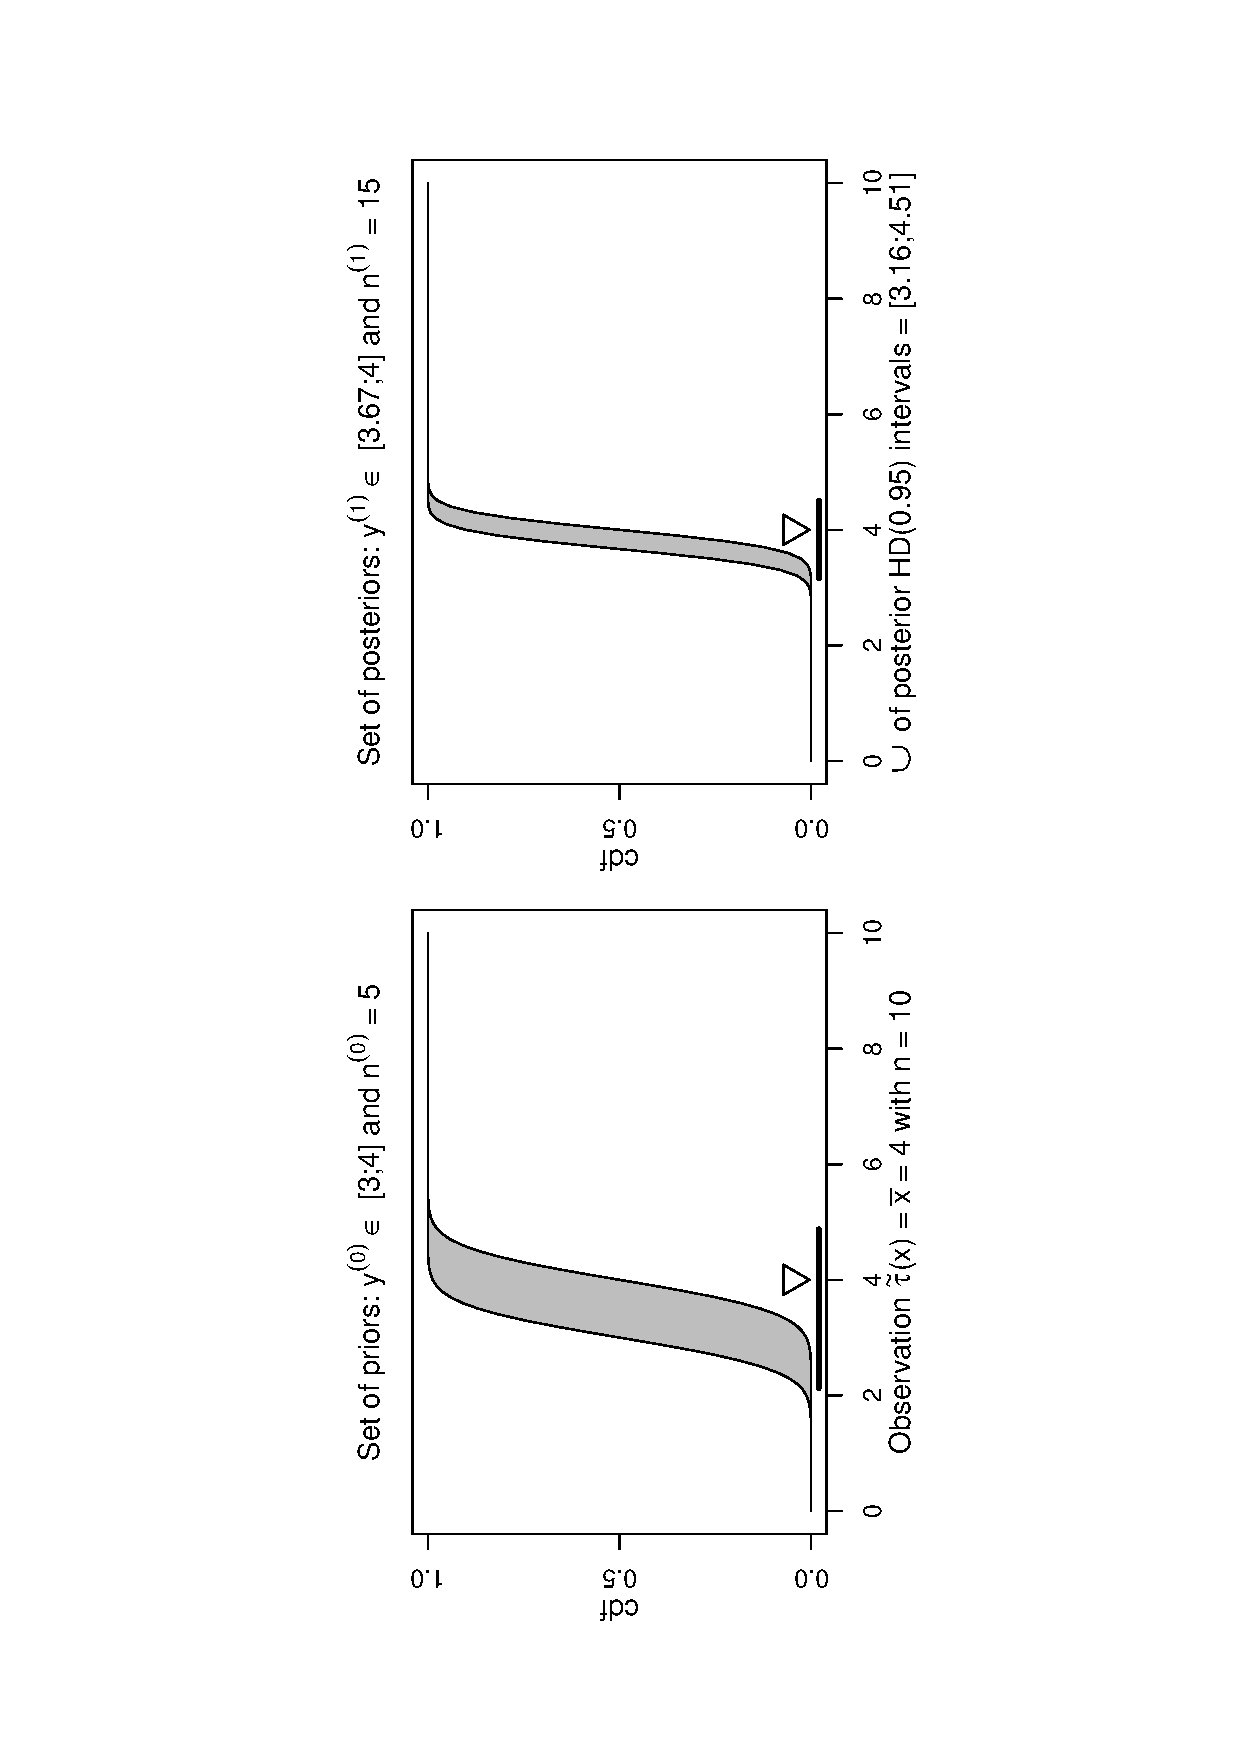
\includegraphics[trim = 20mm 50mm 20mm 50mm, clip, width=\textwidth]{fig/jstp-paper_nv_nfest_01-080331}%
\caption[\ymodel\ for samples from $\norm(\mu,1)$:
prior and posterior credal sets for data in accordance with prior beliefs.]%
{Prior (left) and posterior (right) credal sets for a sample
from $\norm(\mu,1)$ drawn as sets of normal cdfs. (Example~\ref{ex:ymodel-nv} in the
situation of no prior data conflict.)}
\label{fig:nv-nfest-nopdc}
\end{figure}


\begin{example}[Normal-Normal Model]
\label{ex:ymodel-nv}
%\noindent\textbf{Example 1a (continued).}
In the Normal-Normal model as presented in Section~\ref{sec:norm-norm},
$\yz$ corresponds to the expected value for $\mu$; the choice of $\YZ$ in application should thus be easy.
To simplify notation, we will assume here and later on that $\sigma^2_0 = 1$.
%Assuming the prior knowledge suggests values for $\mu$ in the range $[3;4]$, we define
%${\cal Y}\uz = [\ul{y}\uz ; \ol{y}\uz] = [3;4]$. For fixing
Let us assume $\YZ = [\yzl ; \yzu] = [3;4]$, and for fixing
$\nz$, suppose further that we are not very certain about
this prior range for $\mu$, but still think it is quite a reasonable
assumption, and so we base it on $5$ pseudo observations by choosing $\nz=5$,
giving a value of the variance for the prior distribution on $\mu$ of $\frac{1}{5}$.
%
%\medskip
%
Updating this prior with the i.i.d.\ sample $\x \in \reals^n$ yields%\vspace*{-0.8ex}%
\begin{align*} %\label{080306-nv_bsp_held}
\ynl &= \frac{\nz\yzl + \sum_{i=1}^n x_i}{\nz + n}, &%\hspace*{-1.5ex}
\ynu &= \frac{\nz\yzu + \sum_{i=1}^n x_i}{\nz + n}, &%\hspace*{-1.5ex}
\nn &= \nz + n\,.%\vspace*{-3.1ex}%
\end{align*}

To make this concrete, consider a sample of size $n = 10$
with $\ttau(\x) = \bar{x} = 4$.
Then $\YN = [\frac{55}{15} ; \frac{60}{15}] \approx [3.67 ; 4]$,
${\rm MPI}\un=\frac{1}{3}$ and $\nn = 15$. The posterior credal set
consists therefore of all convex combinations of normal
distributions with means in $[3.67 ; 4]$ and variance
$\frac{1}{15}$.
%
% ------------ verschoben anfang
%
Prior and posterior beliefs can be illustrated by the union of
credal intervals calculated as highest density (HD) intervals%
\footnote{See the concept of highest posterior density (HPD) intervals
as mentioned in Section~\ref{sec:beta-binom}, which used here also to
illustrate the prior state of knowledge.}
%HD intervals\footnote{For a given distribution, a HD interval
%(for \emph{h}ighest \emph{d}ensity) gives a set
%of most plausible values identified as the set %with the shortest range
%of values with highest density
%resulting / aggregating a certain amount of probability weight $\gamma$.}
for all distributions in the corresponding credal set.
As the normal distributions with mean $\yz \in \YZ$ are the extreme points of the prior credal set,
and the normal distributions are stochastically ordered with respect to the mean,
the prior union is the interval from the lowest lower border of HD intervals
(calculated from $\norm(\yzl, \frac{1}{\nz})$) to the highest upper border
(calculated from $\norm(\yzu, \frac{1}{\nz})$).
For a probability weight $\gamma = 0.95$, we get $[2.123;\, 4.877]$.
%
% ------------ verschoben ende
%
The posterior union of HD intervals is
$[3.161;\, 4.506]$ and, covering a much smaller range as a priori, shows
the decreasing of uncertainty obtained by the update step, also
reflected in a main parameter precision gain of ${\rm PG}=\frac{2}{3}$.
This update step is illustrated in Figure~\ref{fig:nv-nfest-nopdc},
where the prior and posterior credal set are displayed by the normal
cumulative distribution functions, the black lines indicating the
functions defined by the vertices of $\YZ$ and $\YN$, respectively. %\sidenote{statt: that constitute their vertices.}
The observation $\ttau(\x)$ is marked by the point of the triangle
in both graphs, and the prior and posterior union of HD intervals are marked
by a thick line in the graph for the prior and posterior set, respectively.
\end{example}

\begin{example}[Dirichlet-Multinomial Model]
\label{ex:ymodel-idm}
An \ymodel\ based on the Dirichlet-Multinomial Model as discussed in Section~\ref{sec:diri-multi}
is, for $\YZ = \Y$, equivalent to the imprecise Dirichlet model
(IDM, see Section~\ref{sec:idm-and-near-ignorance}), and was considered in Section~\ref{sec:fixedlearningparameter}
for the common-cause failure application.

In the usual applications of the IDM, the aim is to start with prior
ignorance; this is modelled by choosing $\YZ$ as the unit
simplex. For $\nz$ values of 1 or 2 are suggested. Here,
we must rely on the interpretation of $\nz$ as prior strength, as
there is no interpretation in terms of other
parameters as in Example~1a.
%
%\medskip
%
Considering prior knowledge for a three-category multinomial model
suggesting that extreme values for $\theta_1$ and $\theta_2$ are
implausible, one could choose
$\YZ = \{ \yz_1 \in [0.2;0.8] \times \yz_2 \in [0.2;0.8] \times \yz_3 \in [0;0.6]\}$,
where the upper bound for $\yz_3$ is a result of the unit
simplex constraint $\sum_{j=1}^k \yz_j = 1$.
In addition, we choose again $\nz=5$ as in Example~\ref{ex:ymodel-nv}.
%
%\medskip
%
Considering a sample of size $5$, where $3$ observations are of
category 1, and $2$ of category 2, we get $\nn = 10$ and the ranges
$\yn_1 \in [0.4 ; 0.7]$,
$\yn_2 \in [0.3 ; 0.6]$, and
$\yn_3 \in [0   ; 0.3]$
for the posterior class probabilities.
%For instance, the posterior
%probability for observing category two or three in the next draw
%is, by applying conjugacy, between $0.3$ and $0.6$.
In analogy to Example~\ref{ex:ymodel-nv}, this update step is illustrated with the
left and center graph of Figure~\ref{fig:idm-nfest-nopdc}, where
prior and posterior credal sets are represented by cutouts from a
plane in the three-dimensional parameter space. Each point in the
plane cutout for the prior set on the left graph represents a
certain combination of $\yz_1$, $\yz_2$, and $\yz_3$ by the
magnitude of coordinates. The same applies for the posterior set
depicted in the center graph. Some additional lines were drawn to
make locating the cutouts in space more easy.
\end{example}

\begin{figure}
\begin{tabular}{ccc}%
\hspace*{-1.2ex}% trim = l b r t
%\includegraphics[height=0.33\textwidth,angle=-90,bb = 100 65 520 385]{fig/jstp-paper_idm_nfest_01-080331.ps}%
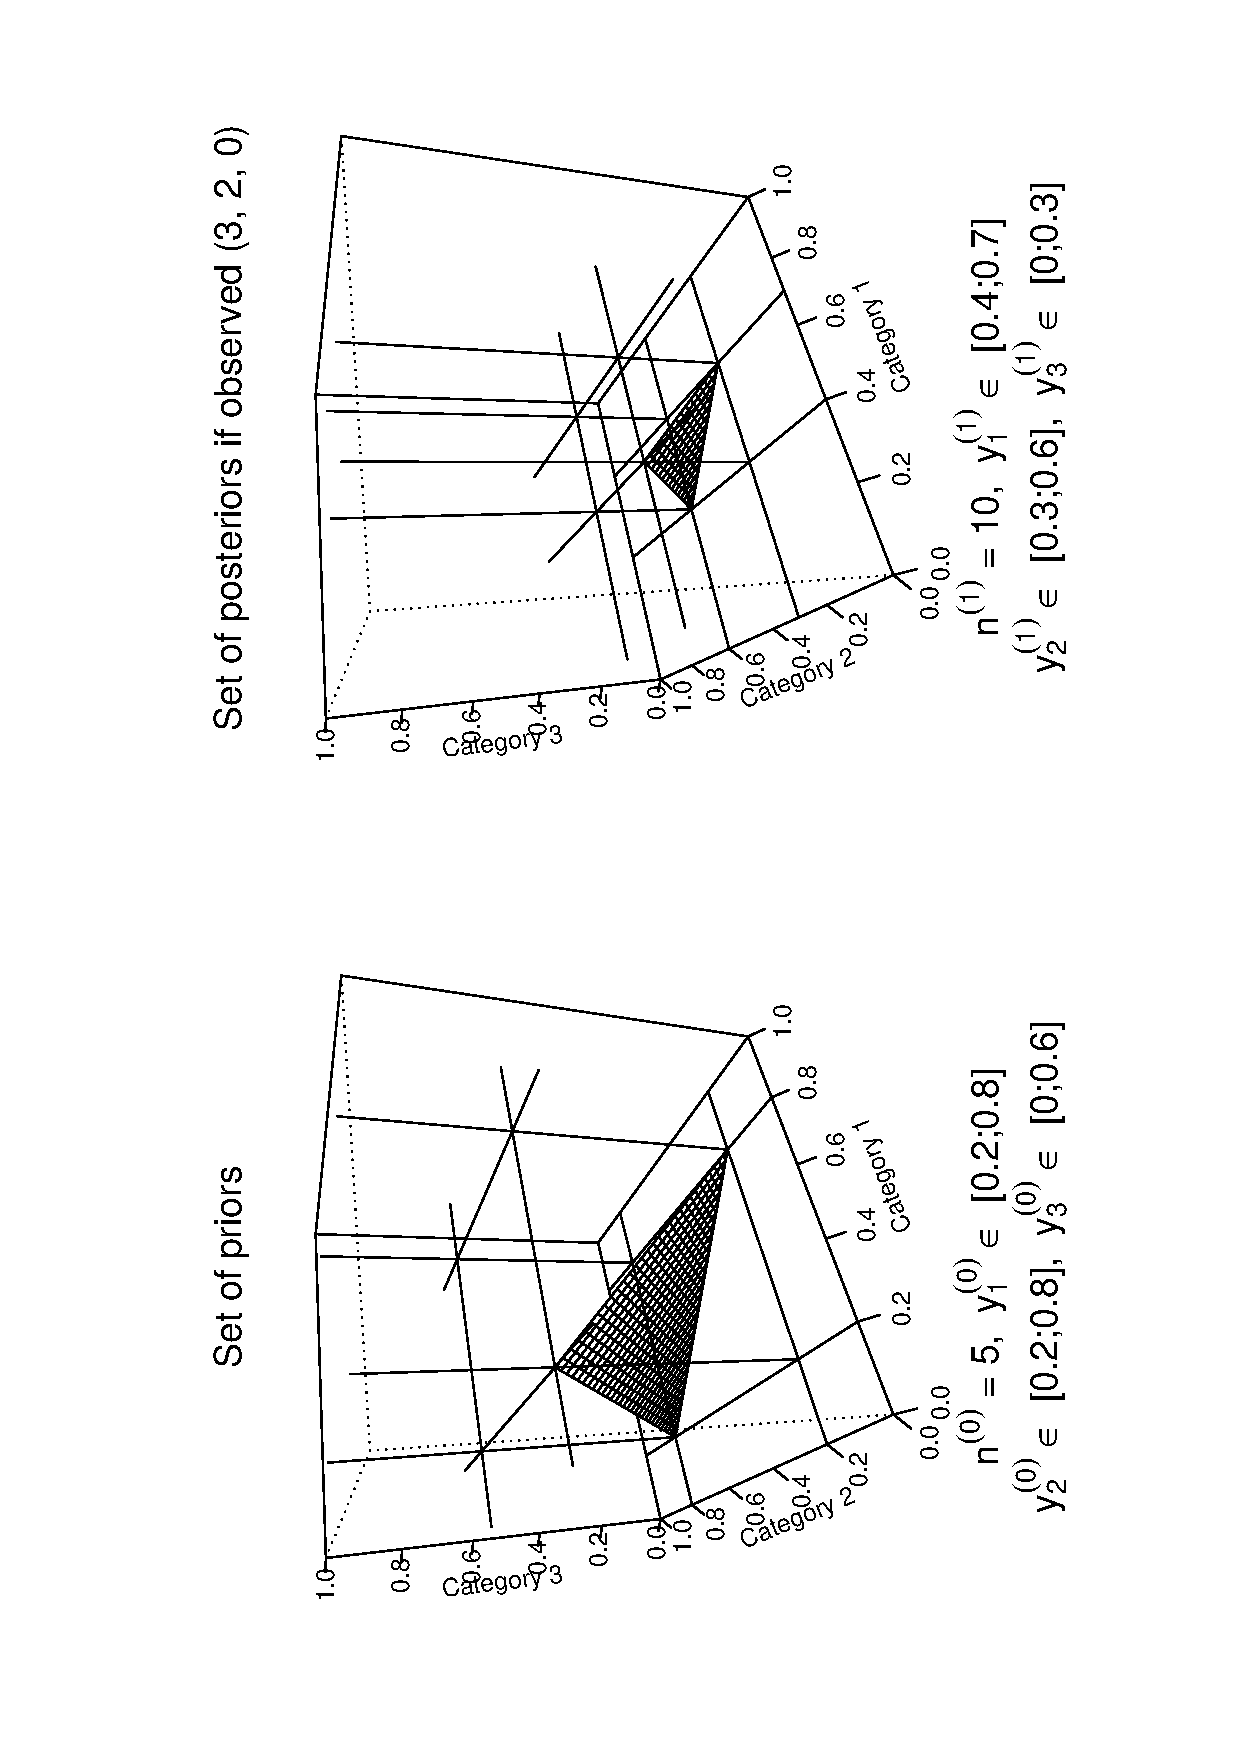
\includegraphics[trim =  20mm 25mm 150mm 20mm, clip, width=0.33\textwidth]{fig/jstp-paper_idm_nfest_01-080331}%
\hspace*{-1.2ex}%
&%
\hspace*{-1.2ex}%
%\includegraphics[height=0.33\textwidth,angle=-90,bb = 100 470 520 790]{fig/jstp-paper_idm_nfest_01-080331.ps}%
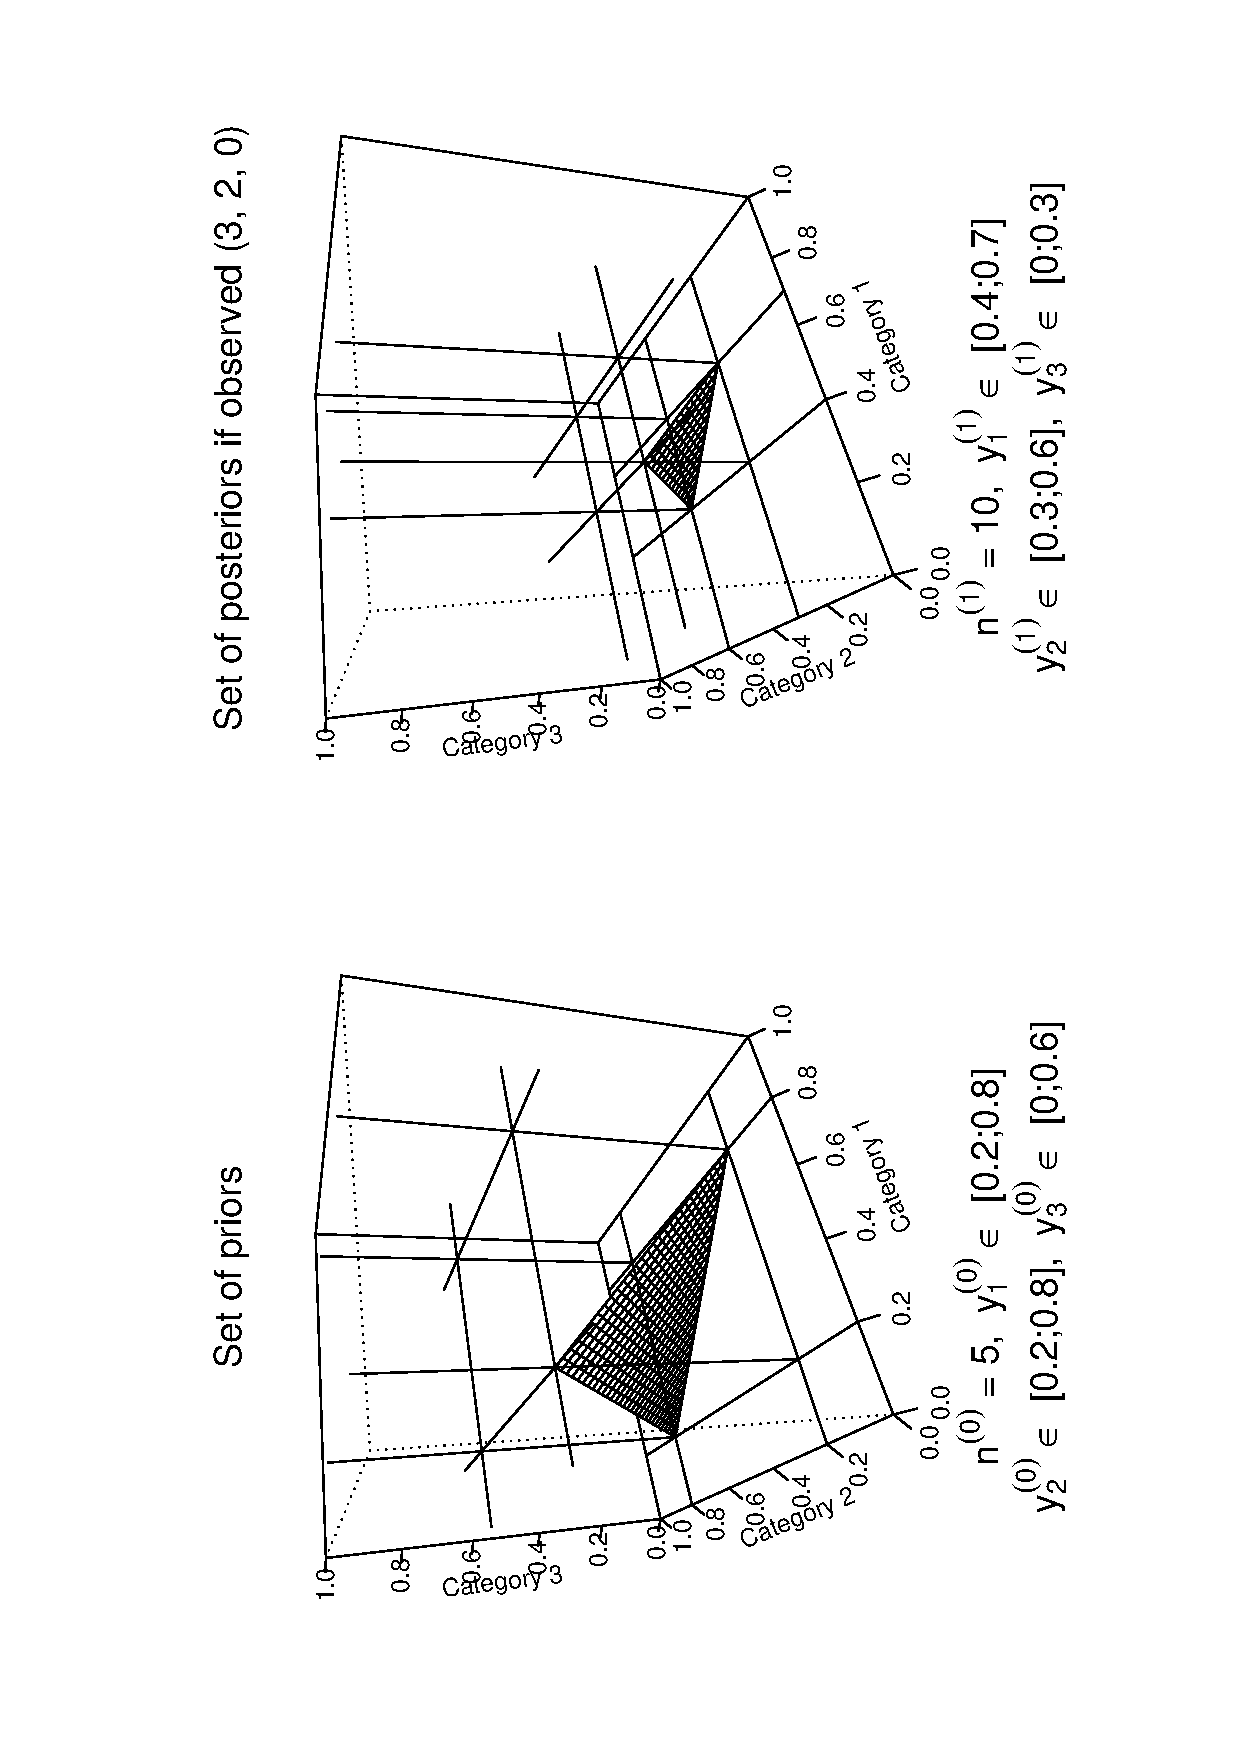
\includegraphics[trim = 150mm 25mm  20mm 20mm, clip, width=0.33\textwidth]{fig/jstp-paper_idm_nfest_01-080331}%
\hspace*{-1.2ex}%
&%
\hspace*{-1.2ex}%
%\includegraphics[height=0.33\textwidth,angle=-90,bb = 100 470 520 790]{fig/jstp-paper_idm_nfest_02-080331.ps}%
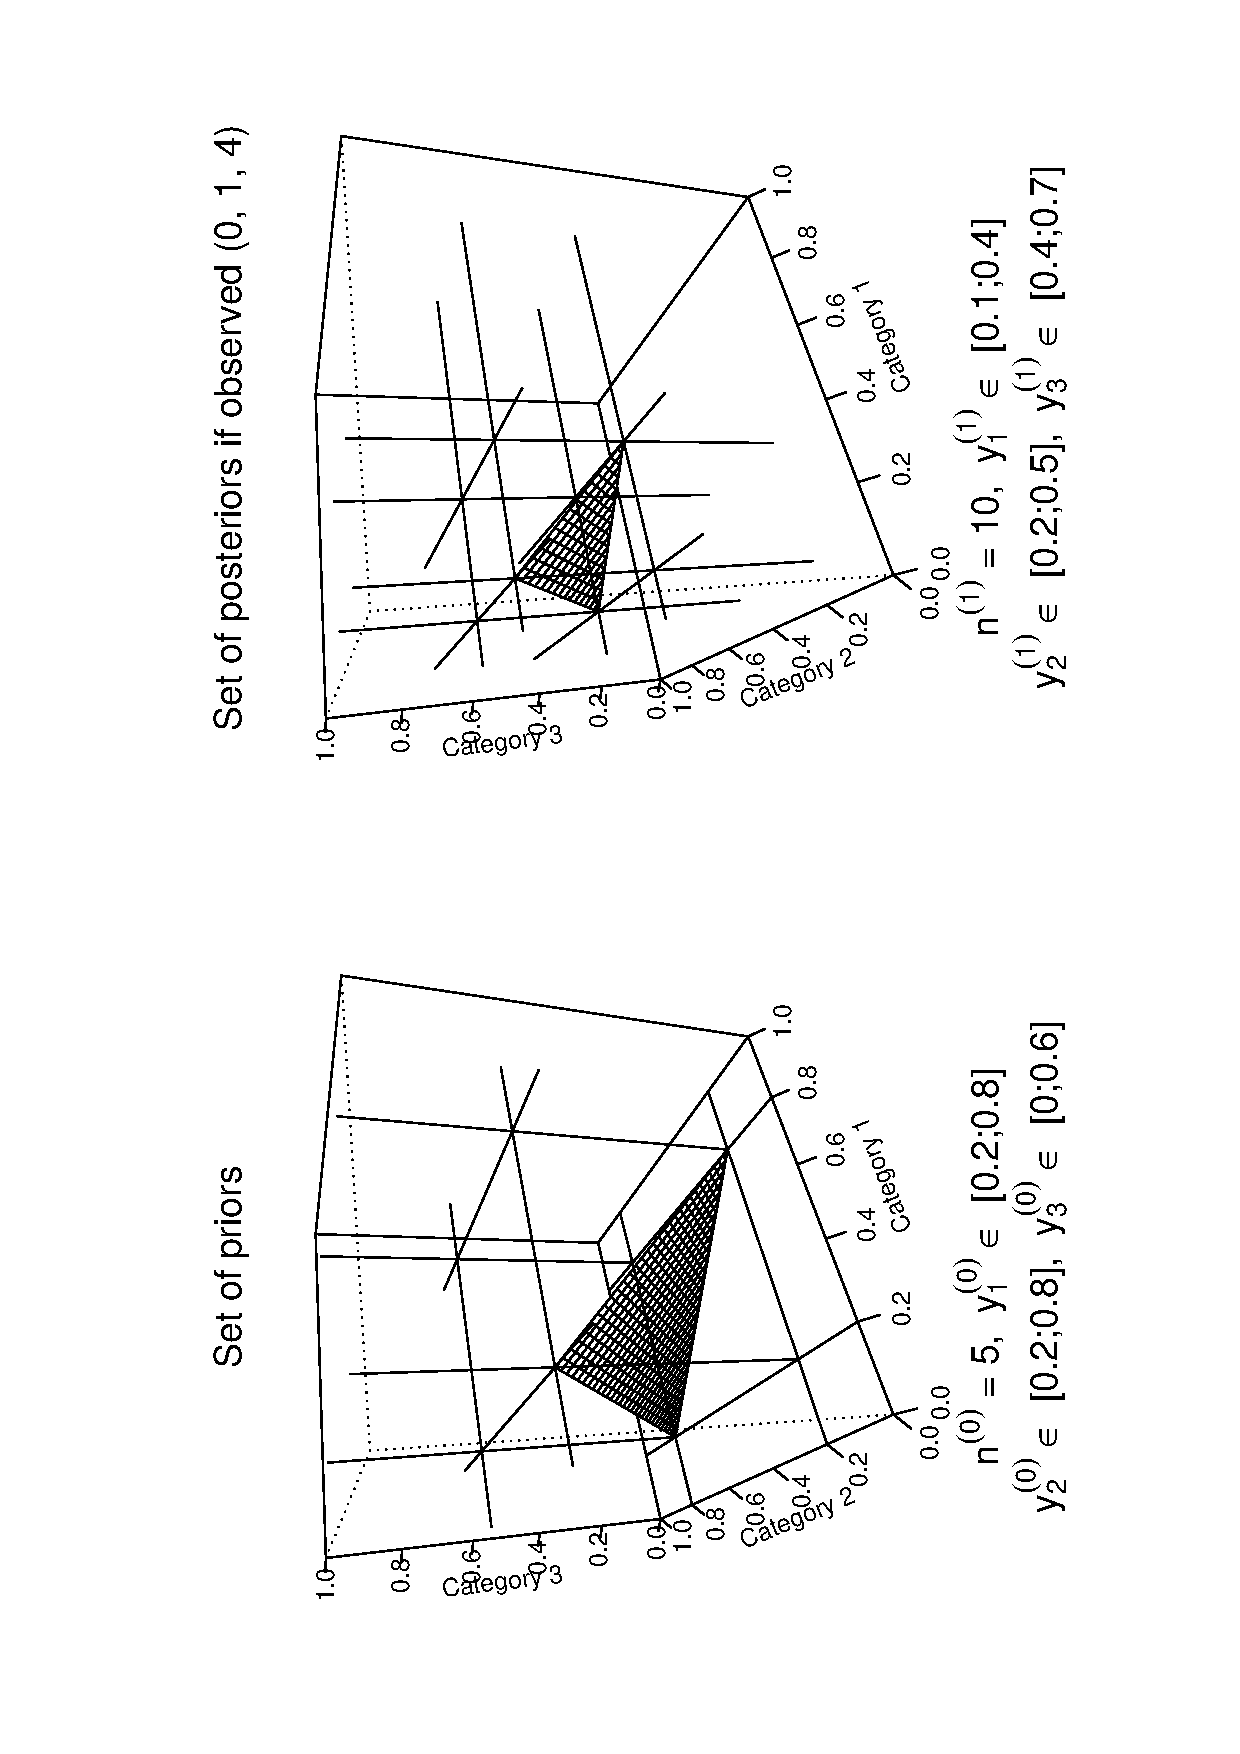
\includegraphics[trim = 150mm 25mm  20mm 20mm, clip, width=0.33\textwidth]{fig/jstp-paper_idm_nfest_02-080331}%
\hspace*{-1.2ex}%
\end{tabular}%
\caption[\ymodel\ for samples from $\mult(\btheta)$: prior and posterior credal sets
for data in accordance with and contrary to prior beliefs.]%
{Prior (left) and posterior (center, right) credal sets for samples from
$\mult(\btheta)$ in accordance with (center) and, as studied in
Section~\ref{section:fixednschlecht}, contrary to (right) prior
beliefs. Note that both posterior sets have the same shape and size and differ
only in location, in contrast to the ones depicted in Figure~\ref{fig:idm-nvar-nopdc}.}
\label{fig:idm-nfest-nopdc}
\end{figure}


\begin{remark} \label{remark:i-v}
%The following list contains important properties of
%inference in \emph{\ymodel s}, \thc{where the first three items} in
%essence \thcc{generalize results} that have been discussed in
%the literature for the IDM, where, as already said above, $n\uz$
%usually is denoted by $s$.\vspace*{-1.5ex}
Inference in \emph{\ymodel s} has the following important properties,
where the first three items in essence generalize results that have
been discussed in the literature for the IDM, where, as already said
above, $\nz$ usually is denoted by $s$.%
\footnote{See the discussion in Section~\ref{sec:gbicp-properties-criteria}.***}
\begin{enumerate}[i)]
\item The larger $\nz$ relative to $n$, the more weight is placed on
the prior knowledge expressed by $\YZ$, resulting in wider
posterior expectation intervals and larger ${\rm MPI}\un$.
\item For growing sample sizes $n$, the set $\YN$ will
converge towards a one-element set, as the weight of the `imprecise'
$\YZ$ decreases with respect to the `precise' sample
$\ttau(\x)$, ultimately resulting in an (almost)
precise posterior with ${\rm MPI}\un=0$ just as in
classical methods.
\item In particular, for $\nz = n$, the width of the posterior
expectation interval is half the width of the prior interval,
i.e., ${\rm MPI}\un = \frac{1}{2}{\rm MPI}\uz$.
This property is easily derived from \eqref{equ:ymodel-ydiff}
below, and provides another vivid interpretation of $\nz$.
\item Ceteris paribus, a smaller choice of $\YZ$ will result
in a smaller $\YN$, leading to more precise inference
statements as opposed to the choice of a larger $\YZ$.%
\footnote{This item has not been widely considered in
the context of the IDM, which typically is used to
describe inference from a state of prior ignorance.}
\item For the main posterior parameter imprecision, we obtain:
\begin{align}\label{equ:ymodel-ydiff}
{\rm MPI}\un &= \frac{\nz \left( \yzu - \yzl \right)}{\nz + n}.
\end{align}
\end{enumerate}
\end{remark}%\vspace*{-1.5ex}
While items i) -- iv) demonstrate the intuitively appealing
behavior of \ymodel s, we are seriously concerned with %respect to
the fact that ${\rm MPI}\un$ is independent of $\ttau(\x)$,
and, as studied in more detail in the next subsection, therefore
insensitive to prior-data conflict.


\subsubsection{\ymodel s and Prior-Data Conflict}
\label{section:fixednschlecht}
In the linear setting of \ymodel s, the generic concept of prior-data conflict
can be formalized by considering the distance of the observed quantity $\ttau(\x)$ to
its nearest prior guess $\yz \in \YZ$:
%
\begin{definition}[(Degree of) Prior-Data Conflict]\label{080307-defin-pdc}
For \ymodel s, the degree of prior-data conflict can be defined %naturally
as
\begin{equation}\label{se-071217}
%\Delta \left(\frac{\tau^n(x)}{n};\, \ul{y}\uz,\,\ol{y}\uz\right)
%= \inf \left\{ \left| \frac{\tau^n(x)}{n} - y\uz \right|: \ul{y}\uz \leq y\uz \leq \ol{y}\uz \right\}\,.
\Delta \left(\ttau(\x);\, \yzl,\,\yzu\right)
:= \inf \left\{ \left| \ttau(\x) - \yz \right|: \yzl \le \yz \le \yzu \right\}\,.
\end{equation}
Consequently, if
$\Delta \left(\ttau(\x);\, \yzl,\,\yzu\right) > 0$,
we have an instance of prior-data conflict.%
\footnote{Instead of $\Delta(\;\;) > 0$, one could also consider some
threshold $\Delta(\;\;) > \varepsilon > 0$ as a criterion for prior-data conflict, making
Definition~\ref{080307-defin-pdc} also reasonable for \model s.
However, with respect to Remark~\ref{remark8} below, we prefer $\varepsilon = 0$.}
\end{definition}
This Definition can be illustrated by, e.g., Example~\ref{ex:ymodel-nv}, where $\ttau(\x) = \bar{x}$
is the sample mean. A sample mean outside $\YZ$, the a priori assumed interval
of means for the normal distribution on $\mu$, is an instance of prior-data conflict.
If a sample mean of $8$ was observed in the numerical example discussed above, where
$[\yzl ; \yzu] =[3;4]$ had been assumed, we would obtain $\Delta(\;) = 4$,
formalizing our intuition that prior-data conflict is at hand.

As we argued in Sections~\ref{sec:motivation:pdc} and \ref{sec:jstp-intro},
imprecise probability models that allow to take prior information into account
should lead to more imprecision if prior-data
conflict is present than in situations where it is not.
%
It is easy to see that \ymodel s do not fulfill this property
because the main parameter posterior imprecision in
\eqref{equ:ymodel-ydiff} does not depend on the sample statistic
$\ttau(\x)$. Thus, for any sample of size $n$, an \ymodel\ leads
to the same main parameter posterior precision gain
whether the sample supports the prior assumptions modelled in
$\YZ$ or it confronts them. As a consequence of the
Bayesian paradigm that all inference is only allowed to depend on
the posterior, this holds also for all derived quantities
like HD intervals. To make this concrete,
let us continue Examples~\ref{ex:ymodel-nv} and \ref{ex:ymodel-idm}.

\begin{figure}
%\includegraphics[height=\textwidth,angle=-90,bb = 165 60 440 765]{fig/jstp-paper_nv_nfest_02-080331.ps}%
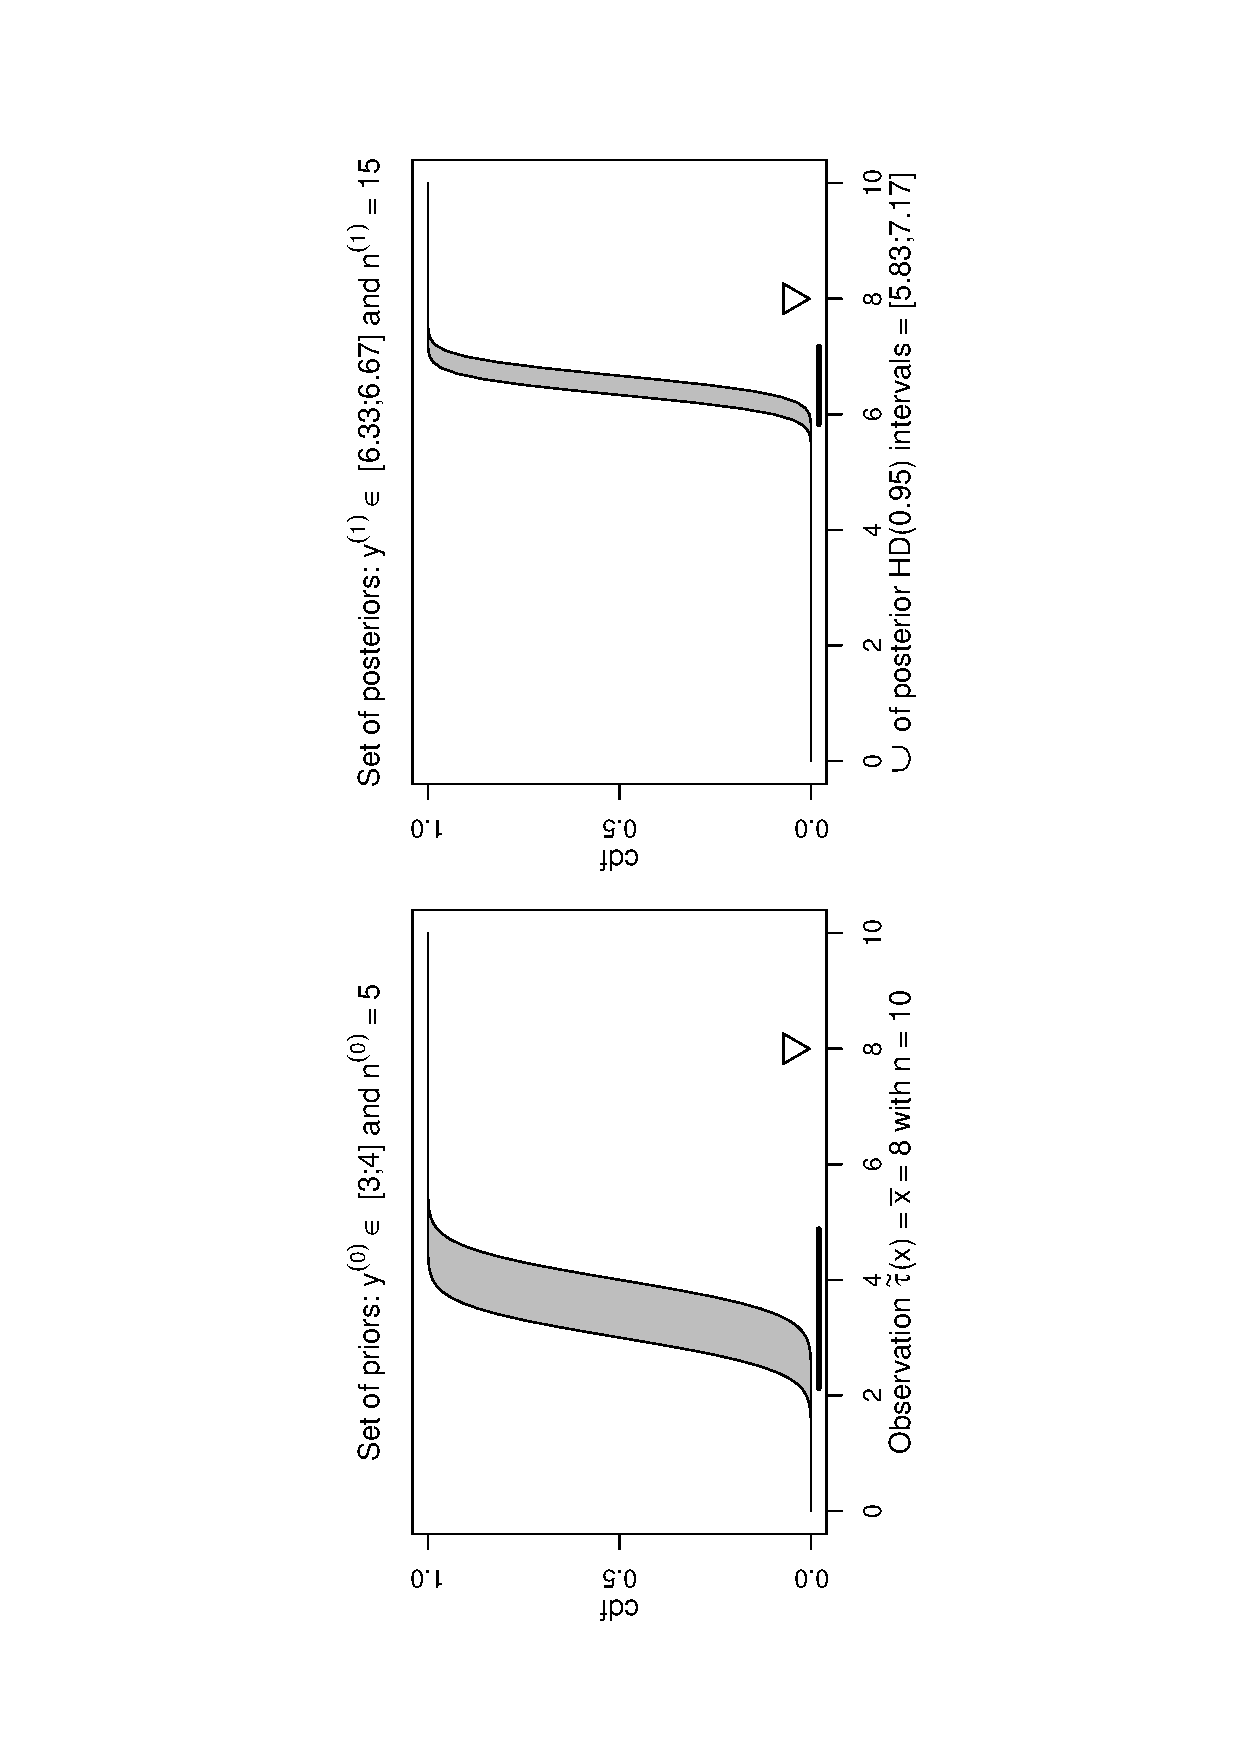
\includegraphics[trim = 20mm 50mm 20mm 50mm, clip, width=\textwidth]{fig/jstp-paper_nv_nfest_02-080331}%
\caption[\ymodel\ for samples from $\norm(\mu,1)$: prior and posterior credal sets for data contrary to prior beliefs.]%
{In \ymodel s, an observation contrary to prior beliefs leads to
the same amount of imprecision as an observation in accordance with prior
beliefs (see Figure~\ref{fig:nv-nfest-nopdc}).  Generalized \ymodel s overcome this
deficiency, as visualized in Figure~\ref{fig:nv-nvar-vertfu}.}
\label{fig:nv-nfest-pdc}
\end{figure}

\begin{example}[Normal-Normal Model, continued]
\label{ex:jstp-5}
%\noindent\textbf{Example 1a (continued).}
Assume, in the situation considered in Section~\ref{070514-secImpPriorLUCK-QdC},
that the sample had led to $\ttau(\x) = 8$,
suggesting the mean $\mu$ to be nearer to $8$ than to the range $[3;4]$ assumed
for it before having seen the sample.
Then $\YN = [\frac{95}{15} ; \frac{100}{15}] \approx [6.33 ; 6.67]$ and again
$\nn = 15$. The posterior range of expected values for $\mu$ has now moved
towards the value suggested by the sample, but we have the same
posterior main parameter imprecision $\frac{1}{3}$ as in the
case with $\ttau(\x) = 4$, which was not conflicting with the prior
assumptions. Intuitively, this fact gets maybe more perplexing when
considering the union of posterior HD intervals: For $\ttau(\x) = 4$,
it is $[3.161;\, 4.506]$, covering a length of $1.345$; for
$\ttau(\x) = 8$, it is $[5.827;\,7.172]$, covering the very same
length, and therefore -- although being completely surprised by the
outcome of the sample -- we would not be more cautious.
These disturbing results are illustrated in Figure~\ref{fig:nv-nfest-pdc}.
\end{example}

\begin{example}[Dirichlet-Multinomial Model, continued]
\label{ex:jstp-6}
%\noindent\textbf{Example 1b (continued).}
Here, the same phenomenon occurs:
Having observed categories 1 to 3 now $0$, $1$, and $4$
times, respectively, $\YN$ covers the same area, despite of the clear conflict of these
observations with the prior knowledge expressed in $\YZ$,
and has only moved in location, as can be seen
in the right graph of Figure~\ref{fig:idm-nfest-nopdc}.
\end{example}


\subsection{Improved Imprecise Priors for Inference in \model s}
\label{sec:4-gw-071216}

There do exist some imprecise probability models that react on
prior-data conflict in reasonable ways. The approaches by
\textcite{1991:pericchi} and \textcite{1994:coolen}
are restricted to specific one-parameter situations with a different type
of models for the prior. \textcite{2005:whitcomb}, on
the other hand, by partially relying on models from the exponential
family, considers closely related classes of underlying
distributions without using their specific structure. The important
hint for properly handling prior-data conflict in
\model s is again obtained from \textcite{1991:walley}.
In \S 5.4, he discusses prior-data conflict in the imprecise
Beta-Binomial model,%
\footnote{See Section~\ref{sec:beta-binom}.}
which is a special case of the Imprecise
Dirichlet Model recalled in Example~\ref{ex:ymodel-idm}. His successful idea is to
vary the hyperparameter $s$ in addition. Additionally, he also
briefly mentions the normal case underlying Example~\ref{ex:ymodel-nv}
\parencite[\S 1.1.5 (k)]{1991:walley}, where he suggests to use an
imprecise prior with an imprecise variance. In the light of the
general framework of \model s, both exemplary solutions
can be subsumed under the idea to use an imprecise prior strength,
thus weighting prior and sample information in
\eqref{equ:shifttrans} in a more flexible way, i.e.\ to vary
additionally the prior strength parameter $\nz$ in some set $\NZ$.
Indeed this way to proceed will turn out to be successful.
We start by describing the powerful generalisation we want to
propose in more detail and then discuss some of its basic
properties.
%
%
%
%
\begin{definition}[\nymodel s]\label{071221-def}%
%Consider the Imprecise Probability model as described in \mycite{QdC} %Quaeghebeur and de Cooman (2005),
%or, more generally, a \textsc{LUCK}-model,
Consider the situation of Definitions~\ref{070503-defin1}
and \ref{071219-def2}, and a set of LUCK-models
$\big(p(\vartheta),p(\vartheta\mid\x)\big)$ that is produced by
$\yz$ varying in some set $\YZ \subset \Y$
and, in addition, $\nz$ varying in a set $\NZ \subset \posreals$.
Let furthermore again the credal sets ${\cal M}$ and ${\cal M}_{|\x}$ consist
of all convex mixtures obtained from this variation of $p(\vartheta)$ and
$p(\vartheta\mid\x)$. Then $\big({\cal M}, {\cal M}_{|\x}\big)$ is
called the corresponding \emph{\nymodel } based on $\YZ$ and $\NZ$.
\end{definition}

\begin{remark}
Again, by construction, when ${\cal M}$ is used as an
imprecise prior,  ${\cal M}_{|\x}$ is the corresponding posterior. It is obtained
as the set of all convex mixtures of
distributions defined by the parameter set
\begin{equation*}
%\left\{\!\! \left. \left(\!n\uo,\, y\uo\! \right) \; \right| \; n\uo = n\uz + n,\, y\uo = \frac{n\uz y\uz + \tau(x)}{n\uz+n},\,
%n\uz \in {\cal N}\uz,\, y\uz \in {\cal Y}\uz \!\right\}
\left\{ \left. \left(\nn,\yn\right) \; \right| \, \nn = \nz + n,\, \yn = \frac{\nz\yz + \tau(\x)}{\nz + n},\,
\nz \in \NZ,\, \yz \in \YZ \right\}\,.
\end{equation*}
Note that the set of posterior parameters is not a cartesian product, i.e., rectangular. However,
extreme values for the main posterior parameter $\yn$ are still easy to derive:%
\footnote{As $\frac{d}{d \yz}\, \yn = \frac{\nz}{\nz + n} \ge 0 \;
\forall\, n,\, \nz,\,\tau(\x)$, it holds that $\yn$ is growing in
$\yz$ regardless of the value of $\nz$, and thus, for obtaining
$\ynu$, we must insert $\yzu$, and for obtaining
$\ynl$, we must insert $\yzl$ in \eqref{070305-4}, just as
in \ymodel s, where $\nz$ is fixed. Then, with
$\frac{d}{d \nz}\, \yn  = \frac{\yz n - \tau(\x)}{(\nz + n)^2}$, we see that $\yn$
is growing in $\nz$ if $\yz > \ttau(\x)$ and decreasing in
$\nz$ if $\yz < \ttau(\x)$, leading to
Equations~\eqref{equ:uly1-071206} and \eqref{equ:oly1-071206}.}

\begin{align}
\ynl &= \label{equ:uly1-071206}
\begin{cases}
\frac{\nzu \yzl + \,\tau(\x)}{\nzu + n} & \text{if}\quad \ttau(\x) \ge \yzl\\[1.5ex]
\frac{\nzl \yzl + \,\tau(\x)}{\nzl + n} & \text{if}\quad \ttau(\x) <   \yzl
\quad\Longleftrightarrow\quad \text{prior-data conflict}
\end{cases} \\[1ex]
\ynu &= \label{equ:oly1-071206}
\begin{cases}
\frac{\nzu \yzu + \,\tau(\x)}{\nzu + n} & \text{if}\quad \ttau(\x) \le \yzu\\[1.5ex]
\frac{\nzl \yzu + \,\tau(\x)}{\nzl + n} & \text{if}\quad \ttau(\x) >   \yzu
\quad\Longleftrightarrow\quad \text{prior-data conflict}.
\end{cases}
\end{align}
\end{remark}

For minimising and maximising $\yn$, the value $\nzl$ is
used only in the situation of prior-data conflict, that is, if
$\ttau(\x) \notin \YZ$.
When no prior-data conflict occurs, the extreme values are attained for $\nzu$.
%
Therefore, the fixed value of $\nz$ in \ymodel s in the spirit of \textcite{2005:quaeghebeurcooman} can be
seen as the upper border of an implicit set $\NZ$, and
considering only a fixed $\nz$ means that prior-data conflict is neglected.

On the other hand, if observations are such that
$\ttau(\x) \in \left[\yzl;\,\yzu\right]$, then
no prior-data conflict is present, and inference in \nymodel s
leads to very similar results as inference in \ymodel s.%
\footnote{From \eqref{equ:uly1-071206} and \eqref{equ:oly1-071206}
it gets clear why varying $\nz$ in addition does change the
update step in the desired way. When $\ttau(\x) < \yzl$,
then $\nzu$ is still used to calculate $\ynu$, but
$\nzl$ to calculate $\ynl$. The use of $\nzl$ instead
of $\nzu$ results in a lower value for $\yzl$, as then
more weight is given to $\ttau(\x)$ with respect to
$\yzl$. (Equation~\eqref{equ:shifttrans} makes this most
visible.) The same type of reasoning applies for the case
$\ttau(\x) > \yzu$, where $\nzu$ is still used to
calculate $\ynl$, but $\nzl$ to calculate $\ynu$.}

\begin{remark}\label{remark8}
By construction, the attractive properties of inferences by
\ymodel s formulated in i) to iv) of Remark~\ref{remark:i-v}
are still satisfied in our extended model. Now
also in addition prior-data conflict is handled in a
convincing way: Considering the relationship between the main
parameter posterior imprecision defined as in
\emph{\eqref{071214-4}} and the degree of prior-data conflict
as defined in \emph{\eqref{se-071217}},%
\footnote{Remark~\ref{071221-remark} and Definition~\ref{080307-defin-pdc} can directly be applied also to \nymodel s.}
the very same results as derived by \textcite[p.~224]{1991:walley}
for the two-category Dirichlet-Multinomial model hold in general
for any \nymodel: %\vspace*{-1.0ex}

%Using the update rules for varying $n\uz$, we get,
%just as described in Walley (1991, p.~224) for a two-category IDM,
%a posterior range of
%\vspace*{-3.0ex}
\begin{align*}
{\rm MPI}\un &= \frac{\nzu (\yzu - \yzl)}{\nzu + n}
                + \Delta \left(\ttau(\x);\, \yzl,\,\yzu\right)
                  \, \frac{n (\nzu - \nzl)}{(\nzu + n)(\nzl + n)}\,.%
\end{align*}
%\vspace*{-1.0ex}
It is only through $\Delta(\;)$ that ${\rm MPI}\un$ is 
depending on the actual shape of observation $\x$ besides its size
$n$, and increasing it if prior-data conflict occurs. When no
prior-data conflict is present, $\Delta \left(\ttau(\x);\,\yzl,\,\yzu\right) = 0$,
and we have the same amount of posterior imprecision in substantial parameters as in \emph{\ymodel s},
given by \emph{\eqref{equ:ymodel-ydiff}}.

Consequently, Walley's \parencite*[\S 5.4, footnote~3]{1991:walley} observation
that the factor to $\Delta(\;)$ gets maximal if $n = \big(\nzl\nzu\big){}^\frac{1}{2}$
remains valid. Then, the main parameter posterior imprecision
is maximal for a given degree of conflict, implicitly telling that
then the weight of the prior and sample must be the same, as more
weight on any of them compared to the other (preferring one source
of information to the other) would lead to a less wide $\YN$.
This fact gives additional orientation for choosing $\NZ$,
by considering the global strength of prior knowledge,
being equivalent to $\ul{\ol{n}}\uz := \big(\nzl\nzu\big){}^\frac{1}{2}$.
\end{remark}

\begin{figure}
%\includegraphics[height=\textwidth,angle=-90,bb = 90 60 515 770]{fig/jstp-paper_nv_nvar_vertfu01_081128.ps}%
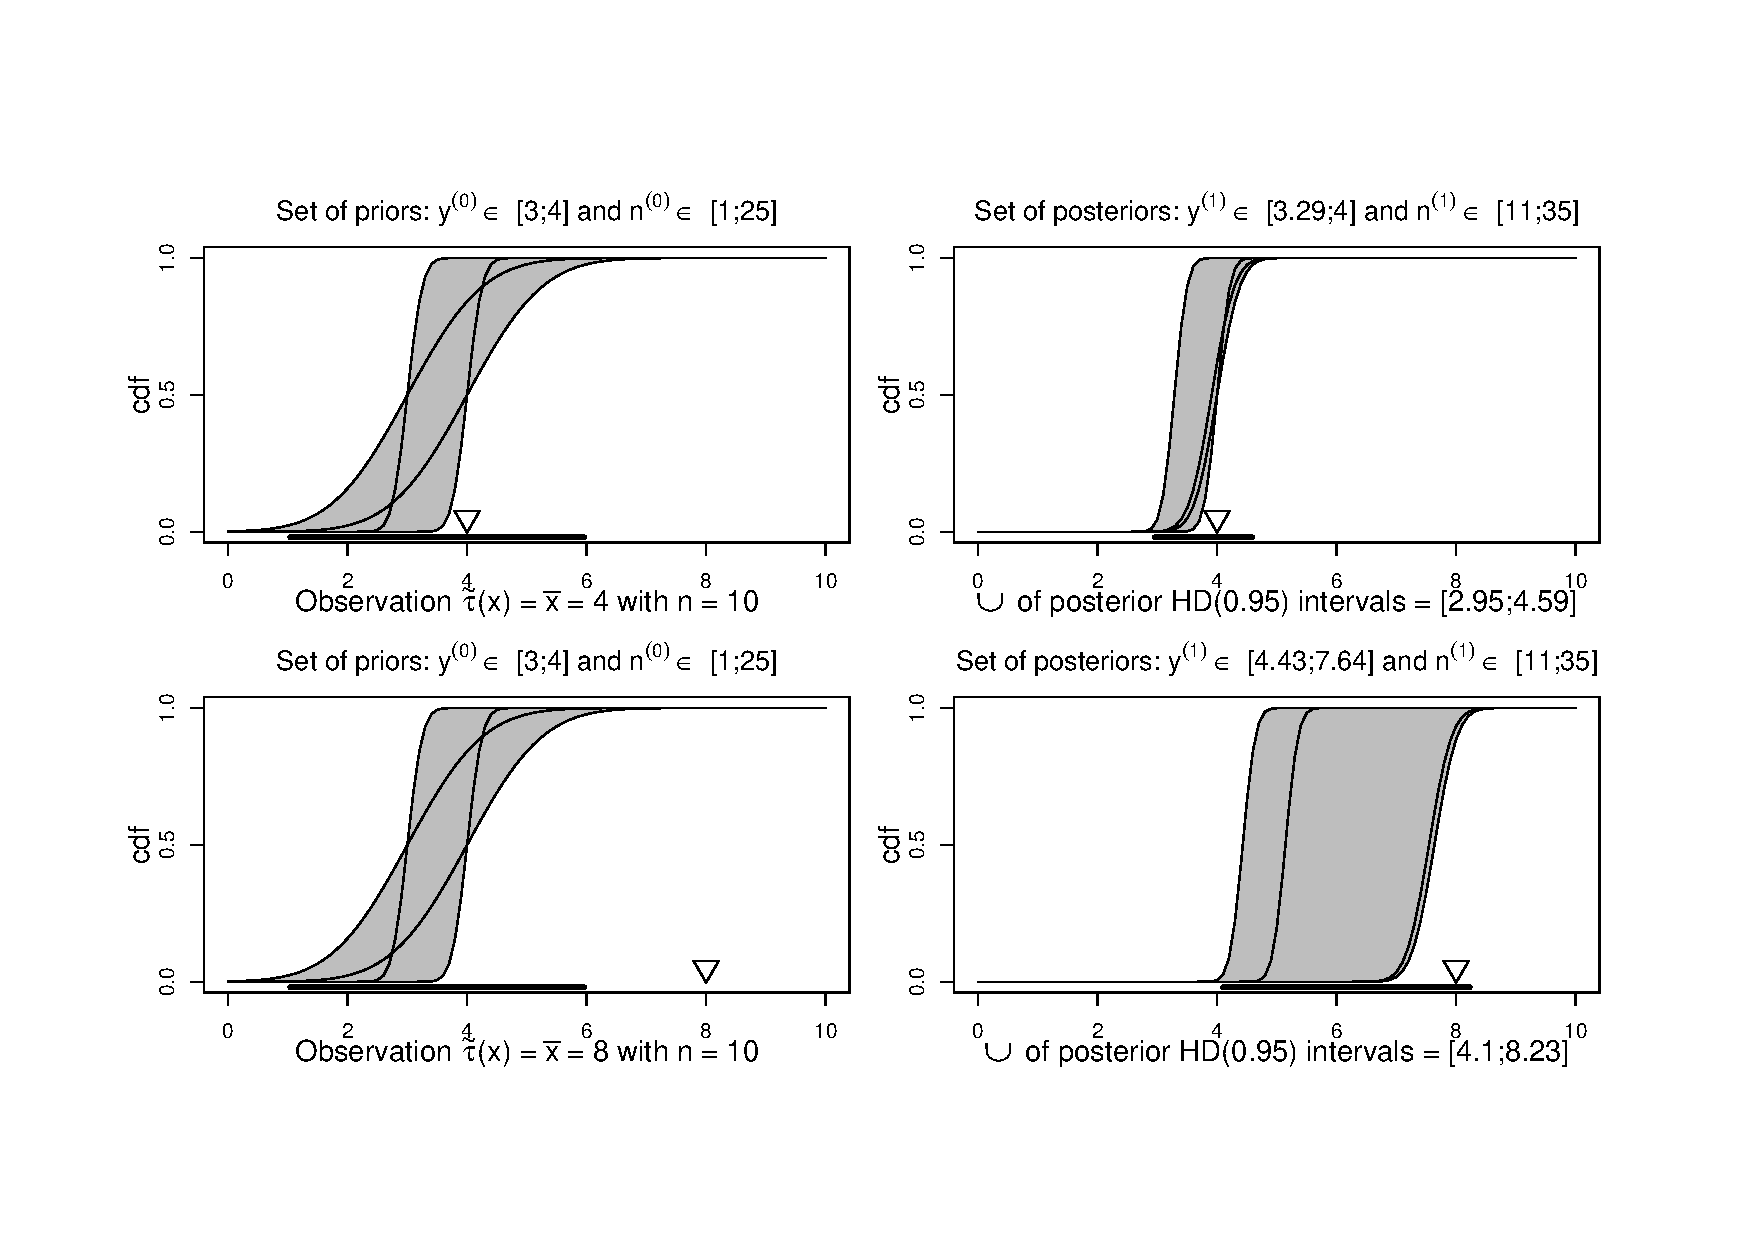
\includegraphics[trim = 20mm 20mm 20mm 25mm, clip, width=\textwidth]{fig/jstp-paper_nv_nvar_vertfu01_081128}%
\caption[Generalised \ymodel\ for samples from $\norm(\mu,1)$:
prior and posterior credal sets for data in accordance with and contrary to prior beliefs.]%
{Prior (left) and posterior (right) credal sets for samples from
$\norm(\mu,1)$ in accordance with (upper) and contrary to (lower)
prior beliefs. With \nymodel s, the posterior set in the latter case is
significantly larger than in the former, leading to more cautious inference as desired.}
\label{fig:nv-nvar-vertfu}
\end{figure}


\subsection{Illustration of the Generalised \ymodel}
\label{sec:illu} 

The theoretical considerations in Section~\ref{sec:4-gw-071216} are now
illustrated by means of Examples~\ref{ex:ymodel-nv} -- \ref{ex:jstp-6},
and some simulated data for larger sample sizes.

\begin{example}[Normal-Normal model, continued]
\label{ex:jstp-7}
For the case of the Normal-Normal Model (Examples~\ref{ex:ymodel-nv} and \ref{ex:jstp-5}),
the behavior of an appropriate \nymodel\ is shown for the situations previously
modeled with an \ymodel\ as depicted in
Figures~\ref{fig:nv-nfest-nopdc} and \ref{fig:nv-nfest-pdc}. In
Figure~\ref{fig:nv-nvar-vertfu}, the top row shows the updating in
absence of prior-data conflict, whereas the lower row displays
the update step in presence of prior-data conflict.
Again, the vertices of the credal set, the set of normal
distribution functions, is represented by the shaded area,
and the lines indicate the distributions that are obtained by updating the four
extreme distributions from $\NZ \times \YZ$.

Contrary to the \ymodel, also a range of variances is considered in the
prior, allowing for reasonable posterior inference, as can be seen
in the right hand graphs: when the prior model is consistent with
the observation $\ttau(\x) = \bar{x}$, a similar union of posterior HD
intervals is obtained as for the model displayed in
Figure~\ref{fig:nv-nfest-nopdc}; when instead prior assumptions and
data are conflicting, the posterior credal set reflects our
uncertainty on which to trust, being substantially larger than the
prior credal set. Therefore, the union of posterior HD intervals as
indicated by the thick line in the lower right graph is not only
wider than in the absence of prior-data conflict as seen in the top
right graph, but not much shorter than its prior counterpart, which is $[1.040;\, 5.960]$.
In order to give comparable results, $\NZ$ was chosen to give the same global prior strength as the
\ymodel\ for Example~\ref{ex:ymodel-nv} by fixing $\ul{\ol{n}}\uz=5$ and a minimal prior strength
$\nzl = 1$, resulting in $\nzu = 25$.
\end{example}

\begin{figure}
%\fbox{%
\begin{tabular}{ccc}%
\hspace*{-1.2ex}%
%\includegraphics[height=0.33\textwidth,angle=-90,bb = 100 65 520 385]{fig/jstp-paper_idm_nvar_zeile1-080331.ps}%
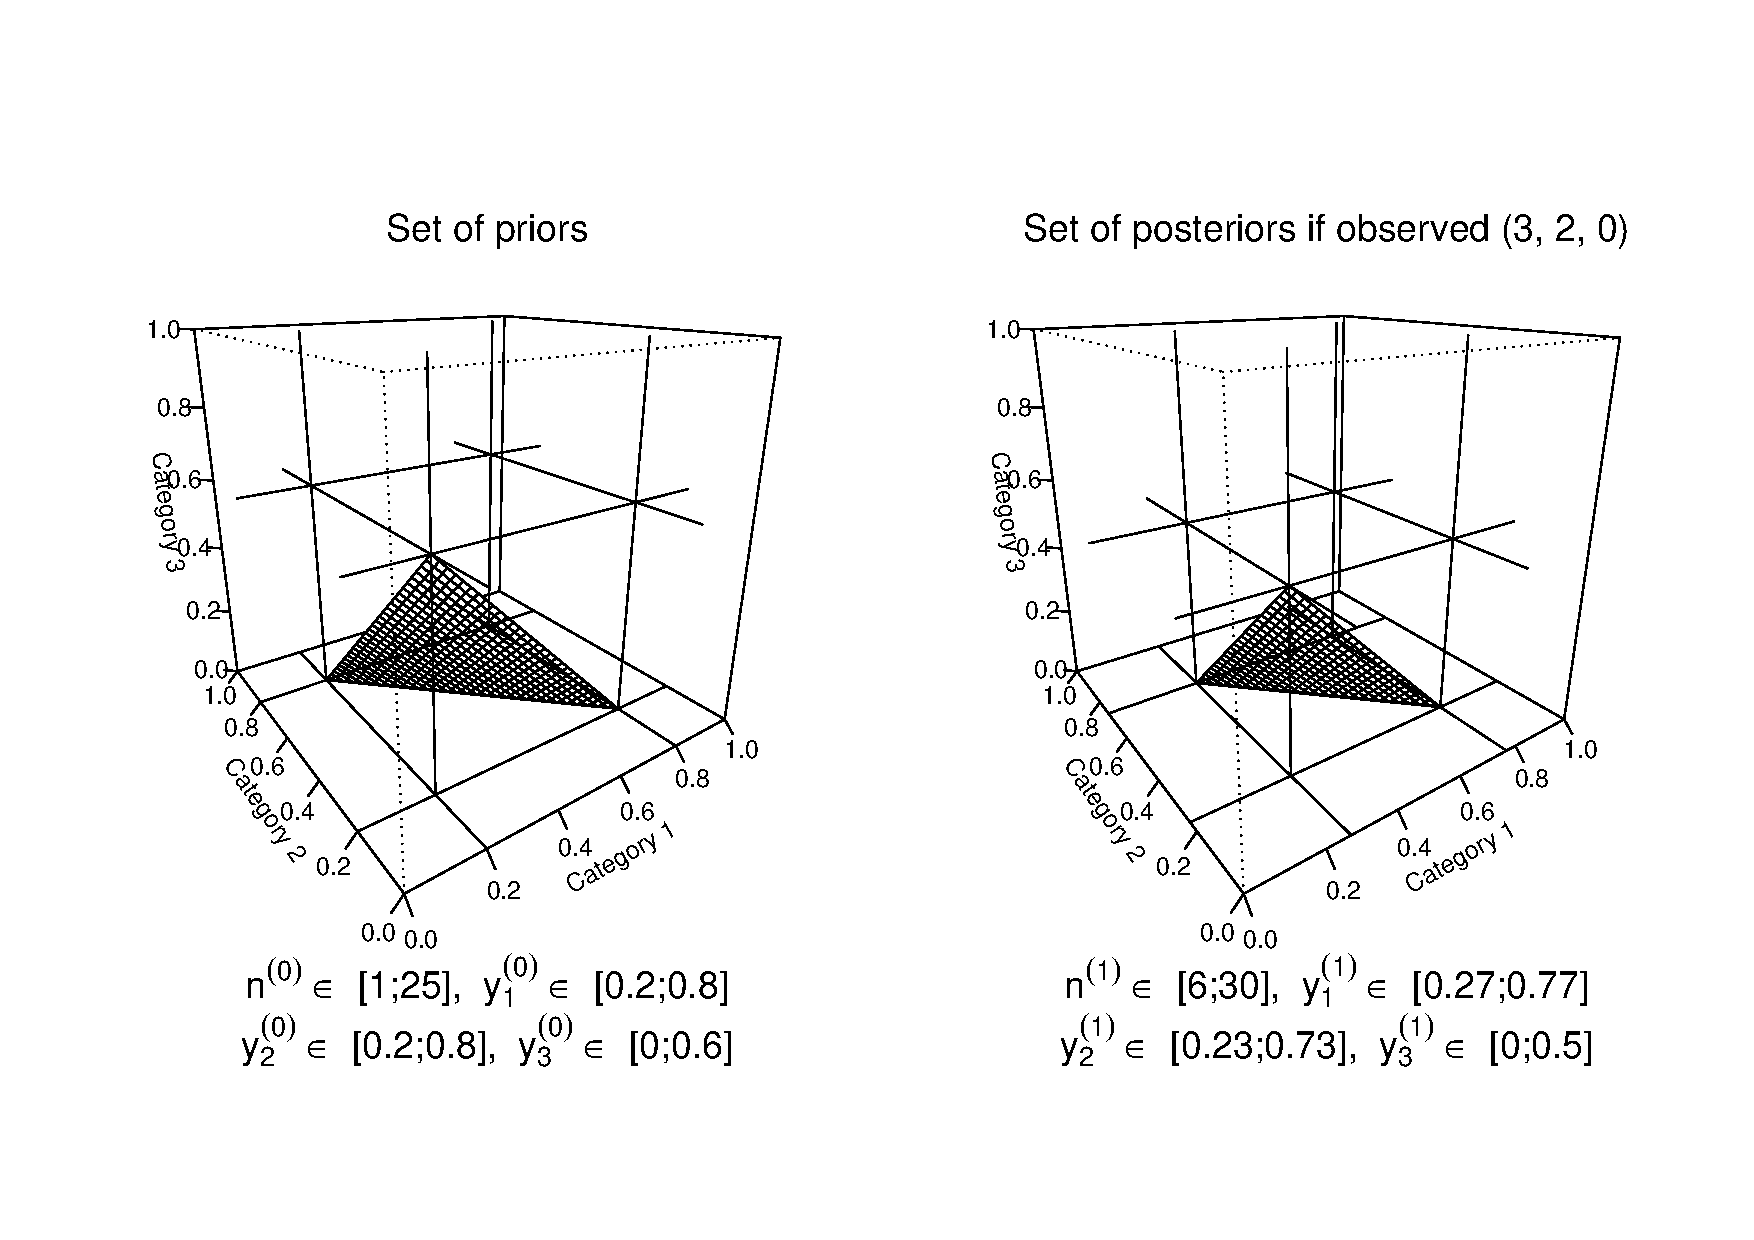
\includegraphics[trim =  20mm 25mm 150mm 20mm, clip, width=0.33\textwidth]{fig/jstp-paper_idm_nvar_zeile1-080331}%
\hspace*{-1.2ex}%
&%
\hspace*{-1.2ex}%
%\includegraphics[height=0.33\textwidth,angle=-90,bb = 100 470 520 790]{fig/jstp-paper_idm_nvar_zeile1-080331.ps}%
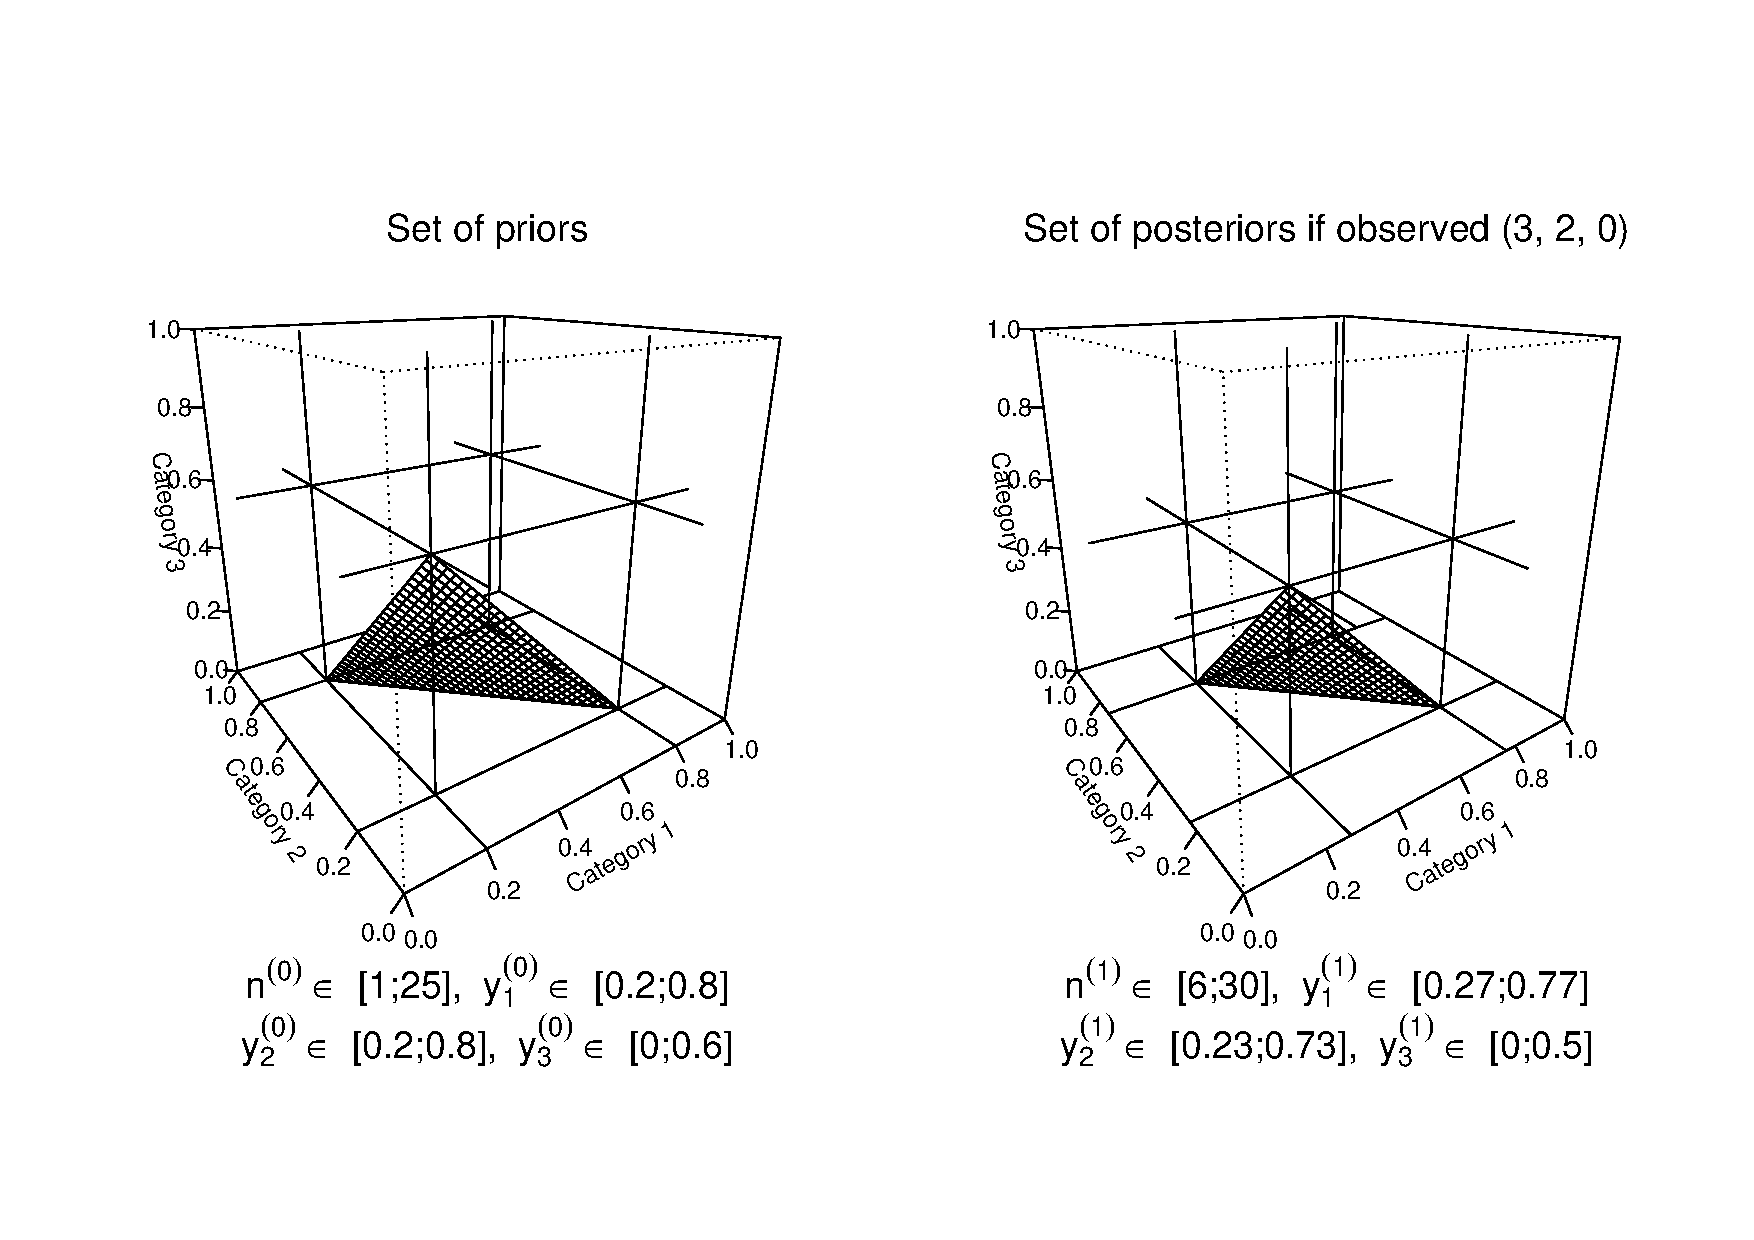
\includegraphics[trim = 150mm 25mm  20mm 20mm, clip, width=0.33\textwidth]{fig/jstp-paper_idm_nvar_zeile1-080331}%
\hspace*{-1.2ex}%
&%
\hspace*{-1.2ex}%
%\includegraphics[height=0.33\textwidth,angle=-90,bb = 100 470 520 790]{fig/jstp-paper_idm_nvar_zeile2-081205.ps}%
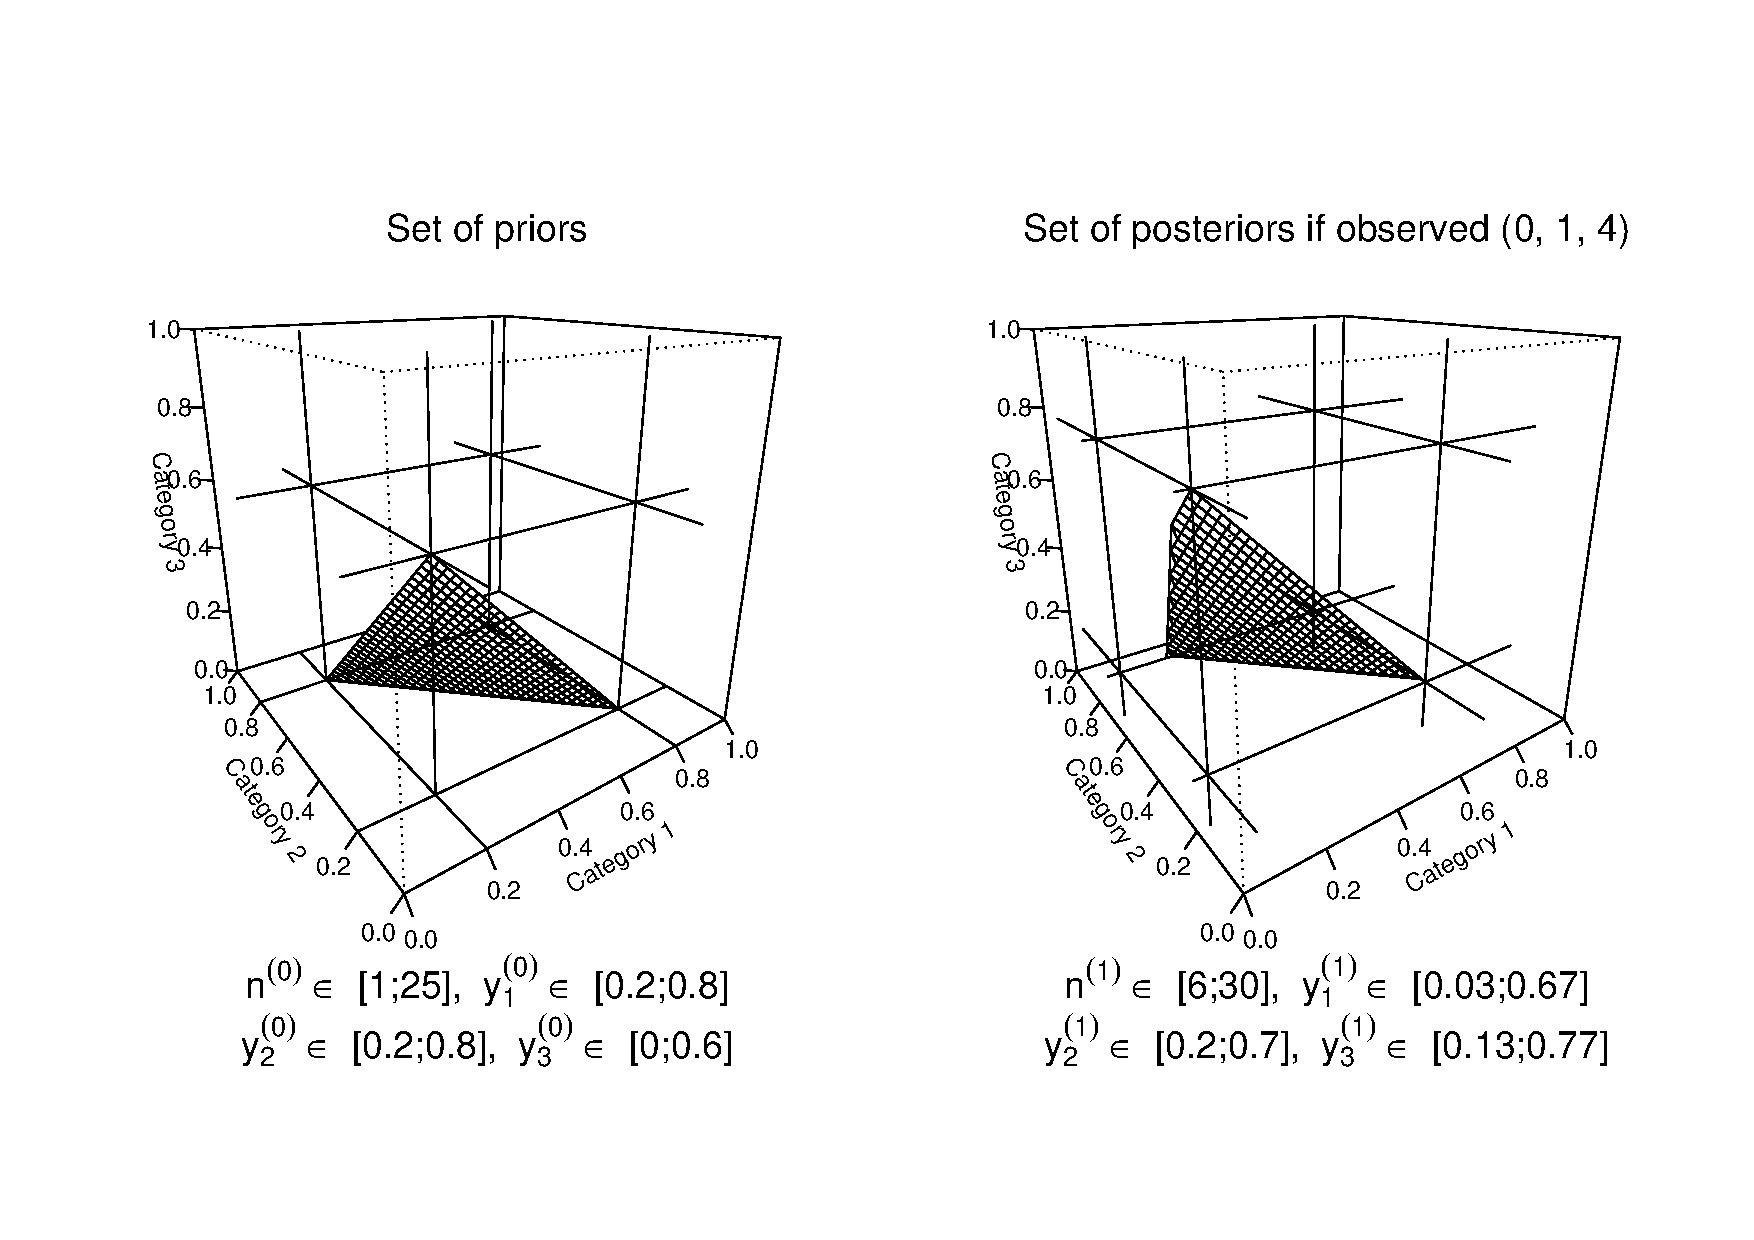
\includegraphics[trim = 150mm 25mm  20mm 20mm, clip, width=0.33\textwidth]{fig/jstp-paper_idm_nvar_zeile2-081205}%
\hspace*{-1.2ex}%
\end{tabular}%
\caption[Generalised \ymodel\ for samples from $\mult(\btheta)$:
prior and posterior credal sets for data in accordance with and contrary to prior beliefs.]%
{Prior (left) and posterior (center, right) credal sets for samples from
$\mult(\btheta)$ in accordance with (center) and contrary to (right)
prior beliefs. As in Figure~\ref{fig:nv-nvar-vertfu}, with \nymodel s
the sets differ in size according to the degree of prior-data conflict
induced by the observations.
}
\label{fig:idm-nvar-nopdc}
\end{figure}


\begin{example}[Dirichlet-Multinomial model, continued]
\label{ex:jstp-8}
For the Dirichlet-Multinomial model (Examples~\ref{ex:ymodel-idm} and \ref{ex:jstp-6}),
the behavior of the \nymodel\ is visualized in Figure~\ref{fig:idm-nvar-nopdc}. Here, the same set
of main parameters as in Figure~\ref{fig:idm-nfest-nopdc} is updated, leading
to plane cutouts (symbolising posterior parameter sets) that
differ not only in location as before, but also in size (and shape) for the
two cases. For the center graph, prior assumptions on the category
probabilities are in accordance with the observations 3, 2 and 0
for category one, two, and three, respectively, and thus the
posterior plane cutout is a subset of the prior plane. In
contrast, when observations 0, 1, and 4 are made, being in
conflict with the prior assumptions for category one and three,
the resulting posterior parameter intervals for those two
categories do actually get wider, as can be seen in the right
graph, and thus, inference drawn in this case is more cautious.
\end{example}

\begin{figure} %trim = l b r t
%\includegraphics[height=0.99\textwidth,angle=-90,bb = 20 15 575 825]{fig/jstp-paper_nv_nvar_HPD_n-infty_081201.ps}%
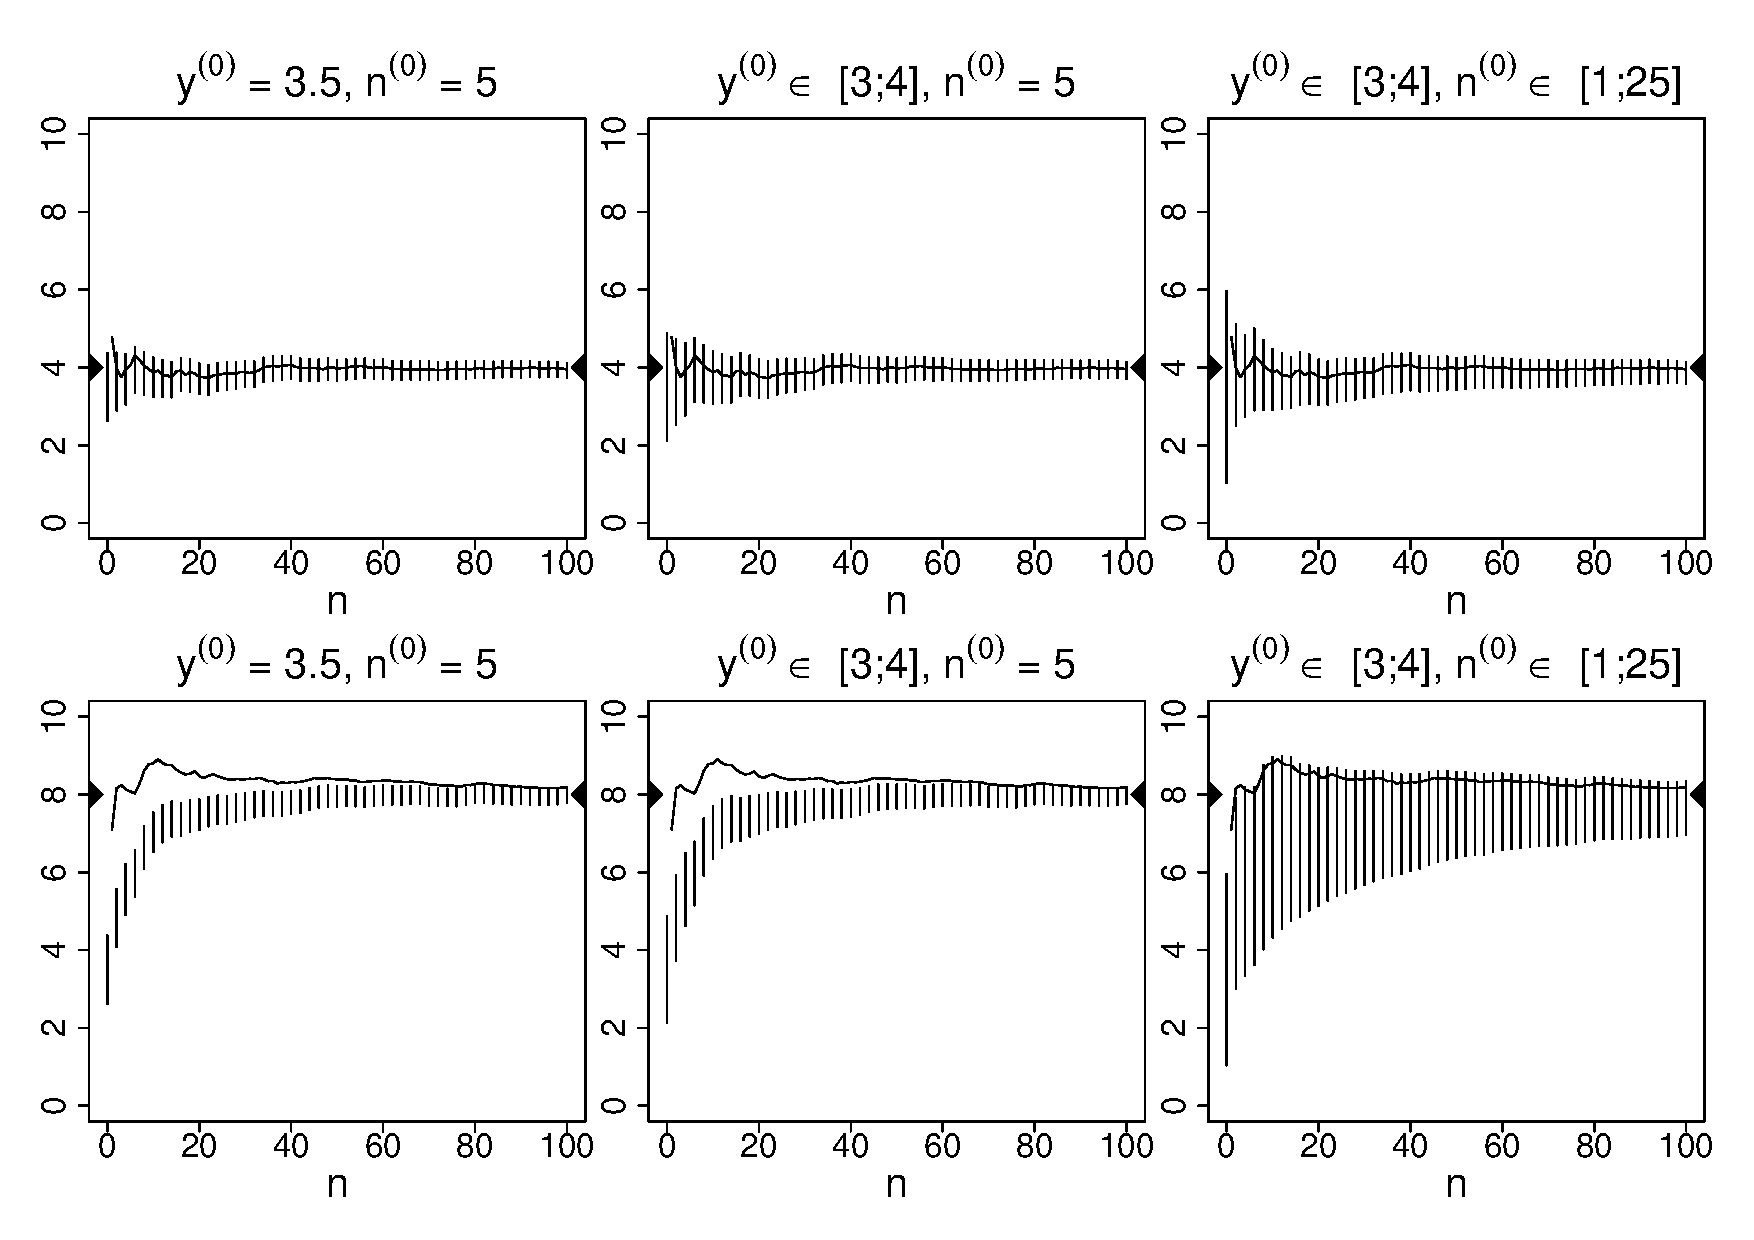
\includegraphics[trim = 5mm 5mm 5mm 5mm, clip, width=\textwidth]{fig/jstp-paper_nv_nvar_HPD_n-infty_081201}%
\caption[Comparison of (unions of) HPD intervals based on a single prior,
an \ymodel\ and a \nymodel.]%
{(Unions of) 95\%-posterior HD intervals (vertical lines) for
observations in accordance (upper row, drawn from $\mbox{N}(4,1)$)
and in conflict (lower row, drawn from $\mbox{N}(8,1)$) with prior assumptions
based on a single prior (left), an \ymodel\ (center) and a \nymodel\ (right)
in dependence on the sample size $n$. The development of the sample mean is
indicated by the wiggly line. Through the averaging, the HD intervals in the
lower left and center graph are not enlarged but only shifted and thus do not cover the sample mean.}
\label{fig:nv-nvar-kinfty}
\end{figure}

\begin{example}[Larger sample sizes]
\label{ex:jstp-9}
Sufficiently precise inference can be drawn nevertheless when the sample
size gets much larger with respect to the prior strength, giving
data more weight than the prior guess. When no prior-data conflict
occurs, the imprecision obtained with \nymodel s is not
substantially larger than obtained with \ymodel s or even with a
classical, precise prior. These three model classes are compared by means
of the Normal-Normal model (Examples~\ref{ex:ymodel-nv}, \ref{ex:jstp-7} and \ref{ex:jstp-7})
in Figure~\ref{fig:nv-nvar-kinfty}, where the first
column gives posterior HD (further denoted by HPD) intervals for a
precise prior, the second column unions of HPD intervals for the
\ymodel, and the third column unions of HPD intervals for the
\nymodel, in all three cases drawn as vertical black lines for
sample sizes $n=2,4,6,\ldots,100$.

In the upper row, these prior models are updated successively with
observations drawn from a $\norm(4,1)$ being in accordance with the prior assumptions,
whereas for the lower row, observations in conflict with the prior
assumptions were simulated by observations drawn from a $\norm(8,1)$.
In the upper row, the (unions of)
intervals tend to the sample mean indicated by the wiggly line
more or less uniformly for all three models. Naturally, the most
precise prior gives the most precise posterior inferences, but the
HPD interval lengths do not differ excessively between the model classes, especially
when the sample size $n$ approaches $100$.

The lower row demonstrates the deficiency that the classical and
the \ymodel\ unfortunately share. For them, observations confronting
the prior assumptions lead only to an adjustment in location of
the intervals through the averaging, but not in their length, giving
a false certainty in posterior inference. Here, the \nymodel\ is
more truthful to the character of the situation, giving very wide
unions of HPD intervals for low sample sizes covering both the a priori
assumed range and the sample mean. With growing sample size, more
confidence is given to the data, and thus, the unions of HPD intervals
tend the more to the sample mean the larger the sample gets.
\end{example}


\subsection{Concluding Remarks}
\label{sec:6-gw-071216}

***change it or leave it? draw links to other chapters and sections?***

In this ***paper***, we considered generalised Bayesian inference
in a wide class of imprecise probability models. We first
demonstrated that, in their originally proposed form, these models
do not react to prior-data conflict and so do not utilise
the full expressive power of imprecise probabilities. We
extended these models such that the natural relationship between
knowledge and imprecision is reestablished: the higher the
discrepancy between prior assumptions and sample observations, the
more cautious the posterior inference. We compare the previous
modelling and our extension in two running examples covering two
widely used situations, inference from a scaled normal and
from a multinomial distribution, corroborating that our extension
shows promising behavior.

Further research will start with a more detailed study of
the behavior of the proposed model, also taking into consideration
that it may have some problems with dealing with very extreme
degrees of conflict. Then careful attention should also be paid to
other approaches for generalised Bayesian inference in exponential
families \parencite{1993:coolen, 1997:boratynska} under prior data
conflict, as well as to a thorough comparison of the inference
developed here with the discretisation-based models considered by
\textcite{2005:whitcomb}, and with the approaches of \textcite{1991:pericchi}
and \textcite{1994:coolen}, who use different prior classes.

Far beyond these further developments, it should well be
remembered that this ***paper*** consciously confined the whole
argumentation to a certain Bayesian setting: we studied how far
one can go \emph{if} one relies strictly on the generalised Bayes
rule, transferring sets of priors to sets of posteriors element by
element via Bayes rule. Alternative learning
rules, including the approaches enumerated at Section~\ref{sec:jstp-intro},% %***paper intro*** %\ref{sec:intro},
\footnote{See also the critique regarding the Generalised Bayes' Rule in Section~\ref{sec:updating}.}
could prove very important as, to use one of the referees'
felicitous words, ``Bayesian methods cannot allow for surprise, the same is
true for robustified or generalised Bayesian methods, although these
may hide this shortcoming better. One could argue, therefore, that
they cannot be used to represent learning.''

\subsubsection*{Acknowledgements}
The authors would like to thank two anonymous referees for their very stimulating comments.



%\clearpage


\section{***The \texttt{luck} Package} %***Software***}
\label{sec:luck}

seperate section, take short description from abstract for ISIPTA'09 poster?


%\section{***Isipta'07 paper?***}

%***I would prefer not to include this, or just give a short summary of the contents.***



  \section{On Prior-Data Conflict in Predictive Bernoulli Inferences}
\label{sec:isipta11}

This section reproduces the work
``On Prior-Data Conflict in Predictive Bernoulli Inferences'',
published as a peer-reviewed contribution to
\emph{ISIPTA'11: Proceedings of the Seventh International Symposium on
Imprecise Probabilities: Theories and Applications} \parencite{Walter2011a}.
As such, it is reproduced here almost verbatim,
except for some minor shortenings, especially in the Introduction (Section~\ref{sec:isipta11-intro}),
and the addition of some comments and footnotes linking this work to other parts of this thesis.
Furthermore, the notation was changed slightly to assure consistency with the rest of the material presented in this thesis.
Specifically, the success probability in Bernoulli trials is denoted by $\theta$ instead of $p$.

%***with Frank's weighting model!***
\subsubsection*{Abstract}
%***abstract***

By its capability to deal with the multidimensional nature of
uncertainty, imprecise probability provides a powerful methodology
to sensibly handle \pdc\ in Bayesian inference. When there is
strong conflict between sample observations and prior knowledge, the posterior model should be more imprecise
than in the situation of mutual agreement or compatibility. Focusing
presentation on the prototypical example of Bernoulli
trials, we discuss the ability of different approaches to deal with \pdc.

We study a generalised Bayesian setting, including Walley's Imprecise Beta-Binomial model
and his extension to handle prior data conflict (called pdc-IBBM here).
We investigate alternative shapes of prior parameter sets, chosen in a way that shows improved
behaviour in the case of \pdc\ and their influence on the posterior predictive distribution.
Thereafter we present a new approach, consisting of an
imprecise weighting of two originally separate inferences, one of which is based on an informative
imprecise prior, whereas the other one is based on an uninformative imprecise prior. This approach
deals with \pdc\ in a fascinating way.
%***end of abstract***

\subsection{Introduction}
\label{sec:isipta11-intro}

Imprecise probability has shown to be a
powerful methodology to cope with the multidimensional nature of
uncertainty (see the discussion in Sections~\ref{sec:ip-intro} and \ref{sec:motivation}).
Imprecision allows the quality of information, on which probability statements are
based, to be modeled. Well supported knowledge is expressed by comparatively
precise models, while highly imprecise (or even vacuous) models reflect scarce (or no) knowledge
on probabilities. This flexible, multidimensional perspective on uncertainty
modeling has intensively been utilized in generalised Bayesian
inference to overcome the criticism of the arbitrariness of
the choice of single prior distributions in traditional Bayesian inference.%
\footnote{%See the basic discussion of the Bayesian approach to statistical inference in Section~\ref{sec:bayes-inference},
This criticism, subsumed by \textcite[\S 5]{1991:walley} as the ``dogma of precision'',
is discussed more detailed in Section~\ref{sec:motivation:bayesian}.}
In addition, only imprecise probability models react reliably to the presence of
\pdc, i.e.\ situations  where ``the prior [places] its mass primarily on
distributions in the sampling model for which the observed data is
surprising'' \parencite[p.~894]{2006:evans}. Lower and upper probabilities%
\footnote{See Section~\ref{sec:ip-main} for a short exposition of lower and upper previsions,
and related mathematical tools for handling uncertainty in statistical inference.}
allow a specific reaction to \pdc, and offer reasonable inferences if the analyst wishes to
stick to his prior assumptions: starting with the same level of ambiguity in the prior
specification, wide posterior intervals can
reflect conflict between prior and data, while
no \pdc\ will lead to narrow intervals.%
\footnote{See the discussions in Sections~\ref{sec:motivation:pdc} and \ref{sec:pdc-sensitivity},
and the ***work*** on \pdc\ in Section~\ref{sec:jstp}.}
Ideally, the model could provide an extra `bonus' of precision if prior %specifications had been `spot on'.
assumptions are very strongly supported by the data.
Such a model would have the advantage
of (relatively) precise answers when the data confirm prior assumptions,
while still rendering more cautionary answers in the case of \pdc,
thus leading to cautious inferences if, and only if, caution is needed.

Although \textcite[p.~6]{1991:walley} explicitly emphasizes this possibility to
express prior-data conflict as one of the main motivations for imprecise probability,
it has received surprisingly little attention. Rare exceptions include two short sections in \textcite[p.~6 and \S 5.4]{1991:walley}
and the papers by \textcite{1991:pericchi}, \textcite{1994:coolen} and
\textcite{2005:whitcomb}. The popular IDM \parencite{1996:walley::idm, 2009:bernard}
and its generalisation to exponential families \parencite{2005:quaeghebeurcooman} do not reflect prior-data conflict.
\textcite[see Section~\ref{sec:jstp}]{Walter2009a} used the basic ideas of \textcite[\S 5.4]{1991:walley} to extend the approach of
\textcite{2005:quaeghebeurcooman} to models that show sensitivity to \pdc.

In this work, a deeper investigation of the issue of \pdc\ is undertaken,
focusing on the prototypic special case of predictive inference in Bernoulli trials:%
\footnote{See also the discussion of the Beta-Binomial model in Section~\ref{sec:beta-binom},
and the imprecise Dirichlet-Multinomial model discussed in several examples in Section~\ref{sec:jstp}.}
We are interested in the posterior predictive
probability for the event that a future Bernoulli random quantity
will have the value $1$, also called a `success'. This event is not
explicitly included in the notation, i.e.\ we simply denote its lower
and upper probabilities by $\Pl$ and $\Pu$, respectively. This future Bernoulli random
quantity is assumed to be exchangeable with the Bernoulli random
quantities whose observations are summarised in the data, consisting
of the number $n$ of observations and the number $s$ of these that are
successes. In our analysis of this model, we
will often treat $s$ as a a real-valued observation in $[0,n]$,
keeping in mind that in reality it can only take %on
integer values, but the continuous representation is convenient for
our discussions, in particular in our predictive probability plots (PPP),
where for given $n$, $\Pl$ and $\Pu$ are discussed as functions of $s$.

\medskip

Section~\ref{sec:ibbm-framework} describes a general framework for
generalised Bayesian inference in this setting. The method presented in \textcite[\S 5.4.3]{1991:walley},
called `pdc-IBBM' in this paper, is considered in detail in Section~\ref{sec:ibbm-walley}
and we show that its reaction to \pdc\ can be improved
by suitable modifications of the underlying imprecise
priors. A basic proposal along these lines is discussed in
Section~\ref{sec:othershapes}, with further alternatives
sketched in Section~\ref{sec:ibbm-resume}.
Section~\ref{sec:weightedinf} addresses the problem of \pdc\ from a
completely different angle. There, we combine two originally separate
inferences, one based on an informative imprecise prior and one
on an uninformative imprecise prior, by an imprecise weighting
scheme. The ***paper*** concludes with a brief comparison of the different
approaches in Section~\ref{sec:insights}.


\subsection{Imprecise Beta-Binomial Models}
\label{sec:ibbm}

\subsubsection{The Framework}
\label{sec:ibbm-framework}

%***change notation for success probability from $p$ to $\theta$!!!***

The traditional Bayesian approach for our basic problem is the Beta-Binominal model, which expresses prior
beliefs about the probability $\theta$ of observing a `success' by a Beta
distribution. With\footnote{Our notation relates to
Walley's \parencite*{1991:walley} as $\nz \leftrightarrow s_0$, $\yz \leftrightarrow t_0$.}
$f(\theta\mid\nz, \yz) \propto \theta^{\nz\yz -1} (1-\theta)^{\nz(1-\yz)-1}$,
$\yz = \E[\theta\mid\nz,\yz]$ can be interpreted as prior guess of
$\theta$, while $\nz$ governs the concentration of
probability mass around $\yz$, also known as `pseudo counts' or
`prior strength'.\footnote{As in previous parts of the thesis, ${}\uz$ denotes prior parameters; ${}\un$ posterior parameters.}
These denominations are due to the
role of $\nz$ in the update step: With $s$ successes in $n$ draws observed, the
posterior parameters are\footnote{Compare to Section~\ref{sec:regularconjugates},
Equation~\eqref{eq:canonicalupdate}:
the model is prototypic for conjugate Bayesian
analysis in canonical exponential families, for which updating
of the parameters $\nz$ and $\yz$ can be
written as \eqref{equ:update-nn-yn-precise}.} %\vspace*{-1.3ex}
\begin{align}\label{equ:update-nn-yn-precise}
%\nn &= \nz + n, & \yn &= \frac{\nz}{\nz + n}\,\yz + \frac{n}{\nz + n}\, \frac{s}{n}.
\nn &= \nz + n, & \yn &= \frac{\nz\yz + s}{\nz + n}\,.
\end{align}
Thus $\yn$ is a weighted average of the prior parameter $\yz$ and
the sample proportion $s/n$, and potential prior data conflict is simply averaged out.

Overcoming the dogma of precision, formulating generalised Bayes
updating in this setting is straightforward. By Walley's Generalised
Bayes' Rule \parencite[\S 6]{1991:walley}%
\footnote{For more details on the Generalised Bayes' Rule and the generalised Bayesian inference procedure,
see Sections~\ref{sec:gbr} and \ref{sec:imprecisebayes}, respectively.}
the imprecise prior $\MZ$, described by convex sets of precise prior distributions,
is updated to the imprecise posterior $\MN$ obtained by updating $\MZ$ element-wise.
In particular, the convenient conjugate analysis used above can be extended:%
\footnote{See the discussion of the general framework for generalised Bayesian inference
based on sets of conjugate priors in Section~\ref{sec:basicsetting}.}
One specifies a prior parameter set
$\PZ$ of $(\nz,\yz)$ values and takes as imprecise
prior the set $\MZ$ consisting of  all convex mixtures of Beta
priors with $(\nz, \yz) \in \PZ$. In this sense, the set of Beta
priors corresponding to $\PZ$ gives the set of extreme points for
the actual convex set of priors $\MZ$. Updating $\MZ$ with the
Generalised Bayes' Rule results in the convex set $\MN$ of posterior
distributions, that conveniently can be obtained by taking the
convex hull of the set of Beta posteriors, which in turn are defined
by the set of updated parameters
$\PN = \{(\nn,\yn) \mid (\nz, \yz) \in \PZ\}$.
This relationship between the sets $\PZ$ and $\PN$ and the sets $\MZ$
and $\MN$ will allow us to discuss different models $\MZ$ and $\MN$ by depicting
the corresponding parameter sets $\PZ$ and $\PN$. When interpreting our results,
care will be needed with respect to convexity. Although
$\MZ$ and $\MN$ are convex, the parameter sets $\PZ$ and $\PN$
generating them need not necessarily be so. %convex.
Indeed, convexity of the parameter set is not necessarily preserved in the update
step: Convexity of $\PZ$ does not imply convexity of $\PN$.

Throughout, we are interested in the posterior predictive
probability $[\Pl,\Pu]$ for the event that a
future draw is a success. In the Beta-Bernoulli model, this
probability is equal to $\yn$, and we get%
%\footnote{\textcite{2005:quaeghebeurcooman}, \textcite{Walter2009a}, and \textcite{Walter2007a} use the prototypical character of
%\eqref{equ:update-nn-yn-precise} underlying \eqref{equ:General-Pl} and
%\eqref{equ:General-Pu} to generalise this inference to models based on canonical exponential families.
%See Section~\ref{sec:generalmodel} and \ref{sec:jstp}. ***leave this out here??***}
%
\begin{align}
\Pl = \ynl &:= \min_{\PN} \yn = \min_{\PZ} \frac{\nz\yz + s}{\nz +n}\,, \label{equ:General-Pl}\\
%           & = \min_{\nz \in [\nzl, \nzu]} \frac{\nz\yzl + s}{\nz +n} & &\text{and} \nonumber\\
\Pu = \ynu &:= \max_{\PN} \yn = \max_{\PZ} \frac{\nz\yz + s}{\nz +n}\,. \label{equ:General-Pu}
%           & = \max_{\nz \in [\nzl, \nzu]} \frac{\nz\yzu + s}{\nz +n}. \nonumber
\end{align}
%\begin{align*}
%\Pl(S^* = 1\mid s) &= \min_{(\nn, \yn) \in \PN} \yn \quad \text{and}\\
%\Pu(S^* = 1\mid s) &= \max_{(\nn, \yn) \in \PN} \yn.
%\end{align*}
%$\Pl(S^* = 1\mid s) = \min_{(\nn, \yn) \in \PN} \yn$ and
%$\Pu(S^* = 1\mid s) = \max_{(\nn, \yn) \in \PN} \yn$.


\subsubsection{Walley's pdc-IBBM}
\label{sec:ibbm-walley}

Special imprecise probability models are now obtained by specific
choices of $\PZ$. If one fixes $\nz$ and varies $\yz$ in an interval $[\yzl,\yzu]$,
Walley's \parencite*[\S 5.3]{1991:walley} model with learning parameter $\nz$ is obtained, which typically
is used in its near-ignorance form $[\yzl, \yzu] \to (0,1)$,
denoted as the imprecise Beta (Binomal/Bernoulli) model (IBBM)%
\footnote{We use `IBBM' also for the model with prior information.},
which is a special case of the popular Imprecise Dirichlet (Multinomial) Model
\parencite{1996:walley::idm,1999:walleybernard}. Unfortunately, in this basic form with fixed $\nz$, the model is
insensitive to prior-data conflict \parencite[p.~263, see Section~\ref{section:fixednschlecht}]{Walter2009a}.
\textcite[\S 5.4]{1991:walley} therefore generalised this
model by additionally varying $\nz$. In his extended model,
called \emph{pdc-IBBM} in this work, the set of priors is defined via the
set of prior parameters $\PZ = [\nzl, \nzu] \times [\yzl, \yzu]$,
being a two-dimensional interval, or a rectangle set.
Studying inference in this model, it is important to note that the set of posterior parameters
%$\PN = \{(\nn,\yn) \mid [\nzl, \nzu] \times [\yzl, \yzu]\}$
%$\PN = \{(\nn,\yn) \mid (\nz, \yz) \in \PZero\}$ defining the set
%of ***vertex*** posterior distributions is not rectangular anymore.
$\PN$ is not rectangular anymore. The resulting shapes are illustrated in Figure~\ref{fig:spot-banana}: For the
prior set $\PZ = [1, 5 ] \times  [0.4, 0.7]$---thus assuming a priori the
fraction of successes to be between 40\% and 70\% and rating these assumptions
with at least $1$ and at most $5$ pseudo observations---the resulting posterior parameter sets $\PN$
are shown for data consisting of 3 successes in 6 draws (left) and with all 6 draws successes (right). %***TPDA***. On the right, ***PDC***.
We call the left shape \emph{spotlight}, and the right shape
\emph{banana}. In both graphs, the elements of $\PN$ yielding
%the minimal and maximal $\yn$, $\ynl = \LE[p\mid s]$ and $\ynu = \UE[p\mid s]$,
$\ynl$ and $\ynu$, and thus $\Pl$ and $\Pu$,
are marked with a circle.

%\begin{verbatim}
\begin{figure}%[t]
\begin{tikzpicture}
%\pgftransformscale{0.475}
\pgftransformscale{0.04}
%\include{simpleEx.tex}
% Created by tikzDevice version 0.5.0 on 2011-02-28 18:34:50
\begin{scope}
\path[clip] (  0.00,  0.00) rectangle (397.48,216.81);
\definecolor[named]{fillColor}{rgb}{0.88,0.08,0.52}
\definecolor[named]{drawColor}{rgb}{0.00,0.00,0.00}

\draw[color=drawColor,line cap=round,line join=round,fill opacity=0.00,] ( 60.43, 49.20) -- (191.11, 49.20);

\draw[color=drawColor,line cap=round,line join=round,fill opacity=0.00,] ( 60.43, 49.20) -- ( 60.43, 43.20);

\draw[color=drawColor,line cap=round,line join=round,fill opacity=0.00,] ( 93.10, 49.20) -- ( 93.10, 43.20);

\draw[color=drawColor,line cap=round,line join=round,fill opacity=0.00,] (125.77, 49.20) -- (125.77, 43.20);

\draw[color=drawColor,line cap=round,line join=round,fill opacity=0.00,] (158.44, 49.20) -- (158.44, 43.20);

\draw[color=drawColor,line cap=round,line join=round,fill opacity=0.00,] (191.11, 49.20) -- (191.11, 43.20);

\node[color=drawColor,anchor=base,inner sep=0pt, outer sep=0pt, scale=  0.90] at ( 60.43, 25.20) {7%
};

\node[color=drawColor,anchor=base,inner sep=0pt, outer sep=0pt, scale=  0.90] at ( 93.10, 25.20) {8%
};

\node[color=drawColor,anchor=base,inner sep=0pt, outer sep=0pt, scale=  0.90] at (125.77, 25.20) {9%
};

\node[color=drawColor,anchor=base,inner sep=0pt, outer sep=0pt, scale=  0.90] at (158.44, 25.20) {10%
};

\node[color=drawColor,anchor=base,inner sep=0pt, outer sep=0pt, scale=  0.90] at (191.11, 25.20) {11%
};

\draw[color=drawColor,line cap=round,line join=round,fill opacity=0.00,] ( 55.20, 66.64) -- ( 55.20,165.70);

\draw[color=drawColor,line cap=round,line join=round,fill opacity=0.00,] ( 55.20, 66.64) -- ( 49.20, 66.64);

\draw[color=drawColor,line cap=round,line join=round,fill opacity=0.00,] ( 55.20, 91.40) -- ( 49.20, 91.40);

\draw[color=drawColor,line cap=round,line join=round,fill opacity=0.00,] ( 55.20,116.17) -- ( 49.20,116.17);

\draw[color=drawColor,line cap=round,line join=round,fill opacity=0.00,] ( 55.20,140.93) -- ( 49.20,140.93);

\draw[color=drawColor,line cap=round,line join=round,fill opacity=0.00,] ( 55.20,165.70) -- ( 49.20,165.70);

\node[rotate= 90.00,color=drawColor,anchor=base,inner sep=0pt, outer sep=0pt, scale=  0.90] at ( 43.20, 66.64) {0.5%
};

\node[rotate= 90.00,color=drawColor,anchor=base,inner sep=0pt, outer sep=0pt, scale=  0.90] at ( 43.20, 91.40) {0.6%
};

\node[rotate= 90.00,color=drawColor,anchor=base,inner sep=0pt, outer sep=0pt, scale=  0.90] at ( 43.20,116.17) {0.7%
};

\node[rotate= 90.00,color=drawColor,anchor=base,inner sep=0pt, outer sep=0pt, scale=  0.90] at ( 43.20,140.93) {0.8%
};

\node[rotate= 90.00,color=drawColor,anchor=base,inner sep=0pt, outer sep=0pt, scale=  0.90] at ( 43.20,165.70) {0.9%
};

\draw[color=drawColor,line cap=round,line join=round,fill opacity=0.00,] ( 55.20, 49.20) --
	(196.34, 49.20) --
	(196.34,185.61) --
	( 55.20,185.61) --
	( 55.20, 49.20);
\end{scope}
\begin{scope}
\path[clip] (  0.00,  0.00) rectangle (198.74,216.81);
\definecolor[named]{fillColor}{rgb}{0.88,0.08,0.52}
\definecolor[named]{drawColor}{rgb}{0.00,0.00,0.00}

\node[color=drawColor,anchor=base,inner sep=0pt, outer sep=0pt, scale=  1.00] at (125.77,  1.20) {$\nn$%
};

\node[rotate= 90.00,color=drawColor,anchor=base,inner sep=0pt, outer sep=0pt, scale=  1.00] at ( 19.20,117.41) {$\yn$%
};
\end{scope}
\begin{scope}
\path[clip] ( 55.20, 49.20) rectangle (196.34,185.61);
\definecolor[named]{fillColor}{rgb}{0.88,0.08,0.52}
\definecolor[named]{drawColor}{rgb}{0.00,0.00,0.00}
\definecolor[named]{fillColor}{rgb}{0.75,0.75,0.75}

\draw[color=drawColor,line cap=round,line join=round,fill=fillColor,] ( 60.43, 63.10) --
	( 61.75, 62.98) --
	( 63.07, 62.85) --
	( 64.39, 62.74) --
	( 65.71, 62.62) --
	( 67.03, 62.50) --
	( 68.35, 62.39) --
	( 69.67, 62.27) --
	( 70.99, 62.16) --
	( 72.31, 62.05) --
	( 73.63, 61.94) --
	( 74.95, 61.83) --
	( 76.27, 61.72) --
	( 77.59, 61.62) --
	( 78.91, 61.51) --
	( 80.23, 61.41) --
	( 81.55, 61.30) --
	( 82.87, 61.20) --
	( 84.19, 61.10) --
	( 85.51, 61.00) --
	( 86.83, 60.90) --
	( 88.15, 60.80) --
	( 89.47, 60.71) --
	( 90.79, 60.61) --
	( 92.11, 60.51) --
	( 93.43, 60.42) --
	( 94.75, 60.33) --
	( 96.07, 60.23) --
	( 97.39, 60.14) --
	( 98.71, 60.05) --
	(100.03, 59.96) --
	(101.35, 59.88) --
	(102.67, 59.79) --
	(103.99, 59.70) --
	(105.31, 59.61) --
	(106.63, 59.53) --
	(107.95, 59.45) --
	(109.27, 59.36) --
	(110.59, 59.28) --
	(111.91, 59.20) --
	(113.23, 59.12) --
	(114.55, 59.03) --
	(115.87, 58.96) --
	(117.19, 58.88) --
	(118.51, 58.80) --
	(119.83, 58.72) --
	(121.15, 58.64) --
	(122.47, 58.57) --
	(123.79, 58.49) --
	(125.11, 58.42) --
	(126.43, 58.34) --
	(127.75, 58.27) --
	(129.07, 58.20) --
	(130.39, 58.12) --
	(131.71, 58.05) --
	(133.03, 57.98) --
	(134.35, 57.91) --
	(135.67, 57.84) --
	(136.99, 57.77) --
	(138.31, 57.70) --
	(139.63, 57.64) --
	(140.95, 57.57) --
	(142.27, 57.50) --
	(143.59, 57.44) --
	(144.91, 57.37) --
	(146.23, 57.31) --
	(147.55, 57.24) --
	(148.87, 57.18) --
	(150.19, 57.11) --
	(151.51, 57.05) --
	(152.83, 56.99) --
	(154.15, 56.93) --
	(155.47, 56.87) --
	(156.79, 56.80) --
	(158.11, 56.74) --
	(159.43, 56.68) --
	(160.75, 56.62) --
	(162.07, 56.57) --
	(163.39, 56.51) --
	(164.71, 56.45) --
	(166.03, 56.39) --
	(167.35, 56.33) --
	(168.67, 56.28) --
	(169.99, 56.22) --
	(171.31, 56.17) --
	(172.63, 56.11) --
	(173.95, 56.06) --
	(175.27, 56.00) --
	(176.59, 55.95) --
	(177.91, 55.89) --
	(179.23, 55.84) --
	(180.55, 55.79) --
	(181.87, 55.73) --
	(183.19, 55.68) --
	(184.51, 55.63) --
	(185.83, 55.58) --
	(187.15, 55.53) --
	(188.47, 55.48) --
	(189.79, 55.43) --
	(191.11, 55.38) --
	(191.11, 89.15) --
	(189.79, 89.05) --
	(188.47, 88.95) --
	(187.15, 88.85) --
	(185.83, 88.75) --
	(184.51, 88.64) --
	(183.19, 88.54) --
	(181.87, 88.44) --
	(180.55, 88.33) --
	(179.23, 88.23) --
	(177.91, 88.12) --
	(176.59, 88.01) --
	(175.27, 87.90) --
	(173.95, 87.79) --
	(172.63, 87.68) --
	(171.31, 87.57) --
	(169.99, 87.46) --
	(168.67, 87.35) --
	(167.35, 87.24) --
	(166.03, 87.12) --
	(164.71, 87.01) --
	(163.39, 86.89) --
	(162.07, 86.77) --
	(160.75, 86.66) --
	(159.43, 86.54) --
	(158.11, 86.42) --
	(156.79, 86.30) --
	(155.47, 86.18) --
	(154.15, 86.05) --
	(152.83, 85.93) --
	(151.51, 85.80) --
	(150.19, 85.68) --
	(148.87, 85.55) --
	(147.55, 85.42) --
	(146.23, 85.29) --
	(144.91, 85.16) --
	(143.59, 85.03) --
	(142.27, 84.90) --
	(140.95, 84.77) --
	(139.63, 84.63) --
	(138.31, 84.50) --
	(136.99, 84.36) --
	(135.67, 84.22) --
	(134.35, 84.08) --
	(133.03, 83.94) --
	(131.71, 83.80) --
	(130.39, 83.66) --
	(129.07, 83.51) --
	(127.75, 83.37) --
	(126.43, 83.22) --
	(125.11, 83.07) --
	(123.79, 82.92) --
	(122.47, 82.77) --
	(121.15, 82.62) --
	(119.83, 82.46) --
	(118.51, 82.31) --
	(117.19, 82.15) --
	(115.87, 82.00) --
	(114.55, 81.84) --
	(113.23, 81.67) --
	(111.91, 81.51) --
	(110.59, 81.35) --
	(109.27, 81.18) --
	(107.95, 81.02) --
	(106.63, 80.85) --
	(105.31, 80.68) --
	(103.99, 80.50) --
	(102.67, 80.33) --
	(101.35, 80.15) --
	(100.03, 79.98) --
	( 98.71, 79.80) --
	( 97.39, 79.62) --
	( 96.07, 79.44) --
	( 94.75, 79.25) --
	( 93.43, 79.06) --
	( 92.11, 78.88) --
	( 90.79, 78.69) --
	( 89.47, 78.49) --
	( 88.15, 78.30) --
	( 86.83, 78.10) --
	( 85.51, 77.91) --
	( 84.19, 77.71) --
	( 82.87, 77.50) --
	( 81.55, 77.30) --
	( 80.23, 77.09) --
	( 78.91, 76.89) --
	( 77.59, 76.67) --
	( 76.27, 76.46) --
	( 74.95, 76.25) --
	( 73.63, 76.03) --
	( 72.31, 75.81) --
	( 70.99, 75.58) --
	( 69.67, 75.36) --
	( 68.35, 75.13) --
	( 67.03, 74.90) --
	( 65.71, 74.67) --
	( 64.39, 74.43) --
	( 63.07, 74.20) --
	( 61.75, 73.95) --
	( 60.43, 73.71) --
	cycle;
\end{scope}
\begin{scope}
\path[clip] (  0.00,  0.00) rectangle (397.48,216.81);
\definecolor[named]{fillColor}{rgb}{0.88,0.08,0.52}
\definecolor[named]{drawColor}{rgb}{0.00,0.00,0.00}

\node[color=drawColor,anchor=base,inner sep=0pt, outer sep=0pt, scale=  1.00] at (125.77,203.61) {$s = 3$, $n=6$%
};
\end{scope}
\begin{scope}
\path[clip] ( 55.20, 49.20) rectangle (196.34,185.61);
\definecolor[named]{fillColor}{rgb}{0.88,0.08,0.52}
\definecolor[named]{drawColor}{rgb}{0.00,0.00,0.00}

\draw[color=drawColor,line cap=round,line join=round,fill opacity=0.00,] (191.11, 55.38) circle (  3.38);

\draw[color=drawColor,line cap=round,line join=round,fill opacity=0.00,] (191.11, 89.15) circle (  3.38);
\end{scope}
\begin{scope}
\path[clip] (253.94, 49.20) rectangle (395.08,185.61);
\definecolor[named]{fillColor}{rgb}{0.88,0.08,0.52}
\end{scope}
\begin{scope}
\path[clip] (  0.00,  0.00) rectangle (397.48,216.81);
\definecolor[named]{fillColor}{rgb}{0.88,0.08,0.52}
\definecolor[named]{drawColor}{rgb}{0.00,0.00,0.00}

\draw[color=drawColor,line cap=round,line join=round,fill opacity=0.00,] (259.17, 49.20) -- (389.86, 49.20);

\draw[color=drawColor,line cap=round,line join=round,fill opacity=0.00,] (259.17, 49.20) -- (259.17, 43.20);

\draw[color=drawColor,line cap=round,line join=round,fill opacity=0.00,] (291.84, 49.20) -- (291.84, 43.20);

\draw[color=drawColor,line cap=round,line join=round,fill opacity=0.00,] (324.51, 49.20) -- (324.51, 43.20);

\draw[color=drawColor,line cap=round,line join=round,fill opacity=0.00,] (357.19, 49.20) -- (357.19, 43.20);

\draw[color=drawColor,line cap=round,line join=round,fill opacity=0.00,] (389.86, 49.20) -- (389.86, 43.20);

\node[color=drawColor,anchor=base,inner sep=0pt, outer sep=0pt, scale=  0.90] at (259.17, 25.20) {7%
};

\node[color=drawColor,anchor=base,inner sep=0pt, outer sep=0pt, scale=  0.90] at (291.84, 25.20) {8%
};

\node[color=drawColor,anchor=base,inner sep=0pt, outer sep=0pt, scale=  0.90] at (324.51, 25.20) {9%
};

\node[color=drawColor,anchor=base,inner sep=0pt, outer sep=0pt, scale=  0.90] at (357.19, 25.20) {10%
};

\node[color=drawColor,anchor=base,inner sep=0pt, outer sep=0pt, scale=  0.90] at (389.86, 25.20) {11%
};

\draw[color=drawColor,line cap=round,line join=round,fill opacity=0.00,] (253.94, 66.64) -- (253.94,165.70);

\draw[color=drawColor,line cap=round,line join=round,fill opacity=0.00,] (253.94, 66.64) -- (247.94, 66.64);

\draw[color=drawColor,line cap=round,line join=round,fill opacity=0.00,] (253.94, 91.40) -- (247.94, 91.40);

\draw[color=drawColor,line cap=round,line join=round,fill opacity=0.00,] (253.94,116.17) -- (247.94,116.17);

\draw[color=drawColor,line cap=round,line join=round,fill opacity=0.00,] (253.94,140.93) -- (247.94,140.93);

\draw[color=drawColor,line cap=round,line join=round,fill opacity=0.00,] (253.94,165.70) -- (247.94,165.70);

\node[rotate= 90.00,color=drawColor,anchor=base,inner sep=0pt, outer sep=0pt, scale=  0.90] at (241.94, 66.64) {0.5%
};

\node[rotate= 90.00,color=drawColor,anchor=base,inner sep=0pt, outer sep=0pt, scale=  0.90] at (241.94, 91.40) {0.6%
};

\node[rotate= 90.00,color=drawColor,anchor=base,inner sep=0pt, outer sep=0pt, scale=  0.90] at (241.94,116.17) {0.7%
};

\node[rotate= 90.00,color=drawColor,anchor=base,inner sep=0pt, outer sep=0pt, scale=  0.90] at (241.94,140.93) {0.8%
};

\node[rotate= 90.00,color=drawColor,anchor=base,inner sep=0pt, outer sep=0pt, scale=  0.90] at (241.94,165.70) {0.9%
};

\draw[color=drawColor,line cap=round,line join=round,fill opacity=0.00,] (253.94, 49.20) --
	(395.08, 49.20) --
	(395.08,185.61) --
	(253.94,185.61) --
	(253.94, 49.20);
\end{scope}
\begin{scope}
\path[clip] (198.74,  0.00) rectangle (397.48,216.81);
\definecolor[named]{fillColor}{rgb}{0.88,0.08,0.52}
\definecolor[named]{drawColor}{rgb}{0.00,0.00,0.00}

\node[color=drawColor,anchor=base,inner sep=0pt, outer sep=0pt, scale=  1.00] at (324.51,  1.20) {$\nn$%
};

\node[rotate= 90.00,color=drawColor,anchor=base,inner sep=0pt, outer sep=0pt, scale=  1.00] at (217.94,117.41) {$\yn$%
};
\end{scope}
\begin{scope}
\path[clip] (253.94, 49.20) rectangle (395.08,185.61);
\definecolor[named]{fillColor}{rgb}{0.88,0.08,0.52}
\definecolor[named]{drawColor}{rgb}{0.00,0.00,0.00}
\definecolor[named]{fillColor}{rgb}{0.75,0.75,0.75}

\draw[color=drawColor,line cap=round,line join=round,fill=fillColor,] (259.17,169.24) --
	(260.49,168.51) --
	(261.81,167.78) --
	(263.13,167.07) --
	(264.45,166.36) --
	(265.77,165.66) --
	(267.09,164.97) --
	(268.41,164.29) --
	(269.73,163.61) --
	(271.05,162.95) --
	(272.37,162.29) --
	(273.69,161.63) --
	(275.01,160.99) --
	(276.33,160.35) --
	(277.65,159.71) --
	(278.97,159.09) --
	(280.29,158.47) --
	(281.61,157.86) --
	(282.93,157.25) --
	(284.25,156.65) --
	(285.57,156.05) --
	(286.89,155.47) --
	(288.21,154.89) --
	(289.53,154.31) --
	(290.85,153.74) --
	(292.17,153.17) --
	(293.49,152.62) --
	(294.81,152.06) --
	(296.13,151.52) --
	(297.45,150.97) --
	(298.77,150.44) --
	(300.09,149.91) --
	(301.41,149.38) --
	(302.73,148.86) --
	(304.05,148.34) --
	(305.37,147.83) --
	(306.69,147.32) --
	(308.01,146.82) --
	(309.33,146.33) --
	(310.65,145.83) --
	(311.97,145.35) --
	(313.29,144.86) --
	(314.61,144.38) --
	(315.93,143.91) --
	(317.25,143.44) --
	(318.57,142.98) --
	(319.89,142.51) --
	(321.21,142.06) --
	(322.53,141.60) --
	(323.85,141.16) --
	(325.17,140.71) --
	(326.49,140.27) --
	(327.81,139.83) --
	(329.13,139.40) --
	(330.45,138.97) --
	(331.77,138.55) --
	(333.09,138.12) --
	(334.41,137.71) --
	(335.73,137.29) --
	(337.05,136.88) --
	(338.37,136.47) --
	(339.69,136.07) --
	(341.01,135.67) --
	(342.33,135.27) --
	(343.65,134.88) --
	(344.97,134.49) --
	(346.30,134.10) --
	(347.62,133.72) --
	(348.94,133.34) --
	(350.26,132.96) --
	(351.58,132.58) --
	(352.90,132.21) --
	(354.22,131.84) --
	(355.54,131.48) --
	(356.86,131.12) --
	(358.18,130.76) --
	(359.50,130.40) --
	(360.82,130.05) --
	(362.14,129.70) --
	(363.46,129.35) --
	(364.78,129.00) --
	(366.10,128.66) --
	(367.42,128.32) --
	(368.74,127.98) --
	(370.06,127.65) --
	(371.38,127.31) --
	(372.70,126.99) --
	(374.02,126.66) --
	(375.34,126.33) --
	(376.66,126.01) --
	(377.98,125.69) --
	(379.30,125.37) --
	(380.62,125.06) --
	(381.94,124.75) --
	(383.26,124.44) --
	(384.58,124.13) --
	(385.90,123.82) --
	(387.22,123.52) --
	(388.54,123.22) --
	(389.86,122.92) --
	(389.86,156.69) --
	(388.54,156.84) --
	(387.22,156.99) --
	(385.90,157.14) --
	(384.58,157.30) --
	(383.26,157.45) --
	(381.94,157.61) --
	(380.62,157.76) --
	(379.30,157.92) --
	(377.98,158.08) --
	(376.66,158.24) --
	(375.34,158.40) --
	(374.02,158.56) --
	(372.70,158.72) --
	(371.38,158.89) --
	(370.06,159.06) --
	(368.74,159.22) --
	(367.42,159.39) --
	(366.10,159.56) --
	(364.78,159.73) --
	(363.46,159.91) --
	(362.14,160.08) --
	(360.82,160.26) --
	(359.50,160.43) --
	(358.18,160.61) --
	(356.86,160.79) --
	(355.54,160.97) --
	(354.22,161.15) --
	(352.90,161.34) --
	(351.58,161.52) --
	(350.26,161.71) --
	(348.94,161.90) --
	(347.62,162.09) --
	(346.29,162.28) --
	(344.97,162.48) --
	(343.65,162.67) --
	(342.33,162.87) --
	(341.01,163.07) --
	(339.69,163.27) --
	(338.37,163.47) --
	(337.05,163.67) --
	(335.73,163.88) --
	(334.41,164.08) --
	(333.09,164.29) --
	(331.77,164.50) --
	(330.45,164.72) --
	(329.13,164.93) --
	(327.81,165.15) --
	(326.49,165.37) --
	(325.17,165.59) --
	(323.85,165.81) --
	(322.53,166.03) --
	(321.21,166.26) --
	(319.89,166.49) --
	(318.57,166.72) --
	(317.25,166.95) --
	(315.93,167.19) --
	(314.61,167.42) --
	(313.29,167.66) --
	(311.97,167.90) --
	(310.65,168.15) --
	(309.33,168.39) --
	(308.01,168.64) --
	(306.69,168.89) --
	(305.37,169.15) --
	(304.05,169.40) --
	(302.73,169.66) --
	(301.41,169.92) --
	(300.09,170.18) --
	(298.77,170.45) --
	(297.45,170.72) --
	(296.13,170.99) --
	(294.81,171.26) --
	(293.49,171.54) --
	(292.17,171.82) --
	(290.85,172.10) --
	(289.53,172.39) --
	(288.21,172.67) --
	(286.89,172.97) --
	(285.57,173.26) --
	(284.25,173.56) --
	(282.93,173.86) --
	(281.61,174.16) --
	(280.29,174.47) --
	(278.97,174.78) --
	(277.65,175.09) --
	(276.33,175.41) --
	(275.01,175.72) --
	(273.69,176.05) --
	(272.37,176.37) --
	(271.05,176.71) --
	(269.73,177.04) --
	(268.41,177.38) --
	(267.09,177.72) --
	(265.77,178.06) --
	(264.45,178.41) --
	(263.13,178.77) --
	(261.81,179.12) --
	(260.49,179.48) --
	(259.17,179.85) --
	cycle;
\end{scope}
\begin{scope}
\path[clip] (  0.00,  0.00) rectangle (397.48,216.81);
\definecolor[named]{fillColor}{rgb}{0.88,0.08,0.52}
\definecolor[named]{drawColor}{rgb}{0.00,0.00,0.00}

\node[color=drawColor,anchor=base,inner sep=0pt, outer sep=0pt, scale=  1.00] at (324.51,203.61) {$s = 6$, $n=6$%
};
\end{scope}
\begin{scope}
\path[clip] (253.94, 49.20) rectangle (395.08,185.61);
\definecolor[named]{fillColor}{rgb}{0.88,0.08,0.52}
\definecolor[named]{drawColor}{rgb}{0.00,0.00,0.00}

\draw[color=drawColor,line cap=round,line join=round,fill opacity=0.00,] (389.86,122.92) circle (  3.38);

\draw[color=drawColor,line cap=round,line join=round,fill opacity=0.00,] (259.17,179.85) circle (  3.38);
\end{scope}

%
\end{tikzpicture}
\caption[Posterior parameter sets $\PN$ for rectangular $\PZ$.]%
{Posterior parameter sets $\PN$ for rectangular $\PZ$. Left: \emph{spotlight} shape; right: \emph{banana} shape.}
\label{fig:spot-banana}
\end{figure}
%\end{verbatim}

The transition point between the \emph{spotlight} and the \emph{banana} shape in Figure~\ref{fig:spot-banana}
is the case when $\frac{s}{n} = \yzu$. Then $\ynu$, being a weighted average
of $\yzu$ and $\frac{s}{n}$, is attained for all $\nz \in [\nzl, \nzu]$,
and the top border of $\PN$ in the graphical representation of Figure~\ref{fig:spot-banana} is constant.
Likewise, $\ynl$ is constant if $\frac{s}{n} = \yzl$.
Therefore, \eqref{equ:General-Pl} and \eqref{equ:General-Pu} can be subsumed as
\begin{align*}
\Pl &= \begin{cases} \frac{\nzu\yzl + s}{\nzu + n} & \text{if } s \geq n \cdot \yzl =: S_1 \\[2ex]
                     \frac{\nzl\yzl + s}{\nzl + n} & \text{if } s \leq n \cdot \yzl =: S_1\end{cases}\,, \\[2ex]
\Pu &= \begin{cases} \frac{\nzu\yzu + s}{\nzu + n} & \text{if } s \leq n \cdot \yzu =: S_2 \\[2ex]
                     \frac{\nzl\yzl + s}{\nzl + n} & \text{if } s \geq n \cdot \yzu =: S_2 \end{cases}\,.
\end{align*}
The interval $[S_1, S_2]$ gives the range of expected successes $[n \cdot \yzl, n \cdot \yzu]$ and
will be called `Total Prior-Data Agreement' interval, or TPDA. For $s$ in the TPDA,
%For the observed number of successes $s$ within the range of expected successes $[n \cdot \yzl, n \cdot \yzu]$,
we are `spot on': $\ynl$ and $\ynu$ are attained for $\nzu$ and $\PN$ has the \emph{spotlight} shape.
But if the observed number of successes is outside TPDA, %the range of expected successes,
$\PN$ goes \emph{bananas} and either $\Pl$ or $\Pu$
%(resulting from updating the one of $\yzl$ and $\yzu$ being nearer to $\frac{s}{n}$***)
is calculated with $\nzl$. %attained for $\nzl$.

\begin{figure}%[h]
\centering %
\begin{tikzpicture}
%\pgftransformscale{0.475}
\pgftransformscale{0.8}
\draw[thick] (15,10) -- (0,10) node[left] {\small 1} -- (0,0) node[left] {\small 0} node[below] (Zero) {\small 0} -- node[below,pos=0.3] {\tikz\draw[-stealth,thick] (0,0) -- (1,0) node[right] {\small $s$};} (15,0) -- cycle; %node[below] {n}
\node[node distance=11.6, base right=of Zero] {\small n};
\coordinate (A) at (0,1);
\coordinate (B) at (0,4.5);
\foreach \point in {A, B}
 \draw[fill] (\point) node[left] {\small $\point$} circle (2pt) ;
%\coordinate (sini) at (0,6);
\coordinate (S1) at (8,0);
\coordinate (S2) at (10,0);
\foreach \point/\name in {S1/S_1, S2/S_2}
 \draw[dashed] (\point) node[below] {\small $\name$} -- ++(0,10);
%
\coordinate (El) at ($(S1) + (0,5)$);
\coordinate (Fu) at ($(S2) + (0,6.5)$);
\coordinate (C) at ($(El) + (7,7/5)$);
\coordinate (D) at ($(Fu) + (5,2.5)$);
\foreach \point in {C, D}
 \draw[fill] (\point) node[right] {\small $\point$} circle (2pt) ;
%
\coordinate (Eu) at ($(B)!{8/10}!(Fu)$);
\foreach \point/\name in {El/E_1, Eu/E_2}
 \draw[fill] (\point) node[above  left=-3pt and -2pt] {\small $\name$} circle (2pt) ;
\coordinate (Fl) at ($(El)!{2/7}!(C)$);
\foreach \point/\name in {Fl/F_1, Fu/F_2}
 \draw[fill] (\point) node[below right=-3pt and -2pt] {\small $\name$} circle (2pt) ;
%
%\draw (B) -- (Fu) -- (D);
%\draw (A) -- (El) -- (C);
\draw (B) -- node[sloped,below] {\small sl.~1} (Eu) -- node[sloped,above,pos=0.55] {\small sl.~1} (Fu) -- node[sloped,above] {\small sl.~2} (D);
\draw (A) -- node[sloped,below] {\small sl.~2} (El) -- node[sloped,below,pos=0.45] {\small sl.~1} (Fl) -- node[sloped,above] {\small sl.~1} (C);
\end{tikzpicture}
%\caption{***error***}
%\caption{$\Pl$ and $\Pu$ for models in Sections~*** }% \ref{sec:ibbm-walley} and \ref{sec:othershapes}.}
\caption{\underline{P}\ and $\Pu$
%Lower and upper predictive probability of success
for models in Sections~\ref{sec:ibbm-walley} and \ref{sec:othershapes}.}
\label{fig:priorset-generic}
\end{figure}

To summarise, the predictive probability plot (PPP),
displaying $\Pl$ and $\Pu$ for $s \in [0, n]$,
is given in Figure~\ref{fig:priorset-generic}.
For the pdc-IBBM, the specific values are
\begin{align*}
S_1 &= n\yzl &
A   &= \frac{\nzl \yzl}{\nzl + n} & 
C   &= \frac{\nzu \yzl + n}{\nzu + n} \\
S_2 &= n\yzu &
B   &= \frac{\nzu \yzu}{\nzu + n} & 
D   &= \frac{\nzl \yzu + n}{\nzl + n} \\
E_1 &= \yzl &
E_2 &= \frac{\nzu \yzu + n \yzl}{\nzu + n} &
\text{sl.~1} &= \frac{1}{\nzu + n} \\
F_2 &= \yzu &
F_1 &= \frac{\nzu \yzl + n \yzu}{\nzu + n} &
\text{sl.~2} &= \frac{1}{\nzl + n} \,.
\end{align*}
As noted by \textcite[p.~224]{1991:walley}, the posterior predictive imprecision $\Delta = \Pu - \Pl$ can be calculated as
\begin{align*}
\Delta &= \frac{\nzu (\yzu - \yzl)}{\nzu + n} + \frac{\nzu - \nzl}{(\nzl + n)(\nzu + n)} \Delta(s, \PZ)\,,
\end{align*}
where $\Delta(s, \PZ) = \inf\{ |s - n \yz| : \yz \in [\yzl, \yzu] \}$ is the distance of
$s$ to the TPDA.
If $\Delta(s, \PZ) \neq 0$, we have an effect of additional imprecision as desired,
increasing linearly in $s$, because $\PN$ is going \emph{bananas}.
However, when considering the fraction of observed successes instead
of $s$, the onset of this additional imprecision immediately if
$\frac{s}{n} \not\in [\yzl, \yzu]$ seems very abrupt. Moreover, and even more severe,
it happens irrespective of the number of trials $n$. When updating successively, this means that all single
Bernoulli observations, being either $0$ or $1$, have to be treated as if being in conflict
(except if $\yzu = 1$ and $s=n$ or if $\yzl = 0$ and $s=0$). Furthermore, regarding $s/n = 7/10$ %the observation of 7 out of 10 trials
as an instance of \pdc\ when $\yzu = 0.6$ had been assumed seems somewhat picky.
To explore possibilities to amend this behaviour, alternative
approaches are explored next.


\subsubsection{\emph{Anteater} Shape Prior Sets}
\label{sec:othershapes}

Choosing a two-dimensional interval $\PZ$ seems logical,
but the resulting inference is not fully satisfactory in case of prior data conflict.
Recall that $\PZ$ is used to produce $\MZ$, %****the set of prior distributions***,
which then is processed by the Generalised Bayes rule. Any shape can be chosen for $\PZ$,
including the composure of single pairs $(\nz, \yz)$. %In this Section, 
Here, we investigate
an alternative shape, with $\yz$ a function of $\nz$, aiming at a more advanced behaviour in the case of \pdc.
To elicit $\PZ$, one could consider a thought experiment:%
\footnote{This strategy is also known as `pre-posterior' analysis in the Bayesian literature.}
Given the hypothetical observation of $s^h$ successes in $n^h$ trials,
which values should $\Pl$ and $\Pu$ take? In other words, what
would one like to learn from data $s^h/n^h$ in accordance with
prior beliefs? As a simple approach, we can define $\PZ$ such
that $\Pl = \cl$ and $\Pu = \cu$ are constants in $\nn = \nz + n^h$.
Then, the lower and upper bounds for $\yz$ must be %\vspace*{-0.5ex}
\begin{equation} \label{equ:anteater-y0}
\begin{aligned}
&
\yzl(\nz) &= \frac{(n^h + \nz)\cl - s^h}{\nz}\,, \\
%\yzl(\nz) &= \big((n^h + \nz)\cl - s^h\big)/\nz\,, \\
&
\yzu(\nz) &= \frac{(n^h + \nz)\cu - s^h}{\nz}\,,
%\yzu(\nz) &= \big((n^h + \nz)\cu - s^h\big)/\nz\,,
\end{aligned}
\end{equation}
%for $\nz$ in an interval $[\nzl, \nzu]$ that must be elicited as well.
for $\nz$ in an interval $[\nzl, \nzu]$ derived by the range $[\nnl, \nnu]$ one wishes to attain for $\Pl$ and $\Pu$
given the $n^h$ hypothetical observations.%
\footnote{For the rest of the ***paper***, we tacitly assume that $n^h$, $s^h$, $\nz$ and $\cl$/$\cu$
are chosen such that $\yzl \geq 0$ resp.\ $\yzu \leq 1$ to generate Beta distributions as priors.}
% or by its own right as prior range of confidence.
The resulting shape of $\PZ$ is as in Figure~\ref{fig:anteater-ex1} (left) and called \emph{anteater} shape.
%
\begin{figure}%[h]
\begin{tikzpicture}
%\pgftransformscale{0.475}
\pgftransformscale{0.04}
%\include{simpleEx.tex}
% Created by tikzDevice version 0.5.0 on 2011-02-28 18:37:21
\begin{scope}
\path[clip] (  0.00,  0.00) rectangle (397.48,216.81);
\definecolor[named]{drawColor}{rgb}{0.35,0.67,0.19}
\definecolor[named]{fillColor}{rgb}{0.03,0.18,0.55}
\definecolor[named]{drawColor}{rgb}{0.00,0.00,0.00}

\draw[color=drawColor,line cap=round,line join=round,fill opacity=0.00,] ( 60.43, 49.20) -- (191.11, 49.20);

\draw[color=drawColor,line cap=round,line join=round,fill opacity=0.00,] ( 60.43, 49.20) -- ( 60.43, 43.20);

\draw[color=drawColor,line cap=round,line join=round,fill opacity=0.00,] (103.99, 49.20) -- (103.99, 43.20);

\draw[color=drawColor,line cap=round,line join=round,fill opacity=0.00,] (147.55, 49.20) -- (147.55, 43.20);

\draw[color=drawColor,line cap=round,line join=round,fill opacity=0.00,] (191.11, 49.20) -- (191.11, 43.20);

\node[color=drawColor,anchor=base,inner sep=0pt, outer sep=0pt, scale=  0.90] at ( 60.43, 25.20) {2%
};

\node[color=drawColor,anchor=base,inner sep=0pt, outer sep=0pt, scale=  0.90] at (103.99, 25.20) {3%
};

\node[color=drawColor,anchor=base,inner sep=0pt, outer sep=0pt, scale=  0.90] at (147.55, 25.20) {4%
};

\node[color=drawColor,anchor=base,inner sep=0pt, outer sep=0pt, scale=  0.90] at (191.11, 25.20) {5%
};

\draw[color=drawColor,line cap=round,line join=round,fill opacity=0.00,] ( 55.20, 54.16) -- ( 55.20,178.25);

\draw[color=drawColor,line cap=round,line join=round,fill opacity=0.00,] ( 55.20, 54.16) -- ( 49.20, 54.16);

\draw[color=drawColor,line cap=round,line join=round,fill opacity=0.00,] ( 55.20, 78.98) -- ( 49.20, 78.98);

\draw[color=drawColor,line cap=round,line join=round,fill opacity=0.00,] ( 55.20,103.80) -- ( 49.20,103.80);

\draw[color=drawColor,line cap=round,line join=round,fill opacity=0.00,] ( 55.20,128.61) -- ( 49.20,128.61);

\draw[color=drawColor,line cap=round,line join=round,fill opacity=0.00,] ( 55.20,153.43) -- ( 49.20,153.43);

\draw[color=drawColor,line cap=round,line join=round,fill opacity=0.00,] ( 55.20,178.25) -- ( 49.20,178.25);

\node[rotate= 90.00,color=drawColor,anchor=base,inner sep=0pt, outer sep=0pt, scale=  0.90] at ( 43.20, 54.16) {0.0%
};

\node[rotate= 90.00,color=drawColor,anchor=base,inner sep=0pt, outer sep=0pt, scale=  0.90] at ( 43.20, 78.98) {0.2%
};

\node[rotate= 90.00,color=drawColor,anchor=base,inner sep=0pt, outer sep=0pt, scale=  0.90] at ( 43.20,103.80) {0.4%
};

\node[rotate= 90.00,color=drawColor,anchor=base,inner sep=0pt, outer sep=0pt, scale=  0.90] at ( 43.20,128.61) {0.6%
};

\node[rotate= 90.00,color=drawColor,anchor=base,inner sep=0pt, outer sep=0pt, scale=  0.90] at ( 43.20,153.43) {0.8%
};

\node[rotate= 90.00,color=drawColor,anchor=base,inner sep=0pt, outer sep=0pt, scale=  0.90] at ( 43.20,178.25) {1.0%
};

\draw[color=drawColor,line cap=round,line join=round,fill opacity=0.00,] ( 55.20, 49.20) --
	(196.34, 49.20) --
	(196.34,183.21) --
	( 55.20,183.21) --
	( 55.20, 49.20);
\end{scope}
\begin{scope}
\path[clip] (  0.00,  0.00) rectangle (198.74,216.81);
\definecolor[named]{drawColor}{rgb}{0.35,0.67,0.19}
\definecolor[named]{fillColor}{rgb}{0.03,0.18,0.55}
\definecolor[named]{drawColor}{rgb}{0.00,0.00,0.00}

\node[color=drawColor,anchor=base,inner sep=0pt, outer sep=0pt, scale=  1.00] at (125.77,  1.20) {$\nz$%
};

\node[rotate= 90.00,color=drawColor,anchor=base,inner sep=0pt, outer sep=0pt, scale=  1.00] at ( 19.20,116.21) {$\yz$%
};
\end{scope}
\begin{scope}
\path[clip] ( 55.20, 49.20) rectangle (196.34,183.21);
\definecolor[named]{drawColor}{rgb}{0.35,0.67,0.19}
\definecolor[named]{fillColor}{rgb}{0.03,0.18,0.55}
\definecolor[named]{drawColor}{rgb}{0.00,0.00,0.00}
\definecolor[named]{fillColor}{rgb}{0.75,0.75,0.75}

\draw[color=drawColor,line cap=round,line join=round,fill=fillColor,] ( 60.43, 59.75) --
	( 61.75, 60.67) --
	( 63.07, 61.57) --
	( 64.39, 62.44) --
	( 65.71, 63.29) --
	( 67.03, 64.12) --
	( 68.35, 64.92) --
	( 69.67, 65.70) --
	( 70.99, 66.45) --
	( 72.31, 67.19) --
	( 73.63, 67.91) --
	( 74.95, 68.61) --
	( 76.27, 69.29) --
	( 77.59, 69.96) --
	( 78.91, 70.60) --
	( 80.23, 71.24) --
	( 81.55, 71.85) --
	( 82.87, 72.45) --
	( 84.19, 73.04) --
	( 85.51, 73.62) --
	( 86.83, 74.18) --
	( 88.15, 74.72) --
	( 89.47, 75.26) --
	( 90.79, 75.78) --
	( 92.11, 76.29) --
	( 93.43, 76.79) --
	( 94.75, 77.28) --
	( 96.07, 77.76) --
	( 97.39, 78.23) --
	( 98.71, 78.69) --
	(100.03, 79.14) --
	(101.35, 79.57) --
	(102.67, 80.01) --
	(103.99, 80.43) --
	(105.31, 80.84) --
	(106.63, 81.25) --
	(107.95, 81.64) --
	(109.27, 82.03) --
	(110.59, 82.42) --
	(111.91, 82.79) --
	(113.23, 83.16) --
	(114.55, 83.52) --
	(115.87, 83.87) --
	(117.19, 84.22) --
	(118.51, 84.56) --
	(119.83, 84.90) --
	(121.15, 85.23) --
	(122.47, 85.55) --
	(123.79, 85.87) --
	(125.11, 86.18) --
	(126.43, 86.49) --
	(127.75, 86.79) --
	(129.07, 87.09) --
	(130.39, 87.38) --
	(131.71, 87.67) --
	(133.03, 87.95) --
	(134.35, 88.23) --
	(135.67, 88.50) --
	(136.99, 88.77) --
	(138.31, 89.03) --
	(139.63, 89.29) --
	(140.95, 89.55) --
	(142.27, 89.80) --
	(143.59, 90.05) --
	(144.91, 90.29) --
	(146.23, 90.53) --
	(147.55, 90.77) --
	(148.87, 91.00) --
	(150.19, 91.23) --
	(151.51, 91.46) --
	(152.83, 91.68) --
	(154.15, 91.90) --
	(155.47, 92.12) --
	(156.79, 92.33) --
	(158.11, 92.54) --
	(159.43, 92.75) --
	(160.75, 92.95) --
	(162.07, 93.15) --
	(163.39, 93.35) --
	(164.71, 93.55) --
	(166.03, 93.74) --
	(167.35, 93.93) --
	(168.67, 94.12) --
	(169.99, 94.31) --
	(171.31, 94.49) --
	(172.63, 94.67) --
	(173.95, 94.85) --
	(175.27, 95.03) --
	(176.59, 95.20) --
	(177.91, 95.37) --
	(179.23, 95.54) --
	(180.55, 95.71) --
	(181.87, 95.87) --
	(183.19, 96.04) --
	(184.51, 96.20) --
	(185.83, 96.36) --
	(187.15, 96.51) --
	(188.47, 96.67) --
	(189.79, 96.82) --
	(191.11, 96.97) --
	(191.11,137.67) --
	(189.79,137.76) --
	(188.47,137.85) --
	(187.15,137.95) --
	(185.83,138.04) --
	(184.51,138.14) --
	(183.19,138.23) --
	(181.87,138.33) --
	(180.55,138.43) --
	(179.23,138.53) --
	(177.91,138.63) --
	(176.59,138.73) --
	(175.27,138.84) --
	(173.95,138.94) --
	(172.63,139.05) --
	(171.31,139.16) --
	(169.99,139.27) --
	(168.67,139.38) --
	(167.35,139.49) --
	(166.03,139.61) --
	(164.71,139.73) --
	(163.39,139.84) --
	(162.07,139.96) --
	(160.75,140.08) --
	(159.43,140.21) --
	(158.11,140.33) --
	(156.79,140.46) --
	(155.47,140.58) --
	(154.15,140.71) --
	(152.83,140.85) --
	(151.51,140.98) --
	(150.19,141.12) --
	(148.87,141.25) --
	(147.55,141.39) --
	(146.23,141.54) --
	(144.91,141.68) --
	(143.59,141.83) --
	(142.27,141.98) --
	(140.95,142.13) --
	(139.63,142.28) --
	(138.31,142.44) --
	(136.99,142.59) --
	(135.67,142.76) --
	(134.35,142.92) --
	(133.03,143.09) --
	(131.71,143.26) --
	(130.39,143.43) --
	(129.07,143.60) --
	(127.75,143.78) --
	(126.43,143.96) --
	(125.11,144.15) --
	(123.79,144.33) --
	(122.47,144.52) --
	(121.15,144.72) --
	(119.83,144.92) --
	(118.51,145.12) --
	(117.19,145.32) --
	(115.87,145.53) --
	(114.55,145.74) --
	(113.23,145.96) --
	(111.91,146.18) --
	(110.59,146.40) --
	(109.27,146.63) --
	(107.95,146.87) --
	(106.63,147.11) --
	(105.31,147.35) --
	(103.99,147.60) --
	(102.67,147.85) --
	(101.35,148.11) --
	(100.03,148.37) --
	( 98.71,148.64) --
	( 97.39,148.92) --
	( 96.07,149.20) --
	( 94.75,149.49) --
	( 93.43,149.78) --
	( 92.11,150.08) --
	( 90.79,150.39) --
	( 89.47,150.70) --
	( 88.15,151.02) --
	( 86.83,151.35) --
	( 85.51,151.69) --
	( 84.19,152.03) --
	( 82.87,152.38) --
	( 81.55,152.74) --
	( 80.23,153.11) --
	( 78.91,153.49) --
	( 77.59,153.88) --
	( 76.27,154.28) --
	( 74.95,154.69) --
	( 73.63,155.11) --
	( 72.31,155.54) --
	( 70.99,155.98) --
	( 69.67,156.44) --
	( 68.35,156.90) --
	( 67.03,157.38) --
	( 65.71,157.88) --
	( 64.39,158.39) --
	( 63.07,158.91) --
	( 61.75,159.45) --
	( 60.43,160.01) --
	cycle;

\draw[color=drawColor,line cap=round,line join=round,fill opacity=0.00,] ( 60.43, 59.75) circle (  3.38);

\draw[color=drawColor,line cap=round,line join=round,fill opacity=0.00,] ( 60.43,160.01) circle (  3.38);
\end{scope}
\begin{scope}
\path[clip] (  0.00,  0.00) rectangle (397.48,216.81);
\definecolor[named]{drawColor}{rgb}{0.35,0.67,0.19}
\definecolor[named]{fillColor}{rgb}{0.03,0.18,0.55}
\definecolor[named]{drawColor}{rgb}{0.00,0.00,0.00}

\node[color=drawColor,anchor=base,inner sep=0pt, outer sep=0pt, scale=  1.00] at (125.77,201.21) {$s^h =  110 $, $n^h =  200 $%
};
\end{scope}
\begin{scope}
\path[clip] (253.94, 49.20) rectangle (395.08,183.21);
\definecolor[named]{drawColor}{rgb}{0.35,0.67,0.19}
\definecolor[named]{fillColor}{rgb}{0.03,0.18,0.55}
\end{scope}
\begin{scope}
\path[clip] (  0.00,  0.00) rectangle (397.48,216.81);
\definecolor[named]{drawColor}{rgb}{0.35,0.67,0.19}
\definecolor[named]{fillColor}{rgb}{0.03,0.18,0.55}
\definecolor[named]{drawColor}{rgb}{0.00,0.00,0.00}

\draw[color=drawColor,line cap=round,line join=round,fill opacity=0.00,] (259.17, 49.20) -- (389.86, 49.20);

\draw[color=drawColor,line cap=round,line join=round,fill opacity=0.00,] (259.17, 49.20) -- (259.17, 43.20);

\draw[color=drawColor,line cap=round,line join=round,fill opacity=0.00,] (302.73, 49.20) -- (302.73, 43.20);

\draw[color=drawColor,line cap=round,line join=round,fill opacity=0.00,] (346.29, 49.20) -- (346.29, 43.20);

\draw[color=drawColor,line cap=round,line join=round,fill opacity=0.00,] (389.86, 49.20) -- (389.86, 43.20);

\node[color=drawColor,anchor=base,inner sep=0pt, outer sep=0pt, scale=  0.90] at (259.17, 25.20) {8%
};

\node[color=drawColor,anchor=base,inner sep=0pt, outer sep=0pt, scale=  0.90] at (302.73, 25.20) {9%
};

\node[color=drawColor,anchor=base,inner sep=0pt, outer sep=0pt, scale=  0.90] at (346.29, 25.20) {10%
};

\node[color=drawColor,anchor=base,inner sep=0pt, outer sep=0pt, scale=  0.90] at (389.86, 25.20) {11%
};

\draw[color=drawColor,line cap=round,line join=round,fill opacity=0.00,] (253.94, 54.16) -- (253.94,178.25);

\draw[color=drawColor,line cap=round,line join=round,fill opacity=0.00,] (253.94, 54.16) -- (247.94, 54.16);

\draw[color=drawColor,line cap=round,line join=round,fill opacity=0.00,] (253.94, 78.98) -- (247.94, 78.98);

\draw[color=drawColor,line cap=round,line join=round,fill opacity=0.00,] (253.94,103.80) -- (247.94,103.80);

\draw[color=drawColor,line cap=round,line join=round,fill opacity=0.00,] (253.94,128.61) -- (247.94,128.61);

\draw[color=drawColor,line cap=round,line join=round,fill opacity=0.00,] (253.94,153.43) -- (247.94,153.43);

\draw[color=drawColor,line cap=round,line join=round,fill opacity=0.00,] (253.94,178.25) -- (247.94,178.25);

\node[rotate= 90.00,color=drawColor,anchor=base,inner sep=0pt, outer sep=0pt, scale=  0.90] at (241.94, 54.16) {0.0%
};

\node[rotate= 90.00,color=drawColor,anchor=base,inner sep=0pt, outer sep=0pt, scale=  0.90] at (241.94, 78.98) {0.2%
};

\node[rotate= 90.00,color=drawColor,anchor=base,inner sep=0pt, outer sep=0pt, scale=  0.90] at (241.94,103.80) {0.4%
};

\node[rotate= 90.00,color=drawColor,anchor=base,inner sep=0pt, outer sep=0pt, scale=  0.90] at (241.94,128.61) {0.6%
};

\node[rotate= 90.00,color=drawColor,anchor=base,inner sep=0pt, outer sep=0pt, scale=  0.90] at (241.94,153.43) {0.8%
};

\node[rotate= 90.00,color=drawColor,anchor=base,inner sep=0pt, outer sep=0pt, scale=  0.90] at (241.94,178.25) {1.0%
};

\draw[color=drawColor,line cap=round,line join=round,fill opacity=0.00,] (253.94, 49.20) --
	(395.08, 49.20) --
	(395.08,183.21) --
	(253.94,183.21) --
	(253.94, 49.20);
\end{scope}
\begin{scope}
\path[clip] (198.74,  0.00) rectangle (397.48,216.81);
\definecolor[named]{drawColor}{rgb}{0.35,0.67,0.19}
\definecolor[named]{fillColor}{rgb}{0.03,0.18,0.55}
\definecolor[named]{drawColor}{rgb}{0.00,0.00,0.00}

\node[color=drawColor,anchor=base,inner sep=0pt, outer sep=0pt, scale=  1.00] at (324.51,  1.20) {$\nn$%
};

\node[rotate= 90.00,color=drawColor,anchor=base,inner sep=0pt, outer sep=0pt, scale=  1.00] at (217.94,116.21) {$\yn$%
};
\end{scope}
\begin{scope}
\path[clip] (253.94, 49.20) rectangle (395.08,183.21);
\definecolor[named]{drawColor}{rgb}{0.35,0.67,0.19}
\definecolor[named]{fillColor}{rgb}{0.03,0.18,0.55}
\definecolor[named]{drawColor}{rgb}{0.00,0.00,0.00}
\definecolor[named]{fillColor}{rgb}{0.75,0.75,0.75}

\draw[color=drawColor,line cap=round,line join=round,fill=fillColor,] (259.17,102.09) --
	(260.49,102.16) --
	(261.81,102.24) --
	(263.13,102.31) --
	(264.45,102.38) --
	(265.77,102.46) --
	(267.09,102.53) --
	(268.41,102.60) --
	(269.73,102.67) --
	(271.05,102.74) --
	(272.37,102.81) --
	(273.69,102.88) --
	(275.01,102.95) --
	(276.33,103.01) --
	(277.65,103.08) --
	(278.97,103.15) --
	(280.29,103.22) --
	(281.61,103.28) --
	(282.93,103.35) --
	(284.25,103.41) --
	(285.57,103.48) --
	(286.89,103.54) --
	(288.21,103.61) --
	(289.53,103.67) --
	(290.85,103.73) --
	(292.17,103.79) --
	(293.49,103.86) --
	(294.81,103.92) --
	(296.13,103.98) --
	(297.45,104.04) --
	(298.77,104.10) --
	(300.09,104.16) --
	(301.41,104.22) --
	(302.73,104.28) --
	(304.05,104.34) --
	(305.37,104.40) --
	(306.69,104.45) --
	(308.01,104.51) --
	(309.33,104.57) --
	(310.65,104.63) --
	(311.97,104.68) --
	(313.29,104.74) --
	(314.61,104.79) --
	(315.93,104.85) --
	(317.25,104.90) --
	(318.57,104.96) --
	(319.89,105.01) --
	(321.21,105.07) --
	(322.53,105.12) --
	(323.85,105.17) --
	(325.17,105.23) --
	(326.49,105.28) --
	(327.81,105.33) --
	(329.13,105.38) --
	(330.45,105.44) --
	(331.77,105.49) --
	(333.09,105.54) --
	(334.41,105.59) --
	(335.73,105.64) --
	(337.05,105.69) --
	(338.37,105.74) --
	(339.69,105.79) --
	(341.01,105.84) --
	(342.33,105.89) --
	(343.65,105.93) --
	(344.97,105.98) --
	(346.29,106.03) --
	(347.62,106.08) --
	(348.94,106.13) --
	(350.26,106.17) --
	(351.58,106.22) --
	(352.90,106.27) --
	(354.22,106.31) --
	(355.54,106.36) --
	(356.86,106.40) --
	(358.18,106.45) --
	(359.50,106.49) --
	(360.82,106.54) --
	(362.14,106.58) --
	(363.46,106.63) --
	(364.78,106.67) --
	(366.10,106.72) --
	(367.42,106.76) --
	(368.74,106.80) --
	(370.06,106.85) --
	(371.38,106.89) --
	(372.70,106.93) --
	(374.02,106.97) --
	(375.34,107.02) --
	(376.66,107.06) --
	(377.98,107.10) --
	(379.30,107.14) --
	(380.62,107.18) --
	(381.94,107.22) --
	(383.26,107.26) --
	(384.58,107.30) --
	(385.90,107.34) --
	(387.22,107.38) --
	(388.54,107.42) --
	(389.86,107.46) --
	(389.86,125.96) --
	(388.54,125.97) --
	(387.22,125.98) --
	(385.90,125.99) --
	(384.58,126.00) --
	(383.26,126.01) --
	(381.94,126.02) --
	(380.62,126.03) --
	(379.30,126.03) --
	(377.98,126.04) --
	(376.66,126.05) --
	(375.34,126.06) --
	(374.02,126.07) --
	(372.70,126.08) --
	(371.38,126.09) --
	(370.06,126.10) --
	(368.74,126.11) --
	(367.42,126.12) --
	(366.10,126.13) --
	(364.78,126.14) --
	(363.46,126.15) --
	(362.14,126.16) --
	(360.82,126.17) --
	(359.50,126.18) --
	(358.18,126.19) --
	(356.86,126.20) --
	(355.54,126.21) --
	(354.22,126.22) --
	(352.90,126.23) --
	(351.58,126.24) --
	(350.26,126.25) --
	(348.94,126.26) --
	(347.62,126.27) --
	(346.29,126.28) --
	(344.97,126.29) --
	(343.65,126.30) --
	(342.33,126.31) --
	(341.01,126.32) --
	(339.69,126.33) --
	(338.37,126.35) --
	(337.05,126.36) --
	(335.73,126.37) --
	(334.41,126.38) --
	(333.09,126.39) --
	(331.77,126.40) --
	(330.45,126.41) --
	(329.13,126.42) --
	(327.81,126.44) --
	(326.49,126.45) --
	(325.17,126.46) --
	(323.85,126.47) --
	(322.53,126.48) --
	(321.21,126.49) --
	(319.89,126.51) --
	(318.57,126.52) --
	(317.25,126.53) --
	(315.93,126.54) --
	(314.61,126.56) --
	(313.29,126.57) --
	(311.97,126.58) --
	(310.65,126.59) --
	(309.33,126.60) --
	(308.01,126.62) --
	(306.69,126.63) --
	(305.37,126.64) --
	(304.05,126.66) --
	(302.73,126.67) --
	(301.41,126.68) --
	(300.09,126.70) --
	(298.77,126.71) --
	(297.45,126.72) --
	(296.13,126.74) --
	(294.81,126.75) --
	(293.49,126.76) --
	(292.17,126.78) --
	(290.85,126.79) --
	(289.53,126.80) --
	(288.21,126.82) --
	(286.89,126.83) --
	(285.57,126.85) --
	(284.25,126.86) --
	(282.93,126.88) --
	(281.61,126.89) --
	(280.29,126.91) --
	(278.97,126.92) --
	(277.65,126.94) --
	(276.33,126.95) --
	(275.01,126.97) --
	(273.69,126.98) --
	(272.37,127.00) --
	(271.05,127.01) --
	(269.73,127.03) --
	(268.41,127.04) --
	(267.09,127.06) --
	(265.77,127.07) --
	(264.45,127.09) --
	(263.13,127.11) --
	(261.81,127.12) --
	(260.49,127.14) --
	(259.17,127.16) --
	cycle;

\draw[color=drawColor,line cap=round,line join=round,fill opacity=0.00,] (259.17,102.09) circle (  3.38);

\draw[color=drawColor,line cap=round,line join=round,fill opacity=0.00,] (259.17,127.16) circle (  3.38);
\end{scope}
\begin{scope}
\path[clip] (  0.00,  0.00) rectangle (397.48,216.81);
\definecolor[named]{drawColor}{rgb}{0.35,0.67,0.19}
\definecolor[named]{fillColor}{rgb}{0.03,0.18,0.55}
\definecolor[named]{drawColor}{rgb}{0.00,0.00,0.00}

\node[color=drawColor,anchor=base,inner sep=0pt, outer sep=0pt, scale=  1.00] at (324.51,201.21) {$s =  3 $, $n =  6 $%
};
\end{scope}

%
\end{tikzpicture}
\caption{$\PZ$ and $\PN$ for the \emph{anteater} shape.}
\label{fig:anteater-ex1}
\end{figure}
%
Rewriting \eqref{equ:anteater-y0}, $\PZ$ is now defined by %\vspace*{-1ex}
%\begin{multline*}
\begin{align*}
%\{ (\nz, \yz) \mid \nz &\in [\nzl, \nzu],\,\\
%                   \yz &\in [ \cl - \frac{n^h}{\nz}\Big(\frac{s^h}{n^h} - \cl\Big),
%                              \cu + \frac{n^h}{\nz}(\cu -\frac{s^h}{n^h})  ] \}\,,
%\hspace*{-2ex}%
\PZ &= 
\Big\{ \Big. (\nz, \yz) \,\Big|\, \nz \in [\nzl, \nzu],\, %\\
%\hspace*{3ex}     
                  \yz(\nz) \in \Big[ \cl - \frac{n^h}{\nz}\Big(\frac{s^h}{n^h} - \cl\Big),\,
                                     \cu + \frac{n^h}{\nz}\Big(\cu - \frac{s^h}{n^h}\Big)  \Big] \Big\}\,.
\end{align*}
%\end{multline*}
With the reasonable choice of $\cl$ and $\cu$ such that $\cl \leq s^h/n^h \leq \cu$,
$\PZ$ can be interpreted as follows: The range of $\yz$
protrudes over $[\cl, \cu]$
on either side far enough to ensure $\Pl = \cl$ and $\Pu = \cu$ if
updated with $s = s^h$ for $n = n^h$, the amount of protrusion
decreasing in $\nz$ as the movement of $\yz(\nz)$ towards $s^h/n^h$ is slower
for larger values of $\nz$. As there is a considerable difference in behaviour if
$n > n^h$ or $n < n^h$, these two cases are discussed separately.

If $n > n^h$, the PPP graph in Figure~\ref{fig:priorset-generic}
holds again, now with the values
\begin{align*}
A   &= \frac{\cl (\nzl + n^h) - s^h}    {\nzl + n} & % \frac{\nzl \yzl}{\nzl + n} &
S_1 &= s^h + \cl (n - n^h) \\ % n\yzl &
B   &= \frac{\cu (\nzu + n^h) - s^h}    {\nzu + n} & % \frac{\nzu \yzu}{\nzu + n} \\
S_2 &= s^h + \cu (n - n^h) \\ % n\yzu \\
%\end{align*}%\vspace*{-4ex}
%\begin{align*}
C   &= \frac{\cl (\nzu + n^h) - s^h + n}{\nzu + n} & % \frac{\nzu \yzl + n}{\nzu + n} &
\text{sl.~1} &= 1/(\nzu + n) \\
D   &= \frac{\cu (\nzl + n^h) - s^h + n}{\nzl + n} &  % \frac{\nzl \yzu + n}{\nzl + n} \\
\text{sl.~2} &= 1/(\nzl + n)
%\text{sl.~1} &= \frac{1}{\nzu + n} &
%\text{sl.~2} &= \frac{1}{\nzl + n}
\end{align*}%\vspace*{-4ex}
\begin{align*}
E_1 &= \cl &
E_2 &= \cl + \frac{\nzu + n^h }{\nzu + n} (\cu - \cl) %&
     = \cu - \frac{ n   - n^h }{\nzu + n} (\cu - \cl) \\ % \frac{\nzu \yzu + n \yzl}{\nzu + n} \\
F_2 &= \cu &
F_1 &= \cu - \frac{\nzu + n^h }{\nzu + n} (\cu - \cl) %&
     = \cl + \frac{ n   - n^h }{\nzu + n} (\cu - \cl) \,.% \frac{\nzu \yzl + n \yzu}{\nzu + n} &
\end{align*}
As for the pdc-IBBM, the TPDA boundaries $S_1$ and $S_2$ mark the transition points
where either $\ynl$ or $\ynu$ are constant in $\nz$. We now have
\begin{align*}
\frac{S_1}{n} &= \cl + \frac{n^h}{n}\Big( \frac{s^h}{n^h} - \cl \Big), &
\frac{S_2}{n} &= \cu - \frac{n^h}{n}\Big( \cu - \frac{s^h}{n^h} \Big),
\end{align*}
so this TPDA is a subset of $[\cl, \cu]$. The \emph{anteater}
shape is, for $n>n^h$, even more strict than the pdc-IBBM, as, e.g.,
$\yzl(\nzu) = \cl - \frac{n^h}{\nzu}\big( \frac{s^h}{n^h} - \cl \big) < \frac{S_1}{n}$.


The situation for $n < n^h$ is illustrated in Figure~\ref{fig:anteater-nsmall},
where $A$, $B$, $C$, $D$, $E_1$, $F_2$ and slopes 1 and 2 are the same as for $n > n^h$, but
\begin{align*}
E_2 &= \cl + \frac{\nzl + n^h }{\nzl + n} (\cu - \cl) %&
     = \cu + \frac{ n^h - n   }{\nzl + n} (\cu - \cl) \,,\\ % \frac{\nzu \yzu + n \yzl}{\nzu + n} \\
F_1 &= \cu - \frac{\nzl + n^h }{\nzl + n} (\cu - \cl) %&
     = \cl - \frac{ n^h - n   }{\nzl + n} (\cu - \cl) \,.%    \frac{\nzu \yzl + n \yzu}{\nzu + n} &
\end{align*}
Note that now $S_2<S_1$, so the TPDA is $[S_2, S_1]$. In this interval, $\Pl$ and $\Pu$ are now
calculated with $\nzl$; for $s \not\in [S_2, S_1]$ the same situation
as for $n > n^h$ applies, with the bound nearer to $s/n$
calculated with $\nzl$ and the other with $\nzu$.

\begin{figure}%[h]
\centering %
\begin{tikzpicture}
\pgftransformscale{0.8}
%\pgftransformscale{0.475}
\draw[thick] (15,10) -- (0,10) node[left] {\small 1} -- (0,0) node[left] {\small 0} node[below] (Zero) {\small 0} -- node[below,pos=0.3] {\tikz\draw[-stealth,thick] (0,0) -- (1,0) node[right] {\small $s$};} (15,0) -- cycle; %node[below] {n}
\node[node distance=11.6, base right=of Zero] {n};
\coordinate (S2) at (8,0);
\coordinate (S1) at (10,0);
\foreach \point/\name in {S1/S_1, S2/S_2}
 \draw[dashed] (\point) node[below] {\small $\name$} -- ++(0,10);
\coordinate (A) at (0,0.5);
\coordinate (El) at ($(S1) + (0,5.5)$);
\coordinate (C) at ($(El) + (5,1)$);
\coordinate (Fl) at ($(A)!{8/10}!(El)$);
%
\coordinate (D) at (15,9.5);
\coordinate (Fu) at ($(S2) + (0,6)$);
\coordinate (B) at ($(Fu) + (-8,-8/5)$);
\coordinate (Eu) at ($(Fu)!{2/7}!(D)$);
%
\draw[fill] (A) node[above left=-3pt and 0pt] {\small $A$} circle (2pt) ;
\draw[fill] (B) node[left] {\small $B$} circle (2pt) ;
\foreach \point in {C, D}
 \draw[fill] (\point) node[right] {\small $\point$} circle (2pt) ;
\foreach \point/\name in {El/E_1, Eu/E_2}
 \draw[fill] (\point) node[below right=-3pt and -2pt] {\small $\name$} circle (2pt) ;
\foreach \point/\name in {Fl/F_1, Fu/F_2}
 \draw[fill] (\point) node[above  left=-3pt and -2pt] {\small $\name$} circle (2pt) ;
\draw (B) -- node[sloped,below] {\small sl.~1} (Fu) -- node[sloped,above,pos=0.55] {\small sl.~2} (Eu) -- node[sloped,above] {\small sl.~2} (D);
\draw (A) -- node[sloped,below] {\small sl.~2} (Fl) -- node[sloped,below,pos=0.45] {\small sl.~2} (El) -- node[sloped,above] {\small sl.~1} (C);
\end{tikzpicture}
\caption{%$\Pl$ and $\Pu$
\underline{P}\ and $\Pu$
%Lower and upper predictive probability of success
for the \emph{anteater} shape if $n < n^h$.}
\label{fig:anteater-nsmall}
\end{figure}
%
%

\begin{figure}%[h]
\begin{tikzpicture}
%\pgftransformscale{0.475}
\pgftransformscale{0.04}
%\include{simpleEx.tex}
% Created by tikzDevice version 0.5.0 on 2011-02-28 18:40:33
\begin{scope}
\path[clip] (  0.00,  0.00) rectangle (397.48,216.81);
\definecolor[named]{drawColor}{rgb}{0.03,0.18,0.55}
\definecolor[named]{fillColor}{rgb}{0.88,0.08,0.52}
\definecolor[named]{drawColor}{rgb}{0.00,0.00,0.00}

\draw[color=drawColor,line cap=round,line join=round,fill opacity=0.00,] ( 60.43, 49.20) -- (191.12, 49.20);

\draw[color=drawColor,line cap=round,line join=round,fill opacity=0.00,] ( 60.43, 49.20) -- ( 60.43, 43.20);

\draw[color=drawColor,line cap=round,line join=round,fill opacity=0.00,] (103.99, 49.20) -- (103.99, 43.20);

\draw[color=drawColor,line cap=round,line join=round,fill opacity=0.00,] (147.55, 49.20) -- (147.55, 43.20);

\draw[color=drawColor,line cap=round,line join=round,fill opacity=0.00,] (191.12, 49.20) -- (191.12, 43.20);

\node[color=drawColor,anchor=base,inner sep=0pt, outer sep=0pt, scale=  0.90] at ( 60.43, 25.20) {8%
};

\node[color=drawColor,anchor=base,inner sep=0pt, outer sep=0pt, scale=  0.90] at (103.99, 25.20) {9%
};

\node[color=drawColor,anchor=base,inner sep=0pt, outer sep=0pt, scale=  0.90] at (147.55, 25.20) {10%
};

\node[color=drawColor,anchor=base,inner sep=0pt, outer sep=0pt, scale=  0.90] at (191.12, 25.20) {11%
};

\draw[color=drawColor,line cap=round,line join=round,fill opacity=0.00,] ( 55.20, 54.25) -- ( 55.20,180.56);

\draw[color=drawColor,line cap=round,line join=round,fill opacity=0.00,] ( 55.20, 54.25) -- ( 49.20, 54.25);

\draw[color=drawColor,line cap=round,line join=round,fill opacity=0.00,] ( 55.20, 79.51) -- ( 49.20, 79.51);

\draw[color=drawColor,line cap=round,line join=round,fill opacity=0.00,] ( 55.20,104.77) -- ( 49.20,104.77);

\draw[color=drawColor,line cap=round,line join=round,fill opacity=0.00,] ( 55.20,130.04) -- ( 49.20,130.04);

\draw[color=drawColor,line cap=round,line join=round,fill opacity=0.00,] ( 55.20,155.30) -- ( 49.20,155.30);

\draw[color=drawColor,line cap=round,line join=round,fill opacity=0.00,] ( 55.20,180.56) -- ( 49.20,180.56);

\node[rotate= 90.00,color=drawColor,anchor=base,inner sep=0pt, outer sep=0pt, scale=  0.90] at ( 43.20, 54.25) {0.0%
};

\node[rotate= 90.00,color=drawColor,anchor=base,inner sep=0pt, outer sep=0pt, scale=  0.90] at ( 43.20, 79.51) {0.2%
};

\node[rotate= 90.00,color=drawColor,anchor=base,inner sep=0pt, outer sep=0pt, scale=  0.90] at ( 43.20,104.77) {0.4%
};

\node[rotate= 90.00,color=drawColor,anchor=base,inner sep=0pt, outer sep=0pt, scale=  0.90] at ( 43.20,130.04) {0.6%
};

\node[rotate= 90.00,color=drawColor,anchor=base,inner sep=0pt, outer sep=0pt, scale=  0.90] at ( 43.20,155.30) {0.8%
};

\node[rotate= 90.00,color=drawColor,anchor=base,inner sep=0pt, outer sep=0pt, scale=  0.90] at ( 43.20,180.56) {1.0%
};

\draw[color=drawColor,line cap=round,line join=round,fill opacity=0.00,] ( 55.20, 49.20) --
	(196.34, 49.20) --
	(196.34,185.61) --
	( 55.20,185.61) --
	( 55.20, 49.20);
\end{scope}
\begin{scope}
\path[clip] (  0.00,  0.00) rectangle (198.74,216.81);
\definecolor[named]{drawColor}{rgb}{0.03,0.18,0.55}
\definecolor[named]{fillColor}{rgb}{0.88,0.08,0.52}
\definecolor[named]{drawColor}{rgb}{0.00,0.00,0.00}

\node[color=drawColor,anchor=base,inner sep=0pt, outer sep=0pt, scale=  1.00] at (125.77,  1.20) {$\nn$%
};

\node[rotate= 90.00,color=drawColor,anchor=base,inner sep=0pt, outer sep=0pt, scale=  1.00] at ( 19.20,117.41) {$\yn$%
};
\end{scope}
\begin{scope}
\path[clip] ( 55.20, 49.20) rectangle (196.34,185.61);
\definecolor[named]{drawColor}{rgb}{0.03,0.18,0.55}
\definecolor[named]{fillColor}{rgb}{0.88,0.08,0.52}
\definecolor[named]{drawColor}{rgb}{0.00,0.00,0.00}
\definecolor[named]{fillColor}{rgb}{0.75,0.75,0.75}

\draw[color=drawColor,line cap=round,line join=round,fill=fillColor,] ( 60.43,123.09) --
	( 61.75,123.09) --
	( 63.07,123.09) --
	( 64.39,123.09) --
	( 65.71,123.09) --
	( 67.03,123.09) --
	( 68.35,123.09) --
	( 69.67,123.09) --
	( 70.99,123.09) --
	( 72.31,123.09) --
	( 73.63,123.09) --
	( 74.95,123.09) --
	( 76.27,123.09) --
	( 77.59,123.09) --
	( 78.91,123.09) --
	( 80.23,123.09) --
	( 81.55,123.09) --
	( 82.87,123.09) --
	( 84.19,123.09) --
	( 85.51,123.09) --
	( 86.83,123.09) --
	( 88.15,123.09) --
	( 89.47,123.09) --
	( 90.79,123.09) --
	( 92.11,123.09) --
	( 93.43,123.09) --
	( 94.75,123.09) --
	( 96.07,123.09) --
	( 97.39,123.09) --
	( 98.71,123.09) --
	(100.03,123.09) --
	(101.35,123.09) --
	(102.67,123.09) --
	(103.99,123.09) --
	(105.31,123.09) --
	(106.63,123.09) --
	(107.95,123.09) --
	(109.27,123.09) --
	(110.59,123.09) --
	(111.91,123.09) --
	(113.23,123.09) --
	(114.55,123.09) --
	(115.87,123.09) --
	(117.19,123.09) --
	(118.51,123.09) --
	(119.83,123.09) --
	(121.15,123.09) --
	(122.47,123.09) --
	(123.79,123.09) --
	(125.11,123.09) --
	(126.43,123.09) --
	(127.75,123.09) --
	(129.07,123.09) --
	(130.39,123.09) --
	(131.71,123.09) --
	(133.03,123.09) --
	(134.35,123.09) --
	(135.67,123.09) --
	(136.99,123.09) --
	(138.31,123.09) --
	(139.63,123.09) --
	(140.95,123.09) --
	(142.27,123.09) --
	(143.59,123.09) --
	(144.91,123.09) --
	(146.23,123.09) --
	(147.55,123.09) --
	(148.87,123.09) --
	(150.19,123.09) --
	(151.51,123.09) --
	(152.83,123.09) --
	(154.15,123.09) --
	(155.47,123.09) --
	(156.79,123.09) --
	(158.11,123.09) --
	(159.43,123.09) --
	(160.75,123.09) --
	(162.07,123.09) --
	(163.39,123.09) --
	(164.71,123.09) --
	(166.03,123.09) --
	(167.35,123.09) --
	(168.67,123.09) --
	(169.99,123.09) --
	(171.31,123.09) --
	(172.63,123.09) --
	(173.95,123.09) --
	(175.27,123.09) --
	(176.59,123.09) --
	(177.91,123.09) --
	(179.23,123.09) --
	(180.55,123.09) --
	(181.87,123.09) --
	(183.19,123.09) --
	(184.51,123.09) --
	(185.83,123.09) --
	(187.15,123.09) --
	(188.47,123.09) --
	(189.79,123.09) --
	(191.12,123.09) --
	(191.12,141.92) --
	(189.79,141.97) --
	(188.47,142.02) --
	(187.15,142.07) --
	(185.83,142.12) --
	(184.51,142.17) --
	(183.19,142.22) --
	(181.87,142.27) --
	(180.55,142.32) --
	(179.23,142.37) --
	(177.91,142.42) --
	(176.59,142.48) --
	(175.27,142.53) --
	(173.95,142.58) --
	(172.63,142.63) --
	(171.31,142.69) --
	(169.99,142.74) --
	(168.67,142.80) --
	(167.35,142.85) --
	(166.03,142.90) --
	(164.71,142.96) --
	(163.39,143.01) --
	(162.07,143.07) --
	(160.75,143.13) --
	(159.43,143.18) --
	(158.11,143.24) --
	(156.79,143.29) --
	(155.47,143.35) --
	(154.15,143.41) --
	(152.83,143.47) --
	(151.51,143.53) --
	(150.19,143.58) --
	(148.87,143.64) --
	(147.55,143.70) --
	(146.23,143.76) --
	(144.91,143.82) --
	(143.59,143.88) --
	(142.27,143.94) --
	(140.95,144.00) --
	(139.63,144.06) --
	(138.31,144.13) --
	(136.99,144.19) --
	(135.67,144.25) --
	(134.35,144.31) --
	(133.03,144.38) --
	(131.71,144.44) --
	(130.39,144.51) --
	(129.07,144.57) --
	(127.75,144.64) --
	(126.43,144.70) --
	(125.11,144.77) --
	(123.79,144.83) --
	(122.47,144.90) --
	(121.15,144.97) --
	(119.83,145.03) --
	(118.51,145.10) --
	(117.19,145.17) --
	(115.87,145.24) --
	(114.55,145.31) --
	(113.23,145.38) --
	(111.91,145.45) --
	(110.59,145.52) --
	(109.27,145.59) --
	(107.95,145.66) --
	(106.63,145.73) --
	(105.31,145.81) --
	(103.99,145.88) --
	(102.67,145.95) --
	(101.35,146.03) --
	(100.03,146.10) --
	( 98.71,146.18) --
	( 97.39,146.25) --
	( 96.07,146.33) --
	( 94.75,146.41) --
	( 93.43,146.48) --
	( 92.11,146.56) --
	( 90.79,146.64) --
	( 89.47,146.72) --
	( 88.15,146.80) --
	( 86.83,146.88) --
	( 85.51,146.96) --
	( 84.19,147.04) --
	( 82.87,147.12) --
	( 81.55,147.20) --
	( 80.23,147.29) --
	( 78.91,147.37) --
	( 77.59,147.45) --
	( 76.27,147.54) --
	( 74.95,147.62) --
	( 73.63,147.71) --
	( 72.31,147.79) --
	( 70.99,147.88) --
	( 69.67,147.97) --
	( 68.35,148.06) --
	( 67.03,148.15) --
	( 65.71,148.24) --
	( 64.39,148.33) --
	( 63.07,148.42) --
	( 61.75,148.51) --
	( 60.43,148.60) --
	cycle;

\draw[color=drawColor,line cap=round,line join=round,fill opacity=0.00,] ( 60.43,123.09) circle (  3.38);

\draw[color=drawColor,line cap=round,line join=round,fill opacity=0.00,] (191.12,123.09) circle (  3.38);

\draw[color=drawColor,line cap=round,line join=round,fill opacity=0.00,] ( 60.43,148.60) circle (  3.38);
\end{scope}
\begin{scope}
\path[clip] (  0.00,  0.00) rectangle (397.48,216.81);
\definecolor[named]{drawColor}{rgb}{0.03,0.18,0.55}
\definecolor[named]{fillColor}{rgb}{0.88,0.08,0.52}
\definecolor[named]{drawColor}{rgb}{0.00,0.00,0.00}

\node[color=drawColor,anchor=base,inner sep=0pt, outer sep=0pt, scale=  1.00] at (125.77,203.61) {$s =  4.27 $, $n =  6 $%
};
\end{scope}
\begin{scope}
\path[clip] (253.94, 49.20) rectangle (395.08,185.61);
\definecolor[named]{drawColor}{rgb}{0.03,0.18,0.55}
\definecolor[named]{fillColor}{rgb}{0.88,0.08,0.52}
\end{scope}
\begin{scope}
\path[clip] (  0.00,  0.00) rectangle (397.48,216.81);
\definecolor[named]{drawColor}{rgb}{0.03,0.18,0.55}
\definecolor[named]{fillColor}{rgb}{0.88,0.08,0.52}
\definecolor[named]{drawColor}{rgb}{0.00,0.00,0.00}

\draw[color=drawColor,line cap=round,line join=round,fill opacity=0.00,] (259.17, 49.20) -- (389.86, 49.20);

\draw[color=drawColor,line cap=round,line join=round,fill opacity=0.00,] (259.17, 49.20) -- (259.17, 43.20);

\draw[color=drawColor,line cap=round,line join=round,fill opacity=0.00,] (302.73, 49.20) -- (302.73, 43.20);

\draw[color=drawColor,line cap=round,line join=round,fill opacity=0.00,] (346.29, 49.20) -- (346.29, 43.20);

\draw[color=drawColor,line cap=round,line join=round,fill opacity=0.00,] (389.86, 49.20) -- (389.86, 43.20);

\node[color=drawColor,anchor=base,inner sep=0pt, outer sep=0pt, scale=  0.90] at (259.17, 25.20) {8%
};

\node[color=drawColor,anchor=base,inner sep=0pt, outer sep=0pt, scale=  0.90] at (302.73, 25.20) {9%
};

\node[color=drawColor,anchor=base,inner sep=0pt, outer sep=0pt, scale=  0.90] at (346.29, 25.20) {10%
};

\node[color=drawColor,anchor=base,inner sep=0pt, outer sep=0pt, scale=  0.90] at (389.86, 25.20) {11%
};

\draw[color=drawColor,line cap=round,line join=round,fill opacity=0.00,] (253.94, 54.25) -- (253.94,180.56);

\draw[color=drawColor,line cap=round,line join=round,fill opacity=0.00,] (253.94, 54.25) -- (247.94, 54.25);

\draw[color=drawColor,line cap=round,line join=round,fill opacity=0.00,] (253.94, 79.51) -- (247.94, 79.51);

\draw[color=drawColor,line cap=round,line join=round,fill opacity=0.00,] (253.94,104.77) -- (247.94,104.77);

\draw[color=drawColor,line cap=round,line join=round,fill opacity=0.00,] (253.94,130.04) -- (247.94,130.04);

\draw[color=drawColor,line cap=round,line join=round,fill opacity=0.00,] (253.94,155.30) -- (247.94,155.30);

\draw[color=drawColor,line cap=round,line join=round,fill opacity=0.00,] (253.94,180.56) -- (247.94,180.56);

\node[rotate= 90.00,color=drawColor,anchor=base,inner sep=0pt, outer sep=0pt, scale=  0.90] at (241.94, 54.25) {0.0%
};

\node[rotate= 90.00,color=drawColor,anchor=base,inner sep=0pt, outer sep=0pt, scale=  0.90] at (241.94, 79.51) {0.2%
};

\node[rotate= 90.00,color=drawColor,anchor=base,inner sep=0pt, outer sep=0pt, scale=  0.90] at (241.94,104.77) {0.4%
};

\node[rotate= 90.00,color=drawColor,anchor=base,inner sep=0pt, outer sep=0pt, scale=  0.90] at (241.94,130.04) {0.6%
};

\node[rotate= 90.00,color=drawColor,anchor=base,inner sep=0pt, outer sep=0pt, scale=  0.90] at (241.94,155.30) {0.8%
};

\node[rotate= 90.00,color=drawColor,anchor=base,inner sep=0pt, outer sep=0pt, scale=  0.90] at (241.94,180.56) {1.0%
};

\draw[color=drawColor,line cap=round,line join=round,fill opacity=0.00,] (253.94, 49.20) --
	(395.08, 49.20) --
	(395.08,185.61) --
	(253.94,185.61) --
	(253.94, 49.20);
\end{scope}
\begin{scope}
\path[clip] (198.74,  0.00) rectangle (397.48,216.81);
\definecolor[named]{drawColor}{rgb}{0.03,0.18,0.55}
\definecolor[named]{fillColor}{rgb}{0.88,0.08,0.52}
\definecolor[named]{drawColor}{rgb}{0.00,0.00,0.00}

\node[color=drawColor,anchor=base,inner sep=0pt, outer sep=0pt, scale=  1.00] at (324.51,  1.20) {$\nn$%
};

\node[rotate= 90.00,color=drawColor,anchor=base,inner sep=0pt, outer sep=0pt, scale=  1.00] at (217.94,117.41) {$\yn$%
};
\end{scope}
\begin{scope}
\path[clip] (253.94, 49.20) rectangle (395.08,185.61);
\definecolor[named]{drawColor}{rgb}{0.03,0.18,0.55}
\definecolor[named]{fillColor}{rgb}{0.88,0.08,0.52}
\definecolor[named]{drawColor}{rgb}{0.00,0.00,0.00}
\definecolor[named]{fillColor}{rgb}{0.75,0.75,0.75}

\draw[color=drawColor,line cap=round,line join=round,fill=fillColor,] (259.17,150.40) --
	(260.49,150.30) --
	(261.81,150.20) --
	(263.13,150.10) --
	(264.45,149.99) --
	(265.77,149.89) --
	(267.09,149.80) --
	(268.41,149.70) --
	(269.73,149.60) --
	(271.05,149.50) --
	(272.37,149.41) --
	(273.69,149.31) --
	(275.01,149.21) --
	(276.33,149.12) --
	(277.65,149.03) --
	(278.97,148.93) --
	(280.29,148.84) --
	(281.61,148.75) --
	(282.93,148.66) --
	(284.25,148.57) --
	(285.57,148.48) --
	(286.89,148.39) --
	(288.21,148.30) --
	(289.53,148.21) --
	(290.85,148.13) --
	(292.17,148.04) --
	(293.49,147.95) --
	(294.81,147.87) --
	(296.13,147.78) --
	(297.45,147.70) --
	(298.77,147.62) --
	(300.09,147.53) --
	(301.41,147.45) --
	(302.73,147.37) --
	(304.05,147.29) --
	(305.37,147.21) --
	(306.69,147.12) --
	(308.01,147.04) --
	(309.33,146.97) --
	(310.65,146.89) --
	(311.97,146.81) --
	(313.29,146.73) --
	(314.61,146.65) --
	(315.93,146.58) --
	(317.25,146.50) --
	(318.57,146.42) --
	(319.89,146.35) --
	(321.21,146.27) --
	(322.53,146.20) --
	(323.85,146.13) --
	(325.17,146.05) --
	(326.49,145.98) --
	(327.81,145.91) --
	(329.13,145.84) --
	(330.45,145.76) --
	(331.77,145.69) --
	(333.09,145.62) --
	(334.41,145.55) --
	(335.73,145.48) --
	(337.05,145.41) --
	(338.37,145.34) --
	(339.69,145.28) --
	(341.01,145.21) --
	(342.33,145.14) --
	(343.65,145.07) --
	(344.97,145.01) --
	(346.29,144.94) --
	(347.62,144.87) --
	(348.94,144.81) --
	(350.26,144.74) --
	(351.58,144.68) --
	(352.90,144.61) --
	(354.22,144.55) --
	(355.54,144.49) --
	(356.86,144.42) --
	(358.18,144.36) --
	(359.50,144.30) --
	(360.82,144.23) --
	(362.14,144.17) --
	(363.46,144.11) --
	(364.78,144.05) --
	(366.10,143.99) --
	(367.42,143.93) --
	(368.74,143.87) --
	(370.06,143.81) --
	(371.38,143.75) --
	(372.70,143.69) --
	(374.02,143.63) --
	(375.34,143.57) --
	(376.66,143.52) --
	(377.98,143.46) --
	(379.30,143.40) --
	(380.62,143.34) --
	(381.94,143.29) --
	(383.26,143.23) --
	(384.58,143.17) --
	(385.90,143.12) --
	(387.22,143.06) --
	(388.54,143.01) --
	(389.86,142.95) --
	(389.86,161.78) --
	(388.54,161.89) --
	(387.22,161.99) --
	(385.90,162.10) --
	(384.58,162.20) --
	(383.26,162.31) --
	(381.94,162.42) --
	(380.62,162.53) --
	(379.30,162.63) --
	(377.98,162.74) --
	(376.66,162.85) --
	(375.34,162.96) --
	(374.02,163.07) --
	(372.70,163.18) --
	(371.38,163.30) --
	(370.06,163.41) --
	(368.74,163.52) --
	(367.42,163.64) --
	(366.10,163.75) --
	(364.78,163.87) --
	(363.46,163.98) --
	(362.14,164.10) --
	(360.82,164.22) --
	(359.50,164.33) --
	(358.18,164.45) --
	(356.86,164.57) --
	(355.54,164.69) --
	(354.22,164.81) --
	(352.90,164.93) --
	(351.58,165.06) --
	(350.26,165.18) --
	(348.94,165.30) --
	(347.62,165.43) --
	(346.29,165.55) --
	(344.97,165.68) --
	(343.65,165.81) --
	(342.33,165.93) --
	(341.01,166.06) --
	(339.69,166.19) --
	(338.37,166.32) --
	(337.05,166.45) --
	(335.73,166.58) --
	(334.41,166.71) --
	(333.09,166.85) --
	(331.77,166.98) --
	(330.45,167.12) --
	(329.13,167.25) --
	(327.81,167.39) --
	(326.49,167.53) --
	(325.17,167.66) --
	(323.85,167.80) --
	(322.53,167.94) --
	(321.21,168.09) --
	(319.89,168.23) --
	(318.57,168.37) --
	(317.25,168.51) --
	(315.93,168.66) --
	(314.61,168.80) --
	(313.29,168.95) --
	(311.97,169.10) --
	(310.65,169.25) --
	(309.33,169.40) --
	(308.01,169.55) --
	(306.69,169.70) --
	(305.37,169.85) --
	(304.05,170.00) --
	(302.73,170.16) --
	(301.41,170.31) --
	(300.09,170.47) --
	(298.77,170.63) --
	(297.45,170.79) --
	(296.13,170.95) --
	(294.81,171.11) --
	(293.49,171.27) --
	(292.17,171.43) --
	(290.85,171.60) --
	(289.53,171.76) --
	(288.21,171.93) --
	(286.89,172.10) --
	(285.57,172.27) --
	(284.25,172.44) --
	(282.93,172.61) --
	(281.61,172.78) --
	(280.29,172.96) --
	(278.97,173.13) --
	(277.65,173.31) --
	(276.33,173.48) --
	(275.01,173.66) --
	(273.69,173.84) --
	(272.37,174.02) --
	(271.05,174.21) --
	(269.73,174.39) --
	(268.41,174.58) --
	(267.09,174.76) --
	(265.77,174.95) --
	(264.45,175.14) --
	(263.13,175.33) --
	(261.81,175.53) --
	(260.49,175.72) --
	(259.17,175.92) --
	cycle;

\draw[color=drawColor,line cap=round,line join=round,fill opacity=0.00,] (389.86,142.95) circle (  3.38);

\draw[color=drawColor,line cap=round,line join=round,fill opacity=0.00,] (259.17,175.92) circle (  3.38);
\end{scope}
\begin{scope}
\path[clip] (  0.00,  0.00) rectangle (397.48,216.81);
\definecolor[named]{drawColor}{rgb}{0.03,0.18,0.55}
\definecolor[named]{fillColor}{rgb}{0.88,0.08,0.52}
\definecolor[named]{drawColor}{rgb}{0.00,0.00,0.00}

\node[color=drawColor,anchor=base,inner sep=0pt, outer sep=0pt, scale=  1.00] at (324.51,203.61) {$s =  6 $, $n =  6 $%
};
\end{scope}

\draw[-stealth, thick] (70,115) -- (180,115);
%\draw (0,0) rectangle (400, 220);
%
\end{tikzpicture}
\caption[Posterior parameter sets $\PN$ for \emph{anteater} prior sets $\PZ$.]%
{Posterior parameter sets $\PN$ for \emph{anteater} prior sets $\PZ$.
Left: the transition point where %$\ynl$
the lower contour of the posterior parameter set 
is attained for all $\nn$, right: the \emph{banana} shape.}
\label{fig:anteater-ex2}
\end{figure}



%The case of $n < n^h$ seems the most useful,
%Considering the upper switch point $S_1$ (analogue findings hold for $S_2$),
The upper transition point $S_1$ can now be between $\yzu(\nzl)$ and $\yzu(\nzu)$, and having
$S_1$ decreasing in $n$ now makes sense: the smaller $n$, the larger $S_1$, i.e.\
the more tolerant is the \emph{anteater} set.
The switch over $S_1$ (with $s/n$ increasing)
%The switch over the upper transition point $S_1$ (with $s/n$ increasing) \com{in the case of $n < n^h$}
is illustrated in the three graphs
in Figures~\ref{fig:anteater-ex1} (right) and \ref{fig:anteater-ex2} (left, right):
First, $\PZ$ from Figure~\ref{fig:anteater-ex1} (left) is updated with
$s/n = 3/6 < S_1/n$, leading again to an \emph{anteater} shape, %\com{ (albeit less pronounced)},
%($\PN$ would retain the \emph{anteater} shape only if $n < n^h$, and be rectangle with $n = n^h$ and $s = s^h$),
and so we get $\Pl$ and $\Pu$ from the elements of $\PN$ at $\nnl$, as marked with circles.
Second, the transition point is reached for $s = S_1 = 4.27$,
and now $\Pl$ is attained for any $\nn \in [\nnl, \nnu]$, as emphasized by the arrow.
Third, as soon as $s$ exceeds $S_1$ (in the graph: $s/n = 6/6$),
it holds that $\ynl(\nnl) > \ynl(\nnu)$, and $\Pl$ is now attained at $\nnu$.
As for the pdc-IBBM, for $s$ outside the TPDA $\PN$ goes \emph{bananas},
leading to additional imprecision.
The imprecision $\Delta = \Pu - \Pl$ if $n < n^h$ is
\begin{align*}
\Delta &= \frac{\nzl\! + n^h}{\nzl\! + n} (\cu - \cl) + \frac{\nzu - \nzl}{(\nzl\! + n)(\nzu\! + n)} \Delta(s, n, \vec{c}),
\end{align*}
where $\Delta(s, n, \vec{c}) = n \big|c^* - \frac{s}{n} \big| - n^h \big| c^* - \frac{s^h}{n^h} \big|$,
and $c^* =  \arg\max_{c \in [\cl, \cu]} |\frac{s}{n} - c|$ is the boundary of $\vec{c} := [\cl, \cu]$ with the largest distance to $s/n$.
For $s \in [S_2, S_1]$, $\Delta(s, n, \vec{c}) = 0$,
giving a similar structure as for the pdc-IBBM, except that
$\Delta(s, n,\vec{c})$ does not directly give the distance of $s/n$ to $\PZ$ but is based on $[\cl, \cu]$.
The imprecision increases again linearly with $s$,
but now also with $n$. The distance of $s/n$ to the opposite bound of $[\cl, \cu]$
(weighted with $n$) is discounted by the distance of $s^h/n^h$ to the same bound
(weighted with $n^h$). In essence, $\Delta(s, n, \vec{c})$ is thus a reweighted distance of $s/n$ to $s^h/n^h$.
The more dissimilar these fractions are, the larger the posterior predictive imprecision is.

% now again $n \geq n^h$:

For $n = n^h$, $S_1 = S_2 = s^h$, so the TPDA is reduced to a single point. In this case, the \emph{anteater}
shape can be considered as an equilibrium point,
with any $s \neq s^h$ leading to increased posterior imprecision.
In this case, the weights in $\Delta(s, n, \vec{c})$ coincide, and so
the posterior imprecision depends directly on $|s-s^h|$.

For $n > n^h$ the transition behaviour is as for the pdc-IBBM:
As long as $s \in [S_1, S_2]$, $\PN$ has the \emph{spotlight} shape,
where both $\Pl$ and $\Pu$ are calculated with $\nnu$; $\Delta$ for $s \in [S_1, S_2]$ is
thus calculated with $\nnu$ as well.
If, e.g.,\ $s > S_2$, $\Pu$ is attained with $\nnl$, and $\Delta(s, n, \vec{c})$
gives directly the distance of $s/n$ to $s^h/n^h$, the part of which is
inside $[\cl, \cu]$ is weighted with $n$, and the remainder with $n^h$.
Table~\ref{tab:anteater-shapes} provides an overview of the possible shapes of $\PN$.

%When instead $s \neq [S_2, S_1]$ (or $s \neq [S_1, S_2]$ if $n > n^h$),
%$\PN$ is `going bananas' just as $\PN$ in the pdc-IBBM.
%
%***The posterior parameter set $\PN$ may have the following shapes:
\begin{table}
\centering
\begin{tabular}{cccc}
%          & $s \in$ \parbox{6ex}{left\\
%                                 zone} & $s \in$ \parbox{6ex}{center\\
%                                                              zone} & $s \in$ \parbox{6ex}{right\\
%                                                                                           zone} \\
%\hline
%$n > n^h$ & \parbox{07ex}{\centering $s < S_1$\\
%                          banana}      & \parbox{12ex}{\centering $s \in [S_1, S_2]$\\
%                                                       spotlight}   & \parbox{07ex}{\centering $s > S_2$\\
%                                                                                    banana} \\
%\hline
%$n = n^h$ & \parbox{07ex}{\centering $s < s^h$\\
%                          banana}      & \parbox{12ex}{\centering $s = s^h$\\
%                                                       rectangular} & \parbox{07ex}{\centering $s > s^h$\\
%                                                                                    banana}\\
%\hline
%$n < n^h$ & \parbox{07ex}{\centering $s < S_2$\\
%                          banana}      & \parbox{12ex}{\centering $s \in [S_2, S_1]$\\
%                                                       anteater}    & \parbox{07ex}{\centering $s > S_1$\\
%                                                                                    banana}
\toprule
 & \multicolumn{3}{c}{$\PN$ shape} \\
\cmidrule{2-4}
\multirow{2}{*}{$n > n^h$} & $s < S_1$ & $s \in [S_1, S_2]$ & $s > S_2$ \\
                           & banana    & spotlight          & banana \\
%\hline
\midrule
\multirow{2}{*}{$n = n^h$} & $s < s^h$ & $s = s^h$          & $s > s^h$ \\
                           & banana    &  rectangular       &  banana \\
%\hline
\midrule
\multirow{2}{*}{$n < n^h$} & $s < S_2$ & $s \in [S_2, S_1]$ & $s > S_1$ \\
                           & banana    & anteater           &  banana \\
\bottomrule
\end{tabular}
\caption{Shapes of $\PN$ if $\PZ$ has the \emph{anteater} shape.}
\label{tab:anteater-shapes}
\end{table}


\subsubsection{Intermediate R\'{e}sum\'{e}}
\label{sec:ibbm-resume}

%***also here two slopes, dead flamingo, other shapes possible.
%conjecture: arbitrary number of slopes are possible with careful selection of shape:
Despite the (partly) different behaviour inside the TPDA, both %the
pdc-IBBM and the \emph{anteater} shape display only two different slopes in their PPPs
(Figures~\ref{fig:priorset-generic} and \ref{fig:anteater-nsmall}),
with either $\nnl$ or $\nnu$ used to calculate $\Pl$ and $\Pu$.
It is possible to have shapes such that for some $s$ other
values from $[\nnl, \nnu]$ are used. As a toy example, consider
$\PZ = \{ (1, 0.4), (3, 0.6), (5, 0.4) \}$, so consisting only of
three parameter combinations $(\nz, \yz)$. $\Pu$ is then derived
as $\ynu = \max \{ \frac{0.4 + s}{1 + n}, \frac{1.8 + s}{3 + n}, \frac{2 + s}{5 + n} \}$,
leading to
\begin{align*}
\ynu &= \begin{cases} \frac{0.4 + s}{1 + n} & \text{if }               s > 0.7 n + 0.3 \\
                      \frac{1.8 + s}{3 + n} & \text{if } 0.1 n - 1.5 < s < 0.7 n + 0.3 \\
                      \frac{2 + s}{5 + n}   & \text{if } s < 0.1 n - 1.5 \end{cases}\,.
\end{align*}
So, in a PPP %graph like Figure~\ref{fig:priorset-generic} or \ref{fig:anteater-nsmall},
we would observe the three different slopes $1/(1+n)$, $1/(3+n)$ and $1/(5+n)$
depending on the value of s. Our conjecture is therefore that with carefully tailored
sets $\PZ$, an arbitrary number of slopes is possible, and so even smooth curvatures.
Using a thought experiment as for the \emph{anteater} shape, $\PZ$ shapes can be derived to
fit any required behaviour. Another approach for constructing a $\PZ$ that is more tolerant
with respect to \pdc\ could be as follows: As the onset of additional
imprecision in the pdc-IBBM is caused by the fact that $\ynu(\nnl) > \ynu(\nnu)$
as soon as $s/n > \yzu$, we could define the $\yz$ interval at $\nzl$ %$[\yzl(\nzl), \yzu(\nzl)]$
to be narrower than the $\yz$ interval at $\nzu$, %$[\yzl(\nzu), \yzu(\nzu)]$,
so that the \emph{banana} shape results only when $s/n$ exceeds $\yzu(\nzu)$ far enough.
Having a narrower $\yz$ interval at $\nzl$ than at $\nzu$ could also make
sense from an elicitation point of view: We might be able
to give quite a precise $\yz$ interval for a low prior strength $\nzl$,
whereas for a high prior strength $\nzu$ we must be more cautious
with our elicitation of $\yz$, i.e.\ giving a wider interval.
The rectangular shape for $\PZ$ as discussed in
Section~\ref{sec:ibbm-walley} seems thus somewhat peculiar. One
could also argue that if one has substantial prior information, but
acknowledges that this information may be wrong, one should not
reduce the weight of the prior $\nz$ on the posterior while keeping
the same informative interval of values of $\yz$.
%the proportion of successes reflecting the prior information.

Generally, the actual shape of a set $\PZ$ influences the inferences,
but for a specific inference, only a few aspects of the set are relevant. So, while
a detailed shape of a prior set may be very difficult to elicit, it may not
even be that relevant for a specific inference. A further general issue seems unavoidable in the
generalised Bayesian setting as developed here, namely the dual role of $\nz$. On the one
hand, $\nz$ governs the weighting of prior information $\yz$ with
respect to the data $s/n$, as mentioned in
Section~\ref{sec:ibbm-framework}: The larger $\nz$, the more
$\Pl$ and $\Pu$ are dominated by $\yzl$ and $\yzu$. On
the other hand, $\nz$ governs also the degree of posterior
imprecision: the larger $\nz$, the larger c.p.\ $\Delta$. A larger
$\nz$ thus leads to more imprecise posterior inferences, although a
high weight on the supplied prior information should boost the trust
in posterior inferences if $s$ in the TPDA, i.e.\ the prior
information turned out to be appropriate. In the next section,
we thus develop a different approach separating these two
roles: Now, two separate models for predictive inference, each
%weighting prior and data information with $\nz$,
resulting in different precision as governed by $\nz$,
are combined with an imprecise weight $\alpha$ %, with $\alpha$
taking the role of regulating prior-data agreement.


\subsection{Weighted Inference}
\label{sec:weightedinf}

We propose a variation of the Beta-Binomial model
that is attractive for prior-data conflict
and has small yet fascinating differences with the models in
Sections~\ref{sec:ibbm-walley} and \ref{sec:othershapes}. We present a basic
version of the model in Section~\ref{wi-basic}, followed by an
extended version in Section~\ref{wi-ext}. Opportunities to
generalise the model are mentioned in
Section~\ref{wi-prop}.
%In line with the other sections of this paper,
%we focus on the event that, following $s$ successes in $n$
%observations, the next observation is a success. The model proposed
%here is motivated by two main observations related to the models discussed in Sections ********************** 2 and 3.


\subsubsection{The Basic Model}
\label{wi-basic}

The idea for the proposed model is to combine the inferences
based on two models, each part of an imprecise
Bayesian inferential framework using sets of prior distributions,
although the inferences can also result from alternative inferential
methods. The combination is not achieved by
combining the two sets of prior distributions into a single set, but
by combining the posterior predictive \emph{inferences}
by imprecise weighted averaging. When the weights assigned to the
two models can vary over the whole range $[0,1]$ we actually return
to imprecise Bayesian inference with a prior set, as considered in this subsection.
In Section~\ref{wi-ext} we
restrict the values of the model weights. The basic model
turns out to be relevant from many perspectives, in
particular to highlight similarities and differences with the
methods presented in Sections~\ref{sec:ibbm-walley} and
\ref{sec:othershapes}, and it is a suitable starting point for more
general models. These aspects will be discussed in
Subsection~\ref{wi-prop}.

We consider the combination of the imprecise posterior
predictive probabilities $[\Pl^i, \Pu^i]$ and $[\Pl^u, \Pu^u]$ for
the event that the next observation is a success with
\begin{align}
\Pl^i &= \frac{s^i+s}{n^i+n+1} & \text{and }& & \Pu^i &= \frac{s^i+s+1}{n^i+n+1}\,,  \label{ilowupp} \\
\Pl^u &= \frac{s}{n+1}         & \text{and }& & \Pu^u &= \frac{s+1}{n+1}        \,.  \label{ulowupp}
\end{align}
The superscript $i$ indicates `informative', in the sense
that these lower and upper probabilities relate to an `informative'
prior distribution reflecting prior
beliefs of similar value as $s^i$ successes in $n^i$ observations.
The superscript $u$ indicates `uninformative', which can be interpreted
as absence of prior beliefs. These
lower and upper probabilities can for example result from
Walley's IBBM, with $\Pl^i$ and $\Pu^i$ based on the prior set with
$\nz = n^i+1$ and $\yz \in \left[\frac{s^i}{n^i+1},\frac{s^i+1}{n^i+1}\right]$,
and $\Pl^u$ and $\Pu^u$ on the prior set with $\nz = 1$ and $\yz \in [0,1]$.
There are other methods for imprecise statistical inference that
lead to these same lower and upper probabilities, including
Nonparametric Predictive Inference for Bernoulli quantities
\parencite{1998:coolen}%
\footnote{See the short description in Section~\ref{sec:ip-related}, and for more resources also \url{www.npi-statistics.com}.},
where the $s^i$ and $n^i$ would only be included if they were actual
observations, for example resulting from a second data set that one
may wish to include in the `informative' model but not in the `uninformative' model.

The proposed method combines these
lower and upper predictive probabilities by imprecise weighted averaging.
Let $\alpha \in [0,1]$, we define%\vspace*{-1.0ex}
%\begin{align} %\label{alpha-lowupp}
%\Pl_{\alpha} &= \alpha \Pl^i + (1-\alpha) \Pl^u \label{alpha-low} \,,\\
%\Pu_{\alpha} &= \alpha \Pu^i + (1-\alpha) \Pu^u \label{alpha-upp} \,,
%\end{align}
\begin{align} \label{alpha-lowupp}
\Pl_{\alpha}\! &= \alpha \Pl^i + (1-\alpha) \Pl^u, &
\Pu_{\alpha}\! &= \alpha \Pu^i + (1-\alpha) \Pu^u,
\end{align}
and as lower and upper predictive probabilities for the event that
the next Bernoulli random quantity is a success,\footnote{%
While in \eqref{equ:General-Pl} and \eqref{equ:General-Pu}, prior
and sample information are imprecisely weighted, here informative
and uninformative models are combined.}%\vspace*{-1.0ex}
%
\begin{align*}
\Pl &= \min_{\alpha \in [0,1]} \Pl_{\alpha} & \text{and}& & % \label{P-low} \\
\Pu &= \max_{\alpha \in [0,1]} \Pu_{\alpha} \,.             % \label{P-upp}
\end{align*}
Allowing $\alpha$ to take on any value in $[0,1]$ reduces
this method to the IBBM %imprecise Beta-Binomial model
with a single prior set, as discussed in Section~\ref{sec:ibbm}, with the prior
set simply generated by the union of the two prior sets for the
`informative' and the `uninformative' models as described above.
For all $s$ these minimum and maximum values
are obtained at either $\alpha=0$
or $\alpha=1$. With switch points $S_1=(n+1)\frac{s^i}{n^i}-1$ and
$S_2=(n+1)\frac{s^i}{n^i}$, they are equal to%\vspace*{-0.5ex}
%\begin{eqnarray*}
%\Pl &=& \left\{
%  \begin{array}{ll}
%    \Pl^u = \frac{s}{n+1}          \;\; &\mbox{ if } s \leq S_2  \\
%    \Pl^i = \frac{s^i+s}{n^i+n+1}  \;\; &\mbox{ if } s \geq S_2
%  \end{array} \right. \\
%\Pu &=& \left\{
%  \begin{array}{ll}
%    \Pu^i = \frac{s^i+s+1}{n^i+n+1} \;\; &\mbox{ if } s \leq S_1  \\
%    \Pu^u = \frac{s+1}{n+1}         \;\; &\mbox{ if } s \geq S_1
%  \end{array} \right.
%\end{eqnarray*}
\begin{align*}
\Pl &=
  \begin{cases}
    \Pl^u = \frac{s}{n+1}           & \text{if } s \leq S_2  \\
    \Pl^i = \frac{s^i+s}{n^i+n+1}   & \text{if } s \geq S_2 
  \end{cases}\,, & 
\Pu &=
  \begin{cases}
    \Pu^i = \frac{s^i+s+1}{n^i+n+1} & \text{if } s \leq S_1  \\
    \Pu^u = \frac{s+1}{n+1}         & \text{if } s \geq S_1 
  \end{cases} \,.
\end{align*}
%Figure~\ref{fig:weighted-generic} presents such lower and upper
%probabilities as functions of $s$ (represented as a continuous
%variable on $[0,n]$) in a generic way.
The PPP graph for this model is displayed %presented
in Figure~\ref{fig:weighted-generic}.
%***the following par can be shortened*** Note that the lower probability
%$\Pl$ is made up of two line segments, one from $s=0$ to $s=S_2$ and
%a second line segment, with smaller slope, for the larger values
%until $s=n$. The upper probability $\Pu$ is also made up of two line
%segments, one from $s=0$ to $s=S_1$ and a second line segment, with
%larger slope, for the larger values until $s=n$. These switch points
%are the same for the special cases of the weighted inference method
%as discussed in detail in this section.
The upper probability for $s=S_1$ and the lower probability for
$s=S_2$ are both equal to $\frac{s^i}{n^i}$. The TPDA
contains only a single possible value of $s$ (except if $S_1$ and $S_2$ are
integer), namely the one that is nearest to $\frac{s^i}{n^i}$. The specific
values for this basic case are %\vspace*{-0.5ex}
%$A=0$, $B=\frac{s^i+1}{n^i+n+1}$,
%$C=\frac{s^i+n}{n^i+n+1}$, $D=1$, $E=\frac{s^i}{n^i}-\frac{1}{n+1}$,
%$F=\frac{s^i}{n^i}+\frac{1}{n+1}$, $\text{sl.~1}=\frac{1}{n^i+n+1}$,
%$\text{sl.~2}=\frac{1}{n+1}$.
\begin{align*}
A &= 0 &
B &= \frac{s^i+1}{n^i+n+1} &
C &= \frac{s^i+n}{n^i+n+1} \\
D &= 1 &
E &= \frac{s^i}{n^i}-\frac{1}{n+1} &
F &= \frac{s^i}{n^i}+\frac{1}{n+1} \\
& &
\text{sl.~1} &= \frac{1}{n^i+n+1} &
\text{sl.~2} &= \frac{1}{n+1}\,.
\end{align*}
If $s$ is in the TPDA, it reflects optimal
agreement of the `prior data' $(n^i,s^i)$ and the (really
observed) data $(n,s)$, so it may be a surprise that both the
lower and upper probabilities in this case correspond to $\alpha=0$,
so they are fully determined by the `uninformative' part of the
model. This is an important aspect, it will be discussed in more
detail and compared to the methods of Section~\ref{sec:ibbm} in
Subsection \ref{wi-prop}. For $s$ in the TPDA, both
$\Pl$ and $\Pu$ increase with slope $\frac{1}{n+1}$, and imprecision $\Delta = \frac{1}{n+1}$.

Figure~\ref{fig:weighted-generic}, with the specific values for this
basic case given above, illustrates what happens for values of $s$
outside this TPDA. Moving away from the TPDA in
either direction, the imprecision increases, as was also the case in
the models in Section~\ref{sec:ibbm}. For $s$ decreasing towards
$0$, this is effectively due to the smaller slope of the upper
probability, while for $s$ increasing towards 1 it is due to the
smaller slope of the lower probability. For $s\in [0,S_1]$, the
imprecision is $\Delta = \frac{s^i+1}{n^i+n+1} - \frac{sn^i}{(n^i+n+1)(n+1)}$.
For $s\in [S_2,n]$, the imprecision is $\Delta = \frac{1}{n+1} - \frac{s^i}{n^i+n+1} + \frac{sn^i}{(n^i+n+1)(n+1)}$.
For the two extreme possible cases of prior data conflict, with
either $s^i=n^i$ and $s=0$ or $s^i=0$ and $s=n$, the imprecision is
$\Delta = \frac{n^i+1}{n^i+n+1}$. For this combined model with
$\alpha \in [0,1]$, we have $\Pl \leq \frac{s}{n} \leq \Pu$ for all
$s$, which is attractive from the perspective of objective inference.

\begin{figure}%[h]
\centering %
\begin{tikzpicture}
%\pgftransformscale{0.475}
\pgftransformscale{0.8}
\draw[thick] (15,10) -- (0,10) node[left] {1} -- (0,0) node[left] {\small 0} node[below] (Zero) {\small 0} -- node[below,pos=0.3] {\tikz\draw[-stealth,thick] (0,0) -- (1,0) node[right] {\small $s$};} (15,0) -- cycle; %node[below] {n}
\node[node distance=11.6, base right=of Zero] {\small n};
\coordinate (A) at (0,1);
\coordinate (B) at (0,5);
\foreach \point in {A, B}
 \draw[fill] (\point) node[left] {\small $\point$} circle (2pt) ;
\coordinate (sini) at (0,6);
\coordinate (S1) at (8,0);
\coordinate (S2) at (10,0);
\foreach \point/\name in {S1/S_1, S2/S_2}
 \draw[dashed] (\point) node[below] {\small $\name$} -- ++(0,10);
%
\coordinate (Eu) at ($(S1) + (sini)$);
%\draw[fill] (Eu) node[above] {Eu} circle (3pt) ;
\coordinate (Fl) at ($(S2) + (sini)$);
%\draw[fill] (Fl) node[above] {Fl} circle (3pt) ;
\coordinate (El) at ($(A)!{8/10}!(Fl)$);
\draw[fill] (El) node[above  left=-3pt and -2pt] {\small $E$} circle (2pt) ;
\coordinate (Fu) at ($(Fl) + (0,1)$);
\draw[fill] (Fu) node[below right=-3pt and -2pt] {\small $F$} circle (2pt) ;
%
%\begin{scope}[label distance=-2.5mm]
%\draw[fill] (El) node[label=160:$E$] {} circle (2pt) ;
%\draw[fill] (Fu) node[label=-20:$F$] {} circle (2pt) ;
%\end{scope}
%
\coordinate (D) at ($(Fu) + (5,2.5)$);
\coordinate (C) at ($(Fl) + (5,5/8)$);
\foreach \point in {C, D}
 \draw[fill] (\point) node[right] {\small $\point$} circle (2pt) ;
%
\draw[dashed] (Fl) -- (sini) node[left] {\small $\frac{s^i}{n^i}$};
%
\draw (B) -- node[sloped,below] {\small sl.~1} (Eu) -- node[sloped,above,pos=0.6] {\small sl.~2} (Fu) -- node[sloped,above] {\small sl.~2} (D);
\draw (A) -- node[sloped,below] {\small sl.~2} (El) -- node[sloped,below,pos=0.4] {\small sl.~2} (Fl) -- node[sloped,above] {\small sl.~1} (C);
\end{tikzpicture}
\caption{%$\Pl$ and $\Pu$
\underline{P}\ and $\Pu$
%Lower and upper predictive probability of success
for the weighted inference model.}
\label{fig:weighted-generic}
\end{figure}

There are important further aspects of this model to be discussed,
in particular how to meaningfully choose $s^i$ and $n^i$, but this
is postponed until Section~\ref{wi-prop}, where we will start
discussing these aspects by again focussing first on this basic
model followed by discussion of an extended version of this model,
which is introduced next.


\subsubsection{The Extended Model}
\label{wi-ext}

We extend the basic model from Subsection~\ref{wi-basic}, perhaps
remarkably by reducing the interval for the weighting variable
$\alpha$. We assume that $\alpha \in [\alpha_l,\alpha_r]$ with $0
\leq \alpha_l \leq \alpha_r \leq 1$. We consider this an extended
version of the basic model as there are two more parameters that
provide increased modelling flexibility. It is important to remark
that, with such a restricted interval for the values of $\alpha$,
this weighted model is no longer identical to an IBBM
with a single set of prior distributions. One
motivation for this extended model is that the basic
model seemed very cautious by not using the
informative prior part if $s$ is in the TPDA. For $\alpha_l>0$,
the informative part of the model influences the
inferences for all values of $s$, including the one in the TPDA. As
a consequence of taking $\alpha_l>0$, however, the line segment
$(s,\frac{s}{n})$ with $s\in [0,n]$ will not always be in between the lower and upper
probabilities anymore, specifically not at, and close to, $s=0$ and
$s=n$, as follows from the results presented below.

The lower and upper probabilities resulting from the two models that
are combined by taking an imprecise weighted average are again as
given by formulae \eqref{ilowupp}--\eqref{ulowupp}, with the weighted
averages $\Pl_{\alpha}$ and $\Pu_{\alpha}$, for any
$\alpha \in [\alpha_l,\alpha_r]$, again given by %(\ref{alpha-low}) and (\ref{alpha-upp}).
\eqref{alpha-lowupp}. This leads to the lower and
upper probabilities for the combined inference
\begin{align*}
\Pl &= \min_{\alpha \in [\alpha_l,\alpha_r]} \Pl_{\alpha} & \text{and}& & % \label{ext-P-low} \\
\Pu &= \max_{\alpha \in [\alpha_l,\alpha_r]} \Pu_{\alpha} \,.             % \label{ext-P-upp}
\end{align*}
The lower and upper probabilities have, as function of $s$,
the generic forms presented in Figure~\ref{fig:weighted-generic},
with
$[S_1,S_2]=\left[(n+1)\frac{s^i}{n^i}-1, (n+1)\frac{s^i}{n^i}\right]$ as in Section~\ref{wi-basic}.
The specific values for Figure~\ref{fig:weighted-generic} are
%$A=\frac{\alpha_l s^i}{n^i+n+1}$,
%$B=\frac{1}{n+1} + \frac{\alpha_r [s^i(n+1)-n^i]}{(n^i+n+1)(n+1)}$,
%$C=\frac{n}{n+1}-\frac{\alpha_r[(n^i-s^i)(n+1)-n^i]}{(n^i+n+1)(n+1)}$,
%$D=1-\frac{\alpha_l(n^i-s^i)}{n^i+n+1}$,
%$E=\frac{s^i}{n^i}-\frac{1}{n+1}\left[1-\frac{\alpha_l n^i}{n^i+n+1}\right]$,
%$F=\frac{s^i}{n^i}+\frac{1}{n+1}\left[1-\frac{\alpha_l n^i}{n^i+n+1}\right]$,
%$\text{sl.~1}=\frac{n^i+n+1-\alpha_r n_i}{(n^i+n+1)(n+1)}$,
%$\text{sl.~2}=\frac{n^i+n+1-\alpha_l n_i}{(n^i+n+1)(n+1)}$.
\begin{align*}
A &= \textstyle \frac{\alpha_l s^i}{n^i+n+1} &
B &= \textstyle \frac{1}{n+1} + \frac{\alpha_r [s^i(n+1)-n^i]}{(n^i+n+1)(n+1)} \\
D &= \textstyle 1-\frac{\alpha_l(n^i-s^i)}{n^i+n+1} &
C &= \textstyle \frac{n}{n+1}-\frac{\alpha_r[(n^i-s^i)(n+1)-n^i]}{(n^i+n+1)(n+1)} \\
\text{sl.~1} &= \textstyle \frac{n^i+n+1-\alpha_r n_i}{(n^i+n+1)(n+1)} &
E &= \textstyle \frac{s^i}{n^i}-\frac{1}{n+1}\left[1-\frac{\alpha_l n^i}{n^i+n+1}\right] \\
\text{sl.~2} &= \textstyle \frac{n^i+n+1-\alpha_l n_i}{(n^i+n+1)(n+1)} &
F &= \textstyle \frac{s^i}{n^i}+\frac{1}{n+1}\left[1-\frac{\alpha_l n^i}{n^i+n+1}\right] \,.
\end{align*}
The increase in imprecision when $s$ moves away from the TPDA can again be
considered as caused by the informative part of the model, which is logical as the uninformative part of the model cannot
exhibit prior-data conflict.
Maximum prior-data conflict occurs again if $s^i=0$ and $s=n$, in which case
$\Pl = \frac{n}{n+1} - \frac{\alpha_r n^i n}{(n^i+n+1)(n+1)}$ and
$\Pu = 1 - \frac{\alpha_l n^i}{n^i+n+1}$, or if $s^i=n^i$ and $s=0$,
when $\Pl = \frac{\alpha_l n^i}{n^i+n+1}$ and
$\Pu = \frac{1}{n+1} + \frac{\alpha_r n^in}{(n^i+n+1)(n+1)}$.

The possibility to choose values for $\alpha_l$ and $\alpha_r$
provides substantially more modelling flexibility compared to the
basic model presented in Section~\ref{wi-basic}. One may, for
example, wish to enable inferences solely based on the informative
part of the model, hence choose $\alpha_r=1$, but ensure that this
part has influence on the inferences in all situations, with equal
influence to the uninformative part in case of TPDA. This latter
aspect can be realized by choosing $\alpha_l=0.5$. When compared to
the situation in Section~\ref{wi-basic}, this choice moves, in
Figure~\ref{fig:weighted-generic}, $A$ and $D$ away
from 0 and 1, respectively, but does not affect $B$ and $C$. It also
brings $E$ and $F$ a bit closer to the corresponding upper and lower
probabilities, respectively, hence reducing imprecision in the TPDA.


\subsubsection{Weighted Inference Model Properties}
\label{wi-prop}

The basic model presented in Section~\ref{wi-basic} fits in the Bayesian framework, but
its use of prior information is different to the usual way in Bayesian
statistics. The lower and upper probabilities are mainly driven by the uninformative part, which, e.g.,
implies that $\Pl \leq \frac{s}{n} \leq \Pu$ for all values
of $s$. While in (imprecise, generalised) Bayesian statistics any
part of the model that uses an informative prior can be
regarded as adding information to the data, the informative part of the basic model
leads to more careful inferences when there is prior-data conflict.
Figure~\ref{fig:weighted-generic} shows that, for the basic case of
Section~\ref{wi-basic}, the points $A$ and $D$ are based
only on the uninformative part of the model, but the points $B$ and $C$ are based on the
informative part of the model.

Prior-data conflict can be of different strength, one would expect
to only talk about `conflict' if consideration is required, hence the information in the prior
and in the data should be sufficiently strong. The proposed method
in Section~\ref{wi-basic} takes as starting point inference that is
fully based on the data, it uses the informative prior part of
the model to widen the interval of lower and upper
probabilities in the direction of the value $\frac{s^i}{n^i}$. For
example, if one observed $s=0$, the upper probability of a success
at the next observation is equal to $\frac{s^i+1}{n^i+n+1}$, which
reflects inclusion of the information in the prior set for the
informative part of the model that is most supportive for this
event, equivalent to $s^i+1$ successes in $n^i+1$
observations. As such, the effect of the prior information is to weaken
the inferences by increasing imprecision in case of prior-data conflict.

One possible way in which to view this weighted inference model is
as resulting from a multiple expert or information source problem,
where one wishes to combine the inferences resulting individually
from each source. The basic model of Section~\ref{wi-basic} leads to
the most conservative inference such that no individual model or
expert disagrees, while the restriction on weights provides a
guaranteed minimum level for the individual contributions to the combined
inference.

It should be emphasized that the weighted inference model has wide applicability.
The key idea is to combine,
by imprecise weighting, the actual inferences resulting from
multiple models, and as such there is much scope for the use and
further development of this approach. The individual models could
even be models such as those described in
Sections~\ref{sec:ibbm-walley} and \ref{sec:othershapes}, although
that would lead to more complications. If the individual models
are coherent lower and upper probabilities, i.e.\ provide separately
coherent inferences, then the combined inference via weighted
averaging and taking the lower and upper envelopes is also
separately coherent.\footnote{This follows, e.g., from\textcite[\S 2.6.3f]{1991:walley}.}

In applications, it is often important to determine a sample size
(or more general design issues) before data are collected. If one
uses a model that can react to prior-data conflict, this is likely
to lead to a larger data requirement. One very cautious approach is to choose $n$ such that the maximum possible resulting
imprecision does not exceed a chosen threshold. In the models
presented in this paper, this maximum imprecision will always occur
for either $s=0$ or $s=n$, whichever is further away from the TPDA.
In such cases, a preliminary study has shown an attractive feature if one can actually
sample sequentially. If some data are obtained with success proportion close to $s^i/n^i$, %then
the total data requirement (including these first observations) %in order
to ensure that the resulting maximum
imprecision cannot exceed the same threshold level is substantially less
than had been the case before any data were available.
This would be in line with intuition, and further
research into this and related aspects is ongoing, including of
course the further data need in case first sampled data is in
conflict with $(n^i,s^i)$, and the behaviour of the models of Section~\ref{sec:ibbm} in such cases.

The weighted inference method combines the inferences based on two
models, and can be generalised to allow more than two models and
different inferential methods. It is also possible to allow more
imprecision in each of the models that are combined, leading to more
parameters in the overall model that can be used to control the
behaviour of the inferences. Similar post-inference combination via
weighted averaging, but with precise weights, has been presented in the
frequentist statistics literature \parencite{2003:hjort,2003:longford}, where the
weights are actually determined based on the data and a chosen
optimality criterion for the combined inference. In Bayesian
statistics, estimation or prediction inferences based on different
models can be similarly combined using Bayes factors \parencite{1995:kass-raftery},
which are based on both the data (via the likelihood function) and
prior weightings for the different models.%
\footnote{See also the brief characterisation of Bayes factors
in the context of hypotheses testing and model selection in Section~\ref{sec:beta-binom}.}
In our approach, we do not use the data or prior beliefs about the models to derive precise
weights for the models, instead we cautiously base our combined
lower and upper predictive probabilities on those of the individual
models with a range of possible weights. This range is set by the
analyst and does not explicitly take the data or prior beliefs into
account, but it provides flexibility with regard to the relative
importance given to the individual models.


\subsection{Insights and Challenges}
\label{sec:insights}

We have discussed two different classes of inferential
methods to handle \pdc\ in the Bernoulli case. These can be
generalised to the multinomial case corresponding to the IDM.
It also seems possible to extend the approaches to continuous sampling models like the normal
or the gamma distribution, by utilizing the fact that the basic form
of the updating of $\nz$ and $\yz$ in
\eqref{equ:update-nn-yn-precise} underlying \eqref{equ:General-Pl}
and \eqref{equ:General-Pu} is valid for arbitrary canonical
exponential families \parencite[see][and Section~\ref{sec:generalmodel}]{2005:quaeghebeurcooman,Walter2009a}.
Further insight into the weighting method may also be provided by
comparing it to generalised Bayesian analysis based on sets of
conjugate priors consisting of nontrivial mixtures of two Beta
distributions. There, however, the posterior mixture parameter depends
on the other parameters.
%It is also interesting to investigate the application of
%our methods with coarse data, in an analogous way to \cite{UtkinAugustin1:2007}
%and \cite{TroffaesCoolen2009}, which may provide further insights into
%prior-data conflict. ***Text von Thomas zu contamination***
For a deeper understanding of prior-data conflict, it may also be helpful
to extend our methods to coarse data, in an analogous way to \textcite{2007:utkinaugustin} and
\textcite{2009:Troffaes:Coolen}, and to look at other model classes of prior distributions, most
notably at contamination neighbourhoods. Of particular interest here may
be to combine both types of prior models, considering contamination
neighbourhoods of our exponential family based-models with sets of
parameters, as developed in the Neyman-Pearson setting by
\textcite[\S~5]{2002:augustin}.

The models presented here address \pdc\
in different ways, either by fully utilizing the prior information in a way that is close to the
traditional Bayesian method, where this information is added to data
information, or by not including them initially as in
Section~\ref{sec:weightedinf}. All these models show the desired increase of
imprecision in case of prior-data conflict. It may be of
interest to derive methods that explicitly respond to (perhaps
surprisingly) strong prior-data agreement. ***link to boatshape material in outlook***
One possibility to achieve this with the methods presented here is to
consider the TPDA as this situation of strong agreement in which one wants
imprecision reduced further than compared to an `expected'
situation, and to choose the prior set (Section~\ref{sec:ibbm}) or the two
inferential models (Section~\ref{sec:weightedinf}) in such a way to create this effect.
This raises interesting questions for elicitation, but both approaches
provide opportunities for this and we consider it as an important topic for further
study. %, which we also expect will suggest useful generalizations of these methods.

Far beyond further extensions %along these lines,
one has, from the foundational point of view, to be aware that there are
many ways in which people might react to prior-data conflict, and we
may perhaps at best hope to catch some of these in a specific
model and inferential method.
This is especially important when the conflict is very strong, and
indeed has to be considered as full contradiction of modeling
assumptions and data, which may lead to a revision of the whole
system of background knowledge in the light of surprising
observations, as Hampel argues.\footnote{See in particular the discussion of the
structure and role of background knowledge in \textcite{2009:hampel:knowledge}.}
In this context, applying the weighting approach to the NPI-based model
for categorical data \parencite{2009:Coolen:Augustin} may provide some
interesting opportunities, as it explicitly allows to consider not yet observed and
even undefined categories \parencite{2005:Coolen:Augustin}.

There is another intriguing way in which one may react to prior-data
conflict, namely by considering the combined information to be of
less value than either the real data themselves or than both
information sources. Strong prior beliefs about
a high success rate could be strongly contradicted by data, as such
leading to severe doubt about what is actually going on. The increase of
imprecision in case of \pdc\ in the methods presented in this paper
might be interpreted as reflecting this, but there may be other
opportunities to model such an effect. It may be possible to link these
methods to some popular approaches in frequentist statistics, where some robustness
can be achieved or where variability of inferences can be studied by
%effectively deleting some of the real observations.%
%deleting some of the real observations in turns. %
round robin deletion of some of the real observations. %
This idea may open up interesting research challenges for imprecise probability
models, where the extent of data reduction could perhaps be
related to the level of prior-data conflict. Of course, such
approaches would only be of use in situations with substantial
amounts of real data, but as mentioned before, these are typically
the situations where prior-data conflict is most likely to be of
sufficient relevance to take its modelling seriously. As (imprecise,
generalised) Bayesian methods all work essentially by \emph{adding}
information to the real data, it is unlikely that such new methods
can be developed within the Bayesian framework, although there may
be opportunities if one restricts the inferences to situations where
one has at least a pre-determined number of observations to ensure
that posterior distributions are proper. For example, one could
consider allowing the prior strength parameter
$\nz$ in the IBBM to take on negative values, opening up a rich
field for research and discussions.


\subsubsection*{Acknowledgements}%\vspace*{-1.0ex}%

The authors thank the referees for very helpful comments.





%  \section{***Football example***}

For a match of team $A$ against team $B$, where $A$ is the home team,
we assume that for $g_A$, the number of goals scored by team A,
and $g_b$, the number of goals scored by team B, it holds that
\begin{align*}
g_A &\sim \po\Big(g_0 \frac{s_A}{s_B}\Big) \\
g_B &\sim \po\Big(g_0 \frac{s_B}{s_A}\Big) \,,
\end{align*}
where $g_0$ is the normal number of goals scored in a match,
and $s_A$ and $s_B$ are the strength of team $A$ and $B$, respectively.
Furthermore, $g_A$ and $g_B$ are assumed to be independent given the strength parameters $s_A$ and $s_B$.

The poisson assumption for the number of goals per team seems reasonable
from the study of league matches \parencite[see, e.g.,][p.~401 and Fig.~1]{2000:rue};
however, it is often assumed that matches with a very large number of goals
will too strongly influence the estimation,
and thus the number of goals by each team is truncated at a certain number
for the purpose of the model \parencite[e.g., 5, see][p.~402]{2000:rue}.

  \chapter{Concluding Remarks}
\label{cha:concluding}

We will conclude this thesis with a short summary of, and discussion of the central achievments in, this thesis
in Sections~\ref{sec:concluding-summary} and \ref{sec:concluding-discussion}, respectively.
In Section~\ref{sec:concluding-outlook}, we will sketch some opportunities for applications and avenues for further research.


\section{Summary}
\label{sec:concluding-summary}

% SUMMARY
%\subsection{Summary of Contents}

After a detailed motivating example and application in Section~\ref{sec:commoncause},
we presented some theoretical foundations of imprecise or interval probability in Section~\ref{cha:gbi},
with a focus on the approaches leading the way towards a generalisation of Bayesian inference.
There, we also gave some general motives for using imprecise probability methods,
afterwards focussing again on the Bayesian setting, where a foundational motive%
\footnote{The Bayesian approach to inference
requires an unattainable precision in prior assessments
for the foundational arguments for its use (e.g., coherence) to be valid
(see Section~\ref{sec:motivation:bayesian-foundational}).}
and two specific motives were described:
the case of weakly, or (near-) non-informative priors,
and the issue of \emph{prior-data conflict} (Section~\ref{sec:motivation:pdc}),
where strong prior beliefs are in conflict with trusted data,
but data is too sparse to overrule prior beliefs.

After a short view on some approaches understanding themselves as alternative to imprecise probability in Section~\ref{sec:ip-alternatives},
we proposed a general framework for imprecise Bayesian inference
based on sets of conjugate priors in Section~\ref{sec:generalmodel},% %this framework
\footnote{Based on the parametrisation of canonically constructed conjugate priors described in Section~\ref{sec:regularconjugates},
where a prior is identified through a strength parameter $\nz$ and a main parameter $\yz$,
the framework considers sets of priors $\MZ$ induced by sets of parameters $\PZ$, which consist of pairs $(\nz,\yz)$.
The set of posteriors $\MN$, obtained by updating each distribution in the set of priors $\MZ$,
can then be conveniently described through the set of posterior parameters $\PN$,
consisting of pairs of updated parameters $(\nn,\yn)$.}
serving as a bracket and reference point for most of the models investigated in this thesis.
%a number of contributions discussed in this thesis.
%the framework serving as a bracket for the remainder of the topics discussed in the thesis.
Some general results regarding inference properties of models
in this framework were presented (we will comment on these properties in the discussion below),
and the two issues of weakly informative priors and prior-data conflict,
problematic in usual Bayesian inference,
could subsequently be considered as modelling opportunities of generalised Bayesian inference:
\begin{enumerate}[(i)]
\item Imprecise Bayesian methods allow to model weak prior information
more adequately than the so-called non-informative priors usually employed 
(see item~\ref{enum:noninformative}.\ on page~\pageref{enum:noninformative}, and Section~\ref{sec:idm-and-near-ignorance}).
\item As we find that a common class of Bayesian inference procedures
(those based on the canonical conjugates described in Section~\ref{sec:regularconjugates})
provides insuffients inferences in case of \pdc\ %this issue of sensitivity to the prior
(see Section~\ref{sec:iid} for some basic examples, and
Section~\ref{sec:scp} and \ref{sec:cccp} for the case of Bayesian linear regression),
we developed imprecise probability methods that overcome this deficiency,
by mapping ambiguity in posterior inferences now also in dependence of \pdc\ 
(see Sections~\ref{sec:pdc-sensitivity}, and specifically \ref{sec:jstp}).
In these models, a conflict of prior beliefs and data
entails larger posterior parameter sets $\PN$,
leading to cautious inferences if, and only if, caution is needed.
\end{enumerate}

Section~\ref{sec:alternatives} considered some alternative models based on sets of priors,
and discussed their inference properties in comparison to the results in Section~\ref{sec:generalmodel}.
Section~\ref{sec:jstp} then motivated, developed, and illustrated
a central model type from Section~\ref{sec:generalmodel} in more detail;
afterwards, Section~\ref{sec:luck} briefly described a software implementation
of this model framework. %developed in Section~\ref{sec:jstp}.

Finally, Section~\ref{sec:isipta11} presented attempts to further refine
inference behaviour in the presence of prior-data conflict.
In a first approach, the model discussed in Section~\ref{sec:jstp} %Sections~\ref{sec:generalmodel} and \ref{sec:jstp}
was generalised by further tayloring the prior parameter set $\PZ$. %accordingly.
The second, fundamentally different, approach attained \pdc\ sensitivity
by combining \emph{inferences} based on two different priors,
an informative prior (expressing prior beliefs) and an uninformative prior (a near-ignorance prior),
through an imprecise weighting scheme.

As supplemental material, the Appendix (Chapter~\ref{cha:appendix}) contains
\begin{enumerate}[(i)]
\item a study of \pdc\ sensitivity in Bayesian linear regression,
presenting a simplified prior model that gives interesting insights into the updating step
for the regression parameters and offers opportunities for inferences based on sets of priors
(Section~\ref{sec:festschrift});
%\item ***a short summary of a previous approach to Bayesian linear regression
%with sets of priors which was published by \textcite{Walter2007a}, in Section~\ref{sec:isipta07};
\item some first technical results characterising a new prior parameter set shape,
described informally in Section~\ref{sec:concluding-outlook} below
(Section~\ref{sec:boatshape}).
\end{enumerate}


%DISCUSSION
\section{Discussion}
\label{sec:concluding-discussion}

%discussion of issues in Bayesian inference and discussion on IP methods given in Section~\ref{sec:motivation} %Chapter~\ref{cha:gbi}.
%****reasons to use IP models:
%****issues in Bayesian inference: weakly informative priors, \pdc, or in general sensitivity to the prior
%****realistic modeling of partial information

As the model overview in Section~\ref{sec:generalmodel} gives already a detailed discussion
of the imprecise probability models considered in this thesis,%
\footnote{General motives for the use of imprecise probability models
were discussed in Section~\ref{sec:motivation},
with a focus on motives from a Bayesian perspective in Section~\ref{sec:motivation:bayesian}.
These motives can be subsumed as follows:
Generalised Bayesian models allow, in contrast to classical Bayesian models,
a realistic modeling of partial prior information,
and can account for model uncertainty in a preferable way.
Critique on, and possible alternatives to, Generalised Bayesian inference models
were discussed in Section~\ref{sec:ip-alternatives},
while alternatives to the models covered in Section~\ref{sec:generalmodel} are discussed in Section~\ref{sec:alternatives}.}
we will try to emphasize some central points here only.
%summary, condensed here again, emphasising some points

The inference properties described in Section~\ref{sec:gbicp-properties-criteria}
for the generalised Bayesian model framework established in Section~\ref{sec:basicsetting}
are quite remarkable in their generality,
and illustrate the ability of imprecise probability models to realistically model partial information
%in a variety of situations.
for a wide field of inference tasks.
In these models, ambiguity in prior specifications influences ambiguity in posterior inferences
in a natural and comprehensible way.%
\footnote{In contrast, as mentioned in Section~\ref{sec:alternatives:whitcomb},
in imprecise probability models for discrete parameter spaces,
it is for example difficult to judge the weight of a certain prior model as compared to the data.}
%write again about general model framework (Section~\ref{sec:generalmodel}),
%inference properties etc.:

Regarding the further model criterion `\pdc\ sensitivity',
a central concept in this thesis,
we concluded that the shape of the prior parameter set $\PZ$
crucially influences model behaviour, 
and noted at the end of Section~\ref{sec:pdc-sensitivity} that
there is a clear trade-off between easy handling of $\PZ$ or $\PN$, and the desired model property.
Models with fixed prior strength parameter $\nz$,
like the IDM under prior information and the model by \textcite{2005:quaeghebeurcooman},
are very easy to handle,
with $\nz$, the lower ($\yzl$) and upper ($\yzu$) bound of the prior main parameter as the only parameters to elicit,
and $\PN$ being characterised again by the three values $\nn$, $\ynl$ and $\ynu$.%
\footnote{For sake of a clarity,
we consider only one-dimensional main parameters $\yz$ in the discussion here and below,
although the model framework allows for multidimensional $\yz$,
as illustrated by the examples involving the Dirichlet-Multinomial model.}
However, these models are insensitve to \pdc,
and the model with $\PZ = [\nzl, \nzu] \times [\yzl, \yzu]$
presented in Section~\ref{sec:4-gw-071216}
mitigates this deficiency, but at the cost of a more complex shape of $\PN$,
not being a cartesian product of $[\nnl, \nnu]$ and $[\ynl, \ynu]$ anymore.
The more refined behaviour discussed in Section~\ref{sec:isipta11}
is achieved by a more complex choice of $\PZ$,
where the range of $\yz$ values depends on $\nz$
via the contour functions $\yzl(\nz)$ and $\yzu(\nz)$
(see Section~\ref{sec:othershapes}).

Revisiting and continuing the discussion of parameter set shapes in Section~\ref{sec:ibbm-resume},
the general framework in principle allows arbitrary shapes for the prior parameter set $\PZ$.
However, freely elicting this set shape
(e.g., by allowing for arbitrary contour functions $\yzl(\nz)$ and $\yzu(\nz)$)
from limited prior information might be very difficult.
If only specific inferences are of interest,
it is possible that only a few aspects of the shape are relevant,
such that elicitation of the entire shape might actually not be necessary.
Furthermore, the derivation of posterior inferences from
such complex prior shapes can be difficult as well.
%discussion of shapes as at the end of Section~\ref{sec:pdc-sensitivity} and \ref{sec:ibbm-resume}***

%These considerations of parameter set shapes notwithstanding, %Nevertheless, 
%For all these models, whether the shape of $\PZ$ turns more to the simple or to the complex end, 
In general, %these
models based on sets of canonical conjugate priors form, in our view,
a `sweet spot' in the realm of (imprecise) statistical models,
by allowing a sophisticated model behaviour
combined with easy elicitation and computation.
%More verbosely***,
In particular,
these models are distinguished by the following characteristics:
%This is ***backed / underlined*** by the following points: 

\begin{itemize}
\item They are relatively easy to elicit:
there is a simple and straightforward interpretation of the model parameters $\nz$ and $\yz$
as prior strength and main parameter, respectively (see Sections~\ref{sec:regularconjugates} and \ref{070517-sec2-1}).
In general terms, the weighted average structure of the update step \eqref{eq:canonicalupdate}
and the model behaviour resulting from it is relatively clear.
\item They are easy to apply in a variety of inference problems:
it is possible to construct conjugate priors as needed for the problem at hand,
often resulting in closed form solutions for many quantities of interest.
\item Nevertheless, they give reasonable and sophisticated inferences:
as discussed above, uncertainty is adequately mirrored by the size of the set of posteriors $\MN$,
fulfilling the inference properties \ref{enum:n0vsn}.--\ref{enum:deltay}.
%criteria from Section~\ref{sec:gbicp-properties-criteria},
with the potential to implement \pdc\ sensitivity or near-noninformativeness,
as required by the inference task at hand.%
\footnote{We think this is a major advantage to the alternative models
discussed in Section~\ref{sec:alternatives},
especially to models based on the density ratio class.
As noted in Section~\ref{sec:alternatives:drc}, the magnitude of $\mathcal{M}_{l,u}$ %imprecision
does not decrease with $n$ in density ratio class models that are updated according to the Generalised Bayes' Rule.}
\item They allow for flexible modelling, as
it is possible to choose or tweak the prior set shape according to inference needs,
where, however, the trade-off mentioned above should be taken into account.
Specifically, we think the model presented in Section~\ref{sec:4-gw-071216}
(with $\PZ = [\nzl, \nzu] \times [\yzl, \yzu]$)%
\footnote{This kind of prior set shape was also employed in the motivational example
from Section~\ref{sec:commoncause}, where we argued for an interval-valued $\nz$
at the end of Section~\ref{sec:fixedlearningparameter},
and demonstrated the merits of such a parameter shape for this specific situation of \pdc\
in Section~\ref{sec:intervallearningparameter}.}
%***example in Section~\ref{sec:commoncause}: special case of \pdc\ (zero counts),
constitutes a sensible compromise between model complexity and inference properties.
\end{itemize}

% rectangle ``somewhat peculiar'' from a behavioral point of view (Section~\ref{sec:resume}).
However, some doubts with respect to the rectangular shape of $\PZ$ are nevertheless permitted.
From a strictly behavioral point of view
(e.g., if $\MZ$ should express an expert's prior beliefs),
taking $\PZ = [\nzl, \nzu] \times [\yzl, \yzu]$,
is, as we mentioned in Sections~\ref{sec:pdc-sensitivity} and \ref{sec:ibbm-resume}, a somewhat peculiar choice,
as it entails that we assign the same interval for the main parameter $\yz$
over a range of prior strengths.

Instead, it might be more reasonable to assume that the expert is able to give
a more precise interval estimate for lower prior strengths,
while being more cautious in his prior assignments for higher prior strengths
by choosing a wider interval for $\yz$ at $\nzu$.%
\footnote{As described in Section~\ref{sec:ibbm-resume},
such a choice can also lead to a more `tolerant' behaviour in case of \pdc.
If, e.g., $\yzu(\nzl) < \yzu(\nzu)$ was chosen and $\ttau(\x) > \yzu(\nzu)$,
the higher weight $\nzu$ for $\yzu(\nzu)$ in the update step
would move $\ynu(\nnu)$ more slowly towards $\ttau(\x)$ as compared to $\ynu(\nnl)$,
but for moderate degrees of \pdc, the faster movement of $\ynu(\nnl)$
would be offset by the `head start' of $\yzu(\nzu)$.
As the upper bound for $\yn$ is attained at $\ynu(\nnu)$
if $\ttau(\x) < \yzu(\nzu)$ (i.e., data is in agreement with the prior assignements),
the effect of extra imprecision would only appear as soon as
$\ynu(\nnl)$ `overtakes' $\ynu(\nnu)$ in the move towards $\ttau(\x)$, i.e., when $\ynu(\nnl) > \ynu(\nnu)$.}

However, it seems equally reasonable to choose %$\yzu(\nzl) > \yzu(\nzu)$,
a shorter interval for $\yz$ at $\nzu$ than at $\nzl$,
by the considerations described at the beginning of Section~\ref{sec:othershapes},
involving a thought experiment, or `pre-posterior thinking':
%***anteater****
If we designate bounds for $\yn$ constant in $\nn$ and a range of $\nn$ values
%where the corresponding posterior parameter set $\PN$
to express what we want to learn from certain hypothetical data,
the corresponding $\PZ$ derived by doing a `backwards update' has,
due to the update mechanism \eqref{eq:canonicalupdate},
a wider range for low values of $\nz$, and a narrower range for high $\nz$ values.%
\footnote{For this model, to elicit the pre-posterior bounds, certain hypothetical data have to be chosen.
Section~\ref{sec:othershapes} touches only very briefly on these hypothetical data
(that are a part of the model parameters) and how to choose them,
and there is ample opportunity for research here.
One could also further modify the model by allowing to choose
the `pre-posterior $\PN$' more freely, with bounds for $\yn$ not constant in $\nn$.}
For an actual sample size smaller than the hypothetical one,
this `anteater' shape is more `tolerant' as the rectangular shape.%
\footnote{The `anteater' shapes are somewhat similar to shapes that would result
if we required, for information on the main prior parameter $\yz$ symmetrical around $0$,
$|\nz \cdot \yz|$ to be constant.
Such a shape was proposed by \textcite{2012:benavolizaffalon}
for canonical priors to one-parameter exponential family likelihoods,
with the aim to generate near-noninformative prior sets $\MZ$.}
%
(A suggestion for another more sophisticated shape of $\PZ$,
with the aim to allow for extra precision if prior and data coincide especially well,
is discussed in the outlook below.)
%***short note on eggplant shapes in talk? (preliminary results)

% study by krautenbacher shows that elicitation of $\PZ$ can be difficult,
% compares with \textcite{2005:whitcomb}, similar results, see Section~\ref{sec:alternatives}
% should be cautious with skewed distributions, as expectation interval may be misleading (look at HD intervals, too!)
% remember that the canonical conjugate may not behave as expected
However, the favourable properties given in general terms in Section~\ref{sec:generalmodel}
should not obscure the restrictions that are imposed by the canonical conjugate priors
the framework is based on. 

The study by \textcite[see the discussion in Section~\ref{sec:alternatives:whitcomb}]{2011:krautenbacher}
reminds us that fitting a prior parameter set $\PZ$
to available prior information can be non-trivial,
and that also the generally well-understood conjugate distributions may exhibit
unintuitive inference behaviours when focussing on prior and posterior expectations only,
as the model framework tempts us to do.
It is thus advisable to not loose sight of the distributions in $\MZ$ and $\MN$ in their entirety, %as a whole,
e.g., by considering unions of highest density intervals for different credibility levels.

%can be mitigated by choosing $\MZ$ to be set of all convex mixtures.
The restrictions imposed by canonical conjugate priors can be mitigated,
or even completely overcome,
when choosing $\MZ$ not to contain parametric distributions only,
but to comprise all finite mixtures of parametric distributions,
i.e., considering $\MZ$ as the convex hull of the parametric distributions.%
\footnote{As noted in footnote~\ref{foot:denseinthespaceof}, p.~\pageref{foot:denseinthespaceof},
if the parametric distributions are normal distributions and $\PZ$ is large enough,
it can be assumed that $\MZ$ contains a very wide range of priors,
as mixtures of normal distributions are dense in the space of well-behaved probability distributions.}
However, as mentioned in Section~\ref{sec:basicsetting},
then only inferences that are linear in the parametric posteriors are easy to obtain,
and the model may deliver very imprecise, or even vacuous, results
for nonlinear functions of $p(\vartheta\mid\nn,\yn)$ like, e.g., the posterior variance.

It seems that models based on the density ratio class,
the model framework most similar to this variant of the model framework of Section~\ref{sec:basicsetting}
(similar in that they both allow non-parametric priors in the set of prior distributions,
although the model is generated by use of parametric distributions),
do not have this issue of tractability of nonlinear inferences
(see the discussion of the model by \textcite[\S 4]{2011:rinderknecht:diss} in Section~\ref{sec:alternatives:rinderknecht});
while this seems a major strength of the model,
it is in our view offset by a fundamental weakness,
the lack of a clear mechanism by which imprecision in coherent posterior inferences
can be modelled in dependence of sample size.%
\footnote{As mentioned in Sections~\ref{sec:alternatives:drc} and \ref{sec:alternatives:rinderknecht},
imprecision as measured by the magnitude of $\mathcal{M}_{l,u}$ is the same for any sample size $n$
if $\mathcal{M}_{l,u}$ is updated according to Bayes' Rule.
Only if the requirement of coherence, the foundation of the Generalised Bayes' Rule, is dropped,
density ratio class models are possible that allow for imprecision to depend on sample size $n$.
See also footnote~\ref{foot:coolenplusrinderknecht} on page~\pageref{foot:coolenplusrinderknecht},
where we suggested a model based on a combination of ideas from \textcite{1993:coolen} and \textcite{2011:rinderknecht:diss}.}

% double role $\nz$, see Section~\ref{sec:ibbm-resume} here, and again in outlook???
Another, more fundamental, handicap of the model framework from Section~\ref{sec:generalmodel}
is the double role of $\nz$ as mentioned at the end of Section~\ref{sec:ibbm-resume}.
There, the issue is framed in terms of the imprecise Beta-Binomial model,
but it is actually valid for the general case of updating
in imprecise probability models based on canonical conjugate priors:
On the one hand, $\nz$ governs the weighting of prior information $\yz$ with
respect to the data $\ttau(\x)$;
the larger $\nz$, the more the values of $\ynl$ and $\ynu$ are dominated by $\yzl$ and $\yzu$, respectively.
On the other hand, $\nz$ governs also the degree of posterior imprecision:
the larger $\nz$, the larger c.p.\ ${\rm MPI}\un = \ynu - \ynl$.
A larger $\nz$ thus leads to more imprecise posterior inferences,
although a high weight on the supplied prior information
should boost the trust in posterior inferences if $\ttau(\x) \in [\yzl, \yzu]$,
i.e., if prior beliefs turned out to be appropriate.

In Section~\ref{sec:weightedinf},
an approach separating these two roles of $\nz$ was developed,
by considering two separate models,
an uninformative and an informative model,%
\footnote{These two models could also be denoted by `cautious' and `bold', respectively.
While the cautious model tries to use only a minimal amount of information, %presuppose at least as possible**,
the bold model goes for more daring assumptions.}
with individual levels of precision induced by different choices of $\nz$. 
Inference intervals based on these two models are then combined %into a definite*** inference interval
using an imprecise weight, forming the actual inference interval.

This model of \emph{weighted inference} is a very general approach,
being applicable for a wide variety of inference tasks and accomodating all sorts of models that provide interval-valued inferences.
Combining favourable properties 
for the inference situation discussed in Section~\ref{sec:isipta11}
with feasible elicitation and handling (see Section~\ref{wi-prop}),
it is an approach going beyond the model framework of Section~\ref{sec:basicsetting},
and thus the general properties described in Section~\ref{sec:gbicp-properties-criteria}
do not necessarily hold.

\medskip

%emphasise modeling opportunities, and realistic description and treatment
%of model uncertainty as in \ref{sec:objections}
In summary, we think the model framework from Section~\ref{sec:basicsetting}
exploits the full expressive power of imprecise probability %based inference
in a very elegant way, by allowing a realistic description and treatment
of model uncertainty, and thus, as expressed in Section~\ref{sec:objections},
enable us to avoid heroic model assumptions, and the spuriously precise inferences they entail. 
%allowing to do away with heroic model assumptions, and the spuriously precise inferences they entail. 

We also think that there is still further potential to models based on sets of conjugate priors.
As described in the Outlook below,
further advances are within reach 
that, in addition to the properties \ref{enum:n0vsn}.--\ref{enum:deltay}.\ and \pdc\ sensitivity
(see Section~\ref{sec:gbicp-properties-criteria}),
allow for more precise posterior inferences when prior and data coincide especially well.%
\footnote{We already mentioned this this modelling goal in Section~\ref{sec:insights},
where we spoke of \emph{strong prior-data agreement}.}
%further refinements are within reach (see outlook below).



\section{Outlook}
\label{sec:concluding-outlook}

%***avenues for further research***
%Here, we come back to the ideas 
Here, we will summarise central ideas discussed in several concluding sections
(\ref{sec:6-gw-071216}, \ref{sec:insights}, \ref{sec:discussion-festschrift}),
carrying some of them further, presenting %giving an ***overview of** %in order to describe 
opportunities for applications and potential avenues for further research.
In particular, an idea for modelling of \emph{strong prior-data agreement} will be explained in more detail.

We will subsume our ideas for further research and developments in three steps:
First, we will consider some potential applications and areas of study for the
currently existing models in the framework from Section~\ref{sec:basicsetting}.
Then, we will sketch some ideas to extend the presently available models,
including a discussion of a novel parameter set shape that allows to cater for
\emph{strong prior-data agreement} (see the technical details in Section~\ref{sec:boatshape}).
These further developments still follow the lines %are **still a part of the framework***
of generalised Bayesian inference using sets of priors as described in Sections~\ref{sec:gbr} and \ref{sec:imprecisebayes}
that ensure coherence of inferences by updating the set of priors via the Generalised Bayes' Rule.
In the last part of this outlook, we will look instead beyond this framework
of coherent Bayesian inference, by discussing some general thoughts
about updating and learning in the context of statistical inference.

\medskip

%***\textbf{first: model as is, study and use for\dots }
%***comparison with other approaches in Section~\ref{sec:alternatives}, especially drc***
As seen in Section~\ref{sec:alternatives}, there are a number of alternative models
for statistical inference using sets of priors.
Besides the study by \textcite{2011:krautenbacher},
no studies comparing inferences from the models described in Setions~\ref{sec:jstp} and \ref{sec:isipta11}
with those based on the alternative models named in Section~\ref{sec:alternatives}
(most importantly, models based on the density ratio class)
in detail have yet been conducted to our knowledge.
Such studies could be rewarding
by giving more detailed insight into strengths and weaknesses of the respective models.
%***more studies for comparisons with the model from \ref{sec:generalmodel} to be done,
%e.g., with hierarchical models (Section~\ref{sec:hierarchical})?***
Further insight could also be gained from a comparison to the hierarchical model
developed by \textcite[see Section~\ref{sec:hierarchical}]{2008:cattaneo}.

There are of course many opportunities for application of the models described in this thesis,
and we will mention just two interesting general cases here.

%***use regression framework from Section~\ref{sec:cccp} in situations prone to \pdc.
The canonical conjugate prior for Bayesian linear regression constructed in Section~\ref{sec:cccp}
could be used for an imprecise regression analysis based on sets of priors.
Although being probably the most important concept in modern statistical inference,
in the imprecise probability literature,
so far only very few contributions considering regression analysis have been published.%
\footnote{Among the few exceptions are \textcite{Walter2007a}, \textcite{2010:utkin},
\textcite{2011:utkin}, \textcite{2012:cattaneo-wiencierz}, and \textcite{2013:utkin-wiencierz}.}
Work in this direction could contribute to a major step towards a wider application
of imprecise probability models in statistical practice.% 
\footnote{In contrast, classification models are a thriving subject area in imprecise probability.
For a recent overview see, e.g., \textcite{itip-classification}.}
With priors based on $\PZ$ of type~(\ref{enum:rectangular}),
the model could offer favourable inference properties in situations that are prone to \pdc\
(see the discussion in Section~\ref{sec:discussion-festschrift}).

%***model could be vey useful in statistical surveillance, cite IESS:surveillance?***,
Another potentially fruitful area of application is models for \emph{statistical surveillance}
\parencite[for a brief overview see, e.g.,][]{2011:IESS-surveillance}.
Here, the aim is to monitor a data-generating process over time
to detect changes in the process as early as possible,
without generating too many `false alarms'.
A typical example is disease monitoring,
where the number of cases of a certain infectious disease reported by clinicians
is continuously monitored on the national level,
with the aim to detect epidemic outbreaks in their early stages.
Such outbreak detection is usually analysed using likelihood ratios,
comparing new observations with a model derived from previous observations. 
As mentioned in footnote~\ref{foot:sequential}, page~\pageref{foot:sequential},
we could also consider this problem in terms of \pdc:
if a new batch of $m$ observations does not fit our current model
(a set $\MN$ subsuming prior information and previous data of size $n$),
the posterior model, based on $\mathcal{M}^{(n+m)}$, resonates this by increased imprecision,
triggering the alarm.
We would expect rectangular parameter set shapes to perform quite well in such a task,
but also other set shapes could prove useful here.

\medskip

%***\textbf{then: extend the model, but keep GBR framework}
Now, we will present some ideas for further development within the framework
described in Section~\ref{sec:basicsetting}, i.e.,
for models based on sets of canonical conjugate priors
that are updated via the Generalised Bayes' Rule;
afterwards, we will also consider some potential approaches outside this framework.

As a first important development,
the models discussed in this thesis rely on a precise sampling model,
%from \textcite[4.4]{itip-statinf}
but the generalised Bayesian inference framework also allows for imprecise sampling models
\parencite[see, in particular,][\S 8.5]{1991:walley},
also discussed under the notion of \emph{likelihood robustness} \parencite[e.g.,][]{2000:shyamalkumar} in the robust Bayesian framework.
This could be done, as mentioned in Section~\ref{sec:insights},
in an analogous way to \textcite{2007:utkinaugustin} and \textcite{2009:Troffaes:Coolen},
allowing to consider coarse or imprecise data adequately in the model,
not idealising the data in a similar way as we ceased to idealise prior information by allowing for imprecision.
%The detailed consequences of this development remain to be studied.
%questions on (data) robustness of IP models, see isipta13 paper by Marco

%new weakly informative prior models / prior near-ignorance models by Mangili \& Benavoli (ISIPTA'13) better in 3.2??

%***study multidimensional stuff in more detail: definition of pdc now dimension-wise, other shapes?
%***in general, how to elicit more complex shapes, especially difficult for multidimensional $\yz$
Another important area for further study concerns the case of multidimensional $\yz$.
Elicitation of such high-dimensional parameter sets $\PZ$ poses interesting challenges.
The simple, `hyper-rectangle' set suggested in Section~\ref{sec:imprecise-alpha}, Equation~\eqref{eq:hyperparams:boxmodel},
although an effective choice for the application considered there,
might not be adequate in all circumstances.
However, elicitation of more general sets $\YZ \times [\nzl, \nzu]$,
or even arbitrary subsets of $\Y \times \posreals$, can be very difficult,
and further inquiries into this problem could be rewarding,
also in connection to the application of the prior constructed in Section~\ref{sec:cccp},
as problems in regression typically involve many covariates.

Also, for $\PZ$ as in Equation~\eqref{eq:hyperparams:boxmodel},
\pdc\ is mirrored by increased imprecision for each dimension separately
(see also Example~\ref{ex:jstp-8}, Figure~\ref{fig:idm-nvar-nopdc}).
It is an open question if other prior set shapes entail
different consequences with respect to multidimensional \pdc\ sensitivity. 
%***take only pair of $\nz$ values? behavioural implications?
A possible approach to simplify elicitation in high-dimensional cases
(that could also be useful for lower-dimensional $\yz$) is to not consider
$\NZ = [\nzl, \nzu]$, but $\NZ = \{\nzl, \nzu\}$,
i.e., taking only a pair of $\nz$ values.
This would not only simplify elicitation, but also make computation of posterior inferences
probably more feasible.
However, similar to the discussion of the rectangular shape in Section~\ref{sec:concluding-discussion} above,
the behavioural implications of such a choice of parameter set would have to be studied in detail.

%***boatshape stuff: cater also for strong prior-data agreement***
Before we will discuss more general arguments about learning and updating,
we will now describe a novel idea for generating parameter prior sets $\PZ$
that, in addition to \pdc\ sensitivity, allow to mirror \emph{strong prior-data agreement}
(i.e., the case when prior and data coincide especially well)
by increased posterior precision.

As mentioned in Sections~\ref{sec:pdc-sensitivity} and \ref{sec:ibbm-resume},
the shape of $\PZ$ determines the shape of $\PN$ and, via $\MN$, has a crucial influence on posterior inferences.
In general lines, this influence is clear
(see the studies on the behaviour of rectangular shapes in Sections~\ref{sec:jstp} and \ref{sec:isipta11}),
but it is nevertheless quite difficult to elicit more general set \emph{shapes} and to ascertain their consequences.

Although the updating of the canonical parameters according to \eqref{eq:canonicalupdate},
i.e., the weighted average update step for $\yz$, and the increment step for $\nz$,
seems very intuitive (and is central to the behaviour of the model,
see the list of inference properties in Section~\ref{sec:gbicp-properties-criteria}),
the shape change of $\PZ$ to $\PN$ through this update step,
and its effects on posterior inferences, is difficult to grasp.
This is due to the fact that,
while the update of a single coordinate $(\nz,\yz)$ is a simple shift,
this shift is different for each of the coordinates in a set;
in fact, the shift of the $\yz$ component changes with both $\nz$ and $\yz$.%
\footnote{As given by \eqref{eq:canonicalupdate},
for the $\nz$ coordinate holds $\nz \mapsto \nz+n$,
while for the $\yz$ coordinate holds $\yz \mapsto \frac{\nz\yz + \tau(\x)}{\nz+n} = \yz + \frac{\tau(\x)-n\yz}{\nz+n}$.}
These different shifts for the coordinates within a set
lead to the change of shape from $\PZ$ to $\PN$.

As this shape change is so problematic for understanding of the update step,
a different parametrisation of the canonical priors
in which each coordinate has the same shift in updating
would be advantageous,
such that updating of parameter sets
could be expressed as a shift of the entire set within the parameter space.

%yes, there is, see preliminary results by Mik Bickis (``personal communication'' if no citable work?).
In fact, such a parametrisation has been developed by Mi\c{k}elis Bickis (\cite*{2011:bickis:geomip}, personal communication),
and he is currently preparing a manuscript elaborating the details of his findings.
In this parametrisation, a canonical prior is represented by a coordinate $(\ezz,\eoz)$,
where $\eoz$ replaces the main prior parameter $\yz$,
while $\ezz$ is just a different name for $\nz$.%
%there, update step for $\nz$ is the same, and shift for parameter replacing $\yz$ is the same for all. 
\footnote{This parametrisation is described in more detail in Section~\ref{sec:boatshape},
along with some first technical results that confirm the desired properties for the novel shape suggested there.}
In the parametrisation from Section~\ref{sec:regularconjugates},
$\yz$ had the convenient property of being equal to $\E\big[\E[\ttau(\x) \mid \psi] \mid \nz, \yz\big]$,
giving the (prior) expectation, or a prior guess, for the mean sample statistic $\ttau(\x)$.
%rays of constant expectation (i.e., $\approx \yn$)
Naturally, $\eoz$ cannot have this property,
but in the transformed space for the Beta-Binomial model, the points on rays emanating from the coordinate $(-2,0)$
will give a constant expectation of $\E[\ttau(\x) \mid \psi]$,
such that interpretation of parameter sets in terms of $(\ezz,\eoz)$ is still relatively easy.
%As detailed in Section~\ref{sec:boatshape},
With the set shape unchanged by the update, 
tailoring shapes for desired inference behaviour is much easier in this representation.
%because the \emph{shapes} remain constant.
%GW and FC have thought of a shape that has \pdc\ sensitivity,
Indeed, Frank Coolen and the author of this thesis have devised
a set shape %in this parametrisation
that allows for both \pdc\ sensitivity
%and gives `bonus precision' if prior and data agree especially well,
and more precise inferences in case of strong prior-data agreement,
a behaviour deemed very desirable in Section~\ref{sec:insights}
and in the discussion of the Generalised Bayes' Rule in Section~\ref{sec:updating}.
We are thus able to offer a solution to this issue that allows to remain within the generalised Bayesian framework
by using the Generalised Bayes' Rule for updating.

As our preliminary studies show some very appealing results in case of the Beta-Binomial model,
for which a possible parametrisation of our shape is discussed in Section~\ref{sec:boatshape},
we are confident that these encouraging results also hold for the Normal-Normal model
and in the general case of canonical conjugates.
A joint publication of Mi\c{k}elis Bickis, Frank Coolen and the author of this thesis is planned
that will elaborate these findings in more detail.

\medskip

%\textbf{finally, general thoughts about updating, learning, etc}
Concluding the outlook, we will now turn to more general thoughts about updating and learning
in the context of statistical inference using sets of priors.

%elaborate thoughts in Section~\ref{sec:updating} again,
%see also comments at end of Section~\ref{sec:6-gw-071216},
%***We discussed some general critique on the Generalised Bayes' Rule
%and inferences based on it in Section~\ref{sec:updating}
%and at the end of Section~\ref{sec:6-gw-071216}???.
%***subsuming? ***We will thus pick out only some aspects here, discussing them in a larger context.***

As we wrote in Section~\ref{sec:6-gw-071216},
it should well be remembered that the models considered in this thesis
consciously confined the whole argumentation to a certain Bayesian setting:
we studied how far one can go \emph{if} one relies strictly on the Generalised Bayes' Rule,
transferring sets of priors to sets of posteriors element by element via Bayes' Rule \eqref{eq:bayesrule}.
Considering the criticisms regarding the Generalised Bayes' Rule discussed in Section~\ref{sec:updating},
alternative learning rules could thus provide superiour model behaviour.%
\footnote{In Section~\ref{sec:alternatives}, we discussed some of the approaches
mentioned in footnote~\ref{foot:learningrules}, page~\pageref{foot:learningrules},
that consider alternative learning rules.}

However, we argue that some aspects of inferences based on the Generalised Bayes' Rule that are critizised
in the literature
%\footnote{See in particular Section~\ref{sec:updating}.***}
can be confronted, or at least mitigated, by a careful choice of the sets of priors.

We consider this, to some extent, to be the case for the critique that 
the Generalised Bayes' Rule is too inflexible when prior information is confronted with surprising data,
as it insists on coherence of posterior inferences with prior assumptions that,
in the light of the data, may turn out to be inadequate.
The models discussed in Sections~\ref{sec:pdc-sensitivity} and \ref{sec:4-gw-071216}
mitigate this issue by allowing for \pdc\ sensitivity.
The resulting posterior sets are still, in essence, a compromise between the prior set and the data,
but mirror the conflict between them by increased imprecision.
This increased imprecision can then serve as a `warning light',
highlighting the doubts with regards to the posterior model in such a conflict,
which may ultimatively motivate the analyst to reconsider her prior assignments.

Another critique based on the perceived inflexibility of the Generalised Bayes' Rule
relates to posterior inferences being often `too imprecise'.
For the case of weak prior information, this has been confronted
by approaches by \textcite{1996:walley::idm}, \textcite{2009:bickis}, \textcite{2012:benavolizaffalon},
and, most recently, by \textcite{2013:mangilibenavoli}.
Although starting from a set of near-noninformative priors, %priors expressing near-ignorance.
these approaches lead to reasonably precise posterior inferences.
Our approach for a novel parameter set $\PZ$, %based on a different parametrisation
described above and in Section~\ref{sec:boatshape},
may be able to fend off this criticism also for informative priors by
offering especially precise inferences when prior information and data are in accordance.

Other critical aspects of the Generalised Bayes' Rule are more difficult to tackle.
Especially the caveat by \textcite{2003:augustin},
showing that the decision theoretic justification of Bayes' Rule
as producing prior risk minimising decision functions does not extend to the case of sets of priors,
should motivate us to look beyond the Generalised Bayes' Rule.
The issue here is that the Generalised Bayes' Rule
may not lead to optimal inference procedures,
as the optimality of the corresponding decision functions is not guaranteed.%
\footnote{For a brief overview on decision theory in the context of imprecise probability methods, see \textcite{itip-decision}.}
From this angle, the desire for alternative learning rules
gains a more solid footing in our view.

Indeed, we already considered some models going beyond the generalised Bayesian framework.
Apart from our suggestion in footnote~\ref{foot:coolenplusrinderknecht}, page~\pageref{foot:coolenplusrinderknecht},
that could lead to an interesting density ratio class model combining sophisticated elicitation with reasonable handling of imprecision,
we think that a very attractive approach to inference where prior information can be included in the reasoning
is the model by \textcite[see Section~\ref{sec:hierarchical}]{2008:cattaneo}.
Along the lines of \textcite{2011:4:isipta},
it would even be possible to apply the hierarchical modelling to the framework of Section~\ref{sec:basicsetting}.

An approach beyond the Generalised Bayes' Rule that we studied in more detail
is the weighting model from Section~\ref{sec:weightedinf}.
As mentioned in Section~\ref{sec:concluding-discussion} above,
it was motivated by the dual role of $\nz$ in the framework from Section~\ref{sec:basicsetting},
controlling both posterior precision and derivation from prior assignments
that can lead to unintuitive results in case of strong prior data agreement (see Section~\ref{sec:ibbm-resume}).
Another idea for models outside the generalised Bayesian framework
related to the role of $\nz$ was discussed in Section~\ref{sec:insights},
where we argued that a possible way to react to prior-data
conflict could be to consider the combined information of prior and data
to be of less value than either the data themselves
or than both information sources separately.
When strong prior beliefs collide with contradicting data,
this could lead to severe doubt about what is actually going on.
To model this behaviour, one could consider allowing the prior strength parameter $\nz$
to take on negative values, opening up a rich field for research and discussions.


We also hope that further studies like, e.g., those in temporal coherence as mentioned in Section~\ref{sec:updating},
refining the concept of coherence towards allowing very substantial revisions in case of surprising data, %
%\footnote{We briefly mentioned this concept of \emph{temporal coherence} %\parencite{1985:goldstein::temporal}
%in Section~\ref{sec:updating}.}
will pave the way for models resonating the %(partly philosophical)
reasoning of Hampel \parencite*{2009:hampel:knowledge,2011:hampel},
who argues that in order to represent learning,
our models must allow to revise 
the whole system of background knowledge 
in the light of surprising observations.
%we must be able to model situations
%where the whole system of background knowledge is revised
%in the light of surprising observations.












  
  \begin{appendix}
  \chapter{Appendix}
%\label{cha:festschrift}


\section{Bayesian Linear Regression: Different Conjugate Models and Their (In)Sensi\-ti\-vi\-ty to Prior-Data Conflict}
\label{sec:festschrift}

This section reproduces the work
``Bayesian Linear Regression --- Different Conjugate Models and Their (In)Sensitivity to Prior-Data Conflict'',
published as technical report no.~69 at the Department of Statistics of Ludwig-Maximilians-University Munich (LMU)
\parencite{Walter2009b}. This technical report is a substantially extended version of a contribution to
``Statistical Modelling and Regression Structures: Festschrift in Honour of Ludwig Fahrmeir'' \parencite{Walter2010a}.
As such, it is reproduced here verbatim, except for some minor rewording,
and the addition of some comments and footnotes linking this work to other parts of this thesis.
Furthermore, the notation was changed slightly towards the one introduced in Section~\ref{sec:regularconjugates}
(most importantly, denoting posterior parameters with upper index ${}\un$ instead of ${}^{(1)}$,
e.g., writing $\yn$ instead of $y^{(1)}$),
and citations were updated and changed to the style employed throughout this thesis.

\subsubsection*{Abstract}

The paper is concerned with Bayesian analysis under
prior-data conflict, i.e.\ the situation when observed data are
rather unexpected under the prior (and the sample size is not large
enough to eliminate the influence of the prior). Two approaches for
Bayesian linear regression modeling based on conjugate priors are
considered in detail, namely the standard approach, described, e.g., in
\textcite{2013:fahrmeier-kneib-lang-marx}, and an alternative adoption of the
general construction procedure for exponential family sampling
models. We recognize that -- in contrast to some standard i.i.d.\
models like the scaled normal model and the Beta-Binomial /
Dirichlet-Multinomial model, where prior-data conflict is completely
ignored -- the models may show some reaction to prior-data conflict,
however in a rather unspecific way. Finally we briefly sketch the
extension to a corresponding imprecise probability model, where,
%by enlarging the underlying set of distributions and the imprecision of the resulting interval-valued probabilities,
by considering sets of prior distributions instead of a single prior,
prior-data conflict can be handled in a very appealing and intuitive way.


\subsection{Introduction}
\label{sec:festschrift-intro}

Regression analysis is a central tool in applied statistics that
aims to answer the omnipresent question how certain variables
(called covariates / confounders, regressors, stimulus or
independent variables, here denoted by $\x$) influence a certain
outcome (called response or dependent variable, here denoted by $z$).
Due to the complexity of real-life data situations, basic linear
regression models, where the expectation of the outcome $z_i$ simply equals the linear predictor $\x_i^\tra\bbeta$,
have been generalized in numerous ways, ranging from generalised linear
models (\cite{2001:fahrmeier-tutz}, see also \cite{1985:fahrmeir-kaufmann} for classical work on asymptotics)
for non-normal distributions of $z_i\mid \x_i$, or linear mixed models %(LMM, ***zitate)
allowing the inclusion of clustered observations, over semi- and nonparametric models
\parencite{2009:kauermann,2007:fahrmeir,2007:scheipl}, up to
generalised additive (mixed) models and structured
additive regression \parencite{2009:fahrmeir,2006:fahrmeir,2007:kneib}.

Estimation in such highly complex models may be based on
different estimation techniques such as (quasi-) likelihood, general
estimation equations (GEE) or Bayesian methods. Especially the
latter offer in some cases the only way to attain a reasonable
estimate of the model parameters, due to the possibility to include
some sort of prior knowledge about these parameters, for instance by
``borrowing strength'' \parencite[e.g.,][]{1996:higgins}.

The tractability of large scale models with their ever increasing complexity
of the underlying models and data sets should not obscure that
still many methodological issues are a matter of debate.
Since the early days of modern Bayesian inference one central issue has,
of course, been the potentially strong dependence of the inferences on the prior.
In particular in situations where data is scarce or unreliable, the
actual estimate obtained by Bayesian techniques may rely heavily on
the shape of prior knowledge, expressed as prior probability
distributions on the model parameters. %parameters of interest.
Recently, new arguments came into this debate by new methods
for detecting and investigating \emph{prior-data conflict} \parencite{2006:evans,2008:bousquet},
i.e. situations where  ``[\ldots] the observed data is surprising
in the light of the sampling model and the prior,
[so that] we must be at least suspicious about the validity
of inferences drawn.'' \parencite[p.~893]{2006:evans}%
\footnote{See also the discussion on prior-data conflict in
Sections~\ref{sec:motivation:pdc}, \ref{sec:pdc-sensitivity},
and in the paper reproduced in Section~\ref{sec:jstp}.}

The present contribution investigates the sensitivity of inferences on potential prior-data conflict:
What happens in detail to the posterior distribution, and the estimates derived from it, if prior knowledge and
what the data indicates are severely conflicting?
If the sample size $n$ is not sufficiently large to discard the
possibly erroneous prior knowledge and thus to rely on data only,
prior-data conflict should affect the inference and
should  -- intuitively and informally --  result in an increased degree
of uncertainty in posterior inference. Probably most statisticians would thus expect
a higher variance of the posterior distribution in situations of prior-data conflict.

However, this is by no means automatically the case,
in particular when adopting conjugate prior models,
which are often used when data are
scarce, where only strong prior beliefs allow for a reasonably
precise answer in inference. Two simple and prominent examples
of complete insensitivity to prior-data conflict are recalled in
Section~\ref{sec:iid}: i.i.d.\ inferences on the mean of a scaled normal distribution
and on the probability distribution of a categorical variable by the Dirichlet-Multinomial model.%
\footnote{See the description of these two models in Sections~\ref{sec:norm-norm} and \ref{sec:diri-multi}, respectively.}

Sections~\ref{sec:scp} and \ref{sec:cccp} extend
the question of (in)sensitivity to prior-data to regression models.
We confine attention to linear regression analysis with conjugate priors,
because -- contrary to the more advanced regression model classes --
the linear model still allows a fully analytical access, making it possible to understand
potential restrictions imposed by the model in detail.
We discuss and compare two different conjugate models:
\begin{enumerate}[(i)]
\item the standard conjugate prior (SCP, Section~\ref{sec:scp}) as described in \textcite{2013:fahrmeier-kneib-lang-marx} or,
in more detail, in \textcite{1994:ohagan}; and
\item a conjugate prior, called ``canonically constructed conjugate prior'' (CCCP, Section~\ref{sec:cccp}) in the following,
which is derived by a general method used to construct conjugate priors to sample distributions that
belong to a certain class of exponential families, described, e.g., in \textcite{2000:bernardosmith}.%
\footnote{This is the regular conjugate framework of Section~\ref{sec:regularconjugates}.}
\end{enumerate}
Whereas the former is the more general prior model, allowing for
a very flexible modeling of prior information (which might be welcome or not),
the latter allows only a strongly restricted covariance structure for $\bbeta$,
however offering a clearer insight in some aspects of the update process.

In a nutshell, the result is that both conjugate models do react
to prior-data conflict by an enlarged factor to the variance-covariance matrix
of the distribution on the regression coefficients $\bbeta$; however, this reaction is unspecific, as it affects the
variance and covariances of all components of $\bbeta$ in a uniform way
-- even if the conflict occurs only in one single component.

Probably such an unspecific reaction of the variance is the most a (classical)
Bayesian statistician can hope for, and traditional probability theory based on precise probabilities can offer.
Indeed, \textcite{1987:kyburg:ess} notes that
\begin{quotation}
\begin{small}
%``
[\ldots] there appears to be no way, within the theory, of
distinguishing between the cases in which there are good statistical grounds
for accepting a prior distribution, and cases in which the prior distribution
reflects merely ungrounded personal opinion.%''\\
\end{small}
\end{quotation}
and the same applies, in essence, to the posterior distribution.

A more sophisticated modeling would need a more elaborated concept
of imprecision than is actually provided by looking at the variance
(or other characteristics) of a (precise) probability distribution.
Indeed, recently the theory of imprecise probabilities \parencite{1991:walley,2001:weichselberger}
is gaining strong momentum.%
\footnote{See Section~\ref{sec:ip-intro} for a short exposition of the theoretical foundations
and motivations for the use of imprecise probability in statistical inference.}
It emerged as a general methodology to cope
with the multidimensional character of uncertainty, also reacting
to recent insights and developments in decision theory\footnote{See
\textcite{2005:hsu-bhatt} for a neuro science corroboration of the constitutive
difference of stochastic and non-stochastic aspects of uncertainty
in human decision making, in the tradition of Ellsberg's \parencite*{1961:ellsberg} seminal experiments.}
and artificial intelligence,\footnote{See, e.g., \textcite{1996:walley::expert}
for the use of imprecise probability methods in expert systems.}
where the exclusive role of probability
as a methodology for handling uncertainty has eloquently been rejected \cite{1999:klir}:
\begin{quotation}
\begin{small}
%``
For three hundred years [\ldots] uncertainty was conceived solely in
terms of probability theory. This seemingly unique connection
between uncertainty and probability is now challenged [\ldots by several
other] theories, which are demonstrably capable of characterizing
situations under uncertainty. [\ldots]

[\ldots] it has become clear that there are several distinct types of
uncertainty. That is, it was realized that uncertainty is a
multidimensional concept. [\ldots\ That] multidimensional nature of
uncertainty was obscured when uncertainty was conceived solely in
terms of probability theory, in which it is manifested by only one
of its dimensions.
\end{small}
\end{quotation}

Current applications include, among many other, risk analysis,
reliability modeling and decision theory, see \textcite{2009:ISIPTA},
\textcite{2011:ISIPTA} and \textcite{2009:CoolenSchrijner} for recent collections on the subject.%
\footnote{See also, e.g., the list of applications of the IDM given in Section~\ref{sec:idm-and-near-ignorance}.}
As a welcome byproduct, imprecise probability models also provide
a formal superstructure on models considered in robust Bayesian analysis \parencite{2000:rios}, and
frequentist robust statistic in the tradition of \textcite{1973:huberstrassen},
see also \textcite{2009:augustin-hable} for a review.

By considering \emph{sets} of distributions, and corresponding
interval-valued probabilities for events, imprecise probability models allow
to express the quality of the underlying knowledge in an elegant way.
The higher the ambiguity, the larger c.p.\ the sets.
The traditional concept of probability is contained as a special case,
appropriate if and only if there is perfect stochastic information.
This methodology allows also for a natural handling of prior-data conflict.
If prior and data are in conflict, the set of posterior distributions are enlarged,
and inferences become more cautious.%
\footnote{For more details on the topic of imprecision and \pdc, see Section~\ref{sec:jstp}.}

In Section~\ref{sec:discussion-festschrift}, we briefly report that the CCCP model has a structure
that allows a direct extension to an imprecise probability model
along the lines of Quaeghebeur and de Cooman's \parencite*{2005:quaeghebeurcooman} imprecise probability models
for i.i.d.\ exponential family models. Extending the models further
by applying arguments from \textcite{Walter2009a}%
\footnote{Reproduced in Section~\ref{sec:jstp}.}
yields a powerful generalisation
of the linear regression model that is also capable of a component-specific reaction to prior-data conflict.

\subsection{Prior-data Conflict in the i.i.d.\ Case}
\label{sec:iid}

As a simple demonstration that conjugate models might not react to
prior-data conflict reasonably, inference on the mean of data from a
scaled normal distribution and inference on the category
probabilities in multinomial sampling will be described in the
%following examples~\ref{ex:scn} and \ref{ex:mult}. %\\
following two subsections.

\subsubsection{Samples from a scaled Normal distribution} %$\norm(\mu,1)$}
\label{sec:ex-scn}
The conjugate distribution to an i.i.d.-sample $\x$ of
size $n$ from a scaled normal distribution with mean $\mu$, denoted
by $\norm(\mu,1)$ %as constructed by this method
is a normal distribution with mean $\mu\uz$ and variance ${\sigma\uz}^2$\footnote{Here, and in the
following, parameters of a prior distribution will be denoted by an upper index ${}\uz$, whereas
parameters of the respective posterior distribution by an upper index ${}\un$.}.
The posterior is then again a normal distribution with the following updated parameters:%\vspace*{-4ex}
\footnote{This is the Normal-Normal model from Section~\ref{sec:norm-norm}, where
$\sigma_0^2 = 1$, $\yz = \mu\uz$, and $\nz = 1/{\sigma\uz}^2$.}
\begin{align}
\mu\un &=  \frac{ \frac{1}{n}   }{ \frac{1}{n} + {\sigma\uz}^2 } \mu\uz
          +\frac{ {\sigma\uz}^2 }{ \frac{1}{n} + {\sigma\uz}^2 } \bar{x}
        =  \frac{ \frac{1}{{\sigma\uz}^2} }{ \frac{1}{{\sigma\uz}^2} + n } \mu\uz
          +\frac{ n }                      { \frac{1}{{\sigma\uz}^2} + n } \bar{x} \label{equ:scn-mu1}\\
{\sigma\un}^2 &= \frac{ {\sigma\uz}^2 \cdot \frac{1}{n} }{ {\sigma\uz}^2 + \frac{1}{n} }
               = \frac{1}{ \frac{1}{{\sigma\uz}^2} + n }\,. \label{equ:scn-sig1}
\end{align}
The posterior expectation (and mode) is thus a simple weighted average of the prior mean
$\mu\uz$ and the estimation from data $\bar{x}$, with weights
%$\frac{1}{{\sigma\uz}^2}$
$1/{\sigma\uz}^2$ and $n$, respectively.%
\footnote{The reason for using these seemingly strange weights will become clear later.}
The variance of the posterior distribution is getting smaller automatically.

Now, in a situation where data is scarce, but with prior information one is very confident about,
one would choose a low value for ${\sigma\uz}^2$, thus resulting in a high weight
for the prior mean $\mu\uz$ in the calculation of $\mu\un$.
The posterior distribution will be centered around a mean between $\mu\uz$
and $\bar{x}$, and it will be even more pointed as the prior, because
${\sigma\un}^2$ is considerably smaller than ${\sigma\uz}^2$, the factor to
${\sigma\uz}^2$ in \eqref{equ:scn-sig1} being quite smaller than one.

The posterior basically would thus say that one can be quite sure that the mean $\mu$
is around $\mu\un$, regardless if $\mu\uz$ and $\bar{x}$ were near to each other
or not, where the latter would be a strong hint for prior-data conflict.
The posterior variance does not depend on this; the posterior distribution is thus
insensitive to prior-data conflict.

Even if one is not so confident about one's prior knowledge and thus assigning a
relatively large variance to the prior, the posterior mean is less strongly influenced
by the prior mean, but the posterior variance still is getting smaller, no matter
if the data support the prior information or not.
%and this is the point: it gets smaller by the same ***amount / factor no matter
%if the prior knowledge
%\end{example}

The same insensitivity appears also in the widely used Dirichlet-Multinomial model
as presented in the following subsection:

\subsubsection{Samples from a Multinomial distribution} %$\mult(\btheta)$}
\label{sec:ex-mult}
Given a sample of size $n$ from a multinomial distribution, with
probabilities $\theta_j$ for categories or classes $j= 1,\ldots,k$, subsumed in
the vectorial parameter $\btheta$ (with $\sum_{j=1}^k \theta_j = 1$),
the conjugate prior on $\btheta$ is a Dirichlet distribution $\dir(\balpha)$.
%Written in terms of a reparameterisation used in , e.g. in \textcite{1996:walley::idm},
Written in terms of the canonical parameters $\nz$ and $\yz$ as in Section~\ref{sec:diri-multi},
%$\alpha\uz_j = s\uz \cdot t\uz_j$, such that $\sum_{j=1}^k t\uz_j = 1$, $(t\uz_1,\ldots,t\uz_k)^\tra =: t\uz$,
$\alpha_j = \nz \cdot \yz_j$, such that $\sum_{j=1}^k \yz_j = 1$, $(\yz_1,\ldots,\yz_k)^\tra =: \byz$.
Recall that the components of $\byz$ have a direct
interpretation as prior class probabilities, whereas $\nz$ is a parameter
indicating the confidence in the values of $\byz$, similar to the inverse
variance as in Section~\ref{sec:ex-scn}
(the quantity $\nz$ will appear also in Section \ref{sec:cccp}).%
\footnote{If $\btheta \sim \dir(\nz, \byz)$, then
$\V(\theta_j) = \frac{\yz_j (1-\yz_j)}{\nz+1}$. If $\nz$ is high,
then the variances of $\btheta$ will become low, thus indicating high
confidence in the chosen values of $\byz$.}

As seen in Section~\ref{sec:diri-multi},
the posterior distribution, obtained after updating via Bayes' Rule with a sample vector $\vec{n} = (n_1,\ldots,n_k)$,
$\sum_{j=1}^k n_j = n$ collecting the observed counts in each category,
is a Dirichlet distribution with parameters
\begin{align*}
\yn_j &= \frac{\nz}{\nz + n} \yz_j + \frac{n}{\nz + n} \cdot \frac{n_j}{n}\,, &
\nn   &= \nz + n \,.
\end{align*}
The posterior class probabilities $\byn$ are calculated as a weighted mean
of the prior class probabilities $\byz$ and $\frac{n_j}{n}$, the proportion in the sample,
with weights $\nz$ and $n$, respectively; the confidence parameter $\nz$ is
incremented by the sample size $n$.

Also here, there is no systematic reaction to prior-data conflict. The posterior
variance for each class probability $\theta_j$ is %calculates as
\begin{align*}
\V(\theta_j\mid \vec{n}) &= \frac{\yn_j (1 - \yn_j)}{\nn+1}
                          = \frac{\yn_j (1 - \yn_j)}{\nz+n+1}\,.
\end{align*}
The posterior variance depends heavily on $\yn_j (1 - \yn_j)$,
having values between $0$ and $\frac{1}{4}$, which do not change
specifically to prior data conflict. The denominator increases from
$\nz+1$ to $\nz+n+1$.

Imagine a situation with strong prior information suggesting a value of $\yz_j = 0.25$,
so one could choose $\nz = 5$, resulting in a prior class variance of $\frac{1}{32}$.
Consider a sample of size $n=10$ with all observations belonging to class $j$ (thus $n_j=10$),
being in clear contrast to the prior information. The posterior class probability
is then $\yn_j = 0.75$, resulting the enumerator value of the class variance to remain constant.
Therefore, due to the increasing denominator, the variance decreases to $\frac{3}{256}$,
in spite of the clear conflict between prior and sample information.
Of course, one can also construct situations where the variance increases, but this
happens only in case of an update of $\yz_j$ towards $\frac{1}{2}$.
If $\yz_j = \frac{1}{2}$, the variance will decrease for any degree of prior-data conflict.


\subsection{The Standard Approach for Bayesian Linear Regression (SCP)}
\label{sec:scp}

The regression model is noted as follows:
\begin{equation*}
z_i = \x_i^\tra\bbeta + \varepsilon_i \,,\quad \x_i \in \reals^{p} \,,\;
\bbeta \in \reals^p \,,\; \varepsilon_i \sim \norm(0,\sigma^2)\,,
\end{equation*}
where $z_i$ is the response, $\x_i$ the vector of the $p$ covariates for observation $i$,
and $\bbeta$ is the $p$-dimensional vector of adjacent regression coefficients.

The vector of regressors $\x_i$ for each observation $i$ is generally
considered to be non-stochastic, thus it holds that $z_i \sim \norm(\x_i^\tra\bbeta,\sigma^2)$,
or, for $n$ i.i.d.\ samples, $\z \sim \norm_n(\X\bbeta,\sigma^2 \mbf{I})$,
i.e., $\z \in \reals^n$, the column vector of the responses $z_i$,
has a multivariate normal distribution with vector of expectations $\X\bbeta$,
where $\X \in \reals^{n \times p}$ is the \emph{design matrix}
(of which row $i$ is the vector of covariates $\x_i^\tra$ for observation $i$),
and matrix of variances and covariances $\sigma^2 \mbf{I}$,
where $\mbf{I}$ is the identity or unit matrix of size $n$.%\\

Without loss of generality, one can either assume $x_{i1} = 1 \; \forall i$ such that
the first component of $\bbeta$ is the intercept parameter,%
\footnote{usually denoted by $\beta_0$; however,
we stay with the numbering $1,\ldots, p$ for the components of $\bbeta$.}
or consider only centered responses $\z$ and standardized covariates
to make the estimation of an intercept unnecessary.

%***vorher allgemein: $p(\beta,\,\sigma^2) = p(\beta\mid\sigma^2) p(\sigma^2)$, klassische conjugierte Priori ist NIG, etc...
In Bayesian linear regression analysis, the distribution of the response $\z$ is interpreted as
a distribution of $\z$ given the parameters $\bbeta$ and $\sigma^2$, and %a (class of)
prior distributions on $\bbeta$ and $\sigma^2$ must be considered.
For this, it is convenient to split the joint prior on $\beta$ and $\sigma^2$ as %follows
%\begin{align*}
%p(\beta,\,\sigma^2) &= p(\beta\mid\sigma^2) p(\sigma^2)
%\end{align*}
$p(\bbeta,\sigma^2) = p(\bbeta\mid\sigma^2) p(\sigma^2)$
and to consider conjugate distributions for both parts, respectively.

%\section{**Standard-Modell wie in O'Hagan / FKL***}

In the literature, the proposed conjugate prior for $\bbeta\mid\sigma^2$
is a normal distribution with expectation vector $\mz \in \reals^p$ and variance-covariance
matrix $\sigma^2 \Mz$, where $\Mz$ is a symmetric positive definite matrix of
size $p \times p$. The prior on $\sigma^2$ is an inverse gamma distribution
(i.e., $1/\sigma^2$ is gamma distributed) with parameters $\az$ and $\bz$, in the sense that
\begin{align*}
p(\sigma^2) \propto \frac{1}{(\sigma^2)^{\az + 1}} \exp\Big\{ -\frac{\bz}{\sigma^2} \Big\}\,.
\end{align*}
%$p(\sigma^{-2}) \propto (\sigma^{-2})^{a\uz + 1} \exp\{-b\uz \sigma^{-2} \}$.
The joint prior on $\btheta = (\bbeta,\, \sigma^2)^\tra$ is then denoted as a normal-inverse gamma (NIG) distribution.
The derivation of this prior and the proof of its
conjugacy can be found, e.g., in \textcite{2013:fahrmeier-kneib-lang-marx}, or in \textcite{1994:ohagan},
the latter using a different parameterisation of the inverse gamma part,
where $\az = \frac{d}{2}$ and $\bz = \frac{a}{2}$.

For the prior model, it holds thus that (if $\az > 1$ resp.\ $\az > 2$)
\begin{align}
\begin{aligned}
\E[\bbeta\mid\sigma^2] &= \mz \,,                  & \V(\bbeta\mid\sigma^2) &= \sigma^2  \Mz \,, \\
\E[\sigma^2]           &= \frac{\bz}{\az - 1} \,,  & \V(\sigma^2)           &= \frac{(\bz)^2}{(\az - 1)^2 (\az - 2)}\,.
\end{aligned}
\label{equ:scp-priori_betasigma}
\end{align}

As $\sigma^2$ is considered as nuisance parameter, the unconditional distribution
on $\bbeta$ is of central interest, because it subsumes the shape of prior knowledge on $\bbeta$
as expressed by the choice of parameters $\mz$, $\Mz$, $\az$ and $\bz$.
It can be shown that $p(\bbeta)$ is a multivariate noncentral $t$ distribution
with $2\az$ degrees of freedom, location parameter $\mz$ and dispersion parameter $\frac{\bz}{\az} \Mz$,
such that
\begin{align}
\E[\bbeta] &= \mz \,, &  \V(\bbeta) &= \frac{\bz}{\az - 1} \Mz = \E[\sigma^2] \Mz\,.
\label{equ:scp-priori_beta}
\end{align}

The joint posterior distribution $p(\btheta\mid z)$, due to conjugacy, is then
again a normal-inverse gamma distribution with the updated parameters
\begin{align*}
\mn &= \left( {\Mz}^{-1} + \XtX \right)^{-1} \left( {\Mz}^{-1} \mz + \Xtz \right) \,, \\
\Mn &= \left( {\Mz}^{-1} + \XtX \right)^{-1} \,, \\
\an &= \az + \frac{n}{2} \,, \\ %\qquad
\bn &= \bz + \frac{1}{2} \left( \ztz + {\mz}^\tra {\Mz}^{-1} \mz  - {\mn}^\tra {\Mn}^{-1} \mn \right) \,.
\end{align*}
The properties of the posterior distributions can thus be analyzed
by inserting the updated parameters into \eqref{equ:scp-priori_betasigma}
and \eqref{equ:scp-priori_beta}.


\subsubsection{Update of \texorpdfstring{$\bbeta\mid\sigma^2$}{beta|sigma2}}
\label{sec:scp-update1}

The normal distribution part of the joint prior is updated as follows:%\vspace*{-0.5ex}
\begin{align*}
\E[\bbeta\mid\sigma^2, \z] &= \mn \\
                           &= \big( {\Mz}^{-1} + \XtX \big)^{-1} \!\big( {\Mz}^{-1} \mz + \Xtz \big) \\
                           &= (\mbf{I} - \mbf{A})\, \mz + \mbf{A}\, \bls\,,
\end{align*}
where $\mbf{A} = \big({\Mz}^{-1} + \XtX\big)^{-1} \XtX$. The posterior estimate of $\bbeta\mid\sigma^2$
thus can be seen as a matrix-weighted mean of the prior guess and the least-squares estimate $\bls$.
The larger the diagonal elements of $\Mz$ (i.e., the weaker the prior information),
the smaller the elements of ${\Mz}^{-1}$ and thus the `nearer' is $\mbf{A}$ to the identity matrix,
so that the posterior estimate is nearer to the least-squares estimate.

The posterior variance of $\bbeta\mid\sigma^2$ is %calculates as
\begin{align*}
\V(\bbeta\mid\sigma^2, \z) &= \sigma^2 \Mn = \sigma^2 \left( {\Mz}^{-1} + \XtX \right)^{-1}\,.
\end{align*}
As the elements of ${\Mn}^{-1}$ get larger with as compared to ${\Mz}^{-1}$,
the elements of $\Mn$ will, roughly speaking, become smaller than those of $\Mz$,
so that the variance of $\bbeta\mid\sigma^2$ decreases.

Therefore, the updating of $\bbeta\mid\sigma^2$ is obviously insensitive to prior-data conflict,
because the posterior distribution will not become flatter in case of a large
distance between $\E[\bbeta]$ and $\bls$. %due to this automatic reduction of variances.
Actually, as \textcite{1994:ohagan} derives,
for any $\phi = \vec{a}^\tra \bbeta$, $\vec{a} \in \reals^p$, i.e., any linear combination of elements of $\bbeta$, it holds that
$\V(\phi\mid\sigma^2,\z) \leq \V(\phi\mid\sigma^2)$, becoming a strict inequality if
$\X$ has full rank. In particular, the variance of each $\beta_i$ decreases
automatically with the update step.


\subsubsection{Update of \texorpdfstring{$\sigma^2$}{sigma2}}
\label{sec:scp-update2}

It can be shown \parencite{1994:ohagan} that
\begin{align}
\E[\sigma^2\mid \z] &= \frac{2\az - 2}{2\az + n - 2} \E[\sigma^2]
                     + \frac{n - p}   {2\az + n - 2} \sls
                     + \frac{p}       {2\az + n - 2} \spdc\,,
\label{equ:scp-decomposition}
\end{align}
where $\sls = \frac{1}{n-p} (\z - \X\bls)^\tra (\z - \X\bls)$ is
the least-squares based estimate for $\sigma^2$, and
\begin{align*}
\spdc &= \frac{1}{p} (\mz - \bls)^\tra \big(\Mz + (\XtX)^{-1} \big)^{-1} (\mz - \bls)\,.
\end{align*}

For the latter it holds that $\E[\spdc\mid\sigma^2] = \sigma^2$;
the posterior expectation of $\sigma^2$ can thus be seen
as a weighted mean of three estimates:
\begin{enumerate}[(i)]
\item the prior expectation for $\sigma^2$,
\item the least-squares estimate, and
\item an estimate based on a weighted squared difference of the prior mean $\mz$ and $\bls$,
the least-squares estimate for $\bbeta$.
\end{enumerate}
%
The weights depend on $\az$ (one prior parameter for the inverse gamma part),
the sample size $n$, and the dimension of $\bbeta$, respectively.
The role of the first weight gets more plausible when remembering the formula for the prior variance of $\sigma^2$
in \eqref{equ:scp-priori_betasigma}, where $\az$ appears in the denominator. A larger value of $\az$ means
thus smaller prior variance, in turn giving a higher weight for $\E[\sigma^2]$
in the calculation of $\E[\sigma^2\mid \z]$.
The weight to $\sls$ corresponds to the classical degrees of freedom, $n-p$. With the
the sample size approaching infinity, this weight will dominate the others, such that
$\E[\sigma^2\mid \z]$ approaches $\sls$.%, indeed ******.

Similar results hold for the posterior mode instead of the posterior expectation.

Here, the estimate $\spdc$ allows some reaction to prior-data conflict:
it measures the distance between $\mz$ (prior) and $\bls$ (data)
estimates for $\bbeta$, with a large distance resulting basically in a large value of $\spdc$
and thus an enlarged posterior estimate for $\sigma^2$.

The weighting matrix for the distances is playing an important role as well.
%
The influence of $\Mz$ is as follows: for components of $\bbeta$
one is quite certain about the assignment of $\mz$, the respective diagonal elements
of $\Mz$ will be low, so that these diagonal elements of the weighting matrix
will be high. Therefore, large distances in these dimensions will increase $\spdc$ strongly.
An erroneously high confidence in the prior assumptions on $\bbeta$ is thus
penalised by an increasing posterior estimate for $\sigma^2$.
%
The influence of $\XtX$ interprets as follows: covariates with a low spread
in $x$-values, giving an unstable base for the estimate $\bls$,
will result in low diagonal elements of $\XtX$.
%(for centered $\X$, the diagonals are the covariate's variances).
Via the double inverting, those diagonal elements of the weighting matrix
will remain low and thus give the difference a low weight.
Therefore, $\spdc$ will not excessively increase due to a large difference
in dimensions where the location of $\bls$ is to be taken cum grano salis.

As to be seen in the following subsection, the behavior of $\E[\sigma\mid \z]$ is of high
importance for posterior inferences on $\bbeta$.


\subsubsection{Update of \texorpdfstring{$\bbeta$}{beta}}
\label{sec:scp-update3}

The posterior distribution of $\bbeta$ is again a multivariate $t$, with expectation
\begin{align*}
\E[\bbeta\mid \z] &= \E\big[ \E[\bbeta\mid\sigma^2, \z] \mid \z \big]= \mn
\end{align*}
as described in Section~\ref{sec:scp-update1},
and variance %\vspace*{-2ex}
\begin{align}
\V[\beta\mid \z]
                  &= \frac{\bn}{\an - 1} \Mn \nonumber\\
                  &= \E[\sigma^2\mid \z]\, \Mn  \label{equ:scp-varbeta}\\
                  &= \bigg( \frac{2\az - 2}{2\az + n - 2} \E[\sigma^2]
                           +\frac{n - p}   {2\az + n - 2} \sls
                           +\frac{p}       {2\az + n - 2} \spdc \bigg) \nonumber\\
                  & \hspace*{5ex}\cdot
                     \left( {\Mz}^{-1} + \XtX \right)^{-1} \nonumber\\
                  &= \bigg( \frac{2\az - 2}{2\az + n - 2} \E[\sigma^2]
                           +\frac{n - p}   {2\az + n - 2} \sls
                           +\frac{p}       {2\az + n - 2} \spdc \bigg) \nonumber\\
                  & \hspace*{5ex}\cdot
                     \Big( \Mz - \Mz \X^\tra (\mbf{I} + \X \Mz \X^\tra)^{-1} \X \Mz \Big) \,, \nonumber%
%\vspace*{-2ex}%
\end{align}
not being directly expressible as a function of $\E[\sigma^2] \Mz$,
the prior variance of $\beta$. %\\ %, due to the double inversion of $\bs{M}\uz$.
%\begin{align*}
%\left( {\bs{M}\uz}^{-1} + \XtX \right)^{-1}
% &= \bs{M}\uz - \bs{M}\uz \X^\tra (\mbf{I} + \X \bs{M}\uz \X^\tra)^{-1} \X \bs{M}\uz
%\end{align*}

Due to the effect of $\E[\sigma^2\mid \z]$, the posterior variance-covariance matrix
of $\bbeta$ can increase in case of prior data conflict, if the rise of $\E[\bbeta\mid \z]$
(due to an even stronger rise of $\spdc$) can overcompensate the decrease in the elements of $\Mn$.
However, we see that the effect of prior-data conflict on the posterior variance of $\bbeta$ %distribution
is \emph{globally} and not component-specific; it influences the variances for \emph{all} components of $\bbeta$
with the same amount, even if the conflict was confined only to some or even just one single component.
Taking it to the extremes, if the prior assignment $\mz$ was (more or less) correct in all but one component,
with that one being far out, the posterior variances will increase for all components,
also for the ones with prior assignments that have turned out to be basically correct.

\subsection{An Alternative Approach for Conjugate Priors in Bayesian Linear Regression (CCCP)}
\label{sec:cccp}

%***erst allgemein: wie kann priori zu lik konstruiert werden.\\
%***dann verkuerzte konstruktion\\
%***alles noch be-tilde-n und ent-fett-en\\

In this section, a prior model for $\btheta = (\bbeta,\,\sigma^2)$ will be constructed
along the general construction method for sample distributions that form a
linear, canonical exponential family
\parencite[see the canical conjugates framework in Section~\ref{sec:regularconjugates}, and, e.g.,][]{2000:bernardosmith}.
%
As shown for the examples in Sections~\ref{sec:beta-binom}, \ref{sec:norm-norm} and \ref{sec:diri-multi},
the method is typically used for the i.i.d.\ case, but the likelihood arising from
$\z \sim \norm(\X\bbeta, \sigma^2\mbf{I})$ will be shown to follow the specific
exponential family form as well.

The canonically constructed conjugate prior (CCCP) model will
%The prior constructed along the general method \cite{BernardoSmith}*** in the following will
%result in the same parametric class of prior distributions, but with a different parametrization and other differences.
%Comments on these differences will be made after the derivation.***
also result in a normal-inverse gamma distribution, but with a fixed variance-covariance structure.
The CCCP model is thus a special case of the SCP model, which -- as will be detailed in this subsection --
offers some interesting further insights into the structure of the update step.

%***nur andere parametrisierung, und struktur der var-covar-matrix nicht frei w\"{a}hlbar.
%w\"{u}rde aber auch sehr schwierig, Menge von var-covar-matrizen zu definieren, bei denen
%die pos.def. garantiert ist...***

%\subsubsection{Derivation of the Conjugate Prior}

The likelihood arising from the distribution of $\z$,
\begin{align*}
\lefteqn{f(\z \mid \bbeta, \sigma^2)}\hspace{5ex}\\
               &= \prod_{i=1}^n f(z_i \mid \bbeta, \sigma^2)\\
               &= \frac{1}{(2\pi)^{\frac{n}{2}} (\sigma^2)^{\frac{n}{2}}}
                  \exp\left\{ -\frac{1}{2 \sigma^2} \sum_{i=1}^n (z_i - \x_i^\tra\bbeta)^2  \right\}\\
               &= \frac{1}{(2\pi)^{\frac{n}{2}} (\sigma^2)^{\frac{n}{2}}}
                  \exp \Big\{ -\frac{1}{2 \sigma^2} (\z -\X\bbeta)^\tra (\z -\X\bbeta) \Big\}\\
               &= \frac{1}{(2\pi)^{\frac{n}{2}}}
                  \exp \Big\{ -\frac{n}{2}\log(\sigma^2) \Big\} \\ 
               & \hspace*{9.4ex}%
                  \exp \Big\{ -\frac{1}{2 \sigma^2} \ztz
                              +\frac{1}{2 \sigma^2} \z^\tra \X\bbeta
                              +\frac{1}{2 \sigma^2} (\X\bbeta)^\tra \z
                              -\frac{1}{2 \sigma^2} (\X\bbeta)^\tra (\X\bbeta) \Big\}\\
               &= \underbrace{ \frac{1}{(2\pi)^{\frac{n}{2}}} }_{ \mbf{a}(\bs{z}) = \prod_{i=1}^n \mbf{a}(z_i)}
                  \exp \Big\{ \underbrace{ \left(\frac{\bbeta}{\sigma^2}\right)^\tra}_{\bpsi_1}
                              \underbrace{ \X^\tra \z }_{ \tau_1(\z) } \,
                              \underbrace{-\frac{1}{\sigma^2}}_{\psi_2}
                              \underbrace{ \frac{1}{2} \ztz }_{\tau_2(\z)} \,
                              \underbrace{-\Big(\frac{1}{2 \sigma^2} \bbeta^\tra \XtX \bbeta
                                          +\frac{n}{2} \log(\sigma^2) \Big)}_{n \mbf{b}(\psi)} \Big\}\,,
\end{align*}

indeed corresponds to the canonical exponential family form%
\footnote{In Equation~\ref{eq:expofam-sampledens}, the integration constant $\mbf{a}(\cdot)$
was omitted.}
\begin{align*}
f(\z\mid\bpsi) &= \mbf{a}(z) \cdot \exp \{\langle \psi, \tau(z) \rangle - n \cdot \mbf{b}(\bpsi)\}\,,
%\label{equ:likelihood}
\end{align*}
where $\bpsi=\bpsi(\bbeta, \sigma^2)$ is a certain function of $\bbeta$ and $\sigma^2$,
the parameters of interest. $\tau(\z)$ is a $p+1$-dimensional sufficient statistic of $\z$ used in the update step. 
Here, we have
\begin{align}
\bpsi          &= \begin{pmatrix} \frac{\bbeta}{\sigma^2} \\ -\frac{1}{\sigma^2} \end{pmatrix}\,, &
\tau(\z)       &= \begin{pmatrix} \Xtz \\ \frac{1}{2} \ztz \end{pmatrix}\,, &
\mbf{b}(\bpsi) &= \frac{1}{2n\sigma^2} \bbeta^\tra \XtX \bbeta + \frac{1}{2}\log(\sigma^2)\,.
\label{equ:cccp-psi}
\end{align}

According to the general construction method, a conjugate prior %(and posterior)
for $\bpsi$ can be obtained from these ingredients by the following equation:%
\footnote{See Equation~\ref{eq:canonicalprior}, where the integration constant $\mbf{c}(\cdot)$ was omitted as well.}
\begin{align}
p(\bpsi) &= \mbf{c}(\nz,\byz)\cdot \exp\left\{ \nz \cdot [\langle \bpsi, \byz \rangle - \mbf{b}(\bpsi)] \right\}\,,
\label{eq:canonicalconjugate-festschrift}
\end{align}
where $\nz$ and $\byz$ are the parameters that define the concrete prior distribution of its distribution family;
%(The parameters for the posterior distribution on $\psi$ will be denoted by an upper index ${}\uo$.)
whereas $\bpsi$ and $\mbf{b}(\bpsi)$ were identified in \eqref{equ:cccp-psi}.
$\mbf{c}(\cdot)$ corresponds to a normalisation factor for the prior.%
\footnote{When applying the general construction method to the two examples from Section~\ref{sec:iid},
the priors as presented there will result,
where $\yz = \mu\uz$ and $\nz = 1/{\sigma\uz}^2$ for the prior to the scaled normal model.
For details of the derivation, see Sections~\ref{sec:norm-norm} and \ref{sec:diri-multi}, respectively.}

Here, the conjugate prior writes as
\begin{align*}
%p(\beta) &= \mbf{c}(n\uz,y\uz)\cdot \exp\left\{ n\uz \cdot [\langle \beta, y\uz \rangle - \mbf{b}(\beta)] \right\}\,.
p(\bpsi) d\bpsi &= \mbf{c}(\nz, \byz) \exp\Big\{ \nz \big[ {\byz}^\tra \begin{pmatrix} \frac{\bbeta}{\sigma^2} \\
                                                                                      -\frac{1}{\sigma^2} \end{pmatrix}
                                                -\frac{1}{2n\sigma^2} \bbeta^\tra \XtX \bbeta
                                                -\frac{1}{2} \log(\sigma^2) \big]\Big\} d\bpsi\,.
\end{align*}
As this is a prior on $\bpsi$, but we want to arrive at a prior on $\btheta = (\bbeta^\tra,\, \sigma^2)^\tra$,
we must transform the density $p(\bpsi)$:
\begin{align*}
p(\btheta) d\btheta &= p(\bpsi) d\bpsi \cdot \left| \mbox{det}\left( \frac{d\bpsi}{d\btheta} \right) \right|
\end{align*}
For the transformation, we need the determinant of the Jacobian matrix $\frac{d\bpsi}{d\btheta}$. 
As it holds that
\begin{align*}
\frac{d\psi_i}{d\theta_j}         &= \frac{1}{d\beta_j}\, \frac{\beta_i}{\sigma^2}
                                   = \begin{cases} 0                  & i \neq j \\
                                                   \frac{1}{\sigma^2} & i = j \end{cases}      & &\forall i,\, j \in \{1,\ldots,p\}\,,\\
\frac{d\psi_{p+1}}{d\theta_j}     &= \frac{1}{d\beta_j}\, \left(-\frac{1}{\sigma^2}\right) = 0 & &\forall j \in \{1,\ldots,p\}\,,\\
\frac{d\psi_i}{d\theta_{p+1}}     &= \frac{1}{d\sigma^2}\, \frac{\beta_i}{\sigma^2} = -\frac{\beta_i}{(\sigma^2)^2} & &\forall i \in \{1,\ldots,p\}\,,\\
\frac{d\psi_{p+1}}{d\theta_{p+1}} &= \frac{1}{d\sigma^2} \, \left(-\frac{1}{\sigma^2}\right)
                                   = \frac{1}{(\sigma^2)^{2}}\,,
\end{align*}
we get
\begin{align*}
\left| \mbox{det}\left( \frac{d\bpsi}{d\btheta} \right) \right| &=
\left| \mbox{det}\left(\begin{array}{cc} \frac{1}{\sigma^2} \mbf{I} &\; -\frac{\bbeta}{(\sigma^2)^{2}} \\[1.5ex] %\hline
                                         \mbf{0}                    &\;  \frac{1}{(\sigma^2)^{2}} \end{array}\right) \right|
 = \frac{1}{(\sigma^2)^{p+2}}\,,
\end{align*}
where $\mbf{I}$ is the $p \times p$ identity matrix, and $\mbf{0}$ a $p$-dimensional row vector of zeroes.
Therefore, the prior on $\btheta = (\bbeta,\, \sigma^2)^\tra$ is
\begin{align}
\begin{split}
\lefteqn{p(\btheta) d\btheta} \hspace{0ex}\\
                   &= p(\bpsi) d\bpsi \cdot \left| \mbox{det}\left( \frac{d\bpsi}{d\btheta} \right) \right| \\
                   &= \mbf{c}(\nz, \byz) \\
                   & \hspace*{3ex}        \exp\Big\{ \nz {\byz_1}^\tra \frac{\bbeta}{\sigma^2}
                                                    -\nz  \yz_2 \frac{1}{\sigma^2}
                                                    -\frac{\nz}{2n\sigma^2} \bbeta^\tra \XtX \bbeta
                                                    -\frac{\nz}{2} \log(\sigma^2)
                                                    - (p+2)        \log(\sigma^2) \Big\}\,, %\nonumber
\end{split}
\label{equ:cccp-ptheta}
\end{align}
where $\byz = \Big({\byz_1}^\tra, \yz_2\Big)^\tra$, and $\byz_1 \in \reals^p$, $\yz_2 \in \posreals$.

$\btheta$ can now be shown to follow a normal-inverse gamma distribution by comparing coefficients.
In doing that, some attention must be paid to the terms proportional to $-1/\sigma^2$ (appearing as $-\log(\sigma^2)$ in the exponent),
because these can appear in both the normal distribution $p(\bbeta\mid\sigma^2)$ and in the inverse gamma $p(\sigma^2)$ distribution.
Furthermore, it is necessary to complete the square for the normal part, resulting in an additional term for the inverse gamma part.

The density of a normal distribution on $\bbeta\mid\sigma^2$ with a mean vector%
\footnote{We will denote the parameters of the canonically constructed prior (CCCP)
by an overlined version of the parameters of the standard conjugate prior (SCP)
in order to emphasise the different meanings.}
$\tmz = \tmz(\nz,\byz)$ and a variance-covariance matrix $\sigma^2 \tMz = \sigma^2 \tMz(\nz,\byz)$,
both to be seen as functions of the canonical parameters $\nz$ and $\byz$,
has the following form:
\begin{align*}
p(\bbeta\mid\sigma^2) &= \frac{1}{(2\pi)^{\frac{p}{2}} (\sigma^2)^{\frac{p}{2}}}
                         \exp \Big\{ -\frac{1}{2 \sigma^2} \big(\bbeta - \tmz\big)^\tra {\tMz}^{-1}
                                                           \big(\bbeta - \tmz\big) \Big\}\\
                      &= \frac{1}{(2\pi)^{\frac{p}{2}}}
                         \exp\Big\{ {\tmz}^\tra {\tMz}^{-1} \,\frac{\bbeta}{\sigma^2}
                                   -\frac{1}{2\sigma^2} \bbeta^\tra {\tMz}^{-1}\, \bbeta \\ & \hspace*{15ex}
                                   -\frac{1}{2\sigma^2} {\tmz}^\tra {\tMz}^{-1} \tmz
                                   -\frac{p}{2} \log(\sigma^2)\Big\}\,.
\end{align*}
Comparing coefficients with the terms from \eqref{equ:cccp-ptheta} depending on $\bbeta$, we get
\begin{align*}
{\tMz}^{-1} &= %\ol{\bs{M}}(n\uz)^{-1} =
               \frac{\nz}{n}\, \XtX\,, &
       \tmz &= %\ol{m}(y\uz) =
               n\, (\XtX)^{-1}\, \byz_1\,,
\end{align*}
where the latter derives from
\begin{alignat*}{2}
& &
\nz {\byz_1}^\tra \frac{\bbeta}{\sigma^2} &\stackrel{!}{=} {\tmz}^\tra\, \frac{\nz}{n\sigma^2}\, \XtX \bbeta \\
&\Longleftrightarrow\quad &
\nz {\byz_1}^\tra                         &\stackrel{!}{=} {\tmz}^\tra\, \frac{\nz}{n}\, \XtX \\
&\Longleftrightarrow\quad &
{\byz_1}^\tra (\XtX)^{-1}\, n             &\stackrel{!}{=} {\tmz}^\tra\,.
\end{alignat*}

We must thus complete the square in the exponent with
%\begin{align*}
\begin{multline*}
    -\frac{1}{2\sigma^2} {\tmz}^\tra {\tMz}^{-1} \tmz
    +\frac{1}{2\sigma^2} {\tmz}^\tra {\tMz}^{-1} \tmz \\
  = -\frac{1}{2\sigma^2}\left( n \cdot \nz {\byz_1}^\tra (\XtX)^{-1} \byz_1 \right)
    -\frac{1}{\sigma^2} \left(-\frac{\nz n}{2} {\byz_1}^\tra (\XtX)^{-1} \byz_1 \right)\,,
\end{multline*}
%\end{align*}

such that the joint density of $\bbeta$ and $\sigma^2$ reads as

\begin{align}
%\lefteqn{
p(\bbeta,\sigma^2) &= \mbf{c}(\nz, \byz) \nonumber\\ & \hspace*{3ex} 
                      \exp\Big\{\underbrace{\!\! \nz {\byz_1}^{\!\tra}\! \frac{\bbeta}{\sigma^2}
                                            -\frac{\nz}{2n\sigma^2} \bbeta^\tra\! \XtX \bbeta
                                            -\frac{1}{2\sigma^2} \Big(\! n\cdot \nz {\byz_1}^{\!\tra }\!\! (\XtX)^{-1} \byz_1\! \Big)
                                            -\frac{p}{2} \log(\sigma^2)}_{\text{to }p(\bbeta\mid\sigma^2) \text{ (normal distribution)}}
                                                  \nonumber\\ & \hspace*{9ex}
                                \underbrace{-\frac{1}{\sigma^2} \Big(\!\!-\frac{\nz n}{2} {\byz_1}^{\!\tra}\!\! (\XtX)^{-1} \byz_1\! \Big)\!
                                            -\nz  \yz_2 \frac{1}{\sigma^2}
                                            -\Big(\!\frac{\nz + p}{2} + 2\!\Big) \log(\sigma^2)\!\!}_{\text{to } p(\sigma^2) \text{ (inverse gamma distribution)}} \Big\} \,.
\label{equ:priori_betasigma}
\end{align}
Therefore, one part of the conjugate prior \eqref{equ:priori_betasigma} reveals as a
multivariate normal distribution with mean vector
$\tmz = n\,(\XtX)^{-1}\, \byz_1$ and
variance-covariance matrix $\sigma^2\tMz = \frac{n\sigma^2}{\nz}\, (\XtX)^{-1}$, i.e.\
\begin{align}\label{equ:priori_betaggsigma}
\bbeta\mid\sigma^2 &\sim \norm_p \left( n\,(\XtX)^{-1}\, \byz_1\,,\ \frac{n\sigma^2}{\nz}\, (\XtX)^{-1} \right)\,.
\end{align}
The other terms in \eqref{equ:priori_betasigma} can be directly identified with the core of
an inverse gamma distribution with parameters
\begin{align*}
\taz &= \frac{\nz + p}{2} + 1 \qquad \text{and}\\ %\label{equ:a0} \\
\tbz &= \nz \yz_2 -\frac{\nz}{2} {\byz_1}^\tra n(\XtX)^{-1} \byz_1
      = \nz \yz_2 -\frac{1}{2} {\tmz}^\tra {\tMz}^{-1} \tmz\,,%\label{equ:b0}
\end{align*}
\begin{align}\label{equ:priori_sigma}
\text{i.e., }\quad
\sigma^2 &\sim \ig \bigg( \frac{\nz + p + 2}{2}\,,\ \nz \yz_2 - \frac{\nz}{2} {\byz_1}^\tra n(\XtX)^{-1} \byz_1  \bigg)\,.
\end{align}

We have thus derived the CCCP distribution on $(\bbeta,\sigma^2)$,
which can be expressed either in terms of the canonical prior parameters $\nz$ and $\byz$,
or in terms of the prior parameters from Section~\ref{sec:scp}, $\tmz$, $\tMz$, $\taz$ and $\tbz$.

As already noted, $\tMz = \frac{n}{\nz}(\XtX)^{-1}$ can be seen as a restricted version of $\Mz$.
$(\XtX)^{-1}$ is known as the variance-covariance structure from the least squares estimate $\V(\bbeta) = \sls(\XtX)^{-1}$,
and is here the fixed prior variance-covariance structure for $\bbeta\mid\sigma^2$.
Confidence in the prior assignment is expressed by the choice of $\nz$:
With $\nz$ chosen large relative to $n$, strong confidence in the prior assignment
of $\tmz$ can be expressed, whereas a low value of $\nz$ will result in a less pointed
prior distribution on $\bbeta\mid\sigma^2$.

$\tmz$ can be chosen freely from $\reals^p$, just like $\mz$ for the SCP,
because $\byz_1 \in \reals^p$;
values for $\taz$ are instead restricted by $\taz > p/2 + 1$, as $\nz$ must be postive.

The condition $\yz_2 > 0$ does not actually restrict the choice of $\tbz$,
as the second term $-\frac{1}{2} {\tmz}^\tra {\tMz}^{-1} \tmz$,
containing a quadratic form with a postive definite matrix,
is always negative, such that the first term $\nz\yz_2$ must be positive anyway
in order to allow a positive value for $\tbz$ (which is needed to make the prior proper).

As seen in Section~\ref{sec:regularconjugates},
the update step for a canonically constructed prior, expressed in terms of $\nz$ and $\byz$,
possesses a convenient form: In the prior \eqref{eq:canonicalconjugate-festschrift},
the parameters $\nz$ and $\byz$ must simply be replaced
by their updated versions $\nn$ and $\byn$, which calculate as
\begin{align*}
\yn_j &= \frac{\nz \yz_j + \tau(\z)_j}{\nz + n}\,, \quad \forall j \in \{1, \ldots, p+1\}\,, \\
\nn   &= \nz + n \,.
\end{align*}

In the following, we will describe what this means for the update steps of
$\bbeta\mid\sigma^2$, $\sigma^2$, and $\beta$, and compare these results
with those for the SCP. %in Section~\ref{sec:discussion-festschrift}.


\subsubsection{Update of \texorpdfstring{$\bbeta\mid\sigma^2$}{beta|sigma2}}
\label{sec:cccp-update1}

As $\byz$ and $\byn$ are not directly interpretable, it is certainly easier 
to express prior beliefs on $\bbeta$ via the mean vector $\tmz$ of the prior distribution of
$\beta\mid\sigma^2$ just as in the SCP model.
As the transformation $\tmz \mapsto \byz$ is linear, this poses no problem:
\begin{align}
\E[\bbeta\mid\sigma^2,\z]
 &= \tmn %\nonumber\\
  = n (\XtX)^{-1}\, \byn_1 \nonumber\\
 &= n (\XtX)^{-1} \bigg(\frac{\nz}{\nz + n}\,\byz_1 + \frac{n}{\nz + n}\cdot \frac{1}{n}(\Xtz) \bigg) \nonumber\\
 &= n (\XtX)^{-1} \frac{\nz}{\nz + n} \cdot \frac{1}{n}(\XtX) \tmz
  + n (\XtX)^{-1} \frac{n}  {\nz + n} \cdot \frac{1}{n}(\Xtz) \nonumber\\
% &= \frac{n\uz}{n\uz + n} \cdot \underbrace{\tmz}_{\ewt[\beta\mid\sigma^2]}
%  + \frac{n}   {n\uz + n} \cdot \underbrace{(\XtX)^{-1}\Xtz}_{\bls}\,.
 &= \frac{\nz}{\nz + n} \E[\bbeta\mid\sigma^2]
  + \frac{n}  {\nz + n} \bls\,.
  \label{equ:update_beta}
\end{align}

The posterior expectation for $\bbeta\mid\sigma^2$ is here a
scalar-weighted mean of the prior expectation and the least squares
estimate, with weights $\nz$ and $n$, respectively. The role of
$\nz$ in the prior variance of $\bbeta\mid\sigma^2$ is directly
mirrored here. As described for the generalised setting in
Section~\ref{sec:regularconjugates} (see also Section~\ref{070517-sec2-1}), $\nz$ can
be seen as a parameter describing the ``prior strength'' or
expressing ``pseudocounts''. In line with this interpretation, high
values of $\nz$ as compared to $n$ result here in a strong
influence of $\tmz$ for the calculation of $\tmn$, whereas for small
values of $\nz$, $\E[\bbeta\mid\sigma^2,\z]$ %the posterior expectation of $\beta\mid\sigma^2$
will be dominated by the value of $\bls$.

The variance of $\bbeta\mid\sigma^2$ is updated as follows:
\begin{align}
\V(\bbeta\mid\sigma^2,\z) &= \frac{n\sigma^2}{\nn}(\XtX)^{-1} %\nonumber\\
                           = \frac{n\sigma^2}{\nz + n}(\XtX)^{-1}\,. \nonumber%\vspace*{-5ex}
\end{align}

Here, $\nz$ is updated to $\nn$, and thus the posterior variances are
automatically smaller than the prior variances, just as in the SCP model.
%
%However, modelling of the covariance structure seems a bit simplistic, as only $n\uz$ is
%updated to $n\uo$, while no other prior specifications can be made. Due to the fixed
%choice of $n\uz$ in the \ymodel\ calculus, (co-) variances are not interval-valued
%but real numbers. By the use of the \nymodel\ calculus, the latter point could be relaxed,
%while the fixed covariance structure will remain.
%

\subsubsection{Update of \texorpdfstring{$\sigma^2$}{sigma2}}
\label{sec:cccp-update2}

For the assignment of the parameters $\taz$ and $\tbz$ to define the inverse gamma part
of the joint prior, only $\yz_2$ is left to choose,
as $\nz$ and $\byz_1$ are already assigned via the choice of $\tmz$ and $\tMz$.
To choose $\yz_2$, it is convenient to consider the prior expectation of $\sigma^2$
(alternatively, the prior mode of $\sigma^2$ could be considered as well):

%The update step on the inverse gamma part of the joint prior (i.e., the distribution of $\sigma^2$)
%is done by updating the parameters $a\uz$ and $b\uz$ from (\ref{equ:priori_sigma}) to $a\uo$ and $b\uo$,
%which are derived by replacing $n\uz$ and $y\uz$ by $n\uo$ and $y\uo$ in the formulae
%(\ref{equ:a0}) and (\ref{equ:b0}).
\begin{align*}
\E[\sigma^2] &= \frac{\tbz}{\taz - 1}
              = \frac{\nz \yz_2 -\frac{1}{2} {\tmz}^\tra {\tMz}^{-1}\tmz}{\frac{\nz + p}{2}+1-1} \\
             &= \frac{2}{\nz + p}\Big(\nz \yz_2 -\frac{\nz}{2} {\byz_1}^\tra n(\XtX)^{-1} \byz_1\Big) \\
             &= \frac{2 \nz}{\nz + p} \yz_2 - \frac{1}{\nz + p} {\tmz}^\tra {\tMz}^{-1}\tmz\,.
\end{align*}
A value of $\yz_2$ dependent on the value of $\E[\sigma^2]$ can thus be chosen by the linear mapping

%Eliciting the remaining prior parameter $y\uz_2$ directly via $b\uz$ ($a\uz$ contains
%only $n\uz$ which should be elicited at equation~\ref{equ:update_beta}) might be difficult and
%it is maybe more easy to consider the prior expected value of $\sigma^2$:
%It follows that a value given for $\mathds{E}[\sigma^2]$ leads to a value of $y\uz_2$
%through the linear mapping
\begin{align*}
\yz_2 &= \frac{\nz + p}{2 \nz} \E[\sigma^2] + \frac{1}{2\nz} {\tmz}^\tra {\tMz}^{-1}\tmz\,.
\end{align*}
%bounds can be given for $\mathds{E}[\sigma^2]$ which are leading to bounds for $y\uz_2$, provided that
%the value of $n\uz$ was already chosen when eliciting the prior beliefs on $\mathds{V}(\beta\mid\sigma^2)$.
%
%The prior variance of $\sigma^2$ then calculates as
%\begin{align*}
%\var(\sigma^2) &= \frac{{\tbz}^2}{(\taz-1)^2(\taz-2)}
%                = \frac{1}{\frac{n\uz + p}{2} +1 - 2}\big( \ewt[\sigma^2] \big)^2 %\\
%                = \frac{2}{n\uz + p -2} \big(\ewt[\sigma^2]\big)^2 \,,
%\end{align*}
%and might be of interest for assessing one's choice regarding $n\uz$ and $y\uz_2$***.\\

For the posterior expected value of $\sigma^2$, there is a similar decomposition
as for the SCP model, and furthermore two other possible decompositions offering
interesting interpretations of the update step of $\sigma^2$.
The three decompositions are presented in the following.


\paragraph{Decomposition Including an Estimate of \texorpdfstring{$\sigma^2$}{sigma2} Through the Null Model.}

In a first decomposition, the posterior variance of $\sigma^2$ can be written as:
\begin{align}
\E[\sigma^2\mid \z] &= \frac{\tbn}{\tan - 1} %\nonumber\\
                     = \frac{2 \nn}{\nn + p} \yn_2 - \frac{1}{\nn + p} {\tmn}^\tra {\tMn}^{-1} \tmn \nonumber\\
                    &= \frac{2 \nz}{\nz + n + p} \yz_2
                     + \frac{1}{\nz + n + p} \ztz
                     - \frac{1}{\nz + n + p} {\tmn}^\tra {\tMn}^{-1} \tmn \nonumber\\
                    &= \frac{\nz + p}{\nz + n + p} \E[\sigma^2]
                         + \frac{n-1}{\nz + n + p} \frac{1}{n-1} \ztz \nonumber\\ & \hspace*{20.6ex}
                         +   \frac{1}{\nz + n + p} \Big( {\tmz}^\tra {\tMz}^{-1} \tmz
                                                       - {\tmn}^\tra {\tMn}^{-1} \tmn \Big)\,,
\label{equ:cccp-sigma1}
%
%                                = \frac{2n\uz y\uz_2 + \ztz}{n\uz + n + p}
%                                = \frac{2 n\uz}{n\uz + n + p} y\uz_2 + \frac{1}{n\uz +n + p} \ztz\\
%                               &= \frac{n\uz + p}{n\uz + n + p} \mathds{E}[\sigma^2] + \frac{n}{n\uz +n + p} \frac{1}{n}\ztz\,,
\end{align}
and so can be seen as a weighted average of the prior expected value,
$\frac{1}{n-1}\ztz$, and a term depending on %standardized %inversely weighted
prior and posterior estimates for $\bbeta$, with weights $\nz + p$, $n-1$ and $1$, respectively.
When adopting the centered $\z$, standardized $\X$ approach,
$\frac{1}{n-1}\ztz$ is the estimate for $\sigma^2$ under the null model, that is, if $\bbeta = \vec{0}$.

Contrary to what a cursory inspection might suggest,
the third term's influence, having the constant weight of $1$,
will not vanish for $n \to \infty$, %growing sample sizes,
as the third term does not approach a constant.%
\footnote{Although $\tmn$ approaches $\bls$, and $\tmz$ is a constant,
${\tMz}^{-1}$ and ${\tMn}^{-1}$ are increasing for growing $n$,
with ${\tMn}^{-1}$ increasing faster than ${\tMz}^{-1}$.
The third term will thus eventually turn negative, reducing the null model variance that has weight $n-1$.}

The third term reflects the change in information about $\bbeta$:
\begin{enumerate}[(i)]
\item If we are very uncertain about the prior beliefs on $\bbeta$ as expressed in $\tmz$
and thus assign a small value for $\nz$ as compared to $n$,
we will get relatively large variances and covariances in $\tMz$ by the factor $n/\nz > 1$ %\raisebox{0ex}[0ex][0ex]{$\frac{n}{n\uz} > 1$}
to $(\XtX)^{-1}$, resulting in a small term ${\tmz}^\tra {\tMz}^{-1} \tmz$. After updating, the %variances and covariances
elements in $\tMn$ become smaller automatically
due to the updated factor $n/(\nz+n)$ %\raisebox{0ex}[0ex][0ex]{$\frac{n}{n\uz + n}$}
to $(\XtX)^{-1}$.

If the values of $\tmn$ do not differ much from the values in $\tmz$,
then the term ${\tmn}^\tra {\tMn}^{-1} \tmn$ would be larger than
its prior counterpart ${\tmz}^\tra {\tMz}^{-1} \tmz$, ultimately reducing the posterior expectation for $\sigma^2$
through the third term being negative.

If $\tmn$ does significantly differ from $\tmz$,
then the term ${\tmn}^\tra {\tMn}^{-1} \tmn$ can actually be smaller than
${\tmz}^\tra {\tMz}^{-1} \tmz$, and thus give a larger value of $\E[\sigma^2\mid \z]$ 
as compared with the situation $\tmn \approx \tmz$.

\item On the contrary, large values for $\nz$ as compared to $n$, indicating
high trust in prior beliefs on $\bbeta$, %(expressed in $\tmz$)
lead to small variances and covariances in $\tMz$ by the factor $n/\nz$ %\raisebox{0ex}[0ex][0ex]{$\frac{n}{\nz} < 1$}
to $(\XtX)^{-1}$,
resulting in a larger term ${\tmz}^\tra {\tMz}^{-1} \tmz$ as compared to the case with low $\nz$.
After updating, variances and covariances in $\tMn$ will become even smaller,
amplifying the term ${\tmn}^\tra {\tMn}^{-1} \tmn$ even more if
%the values of $\tmo$ do not differ much from the values of $\tmz$,
$\tmn \approx \tmz$,
ultimately reducing the posterior expectation for $\sigma^2$ more than in the situation with low $\nz$.

If, however, the values of $\tmn$ do differ significantly from the values in $\tmz$,
the term ${\tmn}^\tra {\tMn}^{-1} \tmn$ can be smaller than
${\tmz}^\tra {\tMz}^{-1} \tmz$ also here, and even more so as compared to the situation with low $\nz$,
giving eventually an even larger posterior expectation for $\sigma^2$.
\end{enumerate}


\paragraph{Decomposition Similar to the SCP Model.}

%Interestingly, this is not the only useful interpretation of $\mathds{E}[\sigma^2\mid\bs{z}]$.
%The formula (\ref{equ:posteriori_sigma}) can be shown to convert in other two different forms
%that offer an intuitive interpretation for the update step of $\sigma^2$,
%where one gives an interpretation similar to the one for the SCP** model in ***gleichung***.\\

A decomposition similar to the one in Section~\ref{sec:scp-update2} can be derived
by considering the third term from \eqref{equ:cccp-sigma1} in more detail:

\begin{align*}
\lefteqn{
    {\tmz}^\tra {\tMz}^{-1} \tmz
  - {\tmn}^\tra {\tMn}^{-1} \tmn } \hspace*{3ex} \\
 &= \nz \cdot n \cdot {\byz_1}^\tra (\XtX)^{-1} \byz_1
  - \nn \cdot n \cdot {\byn_1}^\tra (\XtX)^{-1} \byn_1 \\
 &= \nz \cdot n \cdot {\byz_1}^\tra (\XtX)^{-1} \byz_1
  - (\nz + n) \cdot n \frac{\nz {\byz_1}^\tra + \ztX}{\nz + n} (\XtX)^{-1} \frac{\nz \byz_1 + \Xtz}{\nz + n} \\
 &= \left(\nz \cdot n - \frac{n \cdot {\nz}^2}{\nz + n}\right) {\byz_1}^\tra (\XtX)^{-1} \byz_1
  - \frac{2\nz \cdot n}{\nz + n}                               {\byz_1}^\tra (\XtX)^{-1} \Xtz \\ & \hspace*{42ex}
  - \frac{n}{\nz + n}                                                   \ztX (\XtX)^{-1} \Xtz \\
 &= \frac{n}{\nz + n} \Big[               {\tmz}^\tra {\tMz}^{-1} \tmz
                           - 2            {\tmz}^\tra {\tMz}^{-1} \bls
                           -\frac{n}{\nz} {\bls}^\tra {\tMz}^{-1} \bls \Big] \\
 &= \frac{n}{\nz + n} \Big[ \big(\tmz - \bls\big)^\tra {\tMz}^{-1} \big(\tmz - \bls\big)
                           -\big(\frac{n}{\nz}+1\big)  {\bls}^\tra {\tMz}^{-1} \bls \Big] \\
 &= \frac{n}{\nz + n}       \big(\tmz - \bls\big)^\tra {\tMz}^{-1} \big(\tmz - \bls\big)
                           - \ztX (\XtX)^{-1} \Xtz\,.
\end{align*}

Thus, we get
\begin{align}
\E[\sigma^2\mid\z] &= \frac{\nz + p}{\nz + n + p} \E[\sigma^2]
                     +\frac{1}      {\nz + n + p} \Big( \ztz - \ztX (\XtX)^{-1} \Xtz \Big) \nonumber\\ & \hspace*{5ex}
                     +\frac{1}      {\nz + n + p} \cdot \frac{n}{\nz + n} (\tmz - \bls)^\tra {\tMz}^{-1} (\tmz - \bls) \nonumber\\
                   &= \frac{\nz + p}{\nz + n + p} \E[\sigma^2]
                     +\frac{n - p}  {\nz + n + p} \cdot \underbrace{\frac{1}{n-p} %
                                                          (z - \X\bls)^\tra (z - \X\bls)}_{\sls} \nonumber\\ & \hspace*{5ex}
                     +\frac{p}      {\nz + n + p} \cdot \underbrace{\frac{n}{\nz + n} %
                                                          \frac{1}{p} (\tmz - \bls)^\tra {\tMz}^{-1} (\tmz - \bls)}_{=:\tspdc}\,.
\label{equ:cccp-sigma2}
\end{align}

The posterior expectation for $\sigma^2$ can therefore be seen also here as
a weighted average of the prior expected value,
the estimation $\sls$ resulting from least squares methods,
and $\tspdc$, an estimate for $\sigma^2$ similar to $\spdc$,%
\footnote{$\E[\tspdc\mid\sigma^2]=\sigma^2$ computes very similar to the
calculations given in \textcite[p.~249]{1994:ohagan} and is given below.}
with weights $\nz + p$, $n-p$ and $p$, respectively.

As in the update step for $\beta\mid\sigma^2$, $\nz$ is guarding the
influence of the prior expectation on the posterior expectation.
Just as in the decomposition for the SCP model,
the weight for $\sls$ will dominate the others when the sample size approaches infinity.
%
%Just as in the decomposition in Section\ref{sec:scp-update2},
Also for the CCCP model, $\tspdc$ %the estimate based on weighted squares of $\tmz - \bls$
is getting large if prior beliefs on $\beta$ are skewed with respect to ``what the data says'',
eventually inflating the posterior expectation of $\sigma^2$.
The weighting of the differences is similar as well: High prior confidence
in the chosen value of $\tmz$ as expressed by a high value of $\nz$ will
give a large ${\tMz}^{-1}$, and thus penalising erroneous assignments stronger
as compared to a lower value of $\nz$.
Again, $\XtX$, the matrix structure in ${\tMz}^{-1}$, weighs the differences
for components with covariates having a low spread weaker
due to the instability of the respective component of $\bls$ under such conditions.

Now we give the proof that $\E[\tspdc\mid\sigma^2] = \sigma^2$.
As a preparation, it holds that
\begin{align*}
\E[\bls\mid\sigma^2] &= \E\big[ \E[\bls\mid\bbeta, \sigma^2] \big| \sigma^2 \big]
                      = \E[\beta\mid\sigma^2] = \tmz\,, \quad\text{and} \\
\V(\bls\mid\sigma^2) &= \E\big[ \V(\bls\mid\bbeta, \sigma^2) \big| \sigma^2 \big]
                       +\V\big( \E[\bls\mid\bbeta, \sigma^2] \big| \sigma^2 \big) \\
                     &= \E[\sigma^2 (\XtX)^{-1} \mid\sigma^2]
                       +\V(\bbeta\mid\sigma^2) \\
                     &= \sigma^2 (\XtX)^{-1} + \frac{n\sigma^2}{\nz} (\XtX)^{-1}
                      = \frac{\nz + n}{\nz} \sigma^2 (\XtX)^{-1} \,.
\end{align*}

With this in mind, we can now derive
\begin{align*}
\lefteqn{
\E\big[ \big(\tmz - \bls\big)^\tra {\tMz}^{-1} \big(\tmz - \bls\big) \big| \sigma^2 \big] } \hspace*{3ex} \\
    &= \E\Big[ \tr\Big({\tMz}^{-1} \big(\tmz - \bls\big) \big(\tmz - \bls\big)^\tra \Big) \big| \sigma^2 \Big] \\
    &= \tr\Big( {\tMz}^{-1} \E\big[ \big(\tmz - \bls\big) \big(\tmz - \bls\big)^\tra \big| \sigma^2 \big] \Big) \\
    &= \tr\Big( \frac{\nz}{n}(\XtX) \cdot \frac{\nz + n}{\nz} \sigma^2 (\XtX)^{-1} \Big) \\
    &= \tr\Big( \frac{\nz + n}{n} \sigma^2 \mbf{I}_p \Big) = \frac{\nz + n}{n} \cdot p \cdot \sigma^2 \,,
\end{align*}
such that the factor $\frac{n}{\nz + n} \frac{1}{p}$ in $\tspdc$ cancels out, and indeed $\E[\tspdc\mid\sigma^2] = \sigma^2$.

\paragraph{Decomposition with Estimates of \texorpdfstring{$\sigma^2$}{sigma2} Through Prior and Posterior Residuals.}

A third interpretation of $\E[\sigma^2\mid \z]$
can be derived by another reformulation of the third term in \eqref{equ:cccp-sigma1}:
\begin{align*}
\lefteqn{
    {\tmz}^\tra {\tMz}^{-1} \tmz
  - {\tmn}^\tra {\tMn}^{-1} \tmn }\hspace*{3ex} \\
&=  \frac{\nz}{n} {\tmz}^\tra \XtX \tmz
  - \frac{\nn}{n} {\tmn}^\tra \XtX \tmn \\
&=  \frac{\nz}{n} (\z - \X\tmz)^\tra (\z - \X\tmz)
  - \frac{\nn}{n} (\z - \X\tmn)^\tra (\z - \X\tmn) \\ & \hspace*{3ex}
  + \frac{\nn}{n} \ztz      - \frac{\nz}{n} \ztz
  + \frac{\nz}{n} 2\ztX\tmz - \frac{\nn}{n} 2\ztX\tmn \\
&=  \frac{\nz}{n} (z - \X\tmz)^\tra (z - \X\tmz)
  - \frac{\nn}{n} (z - \X\tmn)^\tra (z - \X\tmn) %\\ & \hspace*{3ex}
  + \ztz
  - 2\ztX\bls \,. % (\XtX)^{-1} \Xtz \,.
\end{align*}

With this, we get
\begin{align}
\E[\sigma^2\mid \z] &= \frac{\nz + p} {\nz + n + p} \E[\sigma^2]
                      +\frac{\nz + p} {\nz + n + p}
                        \underbrace{\frac{\nz}{n} \cdot \frac{1}{\nz + p}
                                    (\z - \X\tmz)^\tra (\z - \X\tmz)}_{=: {\sigma\uz}^2, \text{ as }
                                                                       \E[{\sigma\uz}^2\mid\sigma^2] = \sigma^2} \nonumber\\ & \hspace*{2ex}
                      +\frac{2(n - p)}{\nz + n + p} \sls
                      -\frac{\nn + p} {\nz + n + p}
                        \underbrace{\frac{\nn}{n} \cdot \frac{1}{\nn + p}
                                    (\z - \X\tmn)^\tra (\z - \X\tmn)}_{=: {\sigma\un}^2, \text{ as }
                                                                       \E[{\sigma\un}^2\mid\sigma^2,\z] = \E[{\sigma\un}^2\mid\sigma^2] = \sigma^2} %\nonumber\\ & \hspace*{19ex}
                                                                         .
\label{equ:cccp-sigma3}%\vspace*{-1.5ex}
\end{align}

Here, the calculation of $\E[\sigma^2\mid \z]$ is based
again on $\E[\sigma^2]$ and $\sls$, but now complemented with
two special estimates:
${\sigma\uz}^2$, an estimate based on the ``prior residuals'' $z - \X\tmz$,
and a respective posterior version ${\sigma\un}^2$, based on $z - \X\tmn$.

However, $\E[\sigma^2\mid \z]$ is only ``almost'' a weighted average of these ingredients,
as the weights sum up to $\nz - p + n$ instead of $\nz + p + n$.
Especially strange is the negative weight for ${\sigma\un}^2$,
actually making the factor to ${\sigma\un}^2$ in \eqref{equ:cccp-sigma3} result to $-1$.

A possible interpretation would be to group $\E[\sigma^2]$ and ${\sigma\uz}^2$
as prior-based estimations with joint weight $2(\nz + p)$,
and $\sls$ as data-based estimation with weight $2(n-p)$.
Together, these estimations have a weight of $2(\nz + n)$,
being almost (neglecting the missing $2p$) a ``double estimate''
that is corrected back to a ``single'' estimate
with the posterior-based estimate ${\sigma\un}^2$.


\subsubsection{Update of \texorpdfstring{$\bbeta$}{beta}}
\label{sec:cccp-update3}

As for the SCP model, the posterior on $\bbeta$,
being the most relevant distribution for inferences, is a multivariate $t$
with expectation $\tmn$ as described in Section~\ref{sec:cccp-update1}.
For $\V(\beta\mid \z)$, one gets different formulations, depending
on the formula for $\E[\sigma^2\mid \z]$:
\begin{align}
\V(\bbeta\mid \z)
                   &\stackrel{\phantom{\eqref{equ:cccp-sigma1}}}{=}
  \frac{\tbn}{\tan - 1} \tMn %
     = \E[\sigma^2\mid \z]\, \frac{n}{\nn}(\XtX)^{-1} \label{equ:cccp-varbeta} \\
\nonumber\\
% ------------- 4.2.1 -------------
                   &\stackrel{\eqref{equ:cccp-sigma1}}{=}
  \frac{\nz + p}{\nz + n + p} \frac{\nz}{\nn} \underbrace{\E[\sigma^2] \frac{n}{\nz} (\XtX)^{-1}}_{\V(\bbeta)}
    + \frac{n-1}{\nz + n + p}   \frac{n}{\nn} \frac{1}{n-1} \ztz (\XtX)^{-1} \nonumber\\ & \hspace*{10ex}
      + \frac{1}{\nz + n + p}   \frac{n}{\nn} \Big( {\tmz}^\tra {\tMz}^{-1} \tmz
                                                      - {\tmn}^\tra {\tMn}^{-1} \tmn \Big) (\XtX)^{-1} \nonumber\\
\nonumber\\
% ------------- 4.2.2 -------------
                   &\stackrel{\eqref{equ:cccp-sigma2}}{=}
  \frac{\nz + p}{\nz + n + p} \frac{\nz}{\nn} \underbrace{\E[\sigma^2] \frac{n}{\nz} (\XtX)^{-1}}_{\V(\bbeta)}
 +\frac{n - p}  {\nz + n + p}   \frac{n}{\nn} \underbrace{\sls (\XtX)^{-1}}_{\V(\bls)} \nonumber\\ & \hspace*{10ex}
 +\frac{p}      {\nz + n + p}   \frac{n}{\nn} \tspdc (\XtX)^{-1} \nonumber\\
\nonumber\\
% ------------- 4.2.3 -------------
                   &\stackrel{\eqref{equ:cccp-sigma3}}{=}
  \frac{\nz + p} {\nz + n + p} \frac{\nz}{\nn} \underbrace{\E[\sigma^2] \frac{n}{\nz} (\XtX)^{-1}}_{\V(\bbeta)}
 +\frac{\nz + p} {\nz + n + p} \frac{\nz}{\nn} \underbrace{{\sigma\uz}^2 \frac{n}{\nz} (\XtX)^{-1}}_{=:\V\uz(\bbeta)} \nonumber\\ & \hspace*{10ex}
 +\frac{2(n - p)}{\nz + n + p}   \frac{n}{\nn} \underbrace{\sls (\XtX)^{-1}}_{\V(\bls)}
 -\frac{\nn + p} {\nz + n + p}                 \underbrace{{\sigma\un}^2 \frac{n}{\nn} (\XtX)^{-1}}_{=:\V\un(\bbeta)} \,. \nonumber
\end{align}

In these equations, it is possible to isolate $\V(\bbeta)$, $\V(\bls)$ and,
in the formulation with $\eqref{equ:cccp-sigma3}$, the newly defined
$\V\uz(\bbeta)$ and $\V\un(\bbeta)$.
However, all three versions do not constitute a weighted average,
even when the corresponding formula for $\E[\sigma^2\mid \z]$ has this property.

Just as in the SCP model, $\V(\beta\mid \z)$ can increase if the automatic decrease of the elements
in $\tMn$ is overcompensated by a strong increase of $\E[\sigma^2\mid\z]$.
Again, this reaction to prior-data conflict is unspecific
because it depends on $\E[\sigma^2\mid \z]$ alone,
and affects all elements of variance-covariance matrix in the same way.


\subsection{Discussion and Outlook}
\label{sec:discussion-festschrift}


For both the SCP and CCCP model, $\E[\bbeta\mid \z]$ can be seen as a weighted average
of $\E[\bbeta]$ and $\bls$, such that the posterior distribution on $\bbeta$ will be
centered around a mean somewhere between $\E[\bbeta]$ and $\bls$, with the location
depending on the respective weights. The weights for the CCCP model appear especially intuitive:
$\bls$ is weighted with the sample size $n$, whereas $\E[\bbeta]$ has the weight $\nz$,
reflecting the ``prior strength'' or ``pseudocounts''.

Due to this, prior-data conflict may at most affect the variances only. Indeed, for both prior models,
$\E[\sigma^2\mid \z]$ can increase in the presence of prior-data conflict, as shown by the decompositions
in Sections~\ref{sec:scp-update2} and \ref{sec:cccp-update2}.

Through the formulations \eqref{equ:scp-varbeta} and \eqref{equ:cccp-varbeta} for $\V(\bbeta\mid \z)$,
respectively, it can be seen that the posterior distribution on $\bbeta$ can in fact
become less pointed than the prior when prior-data conflict is present.
Nevertheless, the effect might be not be as strong as desired: In the formulations
\eqref{equ:scp-decomposition} and \eqref{equ:cccp-sigma2}, respectively, the effect is based only on one term of the decomposition,
and furthermore may be foiled through the automatic decrease of $\Mn$ and $\tMn$.
Probably the most problematic finding is that this (possibly weak) reaction affects the whole
variance-covariance matrix uniformally, and thus, in both models, the reaction
to prior-data conflict is by no means component-specific.

Therefore, the prior models lack the capability to %have not any capability to
mirror the appropriateness of the prior assignments for each covariate individually.
As the SCP model is already the most general approach in the class of conjugate priors,
this non-specificity feature seems inevitable in Bayesian linear regression based on precise conjugate priors.


In fact, as argued in Section~\ref{sec:festschrift-intro}, a more sophisticated and specific reaction to prior-data conflict
is only possible by extending considerations beyond the traditional concept of probability.
Imprecise probabilities, as a general methodology to cope with the multidimensional nature of uncertainty, appears promising here.
For generalised Bayesian approaches, the possibility to mirror the quality of prior knowledge
is one of the main reasons for the paradigmatic skip from classical probability to interval or imprecise probability.%
\footnote{See the discussion of this motive in Section~\ref{sec:motivation:pdc}.}
In this framework, ambiguity in the prior specification
can be modeled by considering sets ${\cal M}$ of prior distributions.
In the most common approach based on Walley's \parencite*{1991:walley} Generalised Bayes' Rule (see Section~\ref{sec:gbr}),
posterior inference is then based on a set of posterior distributions ${\cal M}_{\vert \z}$,
resulting from updating the distributions in the prior set element by element.%
\footnote{See Section~\ref{sec:imprecisebayes}.}

Of particular computational convenience are again models based on conjugate priors, as developed
for the Dirichlet-Multinomial model by \textcite{1996:walley::idm}, see also \textcite{2009:bernard},%
\footnote{The IDM is discussed in more detail in Section~\ref{sec:idm-and-near-ignorance}.}
and for i.i.d.\ exponential family sampling models by \textcite{2005:quaeghebeurcooman},
which were extended by \textcite{Walter2009a}%
\footnote{See Section~\ref{sec:jstp} for a reproduction of this work.}
to allow an elegant handling of prior-data conflict:
With the magnitude of the set ${\cal M}_{\vert \z}$ mapping the posterior ambiguity,
high prior-data conflict leads, ceteris paribus, to a large
${\cal M}_{\vert \z},$ resulting in high imprecision in the
posterior probabilities, and cautious inferences based on it, while in the case of no prior-data conflict
${\cal M}_{\vert \z}$, and thus the imprecision, is much smaller.%
\footnote{See the overview on imprecise probability models based on this class of conjugate priors in Section~\ref{sec:generalmodel}.}

The essential technical ingredient to derive this class of models is the general construction principle,
described in Section~\ref{sec:regularconjugates},
underlying the CCCP model from Section~\ref{sec:cccp}, and thus that model can be extended directly to
a powerful corresponding imprecise probability model.\footnote{For $\sigma^2$ fixed, the model from
Section~\ref{sec:scp} can also be comprised under the more general structure described in Section~\ref{070517-sec2-1},
that also can be extended to imprecise probabilities, see \textcite{Walter2007a} and \textcite{Walter2006a} for details.}
A detailed development is beyond the scope of this contribution. %, but the basic steps may finally be sketched:

\iffalse
***aus sec~\ref{sec:cccp}, noch be-tilde-n und ent-fett-en***\\
To make inference on $\beta$ using the \nymodel\ calculus, thus one can choose (elementwise) lower
and upper bounds for $\bs{m}(y\uz)$ based on one's prior knowledge on $\beta$; $n\uz$ must be chosen fix and
determines the prior covariance matrix for $\beta\mid\sigma^2$, as $\mathds{V}(\beta\mid\sigma^2) = \frac{n\sigma^2}{n\uz}(\XtX)^{-1}$.
The bounds for $\bs{m}(y\uz_1)$ can then be translated into bounds for $y\uz_1$ by the linear
mapping $y\uz = \frac{1}{n}(\XtX) \bs{m}(y\uz)$.
Then, through the linear update step on $n\uz$ and on the bounds for
$y\uz_1$, the updated parameter $n\uo$ and the (updated) bounds for $y\uo_1$ can be obtained.
Finally, these updated bounds can be retranslated into interpretable bounds for $\bs{m}(y\uo_1)$, which is
the mean vector of the posterior distribution for $\beta\mid\sigma^2$. The updated $n\uo$ is used to calculate the
posterior covariance matrix for $\beta\mid\sigma^2$.

In short terms:
\begin{enumerate}
\item fix lower and upper bounds for $\bs{m}(y\uz_1)$ based on prior
knowledge on $\beta$; $n\uz$ must be chosen fix %($\rightarrow$ Friday)
and determines the prior covariance matrix for $\beta\mid\sigma^2$:
$\mathds{V}(\beta\mid\sigma^2) = \frac{n\sigma^2}{n\uz}(\XtX)^{-1}$;
\item `translate' bounds for $\bs{m}(y\uz_1)$ into bounds for $y\uz_1$ by
$y\uz_1 = \frac{1}{n}(\XtX) \bs{m}(y\uz_1)$;
\item perform the linear update step on $n\uz$ and the bounds for
$y\uz_1$ to obtain $n\uo$ and bounds for $y\uo_1$;
\item `retranslate' the bounds for $y\uo_1$ into interpretable
bounds for $\bs{m}(y\uo_1)$ by $\bs{m}(y\uo_1) = n (\XtX)^{-1} y\uo_1$.
\end{enumerate}

As all transformations are linear, the passing from $\bs{m}({\cal Y}\uz_1)$ to $\bs{m}({\cal Y}\uo_1)$) is easy.
Finally, $n\uz$ has to be varied along the lines of Walter \& Augustin (2009, Section~4), to allow proper handling of prior data conflict.
\fi

\subsubsection*{Acknowledgements}

The authors are very grateful to Erik Quaeghebeur and Frank Coolen for intensive discussions on foundations of generalised Bayesian
inference, and to Thomas Kneib for help at several stages of writing this paper.


\section{Linear Regression Analysis under Sets of Conjugate Priors***}

***short summary of ISIPTA'07 paper??***


  %\section{***Linear Regression Analysis under Sets of Conjugate Priors}
%\label{sec:isipta07}

%***short summary of ISIPTA'07 paper??***


\section{A Parameter Set Shape for Strong Prior-Data Agreement Modelling}
\label{sec:boatshape}

%march 2013 notes (technical results)
%Preliminary results
In this section, we will explain an approach for parameter set shapes
that allow for extra precision in case of strong prior-data agreement
as discussed in Section~\ref{sec:concluding-outlook}.
First, we will briefly characterise the novel parametrisation of canoncial conjugate priors this approach relies on.
To keep things simple, we restrict ourselves here for the case of the Beta-Binomial model
(see Section~\ref{sec:beta-binom}),
but the approach is generalisable to arbitrary canonical conjugate priors.%
\footnote{For a more detailed derivation of this parametrisation,
we have to refer to a future publication of Mi\c{k}elis Bickis.}
Then we will suggest a shape in this parametrisation that accomplishes
both \pdc\ sensitivity and `bonus precision' in case of strong prior-data agreement.
We present a parametric description for such a shape
and show that it will indeed lead to the desired properties.

\subsection{A Novel Parametrisation of Canonical Conjugate Priors}
\label{sec:miksworld}

In the parametrisation in terms of $\nz$ and $\yz$, described in Section~\ref{sec:regularconjugates},
a conjugate priors is updated to its respective posterior by a shift in the parameter space,
given by \eqref{eq:canonicalupdate}:
\begin{align*}
\nz &\mapsto \nz + n\,, &
\yz &\mapsto \frac{\nz}{\nz + n} \cdot \yz + \frac{n}{\nz + n} \cdot \frac{\tau(\x)}{n} = \yz + \frac{\tau(\x)-n\yz}{\nz+n}\,.
\end{align*}
We see thus that, while the shift for the $n$ coordinate is the same for all elements $(\nz,\yz)$
in a prior parameter set $\PZ$,
the shift in the $y$ coordinate depends on $\nz$, and the location of $\yz$ itself.
Due to this, the shape of $\PZ$ will change during the update step.

This shape change makes it very difficult to understand the posterior inference properties
of a certain shape of the prior parameter set $\PZ$.
Therefore, a different parametrisation of the canonical priors
in which each coordinate has the same shift in updating would be advantageous.
Then, updating of parameter sets
could be expressed as a shift of the entire set within the parameter space.
%Although interpretation of the shapes may be slightly more difficult due to the,

A parametrisation developed by Mi\c{k}elis Bickis (personal communication) attains*** just that.
He is currently preparing a manuscript elaborating the details of his findings,
and we will present here a preview on the results for the Beta-Binomial case.

In this parametrisation, a canonical prior is represented by a coordinate $(\eta_0,\eta_1)$,
where $\eta_1$ replaces the main prior parameter $\yz$,
while $\eta_0$ is just a different name for $\nz$.
The relation of $(\eta_0,\eta_1)$ to $(\nz, \yz)$ is as follows:
%\begin{equation}
\begin{align}
\label{eq:trafotony}
%\begin{aligned}
\nz &= \eta_0 \,, &
\yz &= \frac{\eta_1}{\eta_0 + 2} + \frac{1}{2}\,.
%\end{aligned}
%\end{equation}
\end{align}

The domain of $\eta_0$ and $\eta_1$ in case of the Beta-Binomial model is
\begin{align}
\label{eq:eta-domain}
\Eta &= \Big\{ (\eta_0,\eta_1) \Big| \eta_0 > -2,\ |\eta_1| < \frac{1}{2}(\eta_0 + 2) \Big.\Big\}\,,
\end{align}

and the update step in terms of $\eta_0$ and $\eta_1$ is given by
\begin{equation}
\label{eq:eta-update}
\begin{aligned}
\eta_0\un &= \eta_0\uz + n\,, \\
\eta_1\un &= \eta_1\uz + \frac{1}{2}(s - (n-s)) = \eta_1\uz + s - \frac{n}{2}\,,
\end{aligned}
\end{equation}
where we denote prior parameters with superscript ${}\uz$, and posterior parameters with superscript ${}\un$,
while $s$ is the number of successes in the $n$ Bernoulli trials.
A `success' in a Bernoulli trial thus
leads to step of $1$ in the $\eta_0$ direction and of $+\frac{1}{2}$ in the $\eta_1$ direction,
while a `failure'
leads to step of $1$ in the $\eta_0$ direction and of $-\frac{1}{2}$ in the $\eta_1$ direction.%
\footnote{As in Section~\ref{sec:isipta11}, we  
will often consider $s$ as a a real-valued observation in $[0,n]$
because the continuous representation is convenient for our discussions,
keeping in mind that in reality it can only take on integer values.}

\begin{figure}  %trim=l b r t
\centering
%\fbox{%
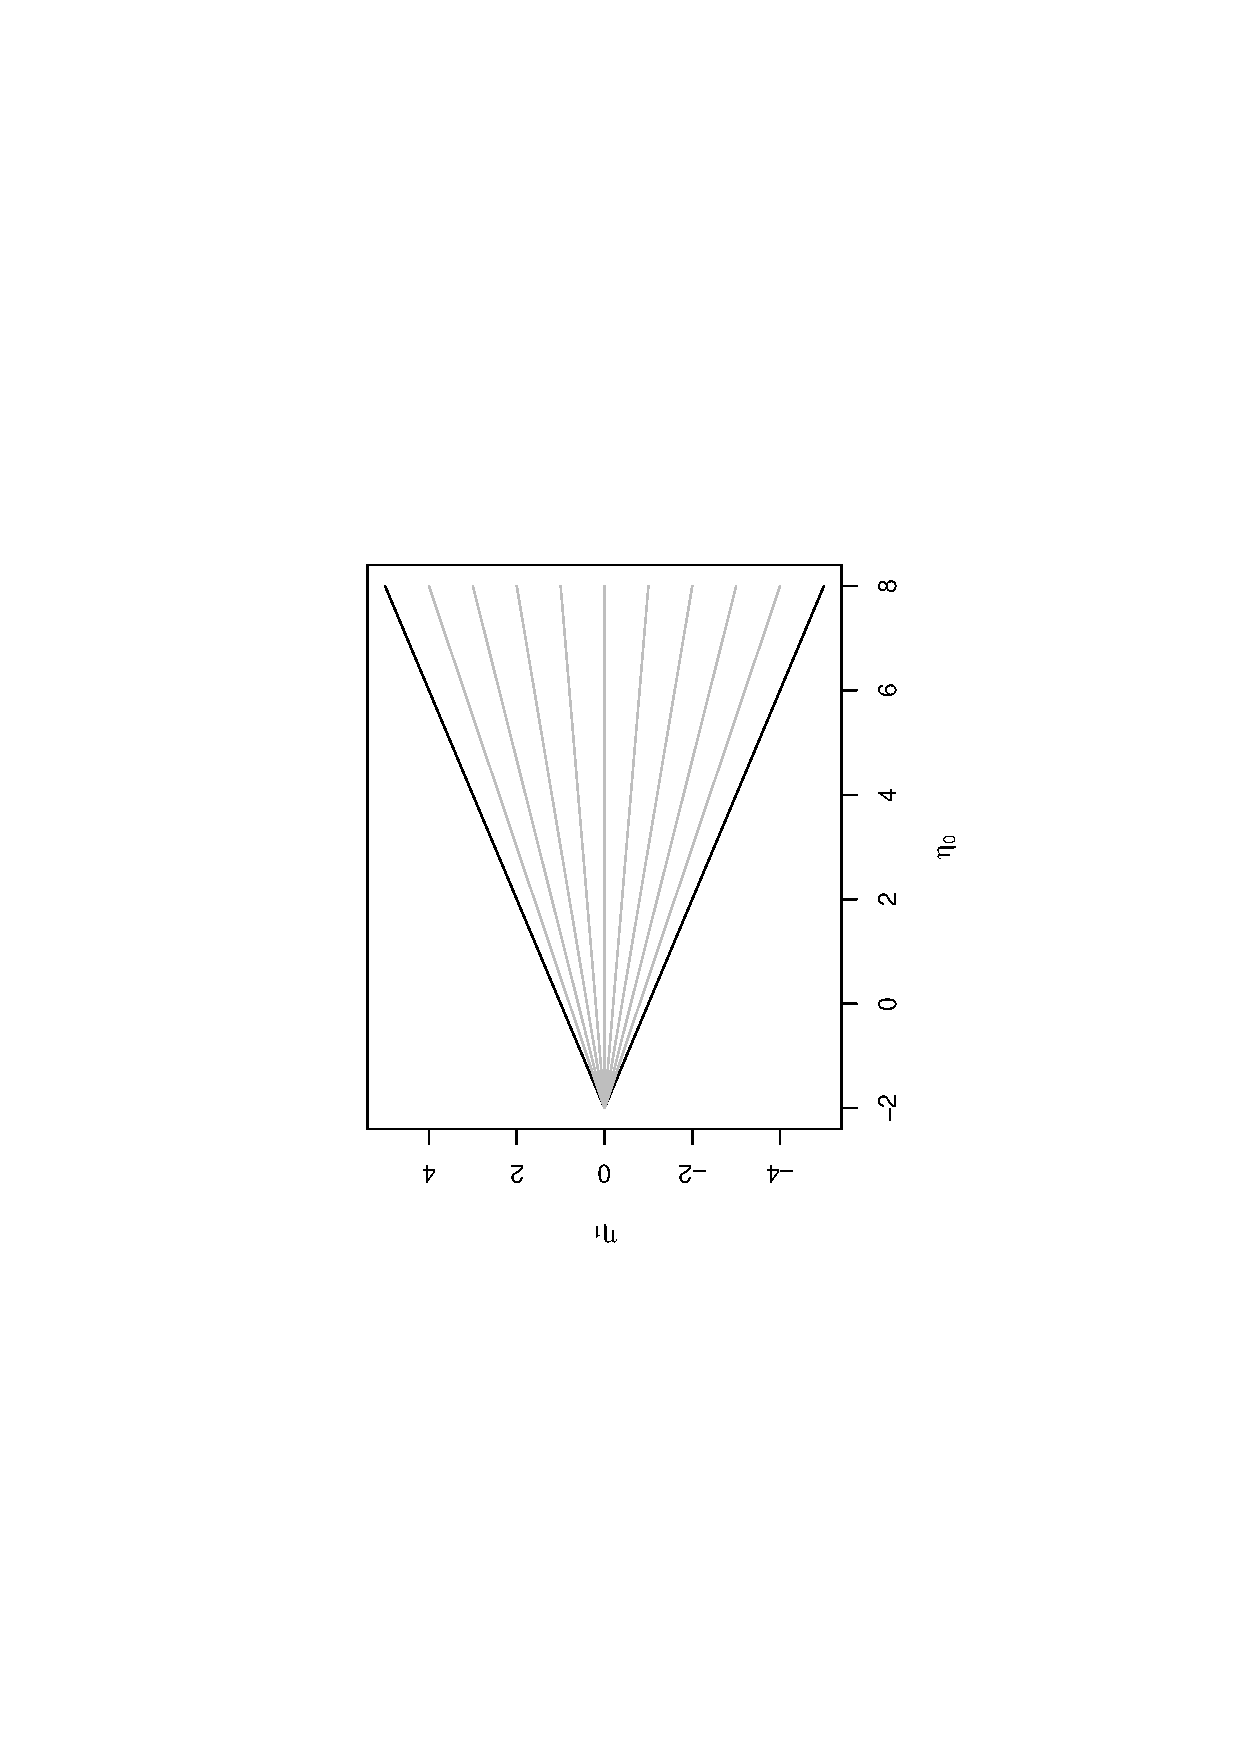
\includegraphics[trim = 80mm 45mm 80mm 60mm, clip, width=0.7\textwidth]{R/boatshape-domain}%
%}
\caption[Bounds for the domain of $\eta_0$ and $\eta_1$ for the Beta-Binomial model,
with rays of constant expectation for $y_c = \{0.1,0.2,\ldots,0.9\}$.]%
{Bounds for the domain of $\eta_0$ and $\eta_1$ for the Beta-Binomial model (black),
with rays of constant expectation for $y_c = \{0.1,0.2,\ldots,0.9\}$ (grey).}
\label{fig:boatshape-domain}
\end{figure}

As we wrote in Section~\ref{sec:concluding-outlook},
$\eta_1$ cannot have the convenient property of being equal to
the expectation of the mean sample statistic $\ttau(\x)$ (here, $s/n$),
as was the case for $y$.%
\footnote{For $\yz$, it holds that $\yz = \E\big[\E[\ttau(\x) \mid \psi] \mid \nz, \yz\big]$,
as mentioned in Section~\ref{sec:regularconjugates}.}
However, from \eqref{eq:trafotony} we can derive that coordinates $(\eta_0,\eta_1) \in \Eta$ satifying
\begin{align}
\label{eq:raysofconstantexpectation}
\eta_1 = f(\eta_0) &= (\eta_0 + 2)(y_c - \frac{1}{2}) 
\end{align}
will have a constant expectation $y_c$.
The domain $\Eta$, and these \emph{rays of constant expectation} emanating from the coordinate $(-2,0)$,
are depicted in Figure~\ref{fig:boatshape-domain}.


\subsection{Informal Rationale for Boat-Shaped Parameter Sets}
\label{boatshape-rationale}

When Mi\c{k}elis Bickis presented this parametrisation of conjugate priors at a talk,
both Frank Coolen and the author of this thesis had independently the same basic idea
for a set shape that allows for both \pdc\ sensitivity
%and gives `bonus precision' if prior and data agree especially well,
and more precise inferences in case of strong prior-data agreement.
The basic idea for this shape is described informally below,
while a suggestion for a parametrisation of such a shape is described and discussed
in Section~\ref{sec:boatshape-2}.

In the parametrisation in terms of $(\nz,\yz)$ and $(\nn, \yn)$,
posterior inferences become more precise,
because the stretch in the main parameter dimension $y$, denoted by $\Delta_y(\PN)$,
tends to $0$ for $n \to \infty$ (see the discussion in Section~\ref{sec:gbicp-properties-criteria}).
In the domain $\Eta$ as depicted in Figure~\ref{fig:boatshape-domain},
instead the rays of constant expectation fan out for growing $n$, %**move outwards to the right,
while a parameter set will retain its size in updating.
Increased precision in a posterior parameter set $\EN$, which is just
its prior counterpart $\EZ$ shifted to the right,
is given by the fact the more $\EN$ is located to the right,
the fewer rays of constant expectation $\EN$ will intercept.
Imprecision in terms of $\E\big[\E[\ttau(\x) \mid \psi] \mid \nn, \yn\big] = \yn$
can thus be imagined as the size of the `shadow' that a set $\EN$ casts
when considering a light source in $(-2,0)$ (the point from which the rays of constant expectation emanate).
In short, the smaller this shadow, the more precise the inferences.

In the context of the model from Section~\ref{sec:miksworld},
we will denote by $\ynl$ and $\ynu$ the bounds of this shadow,
i.e.,
\begin{align*}
\ynl &:= \min_{(\ezn,\eon) \in \EN} \yn = \min_{(\ezn,\eon) \in \EN} \frac{\eon}{\ezn+2} + \frac{1}{2}\,, \\
\ynu &:= \max_{(\ezn,\eon) \in \EN} \yn = \max_{(\ezn,\eon) \in \EN} \frac{\eon}{\ezn+2} + \frac{1}{2}\,,
\end{align*}
and we call the coordinates $\argmin_{(\eta_0,\eta_1) \in \EN} \yn$ and $\argmax_{(\eta_0,\eta_1) \in \EN} \yn$
the \emph{touchpoints} of $\EN$ responsible for the shadow $[\ynl, \ynu]$.
Mutatis mutandis, the same definitions can be made for the prior set $\EZ$.

Due to the fanning out of rays, most shapes for $\EZ$ will lead to decreasing imprecision for increasing $n$.
Indeed, models of type~(\ref{enum:modeltypes-a}) from Section~\ref{sec:basicsetting},
where $\PZ = \nz \times [\yzl, \yzu]$,
are represented here again by a line segment $\EZ = \ezz \times [\eozl,\eozu]$,
such that the posterior touchpoints are, for any $s$ and $n$, $(\ezn,\eonl)$ and $(\ezz,\eonu)$,
where $\eonl$ and $\eonu$ are the updated versions of $\eozl$ and $\eozu$, respectively.
Due to \eqref{eq:eta-update}, it holds that $\eonu-\eonl = \eozu-\eozl$;
therefore, imprecision decreases here because a line segment of fixed size
will cast a smaller shadow when further to the right,
as illustrated in Figure~\ref{fig:boatshape-vertical}.

\begin{figure}  %trim=l b r t
\centering
%\fbox{%
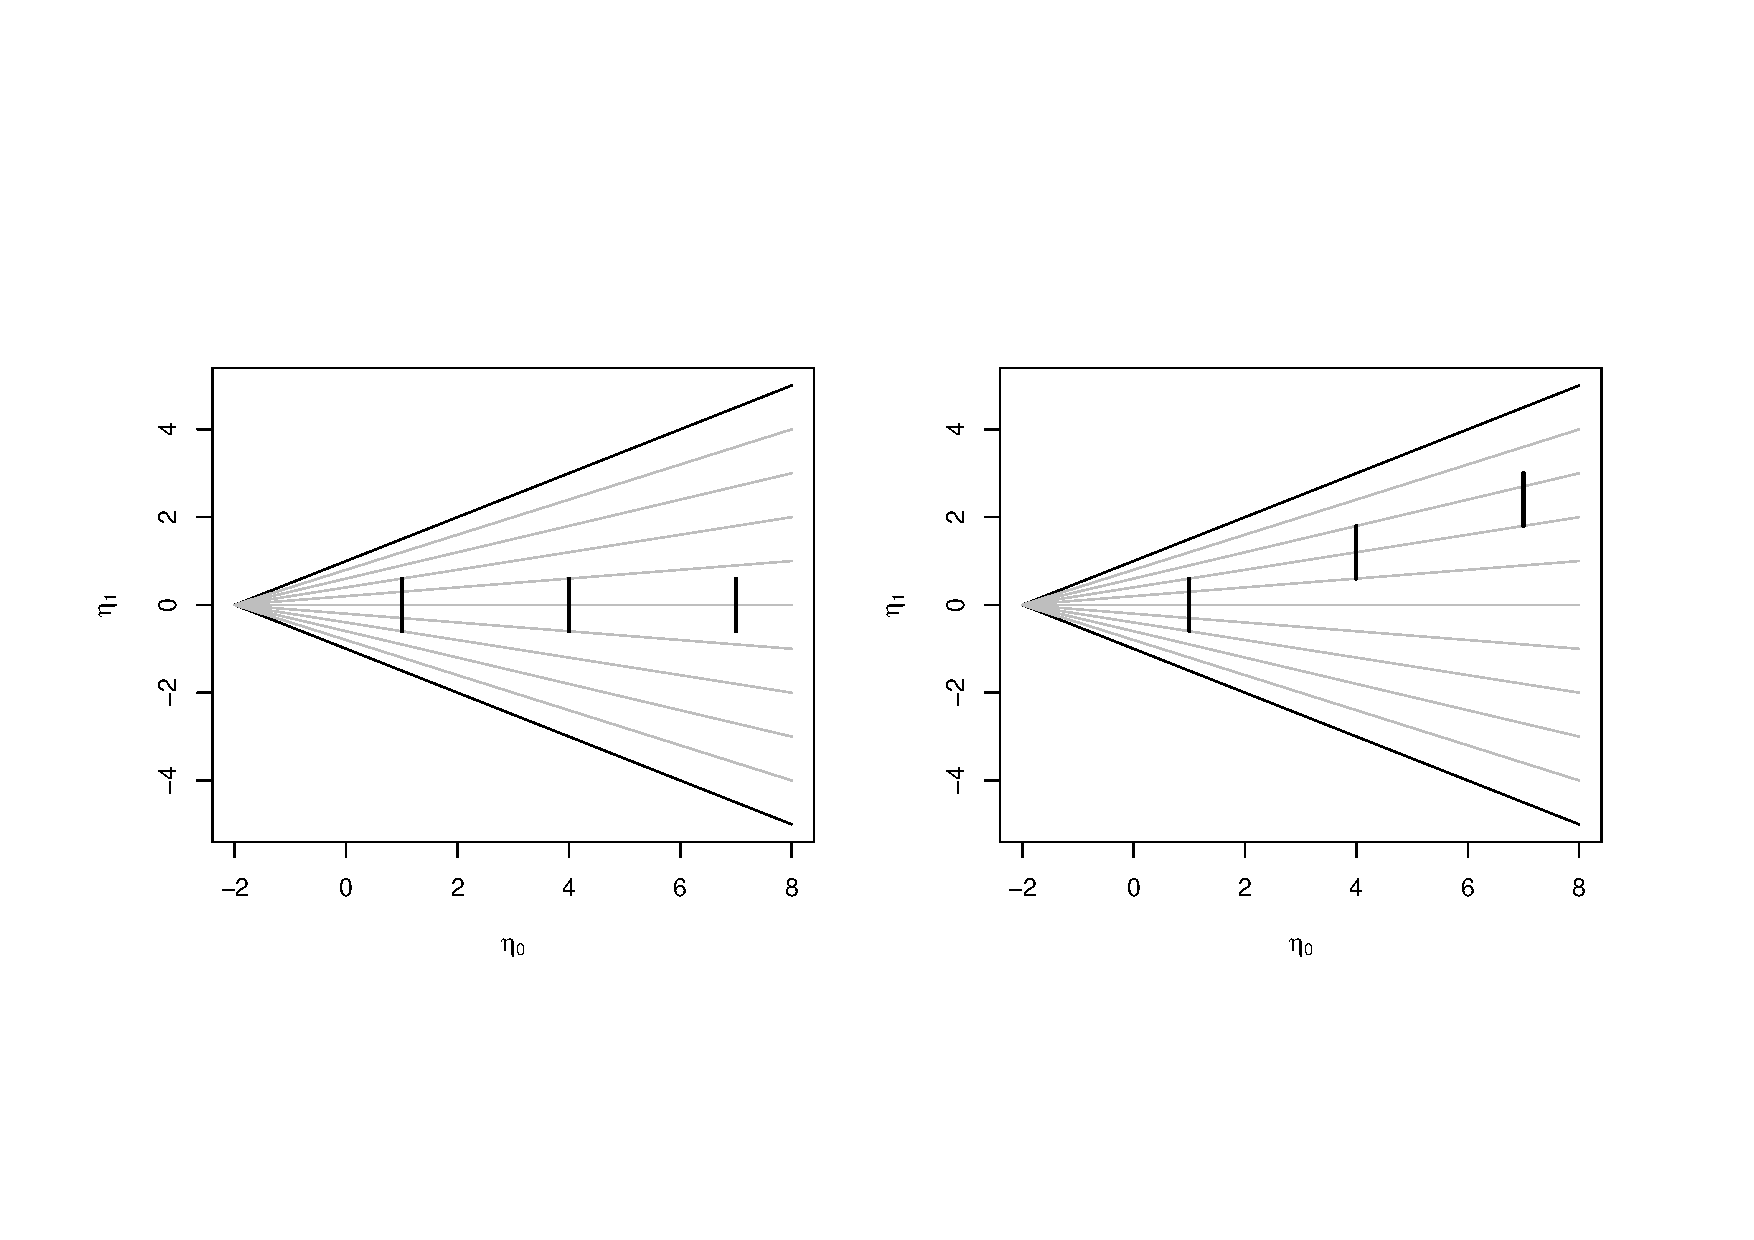
\includegraphics[trim = 15mm 45mm 25mm 60mm, clip, width=\textwidth]{R/boatshape-vertical}%
%}
\caption[Line segment parameter set $\EZ$ %
and respective posterior sets for $s/n=0.5$ and $s/n=0.9$.]%
{Parameter set $\EZ = \ezz \times [\text{\underline{$\eta$}${}_1\uz$},\eozu]$ and respective posterior sets $\EN$
for $s/n=0.5$ (left) and $s/n=0.9$ (right). Note that all sets have the same size,
imprecision decreasing only through their position on the $\eta_0$ axis.}
\label{fig:boatshape-vertical}
\end{figure}

For \pdc\ sensitivity, we need shapes that cover a range of $\eta_0$ values,
for the same reasons as in the framework of Section~\ref{sec:basicsetting},
where only sets with a range of $\nz$ values offered this property.
Sets that are elongated along the rays of constant expectation
will behave here similar to the rectangular shapes of Section~\ref{sec:basicsetting}.
When shifted along its respective ray of constant expectation,
imprecision will be reduced as the shadow of the set will become smaller just as described above for line segments.
When such a shape is instead shifted away from its ray of constant expectation,
imprecision will be increased, as a prolonged shape that is now turned away from its ray 
will cast a larger shadow.%
\footnote{This will become clear from the depiction of boatshape sets in Figure~\ref{fig:boatshape-posterior-mik}.} 

A set $\EZ$ allowing for less imprecison in case of strong prior-data agreement
must also be able to cast a smaller shadow if the update shift goes into the direction of its ray,
%of $s/n$ according the information,
but we will enhance this effect by considering now also the properties
of the canonical posteriors the coordinates of $\EN$ represent.

We have seen that for the conjugate distributions themselves,
$\nz$ is generally a parameter determining the spread of the distribution
(e.g., in the Normal-Normal model (see Section~\ref{sec:norm-norm}), $\nz$ was the inverse variance),
such that we will have more precise inferences if the shadow bounds $\ynl$ and $\ynu$
are attained at higher values of $\eta_0$, leading to lower variances in the
`critical' distributions at the boundary of the posterior expectation interval $[\ynl,\ynu]$.
For this to happen, we need a shape for which the touchpoints responsible for $\ynl$ and $\ynu$
are attained at higher values of $\eta_0$ in case of strong prior-data agreement.
Shapes that accomplish this must have a curvature along their length in the direction
of the constant rays of expectation.
The shape we suggest thus looks like a bullett, or like a boat with a transom stern
(see, e.g., Figure~\ref{fig:boatshape-prior}).



\subsection{The Boatshape}
\label{sec:boatshape-2}

In this Section, %~\ref{sec:boatshape-2} below,
%Now,
we will suggest a parametrisation for such a shape.
The definition, along with some first graphical examples, is given in Section~\ref{sec:basicdefboat},
and we discuss some first technical results for this shape in Sections~\ref{sec:touchpoints} -- \ref{sec:generalupdate}.

\subsubsection{Basic Definition}
\label{sec:basicdefboat}

We will now present a parametrisation for such a boat-shaped parameter set $\EZ$.
To keep things simple, we will consider here and in the follwing only prior sets
that are symmetric around the $\eta_0$ axis, i.e., centered around $y_c = 0.5$,
expressing prior the information that we deem a fraction of successes of $\frac{s}{n} = \frac{1}{2}$
as the most probable.%
\footnote{The general case of sets $\EZ$ with central ray $y_c \neq 0.5$
is discussed informally in Section~\ref{sec:boatshape-outlook}.}

For the contours of $\EZ$, we suggest an exponential function as the functional form,
where the `prow' of the set is located at $(\ezl, 0)$.
The lower and the upper contour $\czl(\eta_0)$ and $\czu(\eta_0)$ are defined as
\begin{align*}
\czl(\eta_0) &= -a \left( 1 - e^{-b(\eta_0 - \ezl)} \right)\,, \\
\czu(\eta_0) &= \phantom{-}%
                 a \left( 1 - e^{-b(\eta_0 - \ezl)} \right)\,, 
\end{align*}
where $a$ and $b$ are parameters controlling the shape.
We will also need the respective derivations with respect to $\eta_0$, given by
\begin{align*}
\frac{d}{d\eta_0} \czl(\eta_0) &= -ab e^{-b(\eta_0 - \ezl)}\,, \\
\frac{d}{d\eta_0} \czu(\eta_0) &= \phantom{-}%
                                   ab e^{-b(\eta_0 - \ezl)}\,.
\end{align*}

For this basic situation, given the parameters $\ezl$, $\ezu$, $a$, and $b$,
$\EZ$ is thus defined as
\begin{align}
\label{eq:basicset}
\EZ =
\{(\eta_0,\eta_1) \colon \ezl \le \eta_0 \le \ezu, \czl(\eta_0) \le  \eta_1 \le \czu(\eta_0) \}\,.
\end{align}
A prior boatshape set with $\ezl=1$, $\ezu=6$, $a=2$, and $b=0.8$ is depicted in Figure~\ref{fig:boatshape-prior},
where the left graph shows this set as defined in terms of $(\eta_0,\eta_1)$,
and the right graph shows the set from the left transformed into the space $\N \times \Y$.

\begin{figure}  %trim=l b r t
\centering
%\fbox{%
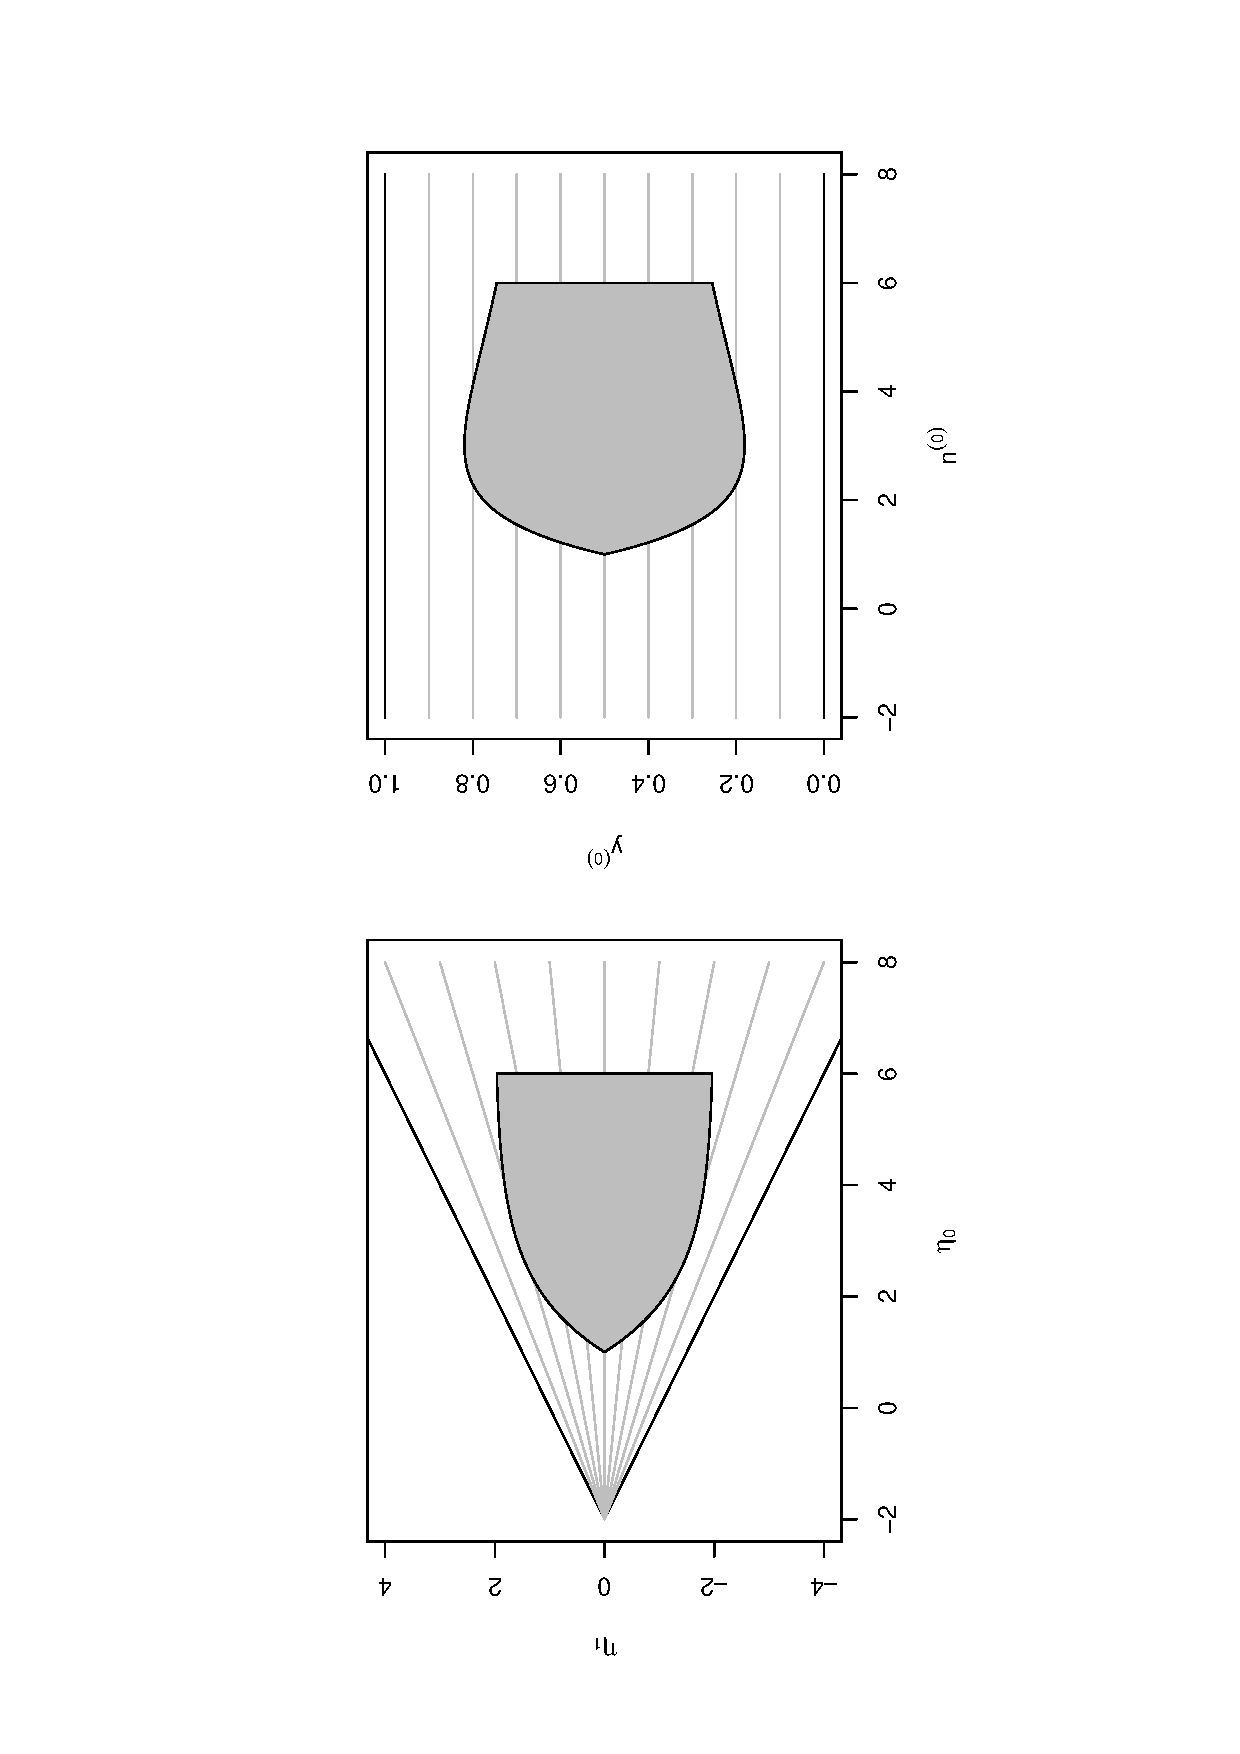
\includegraphics[trim = 15mm 45mm 25mm 60mm, clip, width=\textwidth]{R/boatshape-prior}%
%}
\caption[Boatshape prior set in the parametrisation via $(\eta_0,\eta_1)$ and via $(\nz,\yz)$.]%
{Boatshape prior set in the parametrisation via $(\eta_0,\eta_1)$ (left) and via $(\nz,\yz)$ (right),
with parameters $\ezl=1$, $\ezu=6$, $a=2$, and $b=0.8$.}
\label{fig:boatshape-prior}
\end{figure}


We have as yet no good formal description for the role of the parameters $a$ and $b$. %that,
%togeher with $\ezl$ and $\ezu$, define the boat-set (see Section~\ref{sec:basicdefboat} below).
Informally, $a$ determines the half-width of the set;
the width, i.e., the size in the $\eta_1$ dimension, would be $a$ if $\ezu \to \infty$.
$b$ instead determines the `bulkyness' of the shape.
Together with $\ezl$, $a$ and $b$ determine the prior interval for the expected success probability $[\yzl, \yzu]$.
For fixed $\ezl$ and $a$, increasing $b$ leads to a wider prior expectation interval.
For $[\yzl, \yzu]$, the choice of $\ezu$ is irrelevant.%
\footnote{$\ezu$ plays only a role in determining when the `unhappy learning' phase starts
(see end of Section~\ref{sec:generalupdate}).}


\begin{figure}  %trim=l b r t
\centering
%\fbox{%
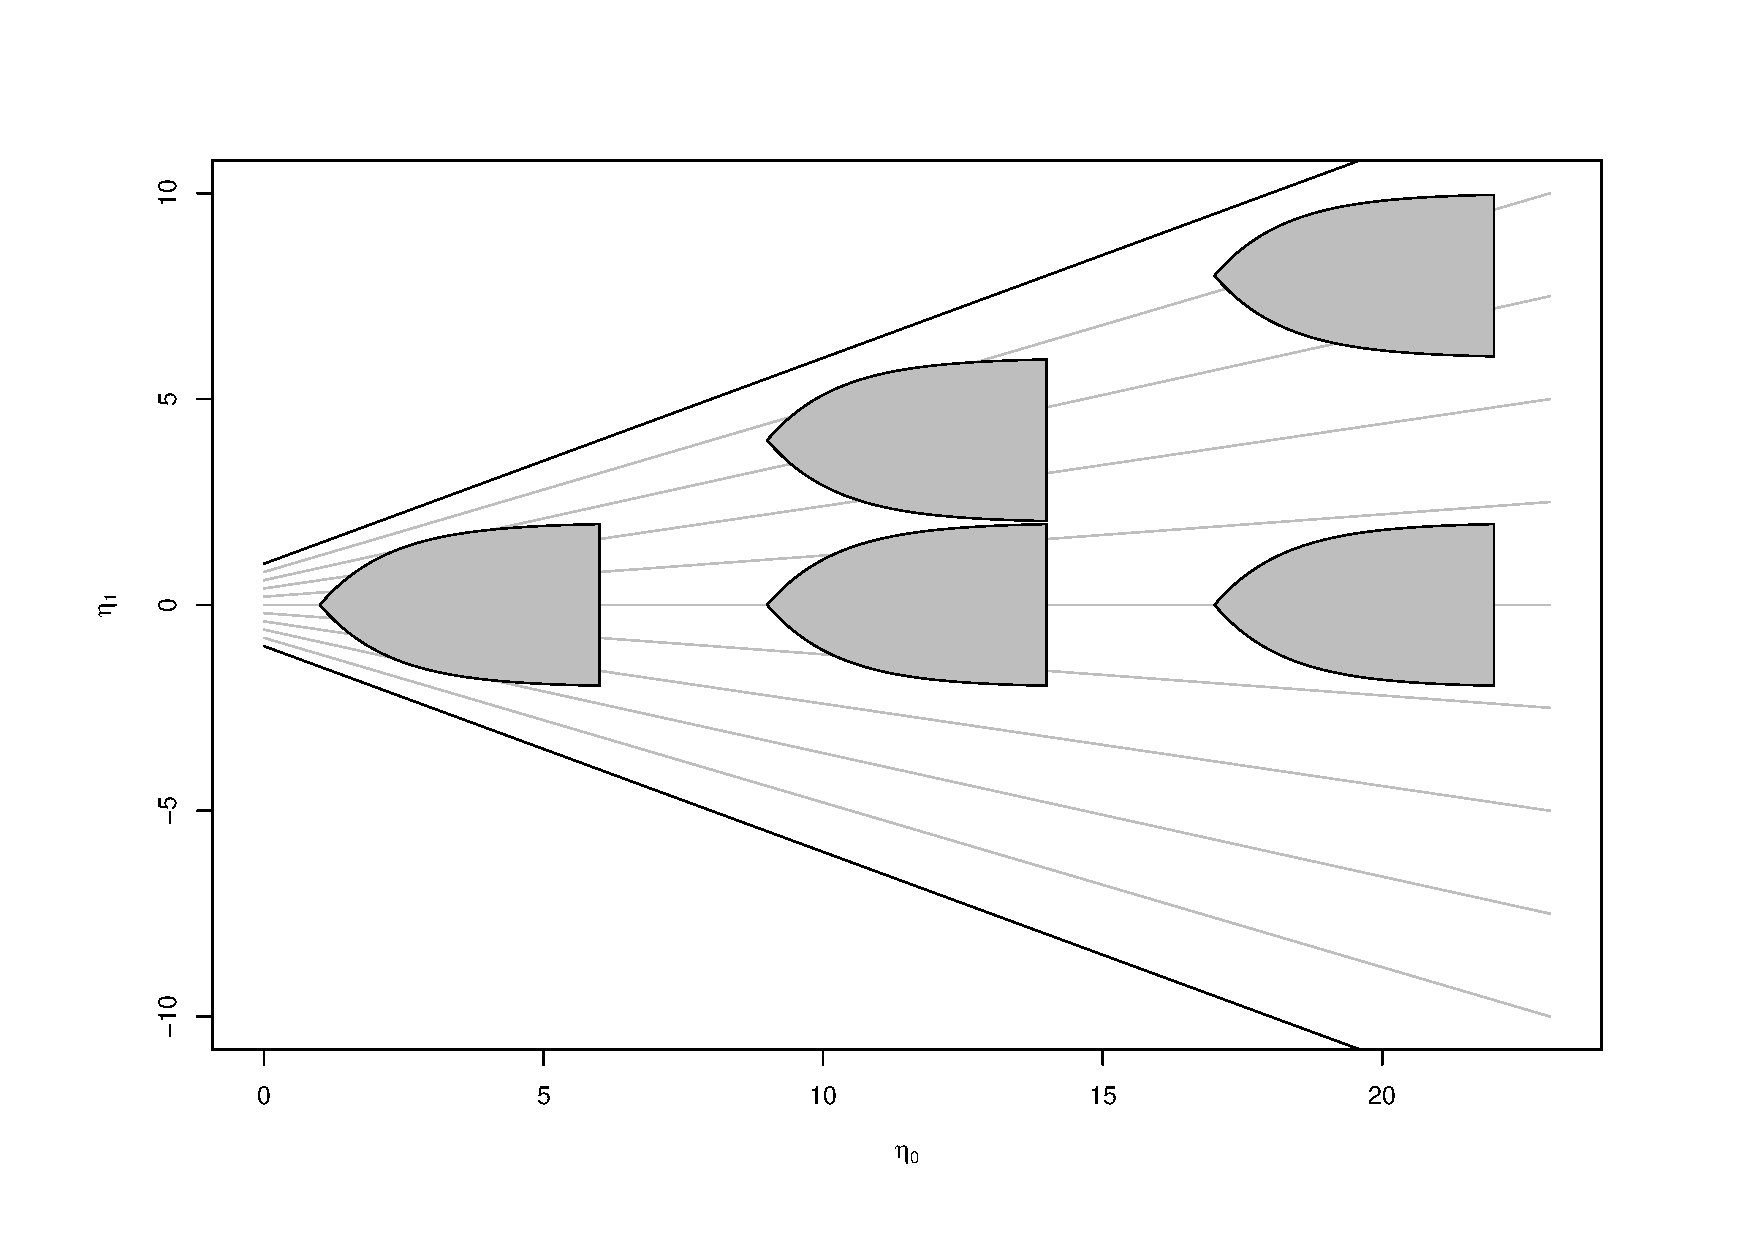
\includegraphics[trim = 20mm 35mm 30mm 45mm, clip, width=\textwidth]{R/boatshape-posterior-mik}%
%}
\caption[Boatshape prior and posterior sets for data in accordance and in conflict with the prior.]%
{Boatshape prior and posterior sets for data in accordance and in conflict with the prior.
The prior set is the same as in Figure~\ref{fig:boatshape-prior}.
While the posterior sets for $\frac{s}{n}=0.5$ move along the ray for $y_c=0.5$,
the posterior sets for $\frac{s}{n}=1$ are shifted away from the ray for $y_c=0.5$,
resulting in increased posterior imprecision.
Note that lower and upper touchpoints are in the middle of the contour
for the prior and the posterior resulting for data $\frac{s}{n}=\frac{4}{8}$,
while at least one touchpoint is at the end for all other sets.
(see also Figure~\ref{fig:boatshape-posterior-normal}).}
\label{fig:boatshape-posterior-mik}
\end{figure}


\begin{figure}  %trim=l b r t
\centering
%\fbox{%
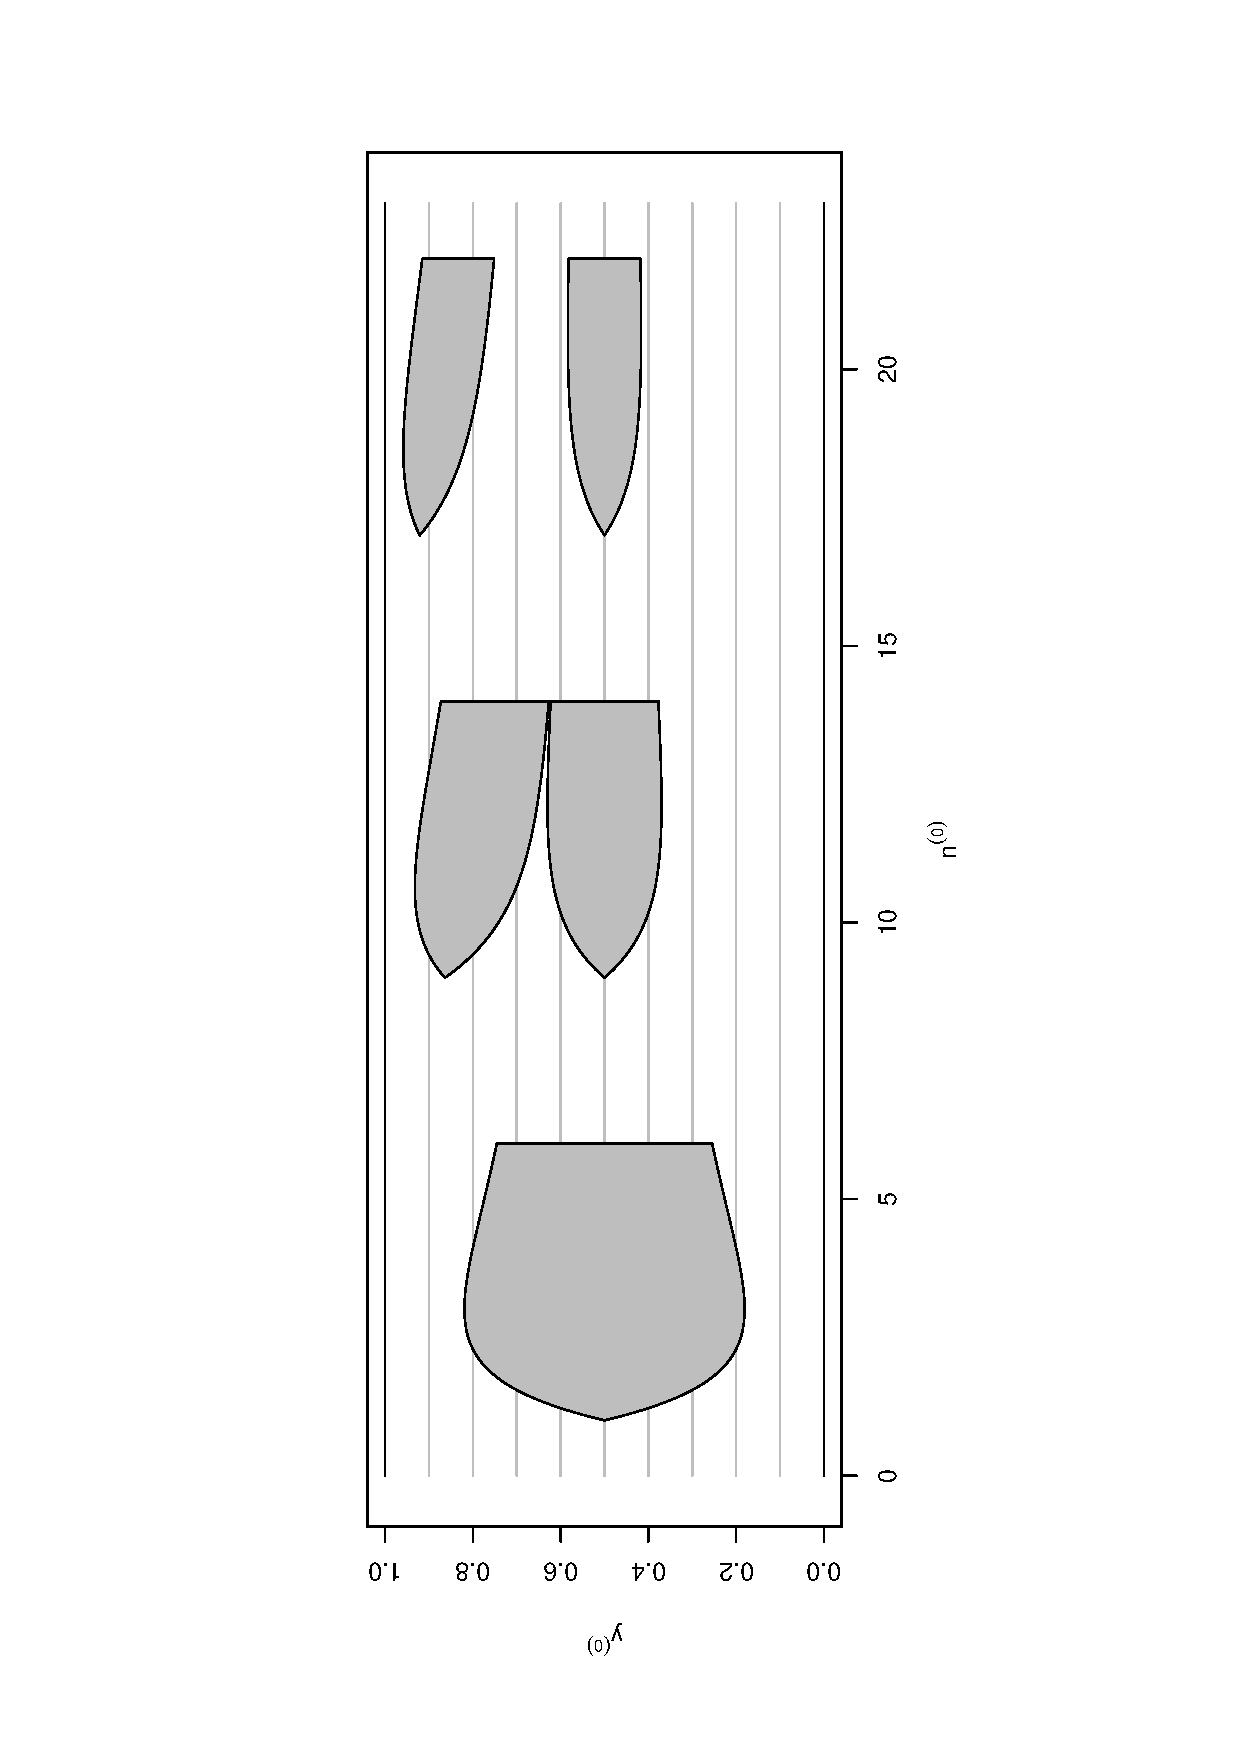
\includegraphics[trim = 15mm 45mm 25mm 60mm, clip, width=\textwidth]{R/boatshape-posterior-normal}%
%}
\caption[Boatshape prior and posterior sets from Figure~\ref{fig:boatshape-posterior-mik} in the parametrisation via $(\nz,\yz)$.]%
{Boatshape prior and posterior sets from Figure~\ref{fig:boatshape-posterior-mik} in the parametrisation via $(\nz,\yz)$.
Note that in the strong prior-data agreement case,
posteriors based on a rectangular set with the same prior main parameter imprecision
would be larger than the ones depicted here, illustrating the extra gain in precision.}
\label{fig:boatshape-posterior-normal}
\end{figure}


\subsubsection{Finding the Touchpoints for the Basic Set}
\label{sec:touchpoints}

In contrast to models discussed in Section~\ref{sec:generalmodel},
where $\yzl$ and $\yzu$ were at either ends of a set $\PZ$,
here, for a set \eqref{eq:basicset}, the touchpoints $\yzl$ and $\yzu$ 
are not necessarily at $\ezzl$ or $\ezzu$.
\footnote{See, e.g., the prior in Figure~\ref{fig:boatshape-prior}.}
Instead, the rays of constant expectation \eqref{eq:raysofconstantexpectation}
touching the parameter set must be determined to find $\yzl$ and $\yzu$.
To do this, the tangent equations for the lower and the upper contour function
depending on $\eta_0$ are determined.
As all rays of constant expectation pass through the point $(-2,0)$,
the tangent that passes through this point is determined by inserting this point
into the tangent equation, and the resulting equation is solved for $\eta_0$.
The resulting points $(\eta_0^u,\czu(\eta_0^u))$ resp.\ $(\eta_0^l,\czl(\eta_0^l))$
then give the touchpoints of the parameter set,
and can be transformed to $\yzl$ and $\yzu$ by using \eqref{eq:trafotony}.

As the basic set is symmetrical to the $\eta_0$ axis, $\eta_0^u = \eta_0^l$,
and it suffices to find, e.g., $\eta_0^u$, by considering the upper contour tangent.

We denote the tangent in contour point $(\eta_0,\czu(\eta_0))$ by
\begin{align*}
\ol{t}_{\eta_0}(x) &= dx + i\,,
\end{align*}
where $d = \frac{d}{d\eta_0} \czu(\eta_0)$ and
$i$ such that $\ol{t}_{\eta_0}(x)$ goes through the point $(\eta_0,\czu(\eta_0))$:
\begin{align*}
\ol{t}_{\eta_0}(x) &= dx + i \quad \equiv\\
\czu(\eta_0) &= \frac{d}{d\eta_0} \czu(\eta_0) \eta_0 + i \\
i &= \czu(\eta_0) -\frac{d}{d\eta_0} \czu(\eta_0) \eta_0 \\
  &= a - a e^{-b(\eta_0 - \ezl)} - \eta_0 ab e^{-b(\eta_0 - \ezl)} \\
  &= a - a (1 + b \eta_0) e^{-b(\eta_0 - \ezl)} \\
\Longrightarrow\quad
\ol{t}_{\eta_0}(x) &= ab e^{-b(\eta_0 - \ezl)} x + a - a (1 + b \eta_0) e^{-b(\eta_0 - \ezl)} \\
                   &= a - a \big(1 + b(\eta_0-x)\big) e^{-b(\eta_0 - \ezl)}
\end{align*}

Now, let us find the touchpoint $(\eta_0^u, \czu(\eta_0^u))$ whose tangent goes through $(-2,0)$, as this gives us $\yzu$.
We insert $(-2,0)$ into the tangent equation and solve for $\eta_0$.
\begin{align}
a - a \big(1 + b(\eta_0^u + 2)\big) e^{-b(\eta_0^u - \ezl)} &\stackrel{!}{=} 0 \nonumber\\
1 + b(\eta_0^u + 2) &\stackrel{!}{=} e^{b(\eta_0^u - \ezl)} \label{eq:eta0u}
\end{align}
This equation has only one solution for $\eta_0^u > \ezl$, that is,
however, not available in closed form.

As a general rule, the nearer $\eta_0^u$ is to $\ezl$, the larger $\frac{d}{d\eta_0} \czu(\eta_0^u)$,
that is, $\yzu$ %the upper expected value for the prior set
is more away from $\frac{1}{2}$.
Here, this means that the larger $\eta_0^u$, the more imprecise is the prior parameter set.


\subsubsection{Strong Prior-Data Agreement Property}
\label{sec:spda-property}

We will now prove the essential property that sets \eqref{eq:basicset}
will lead to especially precise inferences when data are strongly suporting prior information.

For a prior parameter set $\EZ = \ezz \times [\eozl,\eozu]$
%, with $\eta_0 = \ezz$ fixed and $\eta_1$ varying in an interval $[\eol, \eou]$
symmetric around $0$,
the prior upper expected value $\yzu$
results from the transformation \eqref{eq:trafotony} of the point $(\ezz,\eozu)$.
The posterior upper expected value $\ynu$,
given data that coincide especially well with the prior,
i.e., data with $s = \frac{n}{2}$, will then be found at the point $(\ezz+n,\eozu)$,
because in this case, the set does not move in the vertical ($\eta_1$) direction.
As $\yz$ is decreasing in $\eta_0$ and $\eta_1$ is constant, $\ynu$ %the posterior upper expected value
will be lower than $\yzu$, i.e., imprecision is reduced.

Imprecision is, however, even more strongly reduced for the boatshape parameter set \eqref{eq:basicset}.
Say, we define the prior parameter set such that the prior upper touchpoint
is at the $\eta_0$ coordinate $\eta_0^u = \ezz$.
For this shape, the $\eta_0$ coordinate for the posterior upper touchpoint ${\eta_0^u}\un$
will be  larger than the updated $\ezz$, i.e., ${\eta_0^u}\un > \ezz + n$ (as will be shown below), and thus $\ynu$ is lower.
Although the $\eta_1$ coordinate will be slightly larger at the point $({\eta_0^u}\un, \ol{c}({\eta_0^u}\un))$
as compared to the point $(\ezz+n,\eozu)$, the corresponding $\ynu$ is still lower,
as it holds that
\begin{align*}
\frac{d}{d\eta_0} \ol{c}({\eta_0^u}\un) < \frac{d}{d\eta_0} \ol{c}(\ezz + n)
\end{align*}
because $\frac{d}{d\eta_0} \ol{c}(\eta_0)$ is decreasing in $\eta_0$,
and a smaller slope for the tangent through $(-2,0)$ is equivalent to a lower $\ynu$.
This is the desired reduction in imprecision for the case of strong prior-data agreement,
also depicted exemplarily in Figures~\ref{fig:boatshape-posterior-mik} and \ref{fig:boatshape-posterior-normal}.

The property ${\eta_0^u}\un > \ezz + n$ of the boatshape set will be shown below.
Due to symmetry of prior and posterior parameter shape around the $\eta_0$ axis,
${\eta_0^u}\un = {\eta_0^l}\un$, i.e.,
the touchpoint at the upper contour (giving $\ynu$) is equal to
the touchpoint at the lower contour (giving $\ynl$),
and thus, the argument formulated in terms of ${\eta_0^u}\un$ holds also for ${\eta_0^l}\un$.

The upper exponential contour for the posterior boatshape,
updated with $s = \frac{n}{2}$, has its `prow' now at $(\ezl + n, 0)$,
and is defined by the function
\begin{align*}
\ol{c}(\eta_0) &= a \left( 1 - e^{-b(\eta_0 - n -\ezl)} \right) \\
\frac{d}{d\eta_0} \ol{c}(\eta_0) &= ab e^{-b(\eta_0 - n - \ezl)} \,.
\end{align*}

The tangent in contour point $(\eta_0,\ol{c}(\eta_0))$ is
\begin{align*}
\ol{t}_{\eta_0}(x) &= a - a \big(1 + b(\eta_0-x)\big) e^{-b(\eta_0 - n - \ezl)} \,.
\end{align*}

Again, we insert $(-2,0)$ into this tangent equation and solve for $\eta_0$.
\begin{align}
a - a \big(1 + b({\eta_0^u}\un + 2)\big) e^{-b({\eta_0^u}\un - n - \ezl)} &\stackrel{!}{=} 0 \nonumber\\
1 + b({\eta_0^u}\un + 2) &\stackrel{!}{=} e^{b({\eta_0^u}\un - n - \ezl)} \,.\label{eq:eta0uposterior}
\end{align}
We compare now \eqref{eq:eta0uposterior} to \eqref{eq:eta0u} and conclude
that indeed ${\eta_0^u}\un > \ezz + n$.

\begin{figure}
\centering
\begin{tikzpicture}[pin distance=1cm]
\node (0,0) {%\fbox{% %trim=l b r t
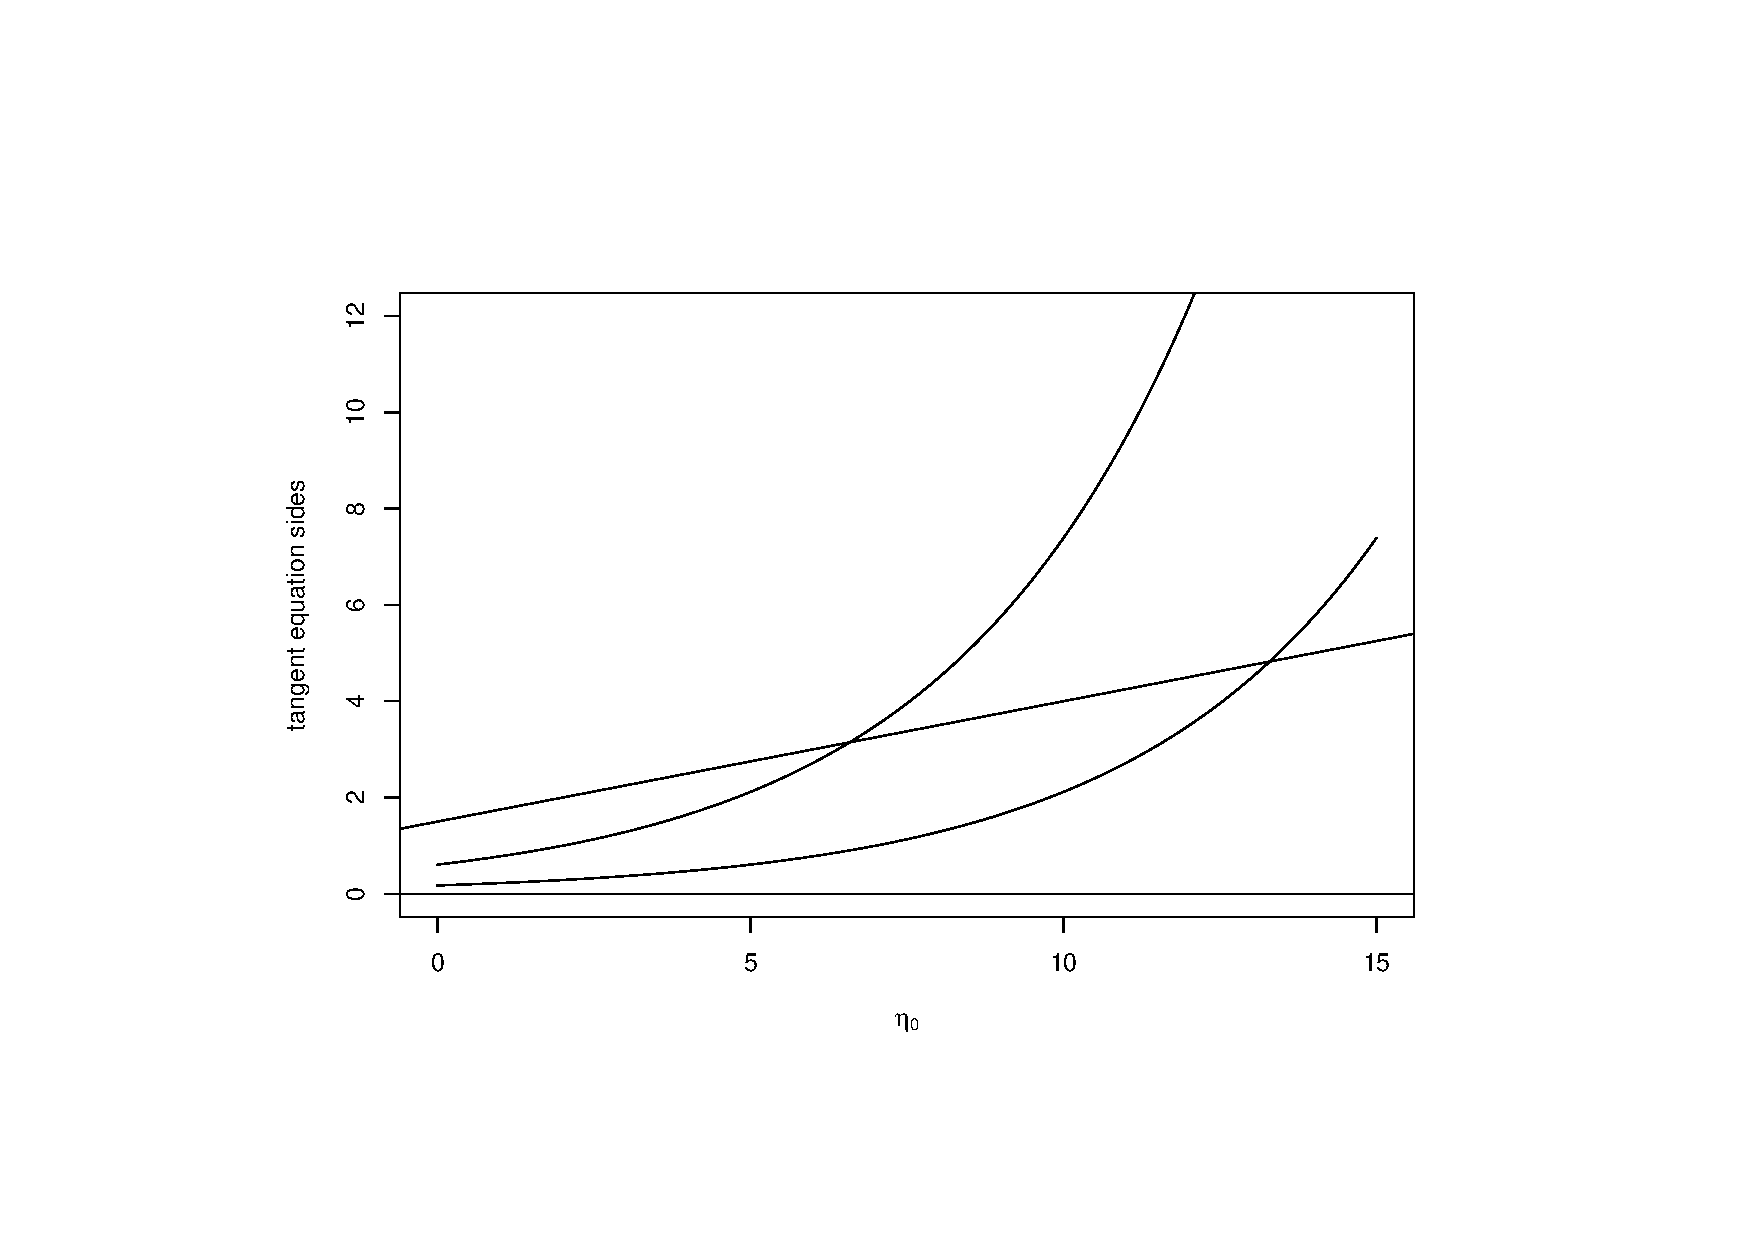
\includegraphics[trim = 45mm 35mm 45mm 45mm, clip, width=\textwidth]{R/prior-vs-posterior-eta0u}%
};
\coordinate (x1) at (-0.35,-1.21);
\draw (x1) circle (2.5pt);
\coordinate [pin=-93:${\eta_0^u}\uz$] (a1) at (-0.35,-3.24);
\draw[dashed] (x1) -- (a1);
\coordinate (x2) at ( 5.2 ,-0.15);
\draw (x2) circle (2.5pt);
\coordinate [pin=-75:${\eta_0^u}\un$] (a2) at ( 5.2,-3.24);
\draw[dashed] (x2) -- (a2);
\coordinate (x1n) at (3.8,-1.21);
%\draw (x1n) circle (2.5pt);
%\coordinate [label=below:${\eta_0^u}\uz + n$] (a1n) at (3.8,-3.5);
\coordinate [pin=-93:${\eta_0^u}\uz + n$] (a1n) at (3.8,-3.24);
\draw[dashed] (x1) -- (x1n) -- (a1n);
\end{tikzpicture}
\caption{Illustration for the argument that ${\eta_0^u}\un > {\eta_0^u}\uz + n$.}
\label{fig:spda1}
\end{figure}

In Figure~\ref{fig:spda1}, the two exponential graphs have the same curvature,
the right one is the same as the left, only being shifted to the right by $n$.
The value of $\ezz + n$, defined as the abscissa of the intersection of the left exponential and the linear function,
being shifted to the right by $n$, would thus be on the right exponential curve.
Because ${\eta_0^u}\un$ results from the intersection of the right exponential curve and the linear function,
it is necessarily larger than ${\eta_0^u}\uz + n$, as the linear function is increasing.


\subsubsection{General Update with \texorpdfstring{$s > \frac{n}{2}$}{s > n/2}}
\label{sec:generalupdate}

Let us now consider the update of the basic boatshape \eqref{eq:basicset} %symmetric around the $\eta_0$ axis,
in the general case $s \neq \frac{n}{2}$.
Due to symmetry of the prior set, we can, without loss of generality,
consider again only the case $s > \frac{n}{2}$.

For the prior set, being symmetric around the $\eta_0$ axis,
both touchpoints are located at the same $\eta_0$ coordinate,
the resulting $\yzl$ and $\yzu$ having the same distance to $0.5$.
Regarding the posterior set, according to \eqref{eq:eta-update},
$\eta_0$ coordinates are incremented by $n$, while
$\eta_1$ coordinates are incremented by $s+\frac{n}{2}$.
That is, if $s \neq \frac{n}{2}$, the updated set is no longer symmetric around the $\eta_0$ axis,
such that we must consider the lower and upper contours separately.

The upper and lower contours and their respective derivatives for the updated boatshape set are now
\begin{align*}
\ol{c}(\eta_0)                   &= s - \frac{n}{2} + a - a e^{-b(\eta_0 - n - \ezl)} \,,\\
\frac{d}{d\eta_0} \ol{c}(\eta_0) &=                      ab e^{-b(\eta_0 - n - \ezl)} \,,\\
\ul{c}(\eta_0)                   &= s - \frac{n}{2} - a + a e^{-b(\eta_0 - n - \ezl)} \,,\\
\frac{d}{d\eta_0} \ul{c}(\eta_0) &=                     -ab e^{-b(\eta_0 - n - \ezl)} \,.
\end{align*}
The upper and lower tangents in contour point $(\eta_0,c(\eta_0))$ are now given by
\begin{align*}
\ol{t}_{\eta_0}(x) &= s - \frac{n}{2} + a - a \big(1 + b(\eta_0-x)\big) e^{-b(\eta_0 - n - \ezl)} \,,\\
\ul{t}_{\eta_0}(x) &= s - \frac{n}{2} - a + a \big(1 + b(\eta_0-x)\big) e^{-b(\eta_0 - n - \ezl)} \,.
\end{align*}
Inserting again $(-2,0)$, we get the equations defining the $\eta_0$ coordinates
${\eta_0^u}\un$ and ${\eta_0^l}\un$
that give us $\ynu$ and $\ynl$, respectively:
\begin{align}
%s - \frac{n}{2} + a - a \big(1 + b(\eta_0^u + 2)\big) e^{-b(\eta_0^u - n - \ezl)} &\stackrel{!}{=} 0 \nonumber\\
\label{eq:eta0u-general}
\frac{a}{s - \frac{n}{2} + a} \big(1 + b(\eta_0^u + 2)\big) &\stackrel{!}{=} e^{b(\eta_0^u - n - \ezl)} \,,\\
\label{eq:eta0l-general}
\frac{a}{\frac{n}{2} -s  + a} \big(1 + b(\eta_0^u + 2)\big) &\stackrel{!}{=} e^{b(\eta_0^u - n - \ezl)} \,.
\end{align}

We see thus that the picture from Figure~\ref{fig:spda1} holds here as well,
except that the linear function (left hand side of equations
\eqref{eq:eta0u-general} and \eqref{eq:eta0l-general}) is changed in slope and intercept by a factor.
(Equivalently, we can consider it to be rotated around the root $-2-\frac{1}{b}$.)
For $s=\frac{n}{2}$, this factor is 1 for both the lower and the upper touchpoint,
resulting in the situation of strong prior-data agreement as considered in Section~\ref{sec:spda-property},
where ${\eta_0^u}\un = {\eta_0^l}\un$ moved to the right.

Due to symmetry, we will consider the case $s > \frac{n}{2}$ only 
to describe ${\eta_0^u}\un$ and ${\eta_0^l}\un$.

\paragraph{Description of ${\eta_0^u}\un$.}

The factor to the linear function $\frac{a}{s - \frac{n}{2} + a}$
in \eqref{eq:eta0u-general} is smaller than $1$ and decreasing in $s$.
Thus, the larger $s$, the smaller the factor, the most extreme case being $s=n$,
where the factor is $\frac{a}{\frac{n}{2} + a}$.
As the linear function's slope will be less steep (the intercept is lowered as well),
%\footnote{The common root of the linear functions for any $s$ is at $\eta_0 = -2 -\frac{1}{b}$.}
the intersection with the exponential function moves to the left,
i.e.\ $\eta_0^u(s) < \eta_0^u(\frac{n}{2})$ for $\frac{n}{2} < s \le n$.
This means that $\ynu(s) > \ynu(\frac{n}{2})$ in general.
However, decrease of $\eta_0^u(s)$ is limited by $\ezl+n$.
When the intersection point reaches the left end of the shape at $\ezl+n$,
the gradual increase of $\ynu$ through the changing tangent slope 
for $\ezl+n \le \eta_0^u(s) \le \eta_0^u(\frac{n}{2})$ is replaced
by a different change mechanism,
where increase of $\ynu$ is solely due to increase in the $\eta_1$ direction.
Due to \eqref{eq:trafotony}, $\ynu$ is then linear in $s$.

\paragraph{Description of ${\eta_0^l}\un$.}

In \eqref{eq:eta0l-general}, the factor to the linear function is $\frac{a}{\frac{n}{2} - s + a}$.
Here, we have to distinguish the two cases $\frac{n}{2} \le s < \frac{n}{2} + a$
and $s \ge \frac{n}{2} + a$.
In the first case, the factor is larger than $1$ and increasing in $s$.
Therefore, the intersection of the linear function with the exponential function
will move towards the right, i.e., we will have a larger ${\eta_0^l}\un$, and $\ynl$ increases.
In the second case, the factor is undefined (for $s = \frac{n}{2} + a$)
or negative (for $s > = \frac{n}{2} + a$).
Either way, there will be no intersection of the linear function with the exponential function
for any $\eta_0 > \ezl + n$ (For $s \to \frac{n}{2} + a$, the slope $\to \infty$).
In fact, for $s \ge \frac{n}{2} + a$, the whole shape is above the $\eta_0$ axis,
and the touchpoint must be thus at $\ezu + n $.
Actually, $\ezu + n$ will be the touchpoint already at some $\frac{n}{2} \le s < \frac{n}{2} + a$,
when the intersection point arrives at $\ezu + n$.
At this point, gradual increase of $\ynl$ resulting from the movement of ${\eta_0^l}\un$ along the set
towards the right is replaced by a linear increase in $s$.
Again, this linear increase is due to the $\eta_1$ coordinate being incremented
according to \eqref{eq:eta-update},
and from \eqref{eq:trafotony} we see that $\ynl$ is linear in $\eta_1$.

%Contrary to the former consideration, the posterior boatshape set updated with $s > \frac{n}{2}$
%is not symmetric around the $\eta_0$ axis.
%To compare the posterior imprecision for $s=\frac{n}{2}$ with $s > \frac{n}{2}$,
%we have to consider also $\ynl$ for both cases.

%$\ynl(\frac{n}{2})$, i.e.\ the posterior lower expectation for $s=\frac{n}{2}$,
%can be found, due to symmetry around the $\eta_0$ axis, at ${\eta_0^l}\un = {\eta_0^u}\un$. 

\paragraph{Synthesis.}

For $s > \frac{n}{2}$, both $\ynu$ and $\ynl$ will at first increase gradually with $s$,
as ${\eta_0^u}\un$ moves to the left, and ${\eta_0^l}\un$ moves to the right.
We will call such updating of the prior parameter set,
where neither posterior touchpoints are at the left or the right end of the set, as `happy learning'.

At some $s^u$, ${\eta_0^u}\un$ will arrive at $\ezl + n$,
and at some $s^l$, ${\eta_0^l}\un$ will arrive at $\ezu + n$.
Whether $s^l < s^u$ or the other way round depends on
the choice of parameters $\ezl, \ezu, a$ and $b$.
Either way, once $s$ is larger than either of $s^l$ or $s^u$,
we switch to ``unhappy learning'',
where data $s$ is very much out of line with our prior expectations as expressed
by the prior parameter set $\EZ$.
Ultimately, when $s > s^u$ and $s > s^l$,
both $\ynu$ and $\ynl$ will increase linearly in $s$, but with different slopes.
$\ynu$ will increase with slope $\frac{1}{\ezl + n + 2}$,
whereas $\ynl$ will increase with a lower slope $\frac{1}{\ezu + n + 2}$.


\subsection{Discussion and Outlook}
\label{sec:boatshape-outlook}

Profiting*** from a novel parametrisation derived by Mi\c{c}elis Bickis that was shortly sketched in Section~\ref{sec:miksworld},
we proposed a prior parameter set shape with the aim to model strong prior-data agreement.
Our preliminary studies show some very appealing results for the Beta-Binomial model.
Our conjectures about boat-shaped parameter sets in the parametrisation via $(\eta_0,\eta_1)$,
described in Section~\ref{boatshape-rationale},
could be confirmed in our preliminary studies subsumed in Section~\ref{sec:boatshape-2}.

In these studies, we confined ourselves to sets symmetric around the $\eta_0$ axis,
thus expressing prior information suggesting values of $\frac{s}{n}$ close to $\frac{1}{2}$.
As we mentioned in Section~\ref{boatshape-rationale},
prior sets symmetric around rays of constant expectation \eqref{eq:raysofconstantexpectation}
may express prior information with a stress on $\frac{s}{n}=y_c$;
these can be obtained by rotating the set \eqref{eq:basicset} such that
its symmetry axis is on the ray of constant expectation with $y_c$.
Then, basically everything should work the same as described above,
except that for $y_c$ near to $0$ or $1$, one would have to take care to respect
the bounds of the parameter space.
Informally, we can also think of this as rotating the whole parameter space (the wedge)
under the boat-set until its symmetry axis is alingned to $y_c$. 

So far, we have only vague intuitions for the role of the parameters $a$ and $b$ that,
together with $\ezl$ and $\ezu$, define the shape.
An idea to find elicitation rules is to investigate also here `pre-posterior' strategies,
by letting the analyst reason on hypothetical counts and what she would like to learn from them.

Related to this, the concrete behaviour during `happy learning' is difficult to pinpoint exactly,
as there are no closed form solutions for ${\eta_0^u}\un$ and ${\eta_0^l}\un$.
Also, the exact threshold for $s$ where we transfer from `happy learning' to `unhappy learning'
(where strong prior-data conflict indicated by a linear increase of $\ynu$ and $\ynl$) is not available in closed form.
We plan to study these aspects of the model by numeric examples,
drawing $\ynl$ and $\ynu$ against $s$ for some exemplary choices of $a, b, \ezl$ and $\ezu$,
similarly to the \emph{predictive probability plots} given in Section~\ref{sec:isipta11}.%
\footnote{Examples for these plots are Figures~\ref{fig:priorset-generic},
\ref{fig:anteater-nsmall}, and \ref{fig:weighted-generic}.}

Regarding more advanced considerations on elicitation, if the severity of deviations
in the upper ($\frac{s}{n} > y_c$) and in the lower ($\frac{s}{n} < y_c$) direction
differ for the analyst
(e.g., he wants to be less imprecise for $\frac{s}{n} < y_c$, although he still thinks $\frac{s}{n} \approx y_c$),
$a$ and $b$ could be different for the lower and the upper contour.
Furthermore, in this parametrisation, it is possible to elicit sets $\EZ$
that are near-noninformative with respect to $\yz$,
but nevertheless can express preferences towards a certain success fraction by being symmetric around $y_c$.
Such an approach could be similar to the priors suggested by \textcite{1996:atwood} and \textcite{2011:kelly:atwood}
mentioned in Section~\ref{sec:epistemic-alpha},
opening up interesting research questions regarding the relation of near-noniformativeness
to situations with substantial prior information.

%A joint publication of Mi\c{k}elis Bickis, Frank Coolen and the author of this thesis is planned
%in which we will elaborate the approach sketched here in more detail.





%

  \end{appendix}


  \backmatter

  %\bibliographystyle{jkthesis}
\bibliography{literatur}


  %\addcontentsline{toc}{chapter}{\protect Bibliography}

  %\bibliographystyle{plainnat}
  %\bibliography{bib/eigene,bib/itip-refs,bib/other-refs}
  %\markboth{Bibliography}{Bibliography}
  
  \printbibliography[heading=bibnumbered]

 % \addcontentsline{toc}{chapter}{\protect Danksagung}


\chapter*{Danksagung}

Ich möchte allen einen Dank aussprechen,
die mich in der Zeit der Entstehung dieser Dissertation begleitet haben.
%
Thomas Augustin möchte ich herzlichen danken für die enge Zusammenarbeit,
für Enthusiasmus und Ermutigungen, und ganz besonders dafür, dass er
trotz der arbeitsintensiven administrativen Zumutungen, die über uns hereingebrochen sind,
immer für mich Zeit gefunden hat.
%
Frank Coolen möchte ich für seine Einladungen nach Durham und die spannende und inspirierende Zusammenarbeit danken.
%
Meinen Koautoren Matthias Troffaes und Manuel Eugster für alle Hilfe und die fruchtbare Zusammenarbeit.

Kollegen am Institut dafür mit den Problemem nicht allein zu sein
Büronachbarn dafür, mein gelegentliches Grummeln zu ertragen

BM, EH, CJ, die wie die anderen Mitarbeiter dafür gesorgt haben,
dass ich mich am Institut für Statistik wie zuhause fühlen konnte.

Familie

Mirjam



%  \chapter*{Lebenslauf}

Sigmund Stintzing

\vspace*{2.0cm}

\begin{tabular}{ll}

Geburtsdatum & Geburt in Geburtsort \\[1.5ex]
Schulzeit & Besuch der Schule in Ort \\[1.5ex]
 ... & ...
\end{tabular}



\end{document}
